% thesis?

\documentclass[12pt]{report}
\usepackage{baththesis}

\usepackage{amsmath, amssymb, amsfonts, url, natbib, bm, rotating, multirow, graphicx, psfrag, appendix}

 
% Shortcuts
% Probability
\newcommand{\prob}[1]{\mathbb{P}\left[ #1 \right]}
% fprime
\newcommand{\fprime}{f^\prime(z)}
% phi inverse
\newcommand{\phiinv}{\varphi^{-1}}
\newcommand{\varphiinv}{\varphi^{-1}}
% use other phi by default
%\renewcommand{\phi}{\varphi}
%transpose
\newcommand{\tr}[1]{#1^{\text{T}}}
% diagonal
\newcommand{\diag}{\text{diag}}
% call \times \cross
\newcommand{\cross}{\times}
% shortcut for ij^{th}
\newcommand{\ijth}{$ij^{\text{th}}$}

% lazy citation correction...
\newcommand{\citeb}{\citet}
\renewcommand{\cite}{\citealp}

% references
% figure reference command
\newcommand{\fig}[1]{figure \ref{#1}}
% Figure reference command
\newcommand{\Fig}[1]{Figure \ref{#1}}
% table reference command
\newcommand{\tabref}[1]{table \ref{#1}}
% Table reference command
\newcommand{\Tabref}[1]{Table \ref{#1}}
% equation reference command
\newcommand{\eqn}[1]{(\ref{#1})}
% section references
\newcommand{\secref}[1]{section \ref{#1}}
\newcommand{\Secref}[1]{Section \ref{#1}}

\newcommand{\appref}[1]{appendix \ref{#1}}
\newcommand{\Appref}[1]{Appendix \ref{#1}}


% LaTeX laziness!
\newcommand{\bc}{\begin{center}}
\newcommand{\ec}{\end{center}}
\newcommand{\bn}{\begin{enumerate}}
\newcommand{\en}{\end{enumerate}}
\newcommand{\bi}{\begin{itemize}}
\newcommand{\ei}{\end{itemize}}
\newcommand{\be}{\begin{eqnarray}}
\newcommand{\ee}{\end{eqnarray}}
\newcommand{\bes}{\begin{eqnarray*}}
\newcommand{\ees}{\end{eqnarray*}}
\newcommand{\expect}[1]{\mathbb{E}\left[ #1 \right]}

% words
\newcommand{\sch}{Schwarz-Christoffel}
\newcommand{\tprs}{thin plate regression spline}

% whatever I call MDS+TP approach
\newcommand{\mdsap}{MDS+RS}
% whatever I call the MDS with duchon splines approach
\newcommand{\mdsds}{MDS+DS}
% whatever I call the R package for this
\newcommand{\mdspack}{\texttt{msg}}

\title{On smooth models for complex domains and distances}
\author{David Lawrence Miller}
\degree{Doctor of Philosophy}
\department{Department of Mathematical Sciences}
\degreemonthyear{September 2011}

\norestrictions

\begin{document}

\maketitle

%\begin{quotation}
%``The major justification for the existence of any form of advanced voluntary organised education should be that it enables users to distort time and location in the learning process.'' 
%
%-- Cedric Price
%\end{quotation}



\begin{abstract} 
Spline smoothing is a popular technique for creating maps of a spatial phenomenon. Most smoothers use the Euclidean metric to measure the distance between data. This approach is flawed: phenomena do not conform to Euclidean geometry in their spatial distribution. Both natural and man-made barriers partition space and models should take this into account. The first part of this thesis develops a method for smoothing in finite areas when the shape of the area is complex. This method is based on preserving within-area distances using multidimensional scaling and then smoothing in high dimensional projections of the data.

The second part of the thesis concerns distance sampling, a widely used set of methods for estimating the abundance of biological populations. The work presented here introduces mixture formulation for the detection function used to model the probability of detection. Such models avoid unrealistic shapes for the detection function. These new models are then applied to several existing, problematic data sets.

\newpage

\begin{center}
\section*{Acknowledgements}
\end{center}
I would first like to thank my supervisor Simon Wood for three years of guidance and assistance in both technical and presentational matters. At many points my own pessimism would have lead to me abandoning an approach; the work presented here is testament to his continued input.  My thanks also go to Simon Shaw who helped improve the work greatly via careful readings and comments.

Without the work of my collaborators Len Thomas, Giampiero Marra and Luca Zanin a large portion of the thesis would not exist. In particular, I am indebted to my former officemate Giampiero Marra for a great many useful discussions over the past three years. In addition, Mark Taylor provided extremely useful comments on a first draft of the work in chapter \ref{chap-it}.

Going further back in time to before the work in this thesis had begun, I must thank the Centre for Research into Environmental and Ecological Modelling (CREEM) at the University of St Andrews (and Steve Buckland specifically) for employing me in summer placements for the four years that I was an undergraduate. Without the encouragement and inspiration of those working at CREEM, I am certain that I would not have embarked on a PhD.

On a personal note, Elle Dodd's continued moral support and encouragement (as well as patience and tolerance!) through the highs and lows of the past three years have been essential for both of our sanities. Finally I would like to thank my parents, without whom this would have been (quite literally) impossible.
\end{abstract}



\tableofcontents

\listoffigures

\listoftables

\part{Finite area smoothing}

\chapter{Introduction to finite area smoothing}

Although this is called the intro, I've also but in bits that I want to put in that are general for more than one chapter. These are just bullet pointed \emph{aide memoirs} at the moment but will obviously be fleshed out in time.

\section{Statistical Ecology}

Some general remarks about stat ecol perhaps.

%\section{Themes}
%
%Some sort of general intro here.
%
%\bi
%	\item Morphing
%	\item Modifying penalties
%	\item Computational efficiency
%	\item Realistic physical models!!!!!!
%\ei


\section{Some notational conventions}


\section{Generalized Additive Models}

General GAM setup. The is will mostly be taken from \cite{simonbook}, \cite{rwc} and \cite{marraradice2010}.

\bi
\item Splines
\item objective function
\label{GAMobjfcn}
\item penalties
\label{GAMpenalties}
\item bases - TPRS (and maybe P-splines?)
\label{GAMtprspenalty}
\item fitting - GCV REML etc
% see p. 122 RWC here GCV vs REML -> same MSE but different tradeoffs in Var and Bias
\item other stuff - MSE, EDF etc
\item \texttt{mgcv}
%	\bi
%	\item MSE
%	Mean squared error is... (look at HTF)
%	
%	\begin{equation}
%\text{MSE}(\hat{f}) = \frac{1}{P} \sum_{j=1}^P (\hat{f}(x_j) - z_j)^2,
%\end{equation}
%the mean difference between the model ($\hat{f}$) evaluated at the prediction points ($\{x_j : j=1 \dots P\}$) and the true value of the function ($\{z_j : j=1 \dots P\}$.) This gives the MSE per model, since here many realisations are run, the mean of these over all simulations is taken and the standard error is calculated.
%	\item EDF
%	
%The estimated degrees of freedom gives an measure of the complexity of the model that was fit to the data. The higher the EDF, the more basis functions were used and  the more complex the model.  Since the models used here are penalised, it is the penalty term that controls the overall ``wigglyness'' of the spline and hence the EDF. Although the basis dimension is set in the model, this is just an upper bound, the smoothing penalty suppresses parts of the model. Therefore basis dimension is not a major concern provided that it is not set too low (\cite{simonbook}, p. 161.) 
%
%	\ei
\ei

\section{Finite area smoothing}

\subsection{Overview of finite area smoothing}

Splines are a popular way of performing spatial smoothing in two dimensions. In this context, they are often used to fit smooth functions over a geographical region. A typical application of this is in ecological modelling; a response (be it simply the presence of individuals in a population or concentration of a chemical) is modelled as a function of its spatial coordinates. The estimated function can then be used to perform inference on the population, whether that be an abundance estimate, density map or a more sophisticated inferential goal. Finite area smoothing simply specifies that the domain over which this smoothing takes place is bounded.

When the geographical region has a \emph{complex boundary}, features from one part of the domain can unduly influence other parts. Considering the boundary as a polygon, a complex boundary is a non-convex polygon, in particular when the non-convexity is relatively extreme. Often this consists of having some peninsula-like feature(s) in the domain with notably different observation values on either side of the feature. Given that there is some scientific motivation as to why those parts of the domain should not affect each other, features such as peninsulae give rise to a phenomenon known as \emph{leakage}.

Leakage occurs when a smoother inappropriately links two pats of a domain (\cite{soap}). The phenomenon is problematic since it causes the fitted surface to be mis-estimated; this can then lead to incorrect inference (eg. biased abundance estimates), which is clearly not desirable. Leakage can be seen in \fig{leakage} where the high values in the upper half of the domain leak across the gap to the lower values below and vice versa.

% leakage example 
\begin{figure}
\centering
% trim order l b r t
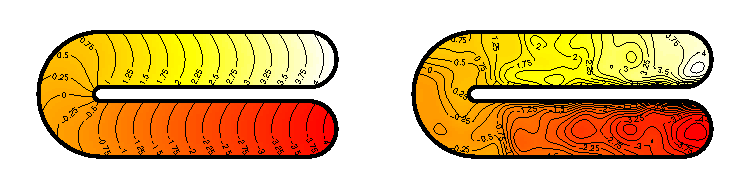
\includegraphics{intro/figs/ramsay-leak.pdf}\\
\caption{An example of leakage. A thin plate regression spline was fit to data sampled from the function on the left, here the model smooths across the gap in the middle of the domain (right.)}
\label{leakage}
\end{figure}

The problem of leakage arises because of the way in which the smoother defines how near objects are to one another. Most smoothing techniques use the Euclidean metric to measure the distance between data. Clearly though, this approach is a flawed: biological populations do not conform to Euclidean geometry in their movement patterns and hence their observed positions will reflect this. Just as whales no not uniformly distribute themselves across sea and glacier, fish do not lay their eggs on land. Natural and man-made barriers carve up the landscape (and seascape), partitioning biological populations; our models should take this into account.

The distribution of the population may be smooth, just not necessarily over $\mathbb{R}^2$ (\cite{wangranalli}). Instead the structure of the domain that is under investigation must be modelled (implicitly or explicitly) for the correct inference to be drawn.

\subsection{Ramsay's horseshoe function as a benchmark for finite area smoothing}

\label{ramsayfunc}

\cite{ramsay} proposes a function which can be used to benchmark new approaches to 2-dimensional smoothing. The function takes the form of a horseshoe shape which is flat across the domain has a gradient along the domain's major axis. This can be seen in \fig{orig-fs}. \cite{soap} modifies the test function by adding curvature across the minor axis of the shape. This was added in order to avoid the horseshoe function lying in the nullspace of their model's penalty, making the problem trivial. It is the second shape that will be used for simulations here and shall be referred to as the \emph{Ramsay horseshoe} throughout; it is shown in \fig{leakage}.

% original horseshoe from Ramsay's paper
\begin{figure}
\centering
% trim order l b r t
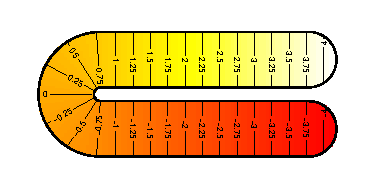
\includegraphics{intro/figs/orig-fs.pdf}\\
\caption{The horseshoe function as it appeared in \cite{ramsay}.}
\label{orig-fs}
\end{figure}

The test function highlights leakage well. As mentioned above, when the smoothing problem is specified in Euclidean distance, the model takes the distance between the points in the two arms of the horseshoe as the distance over the gap in-between them, rather than the distance along the major axis of the shape. This causes the high function values from one side to contaminate the other side (and the low to contaminate the high.) It is easy to see that this causes the smooth to be an inappropriate model.
		
\subsection{Previous approaches to leakage}

The cause of leakage can be characterised in two ways: either the smooth does not respect the boundary of the domain, or the smooth does not take into account the geometry of the domain (in particular with regard to the distance between points within the domain). Previous work in this area has been to combat leakage along these two lines. Work of \cite{ramsay} and \cite{soap} both use a partial differential equation (PDE) boundary condition approach to try to prevent leakage, where as \cite{wangranalli} and \cite{eilerstalk}  attempt to approximate the intrinsic structure of the domain while not treating the boundary as something special in the basis setup. These four main works may be summarised as follows:

\begin{enumerate}
\item \cite{ramsay} proposes finite element $L$-splines (FELSPLINEs). The $L$-spline replaces the usual penalty term (see \secref{GAMpenalties}) with:
\be
\int_\Omega (L_p f)^2 \text{d}\Omega,
\ee
where $\Omega$ is the domain in question and $L_p$ is a roughness operator defined as:
\be
L_p=\Delta^p+c_{p-1}\Delta^{p-1}+\dots+c_1\Delta+c_0I.
\ee
Here $I$ is the identity operator, the $\{c_0,\dots, c_p\}$ are constants and the $\Delta$ is the Laplacian ($\Delta f = f_{xx}+f_{yy}$ in the usual notation). Although any differential operator could, in principle, be used for $L_p$, the Laplacian gives rise to a set of polynomials which are rotation and translation invariant which is clearly sensible given the objective function solution should not depend on the coordinate system used.

In order to find the minimiser of the objective function, Ramsay takes a finite element approach. First he triangulates the domain, then he constructs a set of bivariate quadratic polynomial basis functions over each triangle, specifying that there be continuity over the edges of the triangles. By taking the FELSPLINE objective function and transforming it into a variational form (in the same way as a PDE is), the approximation to the minimiser of the objective function is found. 

Since the triangulation and hence the penalty of the FELSPLINE is only calculated over the domain, and the continuity is specified over neighbouring cells, the method prevents leakage. However, although FELSPLINE does not exhibit leakage on the original horseshoe (as in \fig{orig-fs}), in practice the model makes unrealistic physical assumptions. The boundary conditions of FELSPLINE specify that the gradient is zero, along normals to the boundary. This is not always physically realistic. \cite{soap} show that by using a different response function for the horseshoe shape, the FELSPLINE performance begins to falter.

FELSPLINE does not offer a realistic physical model and is therefore not a viable solution to the finite area smoothing problem in general.

\item \cite{wangranalli} adopt a ``within-area distance'' formulation for thin plate splines. They take the geodesic distance between two points, that being the shortest path within the domain. This gives a definition of how near objects are in the domain. 

Wang and Ranalli first create a weighted, undirected graph ($G$, say) with a data point at each vertex and the distance between each pair of vertices as the weights on the edges. They then take the restricted graph of $G$, $G_k$, in which each vertex is only connected to its $k$ nearest neighbours. With this new, restricted graph the geodesic distances between each pair of vertices can be calculated using Floyd's algorithm (\cite{Floyd}).

As the authors point out, the quality of the approximation is dependent on the size of the data set and its density. At low densities the estimated geodesic distance will tend towards the Euclidean, at high densities the approximation tends, asymptotically toward the true geodesic distance (\cite{bernstein}). Even if  dense enough data were available, the method will be rather slow since Floyd's algorithm is cubic in the number of vertices (the size of the data set). Finally, although the $k$-nearest neighbours algorithm used is not specified in the paper, in general such procedures are computationally expensive, adding another source of impedance to the technique.

Taking these points into account, Wang and Ranalli's approach appears cumbersome, slow and dependent on dense data.

\item The soap film smoother (\cite{soap}) uses a rather simple physical model to prevent leakage from occurring. First, consider the domain boundary to be made of wire, then dip this wire into a bucket of soapy water, you will then have (provided it doesn't pop(!)) a soap film in the same of your boundary. Now consider the wire to lie in the $x-y$ plane and the height of the soap film at a given point to be the functional value of the model. This film is then distorted smoothly by moving it toward the data, while minimising the surface tension in the film. The domain ($\Omega$) is bounded by some polygon with boundary conditions that are either known or estimated by a cyclic spline.

Mathematically, the soap film smoother is constructed by first specifying a set of functions $\rho_k(x,y)$, which are each solutions to the Laplace equation in two dimensions:
\be
\frac{\partial^2\rho}{\partial x^2} + \frac{\partial^2\rho}{\partial y^2} = 0
\ee
except at one of the knots ($x^*_k,y^*_k$). Then, solving Poisson's equation in 2-dimensions:
\be
\frac{\partial^2 g_k}{\partial x^2} + \frac{\partial^2 g_k}{\partial y^2} = \rho
\label{soap-poisson}
\ee
with $\rho=\rho_k(x,y)$, where $k$ indexes the knots and the boundary condition $\rho=0$. The set of basis functions for the soap film smoother, $g_k(x,y)$ is found, along with $a(x,y)$ (the solutions to \eqn{soap-poisson} when $\rho=0$, subject to the boundary condition). These bases are then summed to form:
\be
f(x,y)=a(x,y)+\sum_{k=1}^n \gamma_k g_k(x,y),
\ee
the soap film smoother, where the $\gamma_k$ are parameters to be estimated. The (isotropic) penalty term (\secref{GAMpenalties}) is:
\be
\int_\Omega \Big(\frac{\partial^2 f}{\partial x^2}+\frac{\partial^2 f}{\partial y^2} \Big)^2\text{d}x\text{d}y,
\ee
Differing from the standard \tprs penalty since: (\emph{i}) the integration occurs only over $\Omega$, (\emph{ii}) there is no mixed derivative term, and (\emph{iii}) the whole integrand is squared rather than each term individually. This allows the $x$ and $y$ term's derivatives to be traded off against each other so the nullspace of the penalty is infinite dimensional. This allows those functions in the nullspace to be sufficiently wiggly to meet any boundary conditions.

The solution of the PDEs above, yielding the basis and penalty, is the most computationally expensive part of the procedure. Knots to use for $x_k^*$ and $y_k^*$ must be specified, usually using a grid. Numerical problems occur when knots are placed in boundary cells in the PDE solution grid.

Although mathematically elegant, the soap film smoother is a rather complex model. It also treats the boundary differently from the interior and uses a cyclic spline in order to approximate the boundary values. This treatment of the boundary seems rather unnatural and it may not always be physically realistic to consider the boundary in such a way.

\item An alternative approach to treating the boundary as something special is to transform the space in which the points lie to instead lie in a different domain which is more suitable for smoothing. For example, with Ramsay's horseshoe, it seems intuitive to simply bend the horseshoe into a long strip and then smooth on that domain.

Indeed, \cite{eilerstalk} proposed using the \sch transform for this very purpose (I, independently, came to the idea in 2008 via BBC Radio 4.) Using the \sch transform for smoothing will be elaborated on in chapter \ref{chap-sc}, so only a brief summary is given here.

The basic idea is to find a function, $\phi$ say, that takes points in the domain the data lie in ($W$) and maps them to a domain ($W^*$) in which the boundary is less complex ($\phi : W \mapsto W^*$, mathematically).

Creating some kind of mapping between the space in which the data lies and the space in which conventional smoothers perform well is convenient. Not having to setup a new basis structure and relying on long tested methodology is clearly appealing. This approach also benefits from not treating the boundary as a special in the basis setup.
\end{enumerate}

Chapters \ref{chap-sc} and \ref{chap-mds} expand on the ideas in the last method; of using a transformation of space and conventional smoothers to solve the problem of leakage in finite area smoothing.

\section{Distance sampling}

This will be a very brief introduction to distance sampling methods, in the style of the encyclopaedia of environmetrics article.


\chapter{Modelling the spatiotemporal distribution of the incidence of resident foreign population in Italy}

\label{chap-it}

\citeb{Augustin2009} demonstrated the utility of a tensor product of a thin plate regression spline (for space) and a cubic spline (for time) in spatiotemporal smoothing. Using the soap film smoother described in chapter \ref{chap-intro} (in place of the thin plate spline), a spatiotemporal smooth is used to model the distribution of the incidence of the resident foreign population in Italy. This chapter presents the first application of this approach to spatiotemporal smoothing in a complicated geographic region. 

The work presented here is adapted from the article ``Modelling the spatiotemporal distribution of the incidence of resident foreign population in Italy'' by G. Marra (Statistical Science, University College London), D. L. Miller and L. Zanin (Prometia, Bolognia), accepted for publication in \textit{Statistica Neerlandica}. Each of the authors contributed equally to the article.

\section{Introduction \label{IN}}

\subsection{Background}

Many European countries have recently experienced a substantial increase in the proportion of immigrants in the population (\cite{Manning2010}). In particular this has increased since the introduction of new EU members in 2004 and 2007 (\cite{euexpansion}). 

Immigration statistics calculated at a national level do not provide information on the local spatial and temporal distribution of the phenomenon. This information may be of crucial importance for planning local policies. Using Italian data (at a municipal level) for the period 2003-2008, a tensor product smoother combining a cubic regression spline basis for time and a soap film spline basis for space can be used to create spatiotemporal maps. These maps could then be effectively used by policy makers to decide the allocation of economic resources at both a local and national level.

A \textit{municipality} (in Italian \textit{comune}) is the lowest level administrative sub-division in Italy. Municipalities then make up provinces (of which there are 110) which in turn make up regions (of which there are 20).

\subsection{Data}  

The \textit{resident foreign population} includes all people (born in Italy or abroad) who declare their citizenship not to be Italian. The change in resident foreign population at a municipal level, at the end of a year, is determined by
\begin{equation}
RFP^{31^\text{st}} = RFP^{1^\text{st}} + (I_1 + I_2 + I_3+ I_4) - (D_1 + D_2 + D_3 + D_4 + AC),
\label{it-rfp}
\end{equation}
where $RFP^{31^\text{st}}$ indicates the total number of resident foreigners at the end of December and $RFP^{1^\text{st}}$ the number of resident foreigners on the $1^\text{st}$ of January. $I_{1}$ denotes the number of people whose parents are foreigners (at least one of them being resident in the municipality), $I_{2}$ the number of foreign citizens who asked to transfer their residence from another Italian municipality to the current one, $I_{3}$ those who asked to transfer their residence from abroad, and $I_{4}$ refers to recording operations due to other reasons (e.g. foreigners mistakenly deleted from the registry of the municipality, because they were temporarily missing). $D_{1}$ represents the number of resident foreigners who died during the year, $D_{2}$ those who moved to a different municipality, $D_{3}$ those who moved abroad, $D_{4}$ refers to cancellations for other reasons (e.g. foreigners deleted from the registry of the municipality, because they were not present), and \textit{AC} denotes those resident foreigners who obtained Italian citizenship during the year. 

Given a specific area such as municipality (although this is often calculated on provincial, regional or national level too), a measure of density of resident foreign population is the percentage \textit{incidence of resident foreigners} (IRF), given as the ratio of the number of resident foreigners (the RFP) to the total resident population multiplied by 100 (e.g. \cite{Lowell2007}). This gives a simple demographic indicator for comparing different areas of a country in terms of number of resident foreigners per 100 resident inhabitants. According to ISTAT (the Italian government's statistical office), the IRF as calculated on a national level has grown substantially, from 2.7\% in 2002 to 6.5\% in 2008. 

Recently ISTAT has integrated the official statistics with a new public database (available via \url{http://demo.istat.it}), mainly based on administrative sources. The database gives the number of resident foreigners (calculated as above) in each of almost 8100 municipalities. Note that this does not include foreigners entering the country illegally, this issue is not addressed here. The quantification of illegal immigrants is an open topic of discussion in the studies of international migrations (e.g. \cite{Strozza2004}). Several approaches have been proposed in literature to quantify this, but all are subject to criticism (especially with regard to the magnitude of errors in estimates). Here only official data on the resident foreign population is considered. The ISTAT data, at a municipal level, (the highest resolution available at this time) is an excellent resource for creating maps.

\begin{figure}[tbp]
	\centering
		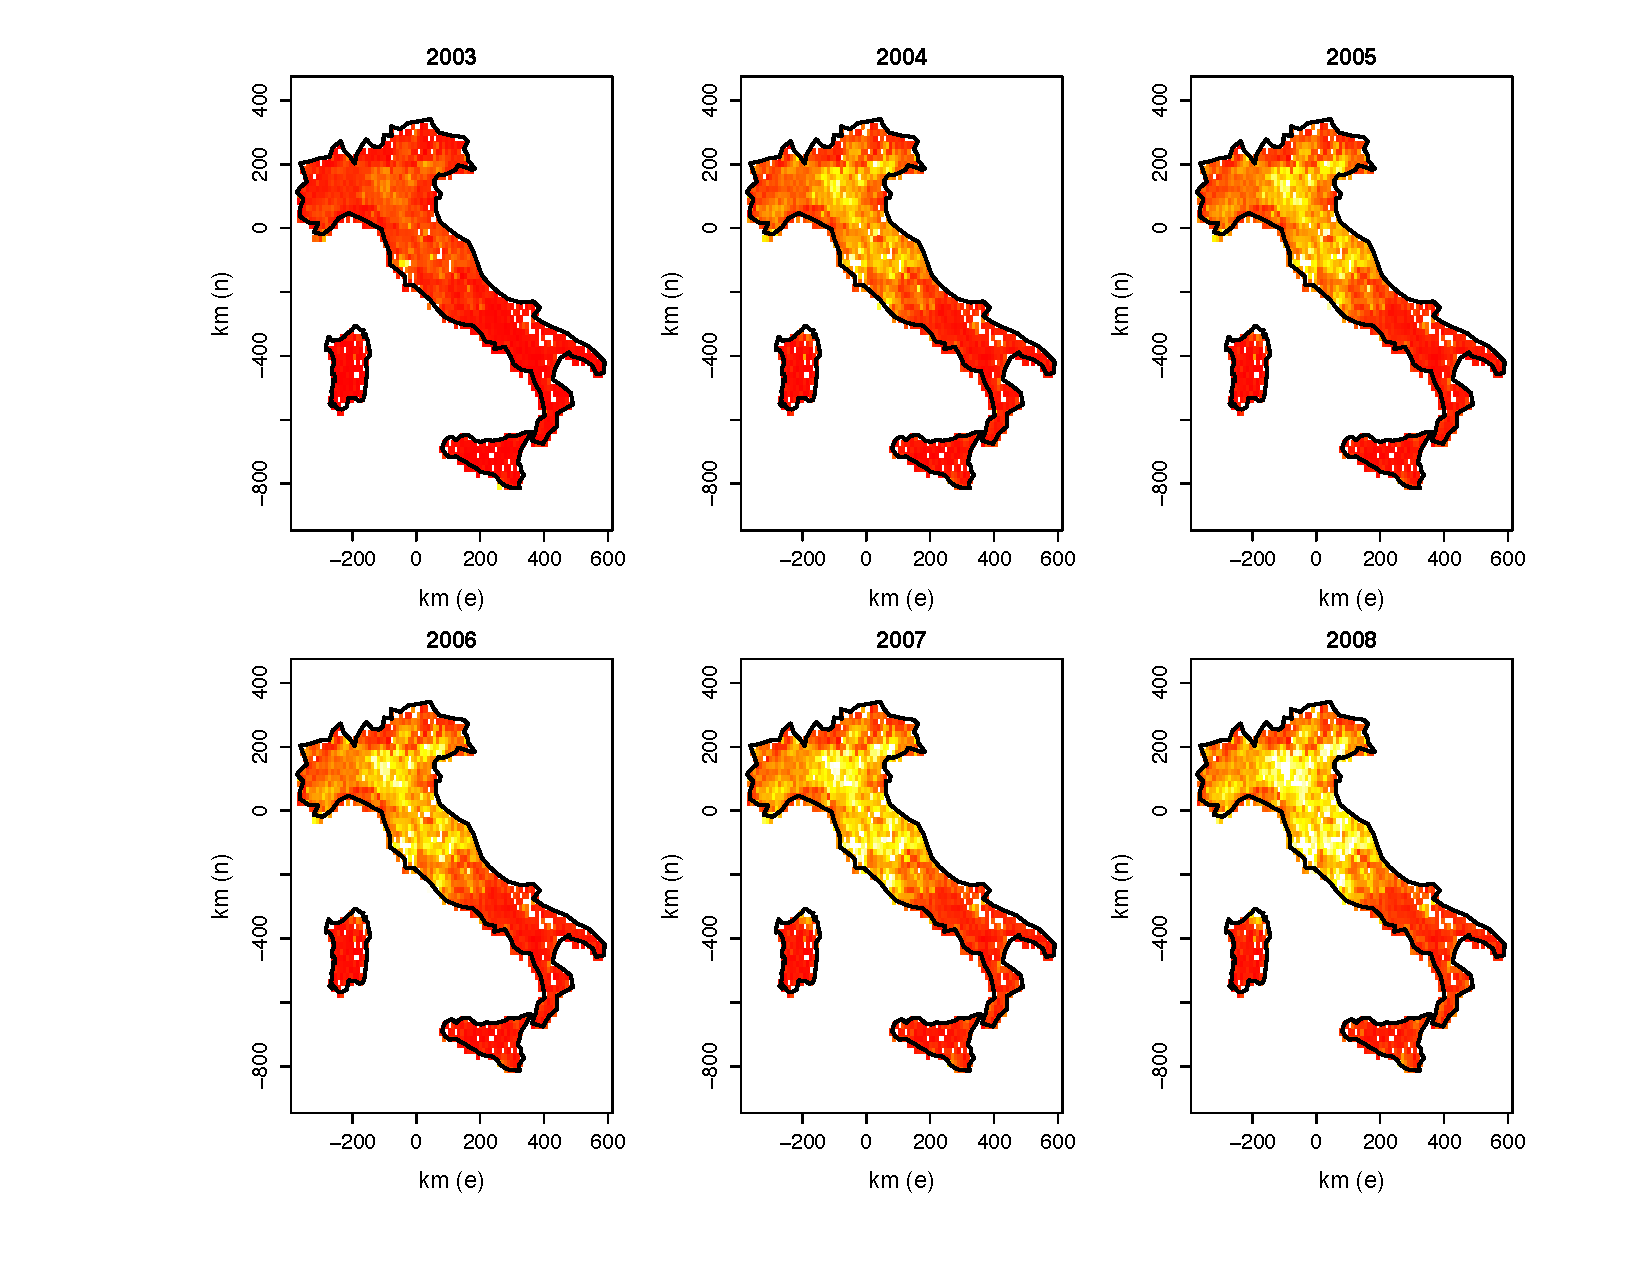
\includegraphics[width=\textwidth]{it/Raw}
	\caption{Empirical maps of the percentage incidence of resident foreigners in Italy over the years 2003-2008. These were obtained using ISTAT data at a municipal level.	The incidence is given as the ratio of the number of resident foreigners to the total resident population multiplied by 100. The colour scale ranges from an incidence of 0 (dark red) to an incidence of 12 (white).}
	\label{Rd}
\end{figure}

Figure \ref{Rd} shows plots of the raw IRF data at a municipal level over the years 2003-2008 (these are, of course, averaged over a grid for plotting purposes). The features that stand out clearly are the marked difference between north and south, and the increase in the IRF over time. However, these maps make it difficult to detect any local spatial structure in the incidence. For example, the Po Valley (northern Italy) has relatively high levels of IRF in 2008 but it is not really possible to clearly identify any particular areas of polarization. This can be problematic for policy makers in the central public administration who wish to allocate economic resources as efficiently and effectively as possible. Previous studies analysing the distribution of resident foreign population have employed descriptive analysis and/or to what amounts  to complex linear modelling approaches (e.g. \cite{Fonseca2008}, \cite{Longhi2010}). Using the soap silm smoother, high resolution spatiotemporal maps of the IRF can be created.


\section{The model \label{METH}}

There are currently no relevant economic covariates available at a municipal level, the response (IRF) is modelled using a smoother which is a function of only the spatial coordinates and time. The model is then used to create smoothed maps of the geographical area of interest over time. Two points are noteworthy here. First, since the coastline of Italy has a complex boundary, leakage (as described in \secref{intro-FAS}) is likely to occur; inappropriately linking parts of the domain could have serious policy implications. Second, looking at figure \ref{Rd}, there appears to be a strong temporal interaction (those places with high incidence increase their incidence over time) so the model used should account for a space-time interaction. These two goals can be achieved by using a generalized additive model incorporating a three-dimensional tensor product smoother combining a cubic regression spline basis (\secref{intro-cubic}) for the temporal trend and a soap film smoother (\cite{soap} and \secref{intro-FAS}) for the spatial component.

\subsection{Model specification \label{MS}}

As explained in the introductory section, the IRF is given as the ratio of the number of resident foreigners to the total resident population multiplied by 100. The IRF may therefore only take positive values. Letting $f$ be a smooth function, the proposed model is as follows
\begin{equation}
\log \left\{\mathbb{E}(\texttt{irf}_{it})\right\} = f(\texttt{year}_t,\texttt{n}_i,\texttt{e}_i), \ \texttt{irf}_{it} \sim \text{Tweedie}\left\{\mathbb{E}(\texttt{irf}_{it}),\phi \mathbb{E}(\texttt{irf}_{it})^{p}\right\},          
\label{PropM}
\end{equation}
at municipality $i=1,\ldots,8094$ and year $t=2003,\ldots,2008$. $\phi$ is a dispersion parameter and the log link function ensures positive fitted values. $\texttt{irf}_{it}$, $\texttt{n}_i$, and $\texttt{e}_i$ represent the variables percentage IRF, Northing and Easting, respectively. Tweedie distributions are a special case of an exponential dispersion model and include, for example, the normal ($p=0$), Poisson ($p=1$) and gamma ($p=2$) distributions (\cite{Jorgensen}). For $1<p<2$ Tweedie distributions can be represented as Poisson mixtures of gamma distributions, with mass at zero but otherwise continuous on the positive reals. These are especially appealing for modelling continuous positive observations when exact zeros occur. \citeb{Dunn2005} provides a survey of published applications stressing the utility and flexibility of this class of distributions. $f$ is a multidimensional smooth function of \texttt{year}, \texttt{n} and \texttt{e} which models the joint effect of these variables on \texttt{irf}. Northing and Easting are as described in \secref{intro-basic-setup} (in this case the offsets used were 11.5 longitude, 44 latitude), thus ensuring that the spatial part of the smoother is isotropic (which would not be the case if latitude and longitude were used).

\begin{figure}[tb]
	\centering
		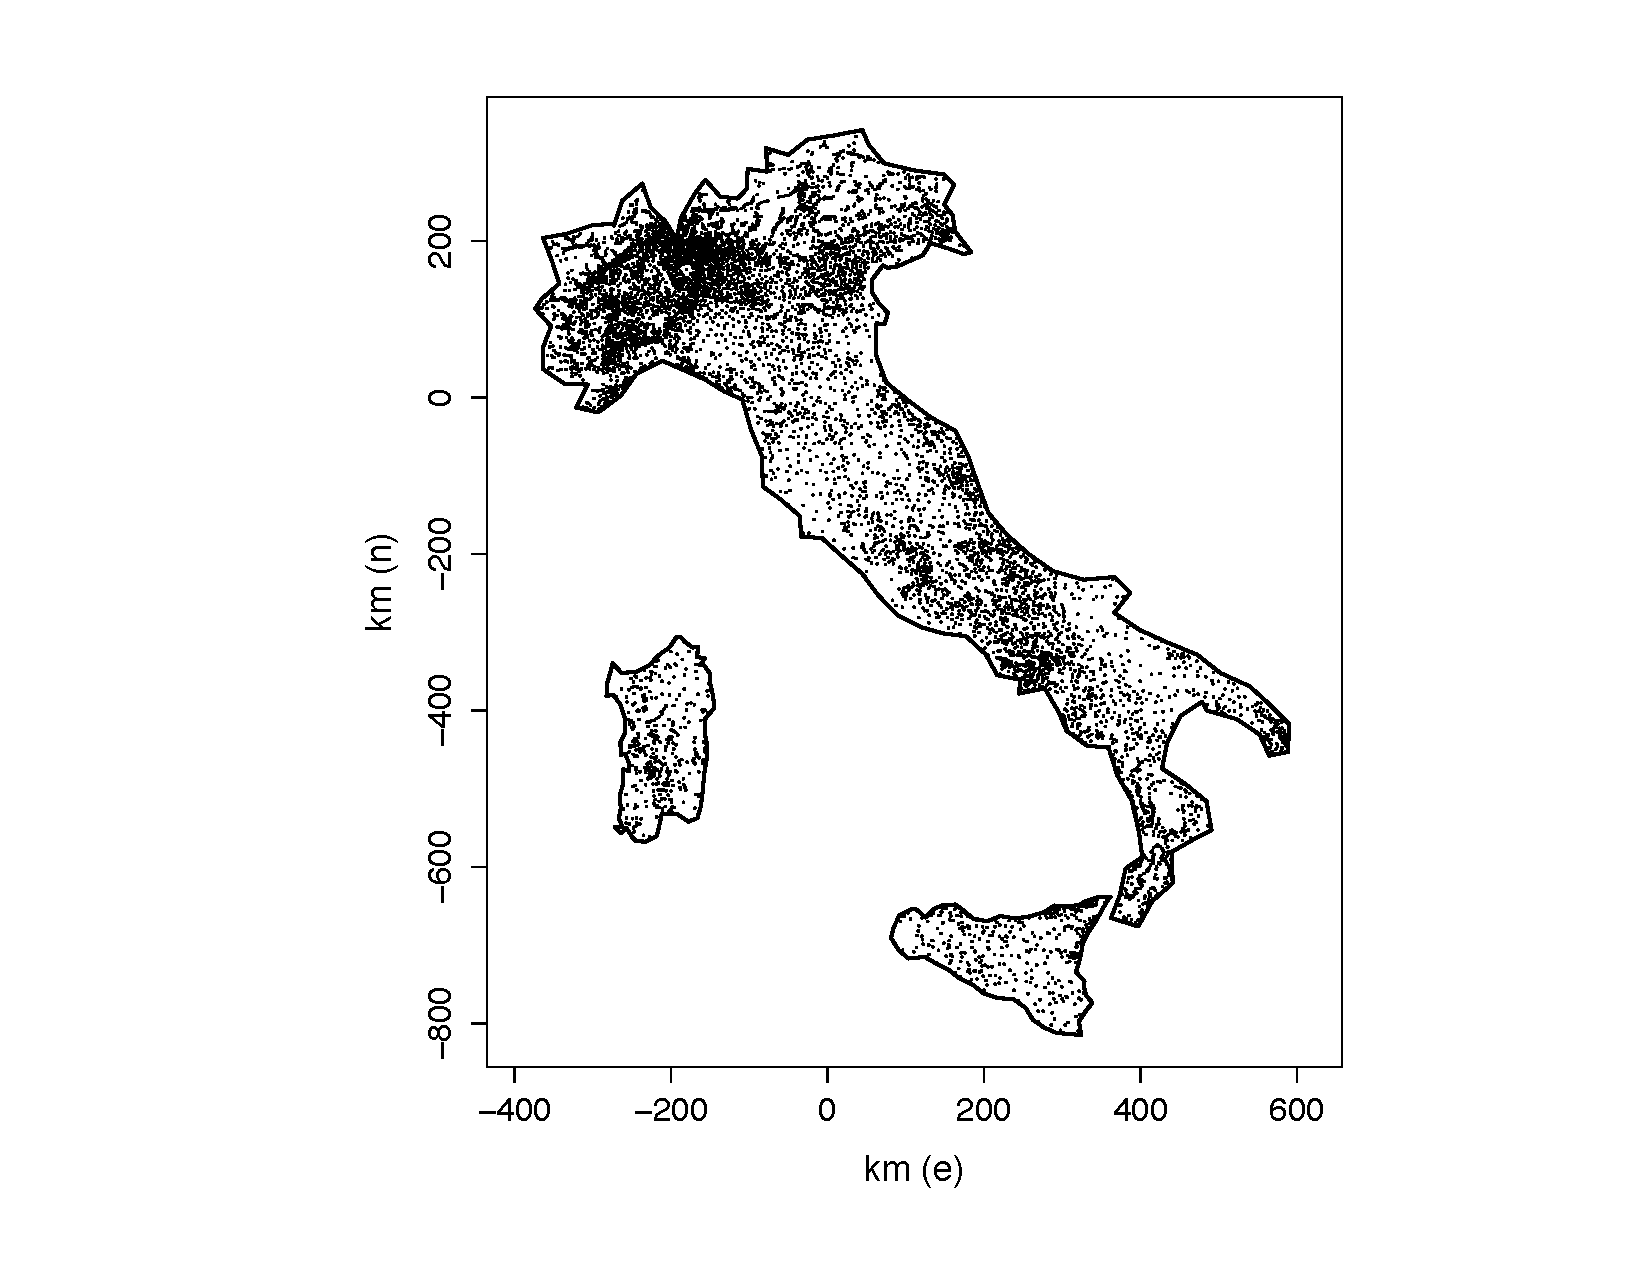
\includegraphics[width=3.5in]{it/pointmap.pdf}
	\caption{Raw data locations for the incidence of resident foreigners with the boundaries of Italy, Sardinia and Sicily. Each point is the location of the centroid of a municipality.}
	\label{pointmap}
\end{figure}

Note that the data were collected per municipality but enter into the model as points which are located at the centroids of the municipalities (see figure \ref{pointmap}). This change of support from areal to point data is not problematic and is desirable. The aim is to produce smoothed maps; using areal data would yield maps that are step functions for each municipality hence making it more difficult to see patterns in the data. To make the maps as easily interpretable as possible, smoothing of points is a clear choice.

The technical details of the construction of the smoothers is now covered. First, building on the general formulation given in \secref{GAMtensor}, the construction of a three-dimensional tensor product smoother is shown, using a one-dimensional temporal smoother and a two-dimensional spatial smoother. The details of the construction of the two-dimensional smoother, using the soap film smoother are then given. The final section details the construction of temporal trend estimates.

\subsection{A three-dimensional tensor product smoother for time and space \label{3D}}

The tensor product smooth used here is similar to the one shown in \secref{GAMtensor}, however it differs in two ways.  First, one of the components is a two-dimensional, isotopic spatial smooth ($f_\text{year}$) and the other component ($f_\text{space}$) is a marginal one-dimensional smooth of time. Second, the size of each basis is different.

Omitting the subscripts $i$ and $t$ for simplicity, the temporal smooth $f_\text{year}$ and spatial smooth $f_\text{space}$ can be written in terms of their basis decompositions (as in (\ref{intro-basisdecomp})):
\begin{equation*}
%f_\text{year}(\texttt{year})=\sum_{l=1}^L \xi_l b_l(\texttt{year})=\textbf{X}_\text{year}\bm\xi \ \ \text{and} \ \ f_\text{space}(\texttt{n},\texttt{e})=\sum_{r=1}^R \varphi_r d_r(\texttt{n},\texttt{e})=\textbf{X}_\text{space}\bm\varphi,
f_\text{year}(\texttt{year})=\sum_{j=1}^J \xi_j b_j(\texttt{year}) \ \ \text{and} \ \ f_\text{space}(\texttt{n},\texttt{e})=\sum_{r=1}^R \varphi_r d_r(\texttt{n},\texttt{e}),
\end{equation*}
where the $b_j(\texttt{year})$ and $d_r(\texttt{n},\texttt{e})$ are known cubic regression spline and soap film basis functions (respectively), with corresponding parameters $\xi_j$ and $\varphi_r$ and spline dimensions $J$ and $R$. 

In order to set up a three-dimensional tensor product smoother for time and space it is necessary for $f_\text{year}(\texttt{year})$ to vary smoothly with the spatial dimensions. This can be achieved by allowing the parameters $\xi_j$ to vary smoothly with \texttt{n} and \texttt{e}. Using the spline set-up for $f_\text{space}(\texttt{n},\texttt{e})$ we may write (analogously to \secref{GAMtensor}):
$$
\xi_j(\texttt{n},\texttt{e})=\sum_{r=1}^R \varphi_{jr} d_r(\texttt{n},\texttt{e}),
$$    
which results in:
$$
f(\texttt{year},\texttt{n},\texttt{e})=\sum_{j=1}^J \sum_{r=1}^R \varphi_{jr} d_r(\texttt{n},\texttt{e}) b_j(\texttt{year}). 
$$

To calculate the penalty, first let $J_\text{year}$ and $J_\text{space}$ be measures of the wigglyness of the functions $f_\text{year}$ and $f_\text{space}$ respectively. For $f_\text{year}$, the second-order cubic spline penalty evaluates $J_\text{year}(f_\text{year})=\int\left( \partial^2 f_\text{year}/\partial \texttt{year}^2 \right)^2 \text{d}\texttt{year}$ (\secref{intro-cubic}). The penalty for the soap film smoother used for the spatial part of the tensor product is covered in the next section; for ease of explanation it is treated as a black box here.

An overall penalty for the tensor product smoother can be obtained by applying the penalties of $f_\text{space}(\texttt{n},\texttt{e})$ to the varying coefficients of the marginal smooth $f_\text{year}(\texttt{year})$, $\xi_l(\texttt{n},\texttt{e})$,
$$
\sum_{j=1}^J J_\text{space}\left\{  \xi_l(\texttt{n},\texttt{e}) \right\},
$$ 
and the penalties of $f_\text{year}(\texttt{year})$ to the varying coefficients of the marginal smooth $f_\text{space}(\texttt{n},\texttt{e})$, $\varphi_r(\texttt{year})$,  
$$
\sum_{r=1}^R J_\text{year}\left\{  \varphi_r(\texttt{year}) \right\}.
$$ 
It follows that the penalty of $f(\texttt{year},\texttt{n},\texttt{e})$ can be written:
\begin{equation}
\lambda_\text{space} \sum_{j=1}^J J_\text{space}\left\{  \xi_l(\texttt{n},\texttt{e}) \right\} + \lambda_\text{year} \sum_{r=1}^R J_\text{year}\left\{  \varphi_r(\texttt{year}) \right\},
\label{it-fullpen}
\end{equation}
where as usual, $\lambda_\text{space}$ and $\lambda_\text{year}$ are the smoothing parameters for time and space respectively.

\Secref{intro-cubic} gives the details of the cubic spline basis used to model the temporal part of the smooth. The next section shows how $f_\text{space}$ and $J_\text{space}$ are constructed.

\subsection{The soap film smoother \label{SF}}

Since there is no particular reason to believe that the resident foreign population should be continuous across physical boundaries such as the Mediterranean Sea (at best there are merely potential resident foreigners in the sea), a smoother which takes into account of the fact that the borders of Italy represent both physical barriers should be used. Although there is no reason \textit{a priori} to believe that there will be particularly troublesome leakage (see \secref{intro-FAS}) here, mitigating against the issue by use of appropriate basis function choice from the outset is the most sensible course of action. 

As mentioned in \secref{intro-leakageapproaches}, the soap film smoother (\cite{soap}) uses a rather simple physical model to prevent leakage from occurring. First, consider the domain boundary to be made of wire, then dip this wire into a bucket of soapy water; a soap film with the same shape as the boundary will have then formed. Now consider the wire to lie in the $\texttt{n}$-$\texttt{e}$ plane and the height of the soap film at a given point to be the functional value of the model. This film is then distorted smoothly by moving it vertically toward each datum locally, while minimizing the surface tension in the film as a whole. Mathematically, the domain ($\Gamma$) is bounded by some polygon ($B$). For the islands of Sicily and Sardinia is their coastlines and for for the mainland is its coastline along with the border with France, Switzerland, Austria and Slovenia to the north. Note that a separate model was used for each of the mainland and Sardinia and Sicily (see \secref{ER} for why this was necessary).

The soap film smoother basis is quite similar in form to the thin plate regression spline basis given in \secref{GAMtprs}. The basis is split into two sets of functions to form a smoother that respect the necessary boundary conditions. The first basis is used for the smoothing within the region of interest, $\Gamma$; the second is to deal with the boundary, $B$. These two sets of basis functions are then summed to form:
\begin{equation*}
f_\text{space}(\texttt{n},\texttt{e})=\sum_{j=1}^J \alpha_j a_j(\texttt{n},\texttt{e}) + \sum_{k=1}^K \gamma_k g_k(\texttt{n},\texttt{e}),
\end{equation*}
where the $\gamma_k$ and $\alpha_j$ are the parameters to be estimated. One can think of the $a_j(\texttt{n},\texttt{e})$ as an offset dictated by the estimated boundary conditions on $B$ (similar to the linearly independent polynomials in the thin plate spline, although it is important to note that these functions are not planes) and the sum of the $g_k(\texttt{n},\texttt{e})$ as the smooth function to the data inside $\Gamma$ (analogous to the radial basis functions in the thin plate spline). Unlike thin plate splines however, the soap film basis requires the specification of $K$ knots inside $\Gamma$ and $J$ boundary knots on $B$ (here a grid is used for the internal knots and the boundary knots are equally spaced along $B$, further detail on the setup used is given in \secref{ER} and table \ref{soap-basis-table}). For convenience later, the second sum is labeled as $f_\text{int}$ (the part of $f$ with knots inside $\Gamma$). The rest of this section shows how these bases are constructed.

For the internal part of the smoother we first find a set of functions $\rho_k(\texttt{n},\texttt{e})$. These are each solutions to the Laplace's equation in two dimensions
$$
\frac{\partial^2\rho}{\partial \texttt{n}^2} + \frac{\partial^2\rho}{\partial \texttt{e}^2} = 0,
$$
except at one of the knots ($\texttt{n}^*_k,\texttt{e}^*_k$). Then, solving Poisson's equation in 2-dimensions
\begin{equation}
\frac{\partial^2 g_k}{\partial \texttt{n}^2} + \frac{\partial^2 g_k}{\partial \texttt{e}^2} = \rho_k(\texttt{n},\texttt{e}),
\label{soap-poisson}
\end{equation}
for $k$ indexing the $K$ knots. When the boundary condition $\rho_k(\texttt{n},\texttt{e})=0$ is applied, the set of basis functions for the soap film smoother $g_k(\texttt{n},\texttt{e})$ are found.  The partial differential equations (PDEs) are solved numerically using a multi-grid solver (e.g. \cite[pp. 862-880]{press1992numerical}), see the appendix of \cite{soap} for further technical details.

To find the height of the function at each point around the boundary a cyclic spline basis is used to construct $f_\text{bnd}(r)$. This $f_\text{bnd}(r)$ will have the expansion
\begin{equation}
f_\text{bnd}(r)=\sum_{j=1}^J \alpha_j \delta_j(r),
\label{soap-cyclic}
\end{equation}
where $r$ is the distance along the boundary, the $\alpha_j$ are parameters and $\delta_j(r)$ are cubic spline basis functions. The basis functions have the same form as the cubic spline discussed in \secref{intro-cubic}, but to ensure that the spline is cyclic the value of the function at the first knot is constrained to be the same as that at the last knot up to their second derivatives. Note that  the values of the $\alpha_j$ are not of interest at this stage, only the basis expansion. The basis functions $a_j(\texttt{n},\texttt{e})$ can be found by solving (\ref{soap-poisson}) for $\rho_k(\texttt{n},\texttt{e})= 0$ with the boundary condition resulting from setting $\alpha_j=1$ (and all other $\alpha_i$ to zero) in (\ref{soap-cyclic}), using the same methods as for the $g_k(\texttt{n},\texttt{e})$ above. Each $a_j(\texttt{n},\texttt{e})$ can then be thought of as the function with a peak at the corresponding knot on $B$, which are smooth across the whole of $\Gamma$.

The set of basis functions of $f_\text{int}$ have been found, as well as the boundary-induced-smooth which acts as a base for the soap film smoother. Although this seems like a rather esoteric setup, all the procedure above is effectively doing is setting up a basis such that standard penalized regression techniques can be used. Just as one might choose one spline basis over another for some property it possesses, the soap film basis has the property that it obeys the (estimated) boundary conditions of the region that are to be smoothed over.

In \secref{3D} the spatial penalty term was simply referred to as a single quantity, however (as was the case with the basis) the penalty is split into two parts: one for the cyclic smoother around the boundary and the other for the internal smoother. The easiest way to think about this is to write the spatial part of the penalty given in (\ref{it-fullpen}) as:
\begin{equation*}
\lambda_\text{space} \sum_{j=1}^J J_\text{space}\left\{  \xi_l(\texttt{n},\texttt{e}) \right\} = \lambda_\text{int} J_\text{int} + \lambda_\text{bnd} J_\text{bnd}.
\end{equation*}
The smoothing parameter $\lambda_\text{space}$ is not estimated and only exists as a way of making the tensor product explanation above clearer. The two interior and boundary penalties are now considered individually.

%Writing $\bm\beta$ as the vector of all smooth coefficients for the soap film, $\bm\gamma$ for the boundary parameters and $\bm\alpha$ for the interior, we have
%$$
%\bm\beta^\text{T}\textbf{S}^*_\text{space}\bm{\beta} = \lambda_\text{bnd} \bm\gamma^\text{T}\textbf{S}_\text{bnd}\bm{\gamma} + \lambda_\text{int} \bm{\alpha}^\text{T}\textbf{S}_\text{int}\bm{\alpha},
%$$
%where 
%$$
%\textbf{S}^*_\text{space} = \lambda_\text{bnd} \textbf{S}_\text{bnd} + \lambda_\text{int} \textbf{S}_\text{int}.
%$$
%$\textbf{S}^*_\text{space}$ is the total penalty for the spatial part of the smoother, $\textbf{S}_\text{int}$ is the interior penalty and $\textbf{S}_\text{bnd}$ is the cyclic spline boundary penalty. Both are matrices of known coefficients depending on the chosen basis functions. The $\lambda$ are the smoothing parameters for the boundary and interior smooth terms respectively. As in the previous section, for mathematical convenience, an asterisk indicates that the penalty matrices have been multiplied by the appropriate smoothing parameters. We now look at the two parts of the penalty individually. 

The isotropic interior penalty term is calculated as
$$
J_\text{int} = \int_\Gamma \Big(\frac{\partial^2 f_\text{int}}{\partial \texttt{n}^2}+\frac{\partial^2 f_\text{int}}{\partial \texttt{e}^2} 
\Big)^2\text{d}\texttt{n}\text{d}\texttt{e}.
$$
Note that the integration occurs only over $\Gamma$ rather than over the whole of $\mathbb{R}^2$ as would usually be the case. Also, there is no mixed derivative term, and the whole integrand is squared rather than each term individually (in contrast with, say, a thin plate regression spline penalty given in (\ref{tprs-pen})). This allows the $\texttt{n}$ and $\texttt{e}$ terms' derivatives to be traded off against each other so that the nullspace of the penalty is infinite dimensional. This permits those functions in the nullspace to be sufficiently wiggly to meet any boundary conditions. Note the similarity to the FELSPLINE penalty in \secref{intro-leakageapproaches}.

The penalty for the cyclic spline running about the boundary, used to estimate the $\alpha_j$, is calculated as 
$$
J_\text{bnd} = \int_B \Big(\frac{\partial^2 f_\text{bnd}}{\partial r^2}\Big)^2 \text{d}r.
$$
where the basis functions are the cubic regression splines defined above, but with the additional condition that the function's values and their first and second derivatives at the first and last knot must be equal. See e.g. \cite[p. 149]{simonbook} for more details.

The smooth function for $f_\texttt{space}$ obtained using the construction outlined above is rotationally invariant. Two smoothing parameters are estimated for the soap film (one for the interior and one for the boundary) but each controls the smoothness for both geographical directions at once (\cite{soap}). However, the tensor product smoother using the cubic regression spline basis for time and a soap film for space is not isotropic in space-time. This anisotropy is desirable since, as explained in Section \ref{MS}, the measurements of space and time are on different scales so it would not make sense to estimate one smoothing parameter for both the spatial and temporal components (e.g. \cite[p. 162]{simonbook}).
 
 In all, two smoothing parameters are estimated for the soap film ($\lambda_\text{int}$ and $\lambda_\text{bnd}$), and one for the temporal component ($\lambda_\texttt{year}$). Models were run using both REML and GCV for smoothness selection (with no major differences between the two methods). The results presented here are those for REML as described in \secref{intro-otherGAMfit}.
 
To summarize, the basis functions $a_j(\texttt{n}_i,\texttt{e}_i)$ and $g_j(\texttt{n}_i,\texttt{e}_i)$, and the penalties $J_\text{bnd}$ and $J_\text{int}$ have been found. Soap basis functions and penalties can be obtained using the the \textsf{R} package \texttt{soap} which implements the ideas discussed in this section.

\subsection{Variance and trend estimation \label{VE}}

Taking a Bayesian view it is possible to construct intervals using the posterior distribution of the model parameters. The interesting feature of these intervals is that, since they include both a bias and a variance component, they have good observed \textit{frequentist} coverage probabilities across the function (\cite{Marra2011}). The posterior distribution is given as
\begin{equation}
\bm\beta|\texttt{irf} \dot{\backsim} N( \hat{\bm\beta}, {\bf V}_{\bm\beta} ),
\label{Poster}
\end{equation}
where $\hat{\bm\beta}$ is the maximum penalized likelihood estimate of (all of) the smoother's parameters, $\bm\beta$ (i.e. concatenating all of the parameters discussed above into one vector). ${\bf V}_{\bm\beta}$ is of the form $(\mathbf{X}^\text{T}{\bf W}\mathbf{X}+{\bf S}^*)^{-1}\phi$, $\mathbf{X}$ contains the columns associated with the regression spline bases used to set up the model, ${\bf W}$ and $\mathbf{z}$ are the weight matrix and the pseudodata vector at convergence of the algorithm used to fit the penalized model and $\phi$ is the scale parameter (as in \secref{intro-extending-gams}). Given result (\ref{Poster}), confidence intervals for linear functions of the parameters can be found easily. Intervals for non-linear functions of the model coefficients can be conveniently obtained by simulation from the posterior distribution of $\bm\beta$. To aid interpretation of the results, trend estimates for some given areas of interest can be produced using the predictive distribution of $\texttt{irf}_{it}$, using the method proposed in \citeb{Augustin2009}. This approach can be implemented as follows:

\begin{enumerate}
	\item Repeat the following steps for $b=1,\ldots,N_b$, where $N_b$ represents the number of random draws. 
	   \begin{enumerate}
	      \item Simulate a random $N(\hat{\bm\beta}, \hat{{\bf V}}_{\bm\beta} )$ and call the resulting coefficient vector $\bm\beta_b$.
	      \item Calculate $\widehat{\mathbb{E}(\texttt{irf}_{it})}=\widehat{\texttt{irf}}_{itb}=\exp(\mathbf{X}^*_{it}\bm\beta_b)$, where $\mathbf{X}^*_{it}$ is evaluated at the observed values. 
	      \item For a given area of interest $a$ and year $t$, calculate
	      $$\widehat{\overline{\texttt{irf}}}_{tb}^a=\frac{1}{n_a}\sum_{i=1}^{n_a} \widehat{\texttt{irf}}_{itb},$$
	      where $n_a$ represents the number of observations in area $a$.     
	   \end{enumerate}
	\item Produce the required summary statistics, in this case median, lower and upper $95\%$ quantiles, for the temporal trend $\widehat{\overline{\texttt{irf}}}_{tb}^a$.
\end{enumerate}
Small values for $N_b$ are typically tolerable. In practise, $N_b$ can be set to $100$. Increasing this value does not change the results which are presented in the next section.
 

\section{Results \label{ER}}

The model was implemented using the basis sizes (for the cubic and cyclic regression splines) and interior knots (for the soap film) given in table \ref{soap-basis-table}. Note that separate models were used for each of mainland, Sicily and Sardinia since scenarios with multiple islands are not currently supported in the \texttt{soap} package.

\begin{table}[t]
\centering
\begin{tabular}{c c c c}\\
Region & Interior knots & Cyclic spline basis size & Cubic spline basis size\\
\hline
Mainland & 41 ($14 \times 14$) & 20 & 6\\
Sardinia & 12 ($5 \times 6$) & 8 & 6\\
Sicily & 12 ($6 \times 6$) & 10 & 6\\
\end{tabular}
\caption{Basis sizes per region for the smooth functions to be fitted to the Italian data. For the interior (soap film) knots, the numbers in brackets show the initial grid, the other number gives the number of knots actually used (those inside the boundary).}
\label{soap-basis-table}
\end{table}

The parameter for the Tweedie distribution ($p$ in (\ref{PropM})) was set to $1.2$. It was chosen by trial and error to produce the best possible residual plots. The estimate for $\phi$ was equal to $0.905$. Before employing the class of Tweedie models, simpler gamma distribution-based models were used; diagnostic plots suggested the presence of substantial structure in the residuals. Residual analysis was carried out following an approach similar to that of Chandler (2005). Figure \ref{Resid} gives some diagnostics for the proposed model. Overall, the first two sets of boxplots do not show long-term trends, but suggest the presence of some spatial residual structure. The normal Q-Q plot shows some curvature in the upper tail. The scale-location plot indicates the presence of some heteroskedasticity, although the LOESS smooth running though the plot (grey line) does not indicate a relationship between absolute residuals and predicted values. The presence of extreme values in all diagnostic plots suggest under-estimation of the IRF on occasion. Descriptive analysis revealed that some municipalities have considerably higher IRF levels compared to those in neighbouring municipalities. This is mainly due to the specific socio-economic features of attractiveness of each municipality which need to be accounted for in order to avoid under-estimation. Unfortunately, as pointed out in the introduction, currently no relevant economic data are available at a municipal level and hence such information can not be incorporated in the model. The deviance explained was 57\%. 

As a check, the proposed model was fitted again but replacing the response variable with the residuals. The resulting maps suggested the presence of some residual structure in those municipalities characterized by very high IRF levels; this was expected given the presence of extreme residuals evidenced in the diagnostic plots. Sensitivity analysis showed that the results do not change if more basis functions are used for the smooth term in the model. 

\begin{figure}[tbp]
	\centering
		\includegraphics[width=0.75\textwidth, angle=270]{it/Resid.eps}
	\caption{Deviance residual diagnostics from the spatiotemporal model of the incidence of resident foreigners. Row-wise from top: (i) yearly distributions, (ii) distributions of residuals grouped according to squares on a 10x10 grid which fell inside the boundary, (iii) normal Q-Q plot, (iv) absolute residuals versus predicted values, with LOESS curve (grey line).}
	\label{Resid}
\end{figure}

The proposed model was compared with one in which the spatial and temporal effects were simply additive. As in \citeb{Augustin2009}, Schwarz's Bayesian Information Criterion (BIC, see e.g. \cite[p. 286]{burnhamanderson}) was used to compare the two models; the latter yielded an increased BIC. Visually comparing the maps produced by these two models, the proposed model contained details that could not be seen in the model where the spatial and temporal effects were additive.

Despite the lack of fit corresponding to those municipalities characterized by very high levels of the IRF, the analysis above suggests that the proposed model is able to capture the overall spatiotemporal structure present in the data. Should some relevant economic variables become available at a municipal level, the model specification and, as a consequence, its explanatory power could be considerably improved. 

\subsection{Spatiotemporal maps \label{STT}}

As mentioned in the introductory section, Italy's national IRF was 6.5\% in 2008. Obviously, this number says nothing about specific local areas with particularly high or low levels of resident foreigners. Moving to smaller aggregations (say, the regional or provincial level) the same argument holds: some information is lost. This kind of low resolution statistic can mask smaller-scale heterogeneity in the population. Our aim here is to capture exactly this spatial heterogeneity.

At first glance, figure \ref{Rd} shows the stark contrast between north and south. The maps also highlight the inhomogeneous spatial and temporal distribution of the IRF. However, as pointed out above, smoothed maps can give a much better picture of the distribution of the IRF. Smoothing the maps allows for the separation of signal and noise in the data, giving a an idea of the overall structure of the phenomena, as well as providing a trend information via a temporal component of the model. Figure \ref{it-fig1} shows smoothed spatiotemporal maps of the IRF in Italy for the period 2003-2008, obtained using the approach described in the previous sections. The maps show that in 2003 northern and central Italy have the highest levels IRF. Over the subsequent years (2004-2008), the incidence spreads, forming four main areas where resident foreigners tend to live. Focusing on 2008, the most popular areas are in north Italy, specifically the Emilia-Romagna and Lombardy regions (with captials Bologna and Milan, respectively). These, although popular in 2003, appear to have increased their incidence. The second most attractive area is made up of the central Italian regions of Tuscany, Umbria, Marche and Lazio. The final two areas are composed of Liguria and Piedmont, and Veneto, Friuli-Venezia Giulia and Trentino-Alto Adige, in the northwest and northeast of the country, respectively. There is also an interesting growth in the incidence at the Swiss and Austrian borders (from about 2\% in 2003 to about 4-5\% in 2008). Resident foreigners seem less attracted by the regions and islands of southern Italy. Returning to the Po Valley area, the maps in figure \ref{it-fig1} allow us to identify the presence of two large, well defined polarization patterns in the IRF, the first in the centre of the Po Valley and the second near Venice. The maps in figure \ref{Rd} do not reveal these patterns.

\begin{figure}[t]
	\centering
		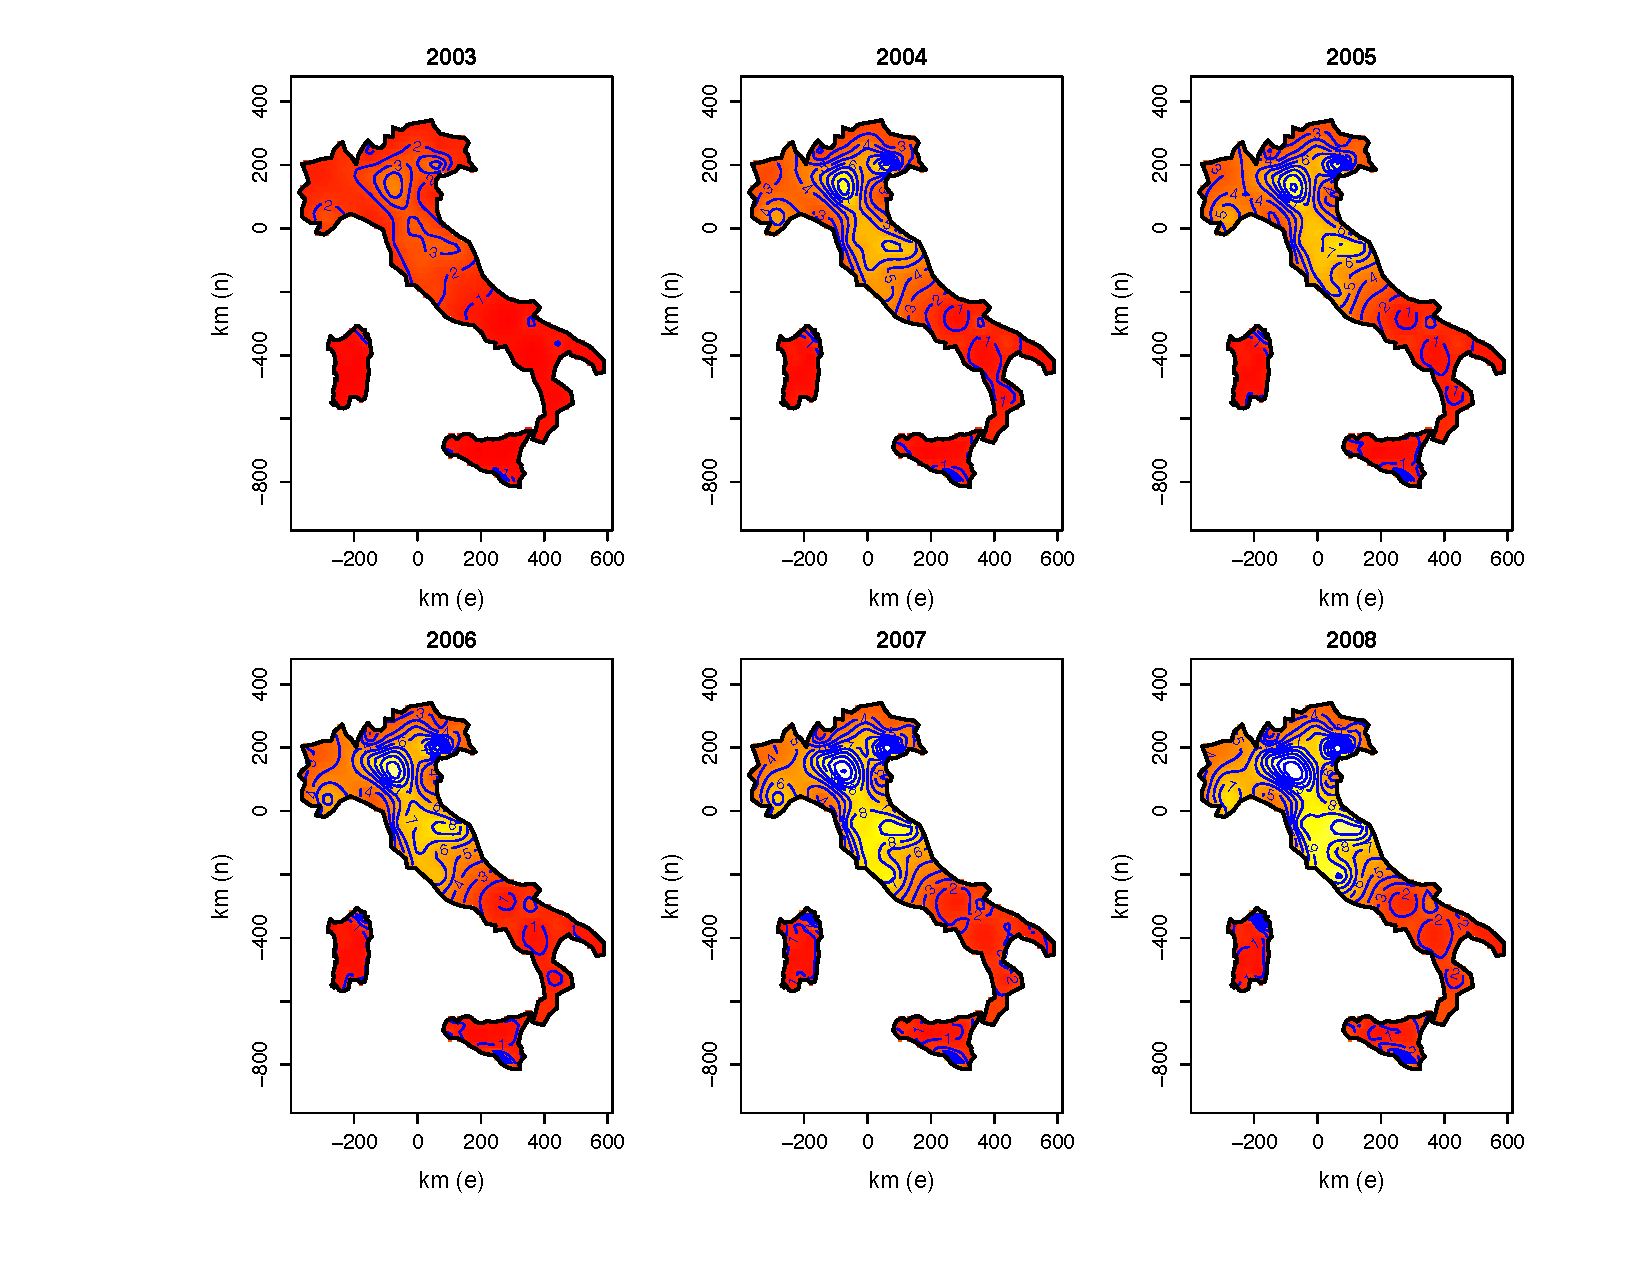
\includegraphics[width=\textwidth]{it/maps-Soap.pdf}
	\caption{Spatiotemporal maps of the percentage incidence of resident foreigners in Italy over the years 2003-2008. These were obtained using model (\ref{PropM}) with a tensor product smoother based on a cubic regression spline basis for time and a soap film spline basis for space, and ISTAT data at a municipal level. Predictions were made over those points lying inside the study region from a 100 by 100 grid. The incidence is given as the ratio of the number of resident foreigners to the total resident population multiplied by 100. The colour scale ranges from an incidence of 0 (dark red) to an incidence of 12 (white). Blue lines indicate contours separated by a one unit change in incidence.}
	\label{it-fig1}
\end{figure}

Figure \ref{trends} shows the estimated temporal trends for both the full Italian territory and broken down by area with 95\% confidence intervals (using the approach in \secref{VE}). The trends for northern and central Italy are similar. However, those for southern Italy and the islands are much flatter. Northern and central Italy also show a faster growth in incidence. Such differences are supported by the confidence intervals. Overall, these trends reflect what we see in the maps in figure \ref{it-fig1}, that there is a significant difference between northern/central Italy and the south of the country and its islands. Note that, since the approach outlined in \secref{VE} cannot account for the presence of residual correlation structure, one would expect the obtained confidence intervals not to be exactly representative than those that might be produced when adjusting for such correlation. The most obvious approach would be to fit a generalized additive mixed model (\cite[chapter 6]{simonbook}) with a carefully chosen correlation structure. Unfortunately convergence problems prevented such a model from being fitted.

\begin{figure}[t]
	\centering
		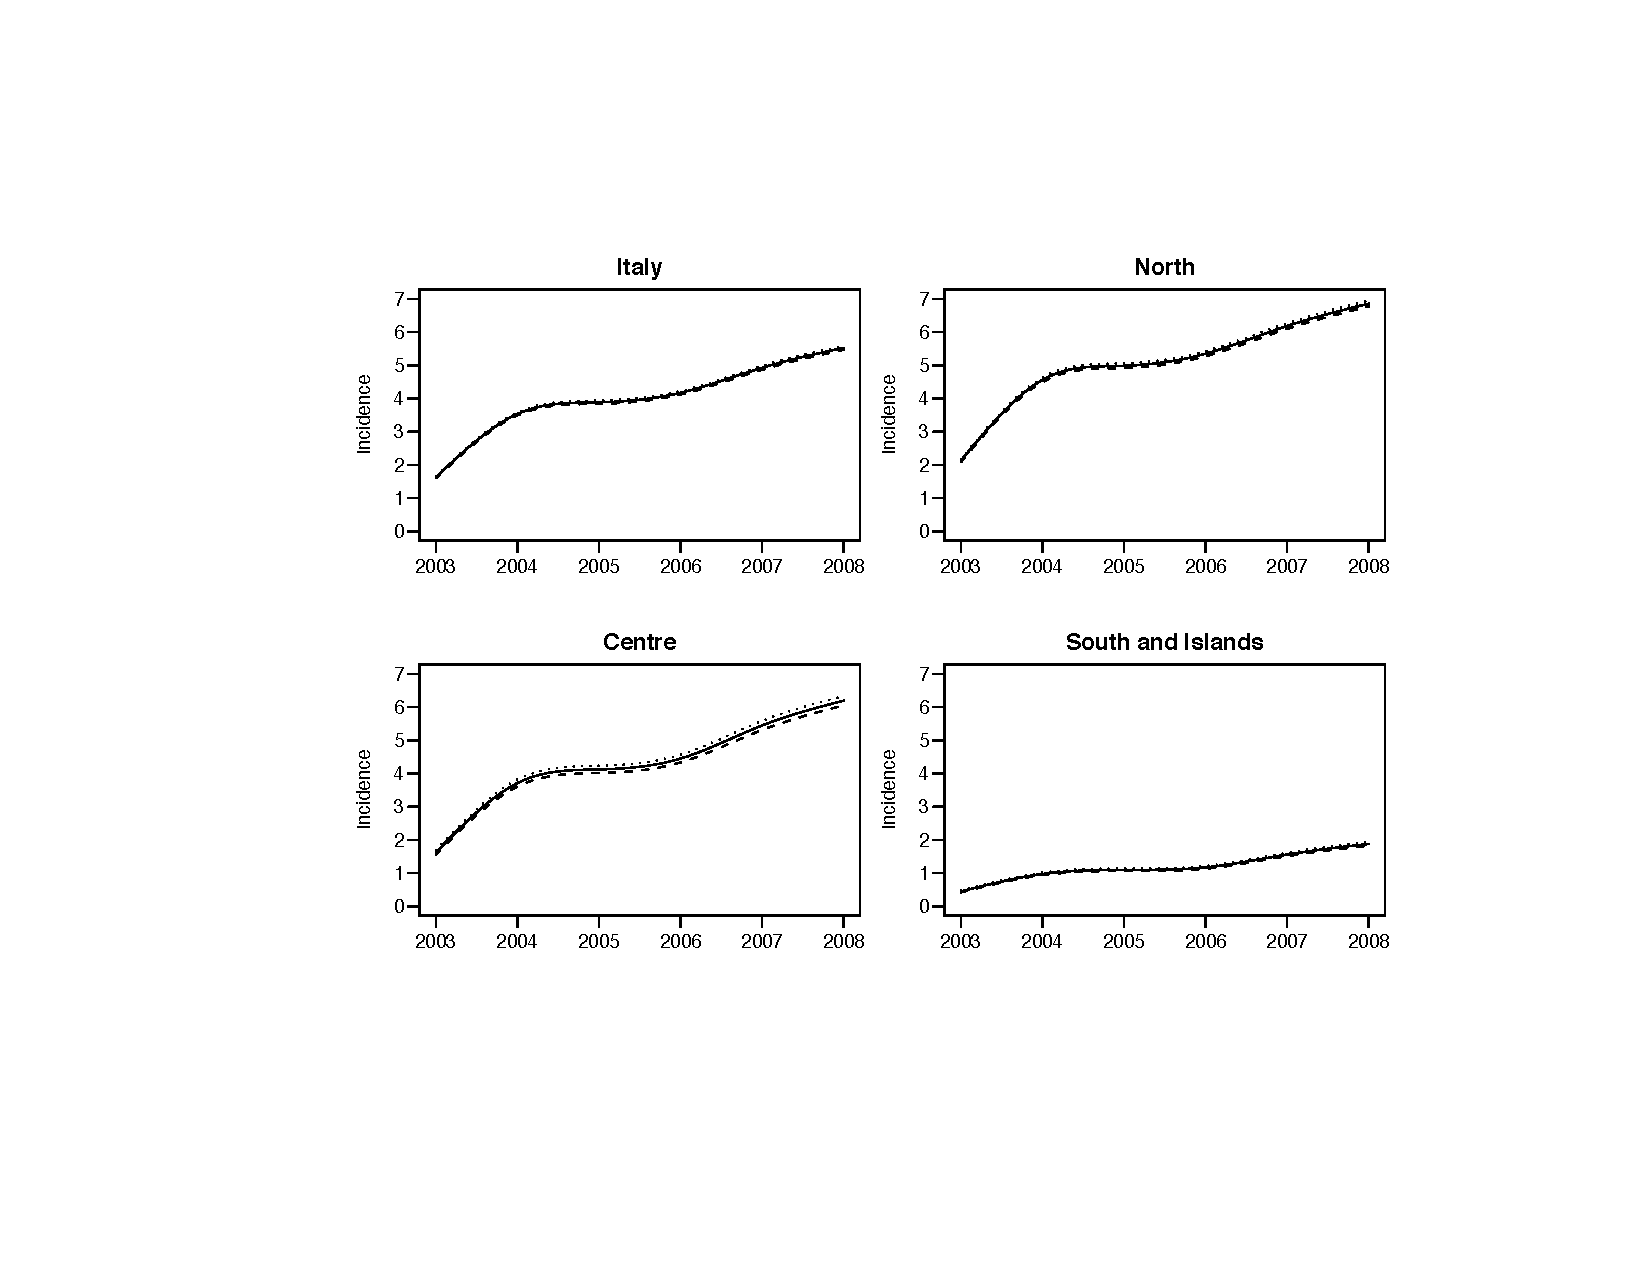
\includegraphics[width=\textwidth]{it/trends.pdf}
	\caption{Temporal trends in incidence of resident foreigners over the study period for Italy (top left), followed by trend estimates for north, central and south and islands areas with 95\% confidence intervals. North was defined as those points in the prediction grid above -20 km north, central as between -20 km and -300, and south and islands (including Sardinia and Sicily) as below -300.}
	\label{trends}
\end{figure}

The results presented in this section can be useful for policy-makers who may want to allocate economic resources as efficiently and effectively as possible, supporting, for instance, policies and services needed for the integration of resident foreigners. Such policies relate to a number of services such as: admission to education, access to the public health service, professional training, services supporting the match of labor supply and demand. For sociologists and demographers these maps may represent a new way to model spatiotemporal demographic changes and display the results graphically. 

\section{Conclusions}
\label{it-conc}

This chapter has shown an application of the soap film smoother as part of a larger spatiotemporal model. It has also hopefully shown that the models defined in chapter \ref{chap-intro} can be usefully applied to spatial smoothing as well as illustrating the modelling process.

The smoothed maps show in figure \ref{it-fig1} and the trends in figure \ref{trends} show that modelling the incidence of resident foreigners properly can give a much better picture of the distribution of the IRF as compared to just looking at the empirical maps in figure \ref{Rd}. The maps clearly show which parts of Italy are more popular with resident foreigners and the temporal trends gave an indication of the differences between different areas over time (in particular north and south). This information may be crucial for policy-makers who may want to allocate economic resources as efficiently and effectively as possible for supporting (for example) policies and services needed for the integration of resident foreigners.

Should some relevant economic variables become available at a municipal level, logical extensions incorporating covariate effects could be considered. This might assist in determining what further factors effect the distribution of resident foreigners in Italy and further aid decision making.

Using a tensor product of the soap film with the cubic regression splines allowed for the full interaction between the spatial and temporal components of the model. This approach is relatively simple to implement thanks to the ease of developing such models using the \textsf{R} packages \texttt{mgcv} and \texttt{soap}. There were, however, some difficulties. Specifically, it was not possible to build a model for both the mainland and islands simultaneously, which would allow for the estimation of a single temporal smooth for the whole of the country. It is also unfortunate that it was not possible to fit a generalized additive mixed model to take into account the correlation in the data, this was due to numerical issues (in particular the optimization procedure failed to converge).

This analysis has given some idea of the practical considerations from the point of view of an investigator when smoothing over regions with complex boundaries. Being able to code models in a familiar environment makes the process of developing a model much easier (writing the model definition in \textsf{R} for the model used here is only marginally more complicated than that for a more standard GAM). Keeping within the GAM framework allows for the usual diagnostic procedures to be used, making model checking straightforward. On an extremely practical level, it was apparent that the amount of time that it takes to fit the model becomes a serious consideration during development (not only due to the author's relative lack of patience); waiting for models to fit or to fail to converge can cause frustration and only acts as a barrier to wide-adoption. The methods developed in the coming chapters should take this into account.




\chapter{Using the \sch\ transform to morph domains for finite area smoothing}
%\begin{quotation}
%``Failure is \textit{always} an option.'' 
%
%-- Adam Savage
%\end{quotation}

% schwartz-christoffel stuff

\label{chap-sc}

\section{Introduction}

This chapter investigates the efficacy of using a conformal mapping to transform the domain in which we wish to perform smoothing. The mapping takes points in the domain of the data ($W$) to a domain on which it is easier to smooth ($W^*$). In particular the utility of the \sch transform is examined (elaborating on \cite{eilerstalk}).

Given some region that it is difficult to smooth over, one approach is to transform the domain in which the problem resides. So, for example, one could transform a region into a rectangle, circle or other familiar shape to avoid the problems such as leakage. In this spirit, we wish to find some mapping such as $\phi$ in \fig{simpledia}.

This kind of approach is appealing since it allows the use of existing techniques in the transformed domain (\emph{ie.} not having to resort to model and basis reformulation). It also feels more natural to treat the domain as if it were made of silly putty and simply squash the region into the shape required to perform analysis.

% Simple diagram showing the mapping
\begin{figure} [htbp]
\centering
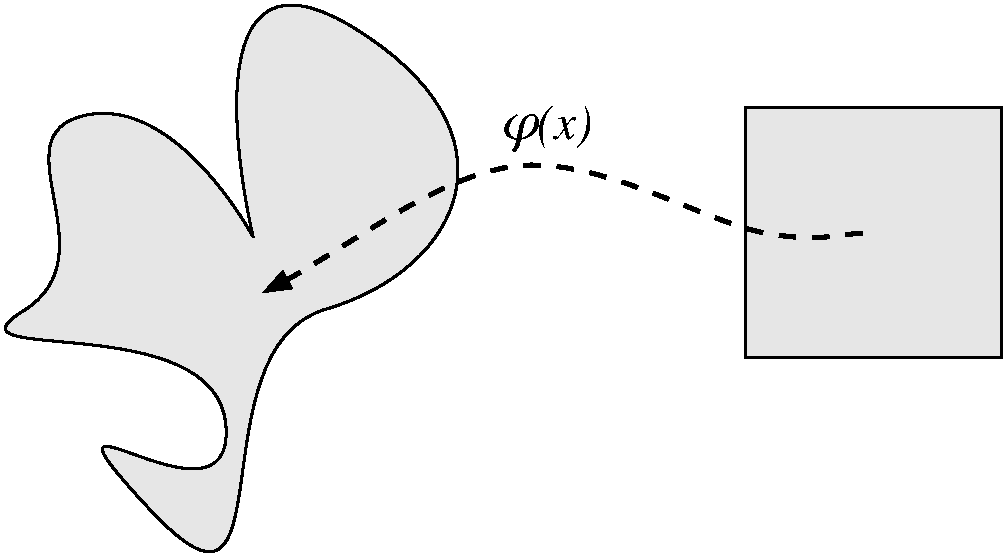
\includegraphics[scale=0.3]{sc/figs/simpledia.pdf}
\caption{An example of a transformation; the function $\phi$ takes the points in the rectangle and maps them to the region on the left.}
\label{simpledia}
\end{figure}

The \sch mapping offers such a transformation; it takes some arbitrary polygon and maps it to some specified shape. The most common domains to transform to are: (i) the upper half-plane ($H^+$), (ii) a rectangle and (iii) the unit disk. This is achieved in the $H^+$ case by taking the vertices of the polygon and mapping them to points on the real line (see \fig{reallinedia}). This can be thought of as ``unwrapping'' the polygon onto the real line. For the unit disk case, points on the circle bounding the unit disk map to vertices on the polygon (see \fig{unitdiskdia}). One can think of this as adding control points to the unit circle and then altering the angles. The rectangular case is somewhat similar to the unit disk in that extra points are added to the boundary and the angles of these points tightened until the shape is identical to the polygon. Obviously, those points lying inside the polygon are also moved around due to the mapping, creating a new (non-uniform) distribution of space.

% Diagram showing upper half plane to polygon
\begin{figure} [tbp]
\centering
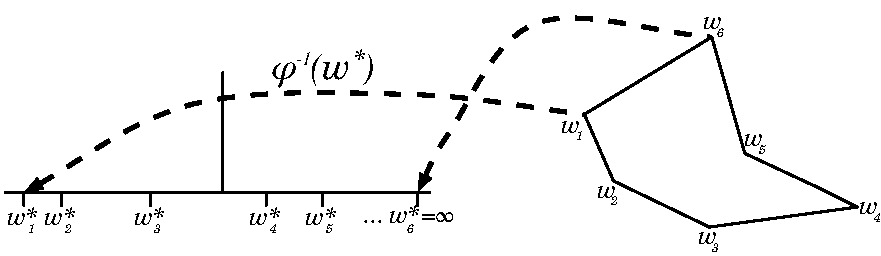
\includegraphics[scale=0.6]{sc/figs/reallinedia.pdf}
\caption{A mapping of the upper half-plane to the polygon. The vertices ($w_k$) are the result of applying $\phi$ to the points on the real line ($w^*_k$). The boundary of the polygon is mapped to the real line. Note that the final vertex, $w^*_6$ is mapped to the point $\infty$ on the real line.}
\label{reallinedia}
\end{figure}

% Diagram showing unit disk to polygon
\begin{figure} [tbp]
\centering
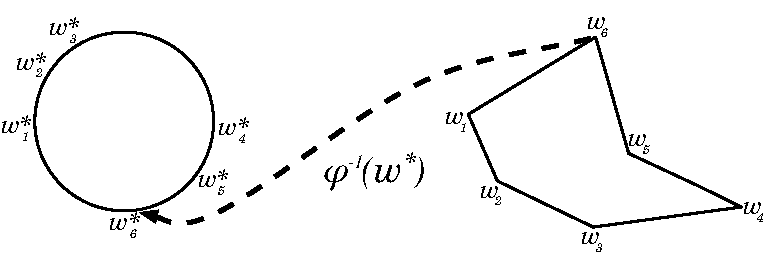
\includegraphics[scale=0.6]{sc/figs/unitdiskdia.pdf}
\caption{A mapping of the upper half-plane to the polygon. The vertices ($w_k$) are the result of applying $\phi$ to the points on the real line ($w^*_k$). The boundary of the polygon is mapped to the boundary of the unit disk.}
\label{unitdiskdia}
\end{figure}

The goal is to transform the domain with the complex boundary, then smooth in the transformed domain. The procedure we wish to perform is as follows:

\begin{enumerate}
\item Determine the domain over which we would like to smooth, $W$. This could be the region or a bounding box around it.

\item Compute the \sch transform of $W$ to get $W^*$. Obtaining the function, $\phi$.

\item Map the co-ordinates of the datapoints in $W$ to $W^*$.

\item Smooth the data in $W^*$.

\item Perform any further inference (in $W$ or $W^*$, since there is a 1-1 mapping between them).
\end{enumerate}

The second section of this chapter explains the technical details of the mapping. The third section gives results of some simulations and the final section summarises the results and draws conclusions from them.

\section{Technical details}

This section gives some of the mathematical and computational details required to calculate the \sch mapping. The primary reference is the extremely thorough work of \cite{driscoll}, which covers almost all aspects of the \sch transform.

\subsection{Nomenclature}

The polygon is first defined formally along with its associated quantities, as they will be referred to throughout the rest of the chapter.

A polygon, $\Gamma$, is a collection of vertices $w_1, w_2,\dots,w_n$ and interior angles $\alpha_1\pi, \alpha_2\pi, \dots, \alpha_n\pi$. For convenience we define $w_{n+1} = w_1$ and $w_0=w_n$. Numbering of vertices is anti-clockwise. The angles are such that $\alpha_k \in (0,2]$ and we require:
\begin{equation}
\sum_{k=1}^n (1-\alpha_k) = 2.
\end{equation}
The external angle, $\theta_k\pi$, as given by $(1-\alpha_k)\pi$ (see \fig{anglediagram}).

% Diagram showing the exterior/interior angle relationship.
\begin{figure} [bp]
\centering
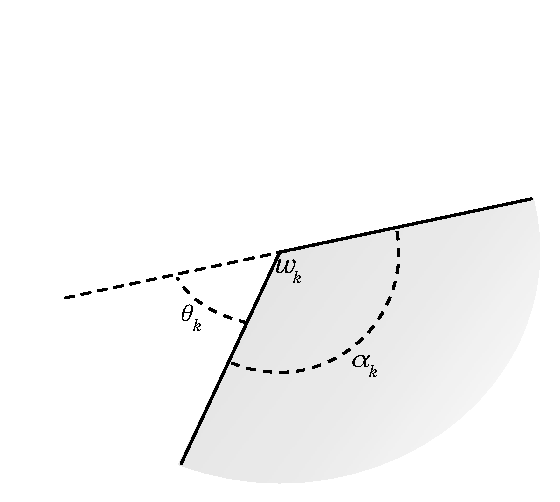
\includegraphics[scale=0.6]{sc/figs/anglediagram.pdf}
\caption{The external angle $\theta_k$ is associated with the vertex $w_k$. The internal angle is given by $\alpha_k$. Shading indicates the inside of the polygon.}
\label{anglediagram}
\end{figure}

The boundary of the polygon is denoted by $\Gamma$. We refer to two domains: $W$ and $W^*$, denoting the original domain (inside $\Gamma$) and the transformed domain (of the plane, unit disk or rectangle) respectively. 

Vertices on the polygon are denoted as $w_k$ and those on the transformed boundary are denoted as $w^*_k$ (the \emph{prevertices}). In general a point in the polygon's original domain is denoted as $w$ and in the transformed domain as $w^*$.

We use the function $\phi$ to map from the transformed domain to the polygon (\emph{ie.} $\phi:W^* \mapsto W$). The inverse mapping function, $\phi^{-1}$, is used to go from the polygon to one of: the unit disk, rectangle or half-plane ($\phi:W \mapsto W^*$).  See \fig{mappingdia}.

% Mapping diagram from my whiteboard
\begin{figure} [tbp]
\centering
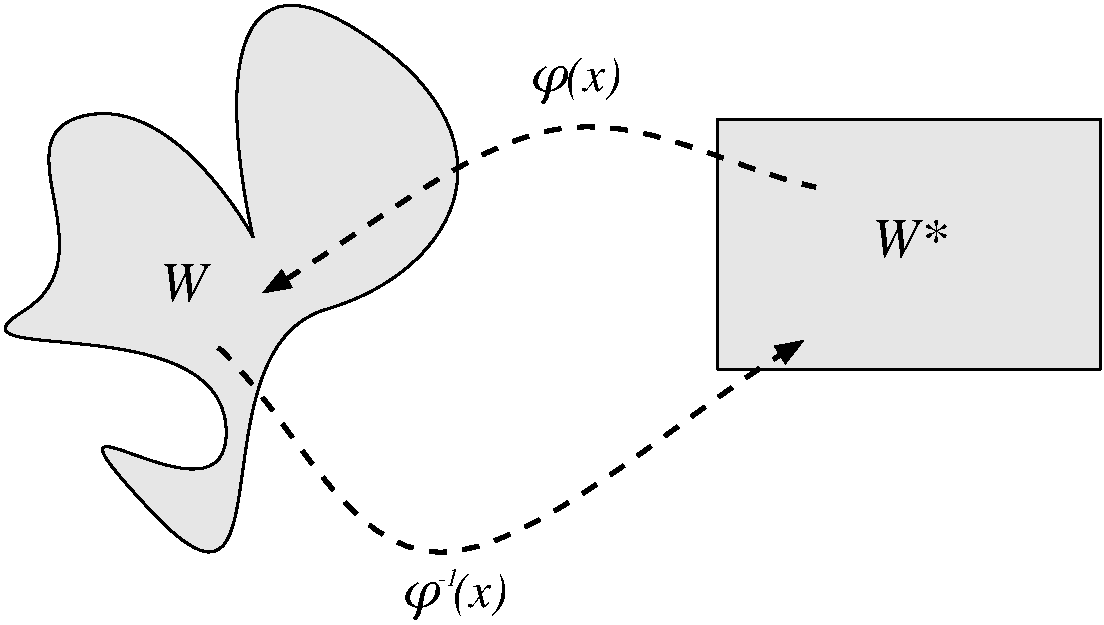
\includegraphics[scale=0.5]{sc/figs/mappingdia.pdf}
\caption{Diagram showing the forwards and backwards mappings with their relations to the mapped and unmapped spaces in the rectangular case.}
\label{mappingdia}
\end{figure}

\subsection{\sch Mapping}
\label{schparprob}
We now look at the mathematical formulation for the upper half-plane, unit disk and rectangle. There are many mappings that can be performed however those detailed here are either canonical (in the case of the half-plane) or considered to be useful in a smoothing context (the other two).

For the purposes of smoothing we are interested in the function $\phi^{-1}$ (\emph{ie.} the function that goes from our domain to the transformed one). We must first calculate $\phi$ before we may calculate its inverse. In the literature $\phi$ is referred to as the \emph{forwards map} and $\phi^{-1}$ as the \emph{backwards map}.

The forwards map, $\phi$, is determined up to translation, scaling, and rotation by the prevertices (see below). So, our task is to efficiently find the prevertices and hence find the mapping $\phi$. The task of obtaining the prevertices is known as the \emph{\sch parameter problem}.

\subsubsection{The upper half-plane}
\label{sc-parprob}

When mapping $\Gamma$ to $H^+$ we set $\phi(\infty) = w_n$ without any loss of generality. \cite{driscoll}, p. 10 then gives the following formula formula:
\begin{equation}
\phi(w^*) = A + C \int^{w^*}_{w^*_0} \prod_{k=1}^{n-1} (\zeta-w^*_k)^{\alpha_k-1} d\zeta.
\end{equation}
Here $A$ and $C$ are complex constants determined once the $w^*_k$ have been calculated. These control the scaling, translation, and rotation of the transform.

Although setting $\phi(\infty) = w_n$ does not make any difference in a mathematical sense, it does mean that the density of the points mapped into $H^+$ is rather odd. Given two adjacent points near $w_n$, their spacing on the upper half-plane is huge in comparison to two adjacent points near the other vertices. For this reason the $H^+$ mapping is not pursued further here.

\subsubsection{Unit disk}

The formula for the unit disk looks very similar to that for $H^+$ but the product now runs over all prevertices. The integrand is simply a constant multiple of the $H^+$ case. This is merely to avoid problems in the calculation of the branch cuts (\cite{driscoll}, p. 12).
\begin{equation}
\label{unitscmap}
\phi(w^*) = A + C \int^{w^*}_{w^*_0} \prod_{k=1}^{n} (1 - \frac{\zeta}{w^*_k})^{\alpha_k-1} d\zeta.
\end{equation}
As above, $A$ and $C$ are complex constants responsible for scaling, translation, and rotation.

\subsubsection{Rectangle}
For the rectangle case we must specify four vertices of $\Gamma$ that map to the four corners of the rectangle. This uniquely specifies the aspect ratio of the rectangle (\cite{driscoll}, p. 48).

The rectangle mapping is slightly different in its calculation to the two above mappings. We first map $\Gamma$ to the upper half-plane as detailed above. From there we can use the Jacobi elliptic function (\cite{handbuch} p. 701):
\be
F(\gamma,k)=\int_0^\gamma \frac{dt}{\sqrt{1-k^2\sin^2t}}
\ee
to map a rectangle to the upper half-plane. The computation of this map is expensive due to the evaluation of the elliptic function (\cite{driscoll}, \emph{p. 49}) so a shortcut is used by mapping to the strip. We do not go into further about detail here (as the computational intricacies are covered in \cite{howell90}).

\subsection{Computation of the \sch mapping}

To compute the map, we need to find the prevertices, $w^*_k$; since the complex constants just control scaling, translation, and rotation, we can compute them after computing the $w^*_k$. We achieve this iteratively by approximating the $w^*_k$ then mapping those points back to the polygon to give an estimate to $\Gamma$, $\Gamma^\prime$. 

To measure the quality of approximation of $\Gamma^\prime$ to $\Gamma$ we use the following set of equations:
\begin{equation}
\label{optimizeme}
\frac{\vert \phiinv(w_{k+1}) -  \phiinv(w_k) \vert}{\vert \phiinv(w_2)-\phiinv(w_1)\vert} - \frac{\vert w^*_{k+1} - w^*_k\vert}{\vert w^*_2 - w^*_1\vert} = 0, \qquad \text{for } k=3,\dots,n-1.
\end{equation}
Here $\vert \phiinv(w_{k+1}) -  \phiinv(w_k) \vert$ is the distance between the $k^{\text{th}}$ and $(k+1)^{\text{th}}$ vertex.  We find this by integrating along the line between the points within $W$.

Intuitively, we are comparing the side lengths of the polygon in order to evaluate approximation of $\Gamma$ in each iteration (\cite{snider}, A-3). Both of these measures are scaled by the distance between the first two vertices (in their respective domains).

Note that \eqn{optimizeme} does not include the vertex $w_n$. By theorem 3.1 of \cite{driscoll}, p. 24) a polygon is precisely defined by its angles and its vertices not including $w_n$ (since if we know the direction of the edges leaving $w_1$ and $w_{n-1}$, we may find the point where they meet). It is for this reason, in the upper half-plane case, that we can map $w_n$ to $\infty$ without loss of generality.

Also note that \eqn{optimizeme} does not include $w_1$ or $w_2$ in the numerator on the right hand side. This is due to all vertices (and hence $w_1$ and $w_2$) being rescaled, rotated, and translated by the complex constants, $A$ and $C$, in the \sch formula.

In practice we fix $w^*_n=1$, $w^*_{n-1}=-i$ and $w^*_{n-2}=-1$ in the unit disk case (\cite{driscoll}, p. 24). For the rectangle case we need to specify which vertices of $\Gamma$ will map to which vertices of the rectangle.

The scaling factor, $C$, (from \eqn{unitscmap}) may be calculated using:
\begin{equation}
C=\frac{\vert \phiinv(w_2)-\phiinv(w_1)\vert}{\vert w_2 - w_1\vert}.
\end{equation}
Otherwise, we can assume that up to scaling and rotation that $w_1$ and $w_2$ are correct. In which case we know that $\Gamma$ and $\Gamma^\prime$ are similar (in the geometric sense). 

$A$ is the image of the base point of the integration and is usually written as $w_0$. For computational reasons this is usually the prevertex nearest to the point $w^*$ that we wish to map in \eqn{unitscmap}  (\cite{driscoll}, \emph{p. 27}).


\subsubsection{Sketch of an algorithm to calculate the \sch mapping}
\label{algorithmsketch}
\begin{enumerate}
\item Accept inputs:
   \begin{enumerate} 
      \item $w_1,\dots,w_n$ (the vertices),
      \item $n$ (the number of vertices),
      \item $\alpha_1,\dots,\alpha_n$ (the internal angles at each vertex).
   \end{enumerate}
\item Define the objective function, $F$, as:
 \begin{equation*}
F=\frac{\vert \phiinv(w_{k+1}) -  \phiinv(w_k) \vert}{\vert \phiinv(w_2)-\phiinv(w_1)\vert} - \frac{\vert w^*_{k+1} - w^*_k\vert}{\vert w^*_2 - w^*_1\vert}, \qquad \text{for } k=3,\dots,n-1,
 \end{equation*}
\item Use steepest descent and then Newton's method to until $\vert F\vert < \epsilon \quad \forall k$. \item Calculate $C$ and $A$ as detailed above.
\item Return values for $w^*_1,\dots,w^*_n$, $C$ and $A$.
\end{enumerate}

Starting values for the algorithm are evenly spaced vertices around the edge of the disk/rectangle or, in the case of the plane, along the real line. Not including those vertices specified as being fixed, above.

\subsection{Getting between $W$ and $W^*$}

\subsubsection{Forwards map}

Calculating the forwards map is simply a case of evaluating $\phi$ at the necessary points. If we wish to find the point on polygon ($w$), given some known point on the disk ($w^*$), we compute:
\begin{equation}
\label{forwardsmap}
w=\phi(w^*) = w_0 + C \int_{w^*_0}^{w^*} \prod_{k=1}^{n} (1 - \frac{\zeta}{w^*_k})^{-\theta_k} d\zeta,
\end{equation}
where $w^*_0$ is any point in the closed disk such that $w_0 = \phi(w^*_0)$ is known and non-infinite. We may choose any point since the integrand is analytic throughout the mapping and hence the integral is path-independent (\cite{driscoll} \emph{p. 27}). A common choice for $w_0$ is the centre of the polygon.

Equivalent expressions exist for the rectangle and upper half-plane cases (see \cite{driscoll} p. 49 and p. 10, respectively).

\subsubsection{Backwards map}

To calculate the backwards mapping, there are two possible approaches: (i) using Newton's method to solve the equation $\phi(w^*)-w=0$ and (ii) solving the initial value problem (IVP):
\begin{equation}
\label{scivp}
\frac{dw^*}{dw}=\frac{1}{\phi^{-1}(w^*)} \quad \text{and} \quad \phiinv(w_0)=w^*_0.
\end{equation}
In fact a combination of these methods are used. Solving \eqn{scivp} approximately gives the starting values for the Newton iterations which are significantly faster (since $\phi^{-1}$ is cheaper than $\phi$ to compute) (\cite{driscoll} p. 29).

The only problem with this is that the path from $w_0$ to the point to map, $w$, must lie entirely inside the polygon. Whether this is true is not known, since after the mapping has been computed, the only known points are the vertices (at which the IVP is singular). So, to combat this, all points on the path are checked sequentially. This computation, although inelegant, is fast compared to the IVP/Newton iterations.

An example of using the backwards map to find the transformed co-ordinates from a square to the unit disk is given in \fig{squaredomain}. An irregular nonagon is given in \fig{irregdomain}.


% Square domain mapping diagram
\begin{figure} [bp]
\centering
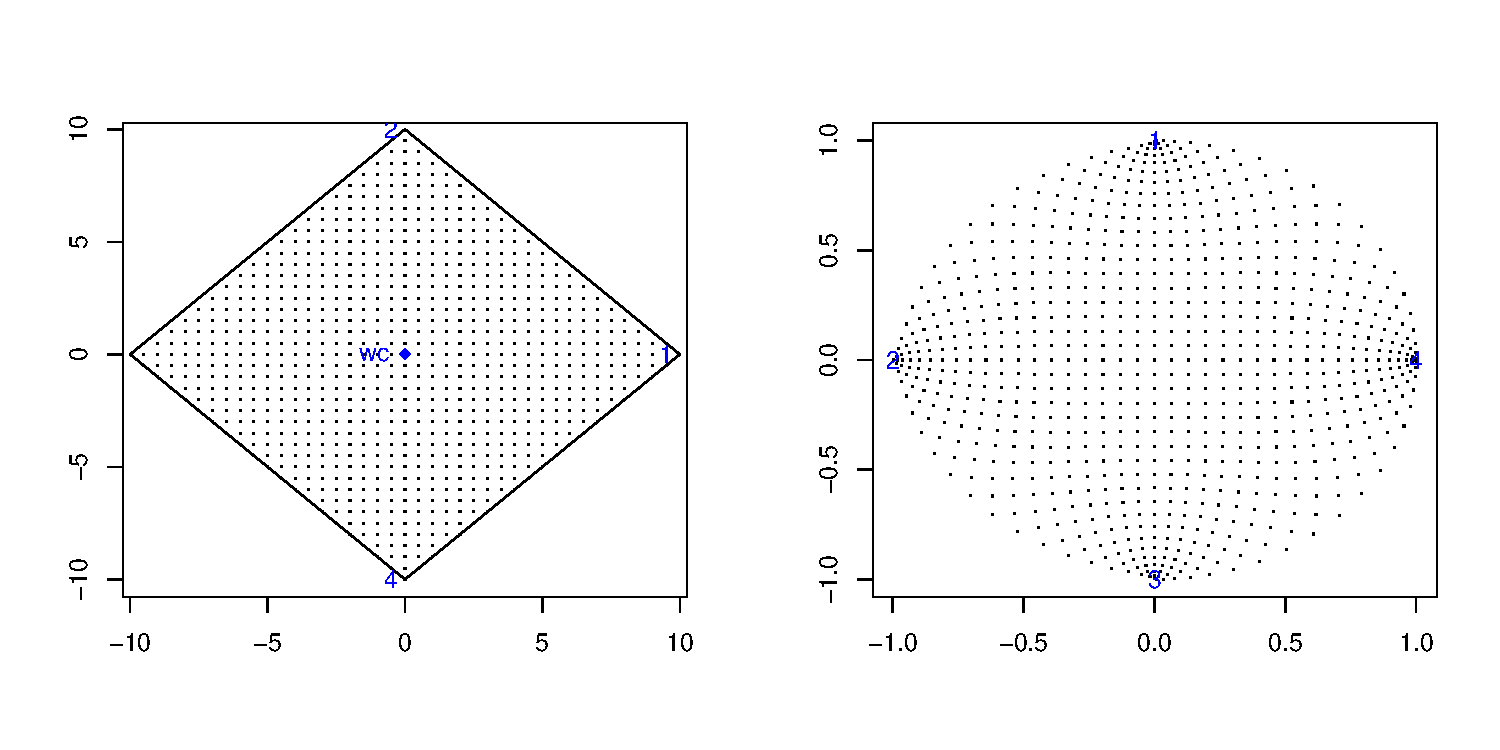
\includegraphics[scale=0.5]{sc/figs/squaredomain.pdf}
\caption{A regular grid of points over the square region (left). The right panel shows the mapping of these points under the \sch transformation to the unit disk.}
\label{squaredomain}
\end{figure}

% Irregular mapping diagram
\begin{figure} [tbp]
\centering
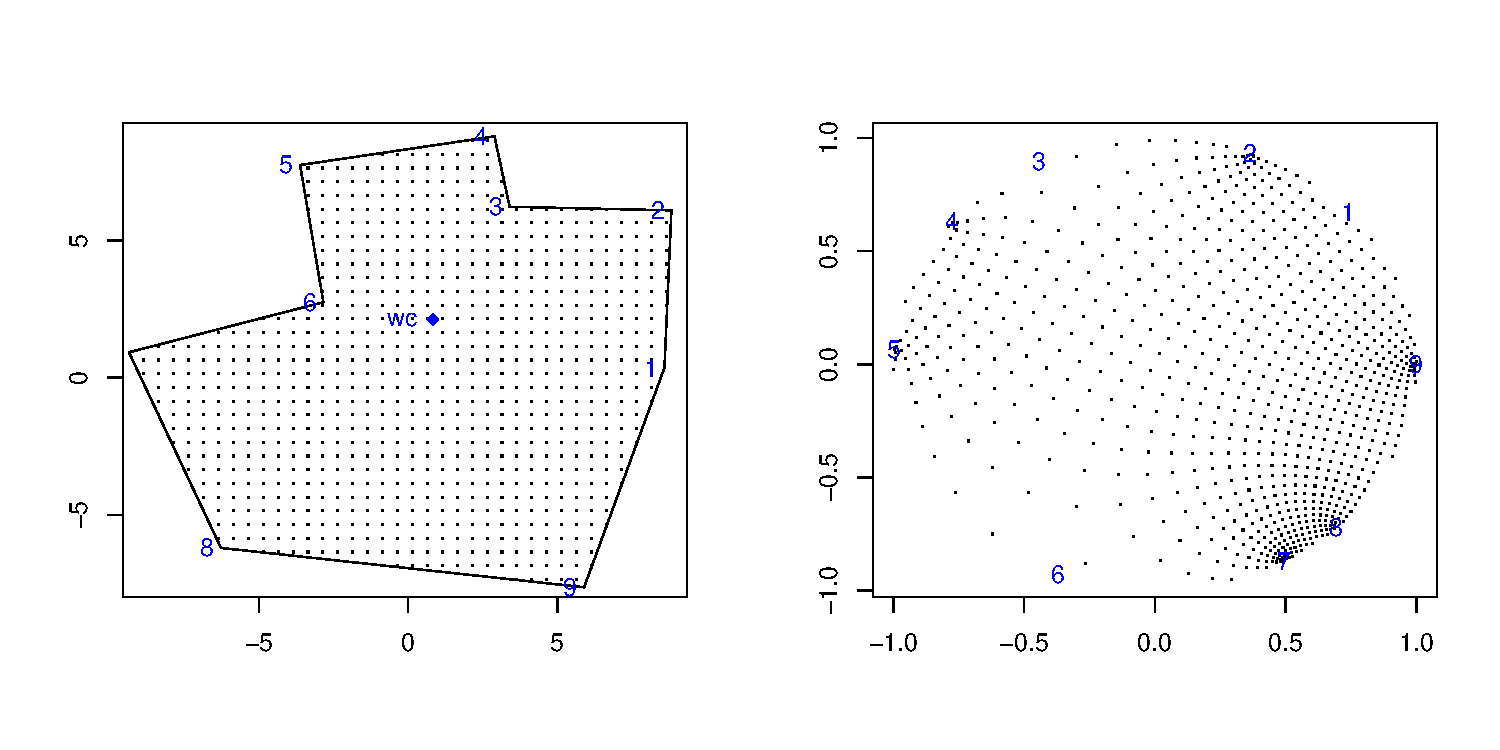
\includegraphics[scale=0.5]{sc/figs/irregulardomain.pdf}
\caption{A regular grid of points over region bound by a irregular nonagon (left). The right panel shows the mapping of these points under the \sch tranformation to the unit disk.}
\label{irregdomain}
\end{figure}

\subsection{Crowding}

\subsubsection{The crowding problem}
When the polygon is elongated or has many vertices, the mapped vertices may be positioned too closely in the transformed domain. This effect is referred to as \emph{crowding} and can be observed in \fig{crowdeddisk}. In elongated regions prevertices can be located exponentially close such that they are indistinguishable in finite precision arithmetic (\cite{howell90}).

% Crowded mapping diagram
\begin{figure} [tbp]
\centering
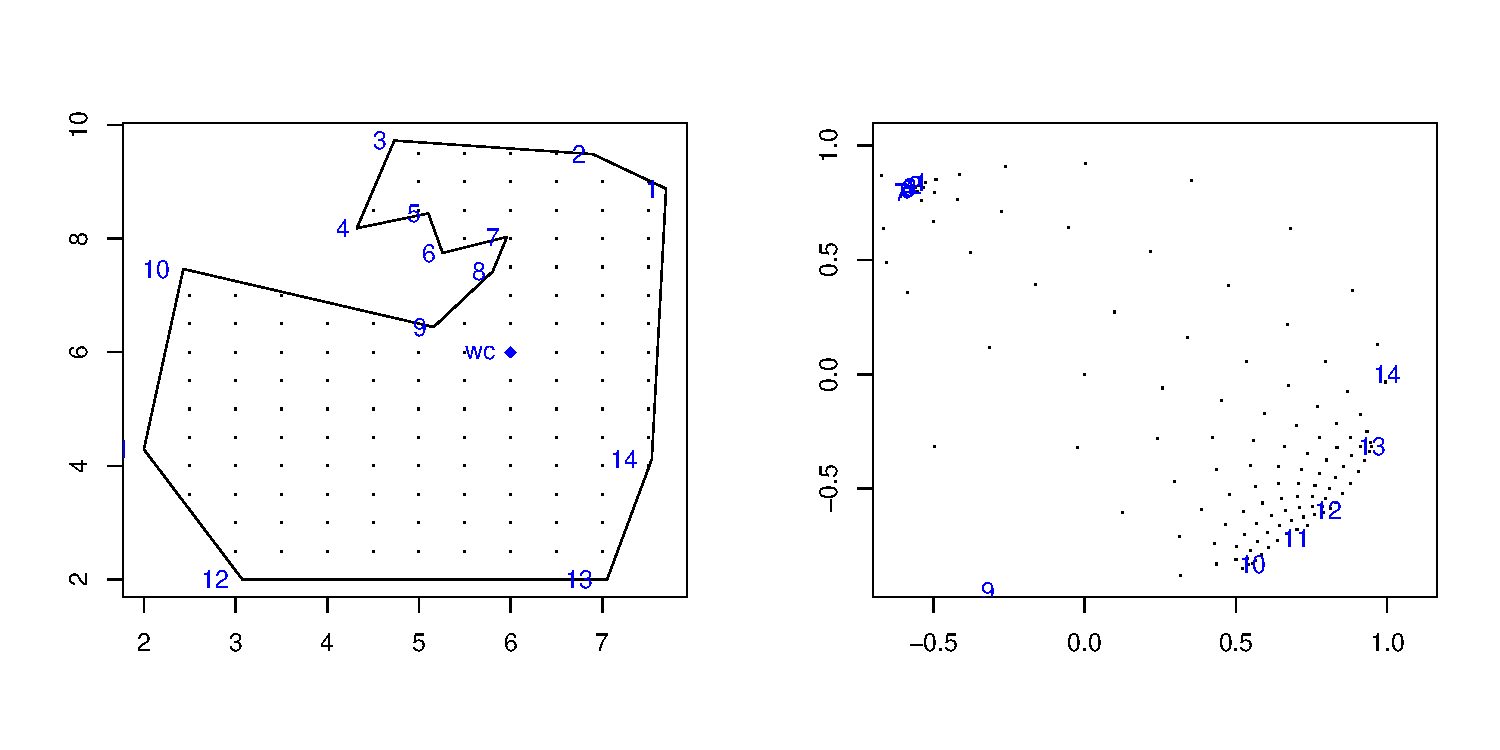
\includegraphics[scale=0.5]{sc/figs/crowdeddisk.pdf}
\caption{An example of crowding. Note that prevertices 1 through 8 are mapped almost to a singularity in the right panel.}
\label{crowdeddisk}
\end{figure}

\subsubsection{Fixing crowding}

If the crowding is caused by $\Gamma$ being elongated then a  primitive fix is to map to an elongated domain such as the rectangle or plane. This approach is suggested in \cite{howell90} however, as they point out, this does not eliminate all crowding and problems can still occur when there are strongly acute peninsulae in the polygon. Mapping to an elongated domain also does not fix problems which occur when mapping from T- or H-shaped domains (so-called ``multiply elongated'' domains).

In order to combat this problem more effectively, \cite{vavasis96} propose the CRDT (cross-ratios of the Delaunay triangulation) algorithm (see below). Each set of prevertices has $n-3$ degrees of freedom hence, there is a three parameter family of possible vertex arrangements that all map to the same polygon. The most stable of these \emph{embeddings} should be used. The M\"{o}bius transformation relates the embeddings to one another.

This idea can be extended by noting that the polygon is identical when additional vertices are added between the current ones, provided that the internal angle associated with the new vertex is $\pi$. These extra vertices also do not change the \sch formula since in \eqn{unitscmap} $\alpha_k=1$ for an angle of $\pi$. Adding these extra vertices allows us to control the aspect ratio of the mapping.

In the solution to the \sch parameter problem given in \secref{sc-parprob}, conditions on the side lengths and orientations of the polygon are enforced. The CRDT algorithm imposes conditions about quadrilateral sections of the polygon and the diagonals of the polygon. First a Delaunay triangulation of the domain is performed and then pairs of triangles are merged into quadrilaterals. A measure is then defined (the \emph{cross-ratio}) which specifies a set of non-linear equations to be solved. These equations enforce the constraint that the cross-ratio in mapped polygon comes out correctly. 

Putting all of these ideas together gives the CRDT algorithm (\cite{driscoll}, pp. 30-39). We first add edges to the polygon with internal angle $\pi$ to remove enlongated parts of the domain and then triangulate the domain. Once the domain is triangulated we find the cross-ratio:
\begin{equation}
\rho(a,b,c,d) = \frac{(d-a)(b-c)}{(c-d)(a-b)},
\end{equation}
for each of the $n-3$ quadrilaterals in the polygon (where $a,b,c,d$ are prevertices). Then, analogously to \eqn{optimizeme} we set up a series of equations, specifying that the cross-ratios remain the same in the polygon and the transform of the rectangle back to the polygon. We then wish to solve for the values of $\rho$ for the original domain in the same manner as we solved for side lengths in the original problem. 

In \fig{uncrowdeddisk} the CRDT method is used with a rectangular domain, crowding has been alleviated to some degree. The point density, as well as vertex density seems to be more uniform than in \fig{crowdeddisk}.

% Uncrowded mapping diagram
\begin{figure} [tbp]
\centering
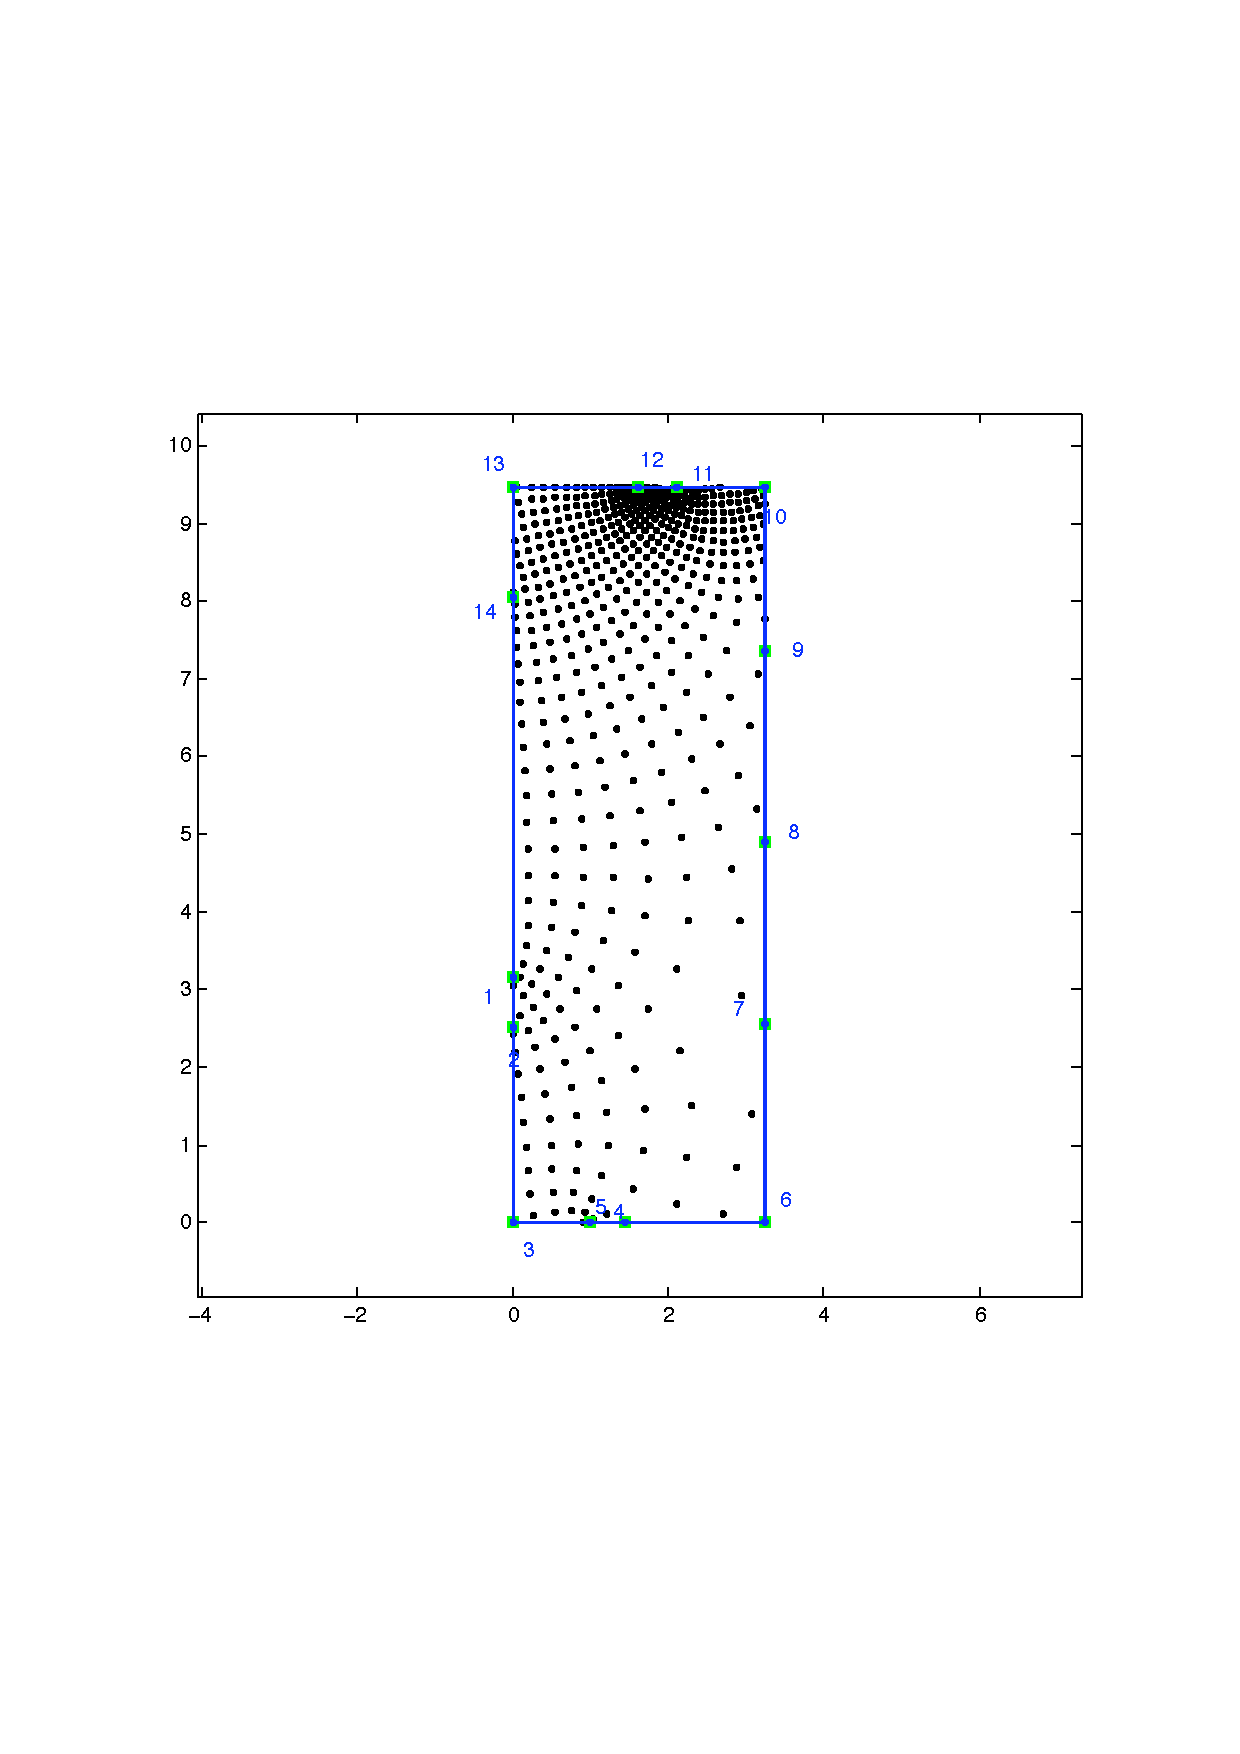
\includegraphics[scale=0.5]{sc/figs/irregular-fixed-crdt.pdf}
\caption{The mapping of the irregular domain featured in \fig{crowdeddisk} using the CRDT method mapping to a rectangle. The crowding is now much less severe.}
\label{uncrowdeddisk}
\end{figure}

The downside of using CRDT is that it may add too many vertices to maintain the aspect ratio, so the algorithm takes longer to run than the one specified in \secref{algorithmsketch} since it tends to be cubic in the number of vertices (\cite{driscoll05}). This is offset against the fact that the problem becomes tractable.

\section{Simulation experiments}

In order to test the efficacy of the \sch transform for the purposes of smoothing over complex regions, a series of simulation experiments were performed. The \emph{SC Toolbox} for MATLAB was used to perform the transform and the mapping of the points. These were then fed into \textsf{R} and models run using packages \texttt{mgcv} and \texttt{soap}.

\subsection{Ramsay horseshoe}

The most obvious candidate for simulation is the Ramsay horseshoe (see \secref{ramsayfunc}). In order to map the horseshoe, we first draw a rough bounding box around the shape. In order to map as simple a domain as possible, to begin with a bounding box was used as the $W$ domain remapped via the \texttt{evalinv()} function from the \emph{SC Toolbox}. This is shown in \fig{hswithboundingbox}. The bounding box is then transformed to the rectangle. 

\begin{figure}
\centering
% trim order l b r t
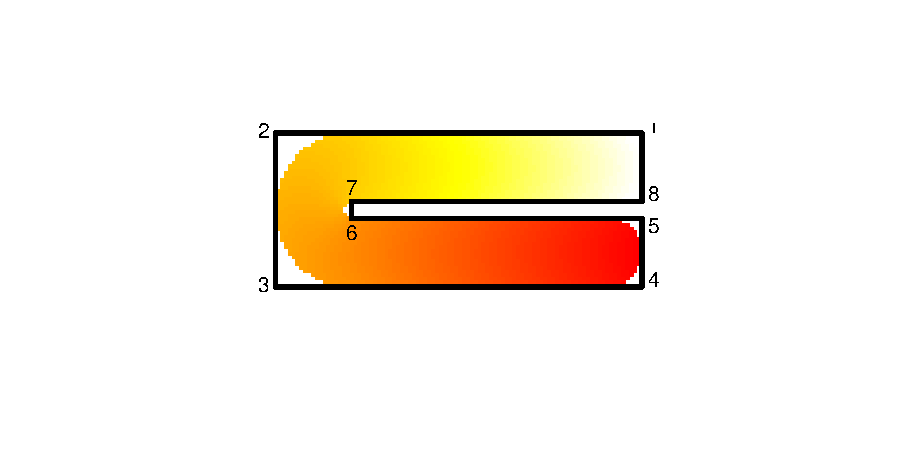
\includegraphics[trim=0.5in 1in 0in 0.5in]{sc/figs/hswithboundingbox.pdf} \\
\caption{The horseshoe with its bounding box. The vertices marked 1, 4, 5 and 8 are mapped to the corners of the rectangle.}
\label{hswithboundingbox}
% generated by /phd-smoothing/sc-writeup/figs/hswithboundingbox.R
\end{figure}

A sample of 1000 points was then taken from the horseshoe and noise added to the data. First the $x$,$y$ coordinates of the sampled points were expressed as complex numbers of the form $w=x+iy$. The sample was then mapped into $W^*$, creating a new set of coordinates $w^*=x^*+iy^*$. Smoothing was then performed over the responses in the $W^*$ domain using the \texttt{gam()} function in \texttt{mgcv}. 

\begin{figure}
\centering
% trim order l b r t
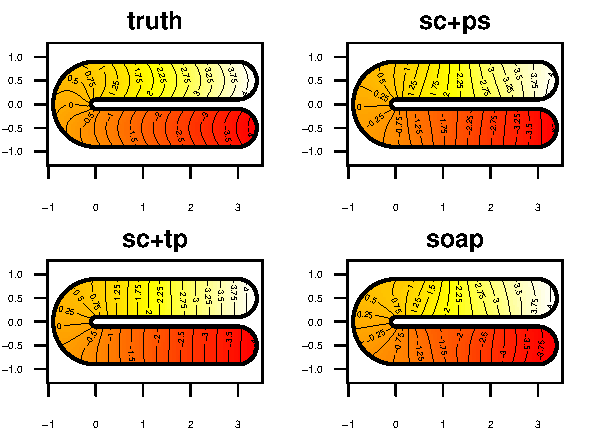
\includegraphics[width=4in]{sc/figs/compsmooth.pdf} \\
\caption{A typical set of predictions using P-splines on the transformed domain (top right), thin plate splines on the transformed domain (bottom left) and soap film smoother (bottom right) for the Ramsay horseshoe (top left). Sample size was 250, noise level was set to $\sigma=1$.}
\label{compsmooth}
% generated by figs/pspline.soap.comp.hs.R
\end{figure}

\Fig{compsmooth} shows the true function and typical realisations of: the fit given by a \tprs on the transformed domain, a P-spline fit on the transformed domain and the fit given by the soap film smoother. Looking at the heat maps one can see that the general shape of the horseshoe function is clearly being reproduced by all methods (especially in comparison to that in \fig{leakage}). However, on the transformed domains the curvature across the minor axis is not being captured.

\begin{table}[tb]
\begin{tabular}{c c}\\
Sample size & Noise level \\
\hline
\hline
1000 & 0.3 \\
500 & 0.3 \\
250 & 0.3 \\
100 & 0.3 \\
1000 & 0.5 \\
1000 & 1 \\
1000 & 2 \\
\end{tabular}
\caption{Setup for the simulations using the \sch transform for the Ramsay horseshoe. Noise level ($\sigma$) is the number a random deviate from a standard Normal distribution was multiplied by before being added to the true test function.}
\label{scramsimtable}
\end{table}

\Tabref{scramsimtable} shows the settings for noise level and sample size of the simulations. Mean squared error between the true function and the fitted model was used to evaluate the performance of the models. In the following tables we provide the mean squared error over a prediction grid of 1000 points averaged over 1000 generated data sets. The fits on the transformed domain and the soap film have much smaller MSE than the thin plate spline, except in one case, \sch with P-splines for sample size 100 and noise level 0.3. Looking closer at the results for this model, there were two results where the MSE was 54.68 and 437.99 which, when removed, put the MSE back to 0.03003, which seems much more reasonable. These results were presumably due to the P-splines having the same knot setup for each realisation, giving a poor model when there was not enough data. This shows one of the many disadvantages of a knot-based approach.

\begin{figure}
\centering
% trim order l b r t
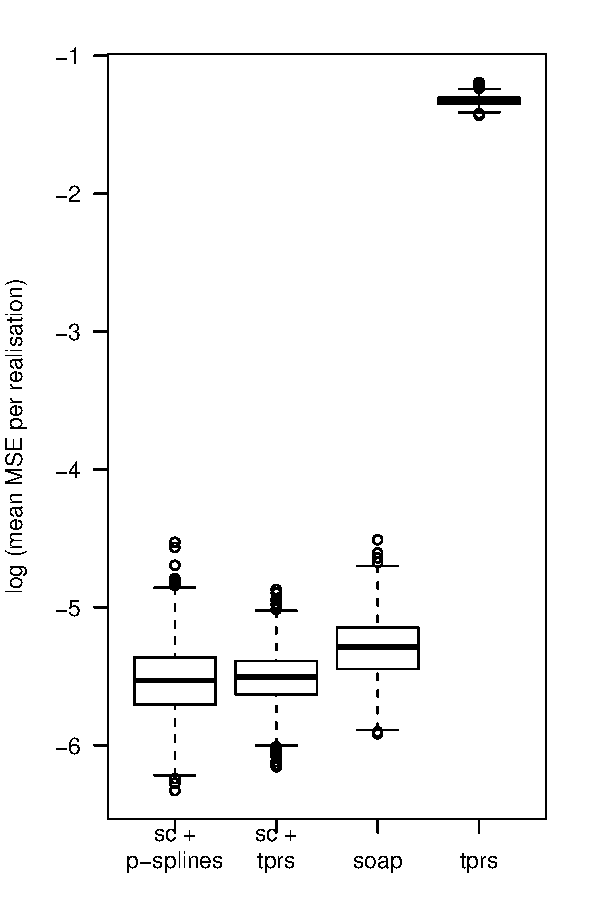
\includegraphics{sc/figs/sc-mses-boxplot.pdf} \\
\caption{Boxplots of mean MSE from 1000 points on a prediction grid from 1000 simulations for the Ramsay horseshoe. Models fitted were \sch transform with P-splines and \tprs, the soap film smoother, and \tprs (with the untransformed domain). Error level was set to 0.3.}
\label{scram1000boxplots}
% generated by sc/figs/makeboxplots.R
\end{figure}

\begin{table}[ht]
\begin{tabular}{c c c c c c}\\
& & & MSE (se) &\\
Sample size & Noise level & TPRS & SC + P-spline& SC + TPRS & Soap film\\
\hline
\hline
%1000 & 0.3 & 0.00412 (0.00112) & 0.00811 (0.00243) & 0.00517 (0.00114) \\ 
%500 & 0.3 & 0.00505 (0.00144) & 0.00478 (0.000955) & 0.00628 (0.00146) \\ 
%250 & 0.3 & 0.00875 (0.00392) & 0.00684 (0.00183) & 0.0107 (0.00305) \\ 
%100 & 0.3 & 0.0225 (0.035) & 0.0118 (0.00461) & 0.0219 (0.0117) \\ 
%1000 & 0.5 & 0.0105 (0.00353) & 0.00811 (0.00243) & 0.0127 (0.0034) \\ 
%1000 & 1 & 0.0242 (0.0108) & 0.0161 (0.0069) & 0.0275 (0.00958) \\ 
%1000 & 2 & 0.066 (0.0481) & 0.0388 (0.0229) & 0.0686 (0.0333) \\ 
1000 & 0.3 & 0.26611 (0.00029) & 0.00412 (4x10$^{-5}$) & 0.00811 (8x10$^{-5}$) & 0.00517 (4x10$^{-5}$) \\ 
500 & 0.3 & 0.28276 (0.00083) & 0.00505 (6x10$^{-5}$) & 0.00478 (4x10$^{-5}$) & 0.00628 (7x10$^{-5}$) \\ 
250 & 0.3 & 0.32274 (0.00268) & 0.00875 (0.00025) & 0.00684 (0.00012) & 0.01073 (0.00019) \\ 
100 & 0.3 & 0.48371 (0.01765) & 0.52264 (1.39562) & 0.01178 (0.00046) & 0.02194 (0.00117) \\ 
1000 & 0.5 & 0.27336 (0.00032) & 0.01055 (0.00011) & 0.00811 (8x10$^{-5}$) & 0.01268 (0.00011) \\ 
1000 & 1 & 0.30718 (0.00056) & 0.02422 (0.00034) & 0.01607 (0.00022) & 0.02749 (3x10$^{-4}$) \\ 
1000 & 2 & 0.42296 (0.00144) & 0.06596 (0.00152) & 0.03875 (0.00072) & 0.06859 (0.00105) \\ 
\end{tabular}
\label{scramsayres}
\caption{Mean squared error along with its standard error for the transformed Ramsay horseshoe (for P-spline and thin plate cases) versus those for the soap film smoother. See below for information on the asterisked result.}
% generated by /phd-smoothing/sc-writeup/tablecode/ramsay.sim.results.table.R
\end{table}

\Tabref{scramsayres} shows the results from the simulations for the horseshoe. The \sch transform yields results which are comparable, it not better, than the soap film. Once we get to 100 samples the method performance degrades over all methods. Although this seems initially encouraging, it is worth bearing in mind at this point that in domains like the horseshoe it is obvious what the transform should be.

Indeed, this can be seen by looking at the predicted values for the model in the $W^*$ domain. \Fig{hsvisgam} shows predictions from the fitted surface alongside the true values when the domain has been put into its ``natural'' coordinate system. The coordinate system for the fitted values is the \sch transformed system and for the true values the system is the major and minor axes of the shape (ie. one axis along the central curve of the shape and the other perpendicular to that). In the plot, the strong linear trend along the major axis of the horseshoe can be seen in both cases, making this a rather trivial smoothing problem. The smooth is being calculated in a close approximation to its natural domain. Such an approximation would not be as easy to find for a less regular, more realistic domain.

\begin{figure}
\centering
% trim order l b r t
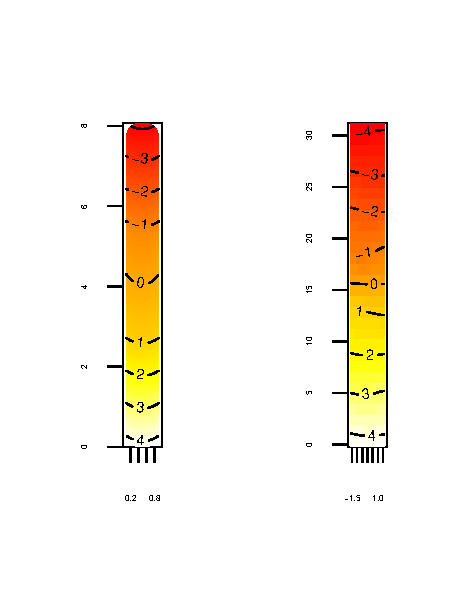
\includegraphics[trim=0in 0.5in 0in 0in]{sc/figs/hsvisgam.pdf} \\
\caption{Heatmap of the true values of the modified Ramsay horseshoe projected into its natural domain (left) and the predicted values of the fit given using the \sch transform and then smoothed using a \tprs (right).}
\label{hsvisgam}
% generated by /phd-smoothing/thesis/sc/figs/hsvisgam.R
\end{figure}

\subsubsection{Alternate Ramsay horseshoe}

The second domain tested was the alternate version of the Ramsay horseshoe from \cite{soap}. For this domain the gradient runs across the short axis of the horseshoe (see \fig{altramsayhorseshoe}). The same simulation setup was used as for the first domain.

\begin{figure}
\centering
% trim order l b r t

\includegraphics[trim=0.5in 1in 0in 0.5in]{sc/figs/altramsayhorseshoe.pdf} \\
\caption{Heatmap of the alternate version of the Ramsay horseshoe.}
\label{altramsayhorseshoe}
\end{figure}

For the alternative horseshoe we begin to see the soap film creep ahead of the transformation method (see \tabref{scaltramsayresultstable}). Although the MSEs are of approximately the same order (as are the standard errors), the soap film is gaining ground. 


To examine what is going on here we can look at the plots of the predicted values as heat maps. These can be seen in \fig{altramsaycomp} and show that the \sch mapping seems to capture the overall structure of the shape better than the soap film smoother, which seems to capture patches of the shape but not the overall structure. It also appears that the \sch method does not respect the ends of the horseshoe and continues the gradient running along the minor axis over this part as well.This feature seems to be the cause of the performance decrease.

------------------------


\begin{table}[ht]
\begin{tabular}{c c c c c c}\\
& & & MSE (se) &\\
Sample size & Noise level & TPRS & SC + P-spline& SC + TPRS & Soap film\\
\hline
\hline
%1000 & 0.3 & 0.00415 (0.00117) & 0.0158 (0.00247) & 0.00378 (0.00108) \\ 
%500 & 0.3 & 0.00469 (0.00147) & 0.00793 (0.00186) & 0.00458 (0.00145) \\ 
%250 & 0.3 & 0.00716 (0.00431) & 0.0142 (0.00249) & 0.00771 (0.00301) \\ 
%100 & 0.3 & 0.039 (0.22) & 0.0201 (0.00589) & 0.0298 (0.42) \\ 
%1000 & 0.5 & 0.00839 (0.00403) & 0.0158 (0.00247) & 0.00966 (0.00371) \\ 
%1000 & 1 & 0.0194 (0.0122) & 0.0226 (0.0085) & 0.019 (0.00981) \\ 
%1000 & 2 & 0.0605 (0.0468) & 0.0436 (0.0276) & 0.041 (0.0434) \\ 
1000 & 0.3 & 0.0109 (8x10$^{-5}$) & 0.00415 (4x10$^{-5}$) & 0.01579 (8x10$^{-5}$) & 0.00378 (3x10$^{-5}$) \\ 
500 & 0.3 & 0.01395 (1x10$^{-4}$) & 0.00469 (7x10$^{-5}$) & 0.00793 (8x10$^{-5}$) & 0.00458 (6x10$^{-5}$) \\ 
250 & 0.3 & 0.01721 (2x10$^{-4}$) & 0.00716 (0.00027) & 0.01418 (0.00016) & 0.00771 (0.00019) \\ 
100 & 0.3 & 0.0229 (0.00099) & 0.03904 (0.02197) & 0.02011 (0.00059) & 0.02975 (0.04195) \\ 
1000 & 0.5 & 0.01521 (6x10$^{-5}$) & 0.00839 (0.00013) & 0.01579 (8x10$^{-5}$) & 0.00966 (0.00012) \\ 
1000 & 1 & 0.02084 (0.00023) & 0.01943 (0.00038) & 0.02264 (0.00027) & 0.01902 (0.00031) \\ 
1000 & 2 & 0.03843 (0.00072) & 0.06053 (0.00148) & 0.04363 (0.00087) & 0.04096 (0.00137) \\ 
\end{tabular}
\label{scaltramsayresultstable}
\caption{Mean squared error along with its standard deviation for the transformed alternate Ramsay horseshoe (for P-spline and thin plate cases) versus those for the soap film smoother.}
% generated by /phd-smoothing/sc-writeup/tablecode/alt.ramsay.sim.results.table.R
\end{table}

\begin{figure}
\centering
% trim order l b r t
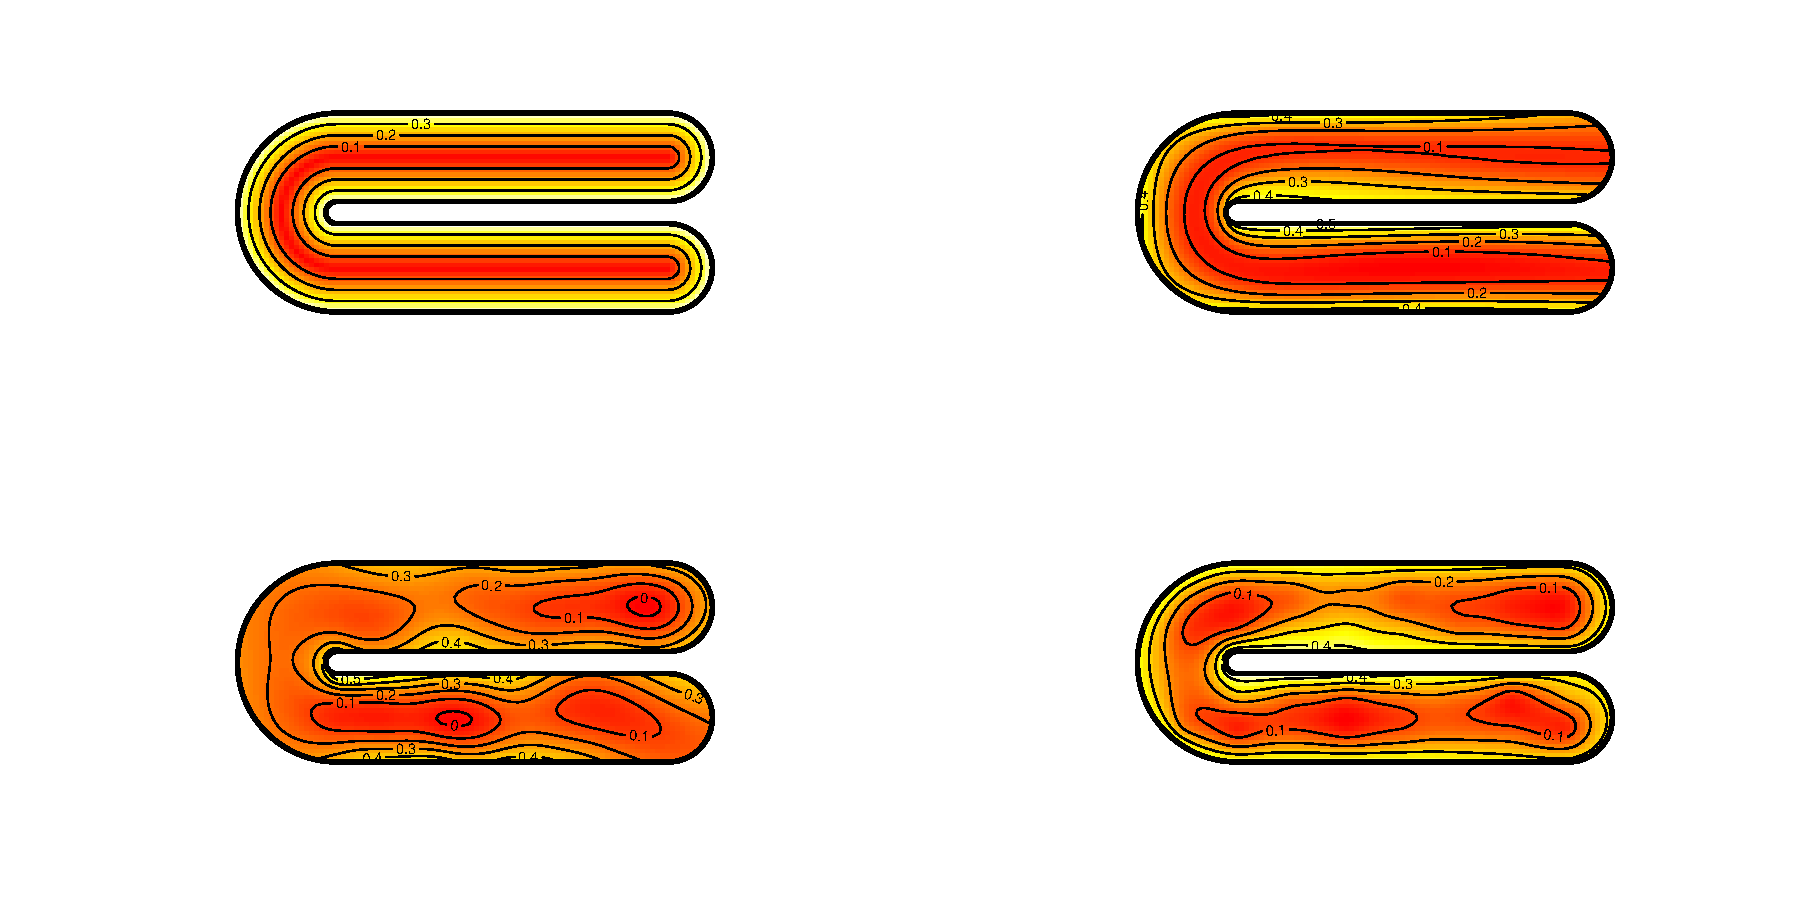
\includegraphics[width=4in]{sc/figs/altramsaycomp.pdf}\\
\caption{Single realisations of the fit to the alternate Ramsay horseshoe for each method. Clockwise from top left: the original figure, the function estimated by the \sch transform with P-splines, function estimated by the \sch transform with thin plate splines and finally the soap film estimate. Error set to $\sigma=1$.}
\label{altramsaycomp}
% generated by /phd-smoothing/sc-writeup/figs/altramsaycompare.R 
\end{figure}


\subsubsection{What's happening?}

At this point it is useful to get an idea about what the transformation is doing to the domain, specifically to find out about the distortion to space caused by the transform. To investigate this we can take a straight line in the $W$ domain and see what it maps to in the $W^*$ domain. We can also look at the response along that line according to the transformed and untransformed coordinate systems and see how this compares to looking at the response in the horseshoe's natural coordinate system.

\begin{figure}
\centering
% trim order l b r t
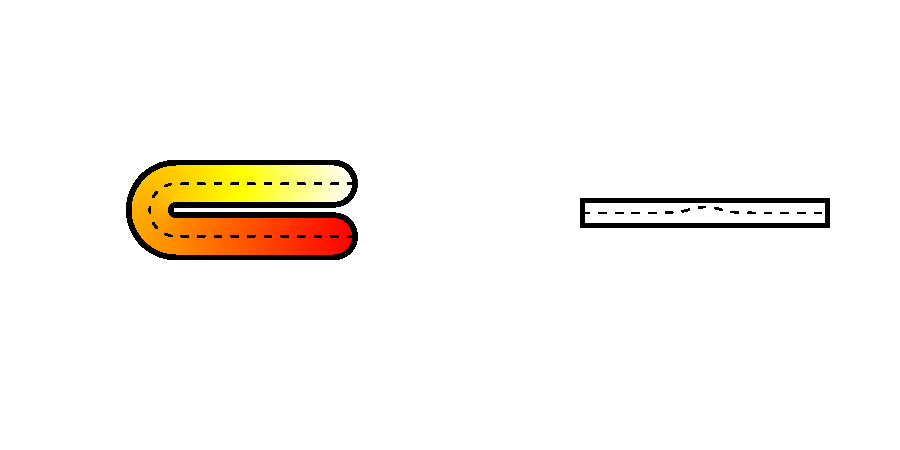
\includegraphics[trim=0.5in 1in 0in 1in]{sc/figs/horseshoecentreline.pdf} \\
\caption{Mapping of a straight line along the major axis of the Ramsay horseshoe to its position in the ``unwrapped'' domain.}
\label{horseshoecentreline}
% generated by /phd-smoothing/ramseysim/nullspace.test.R 
\end{figure}

\Fig{horseshoecentreline} shows the line that was evaluated along the centre of the horseshoe and its equivalent line in the transformed domain. We can see from this that a line that is straight in the domain appears to be bent in the transform. The curvature does not appear to be particularly extreme in this case, however, one can imagine that this could get significantly worse for regions with more complicated boundaries. Although this is interesting, it is more revealing to look at the evaluations of the horseshoe functions along that line.

\Fig{centrelinelineplot} shows the evaluations of the horseshoe function over the line plotted against three coordinate systems. The first plot shows the function evaluations on the $W$ domain as a response to change in $y$. The second on the $W^*$ domain, as a response to $y^*$, in the transformed coordinate system. The final plot is in the horseshoe's ``natural'' domain, \emph{ie.} the value the horseshoe takes as a function of distance along the major axis of the shape. From these plots one can see the quality of approximation to the natural domain of the horseshoe the \sch transform affords. Only two minor kinks occur in the line. Looking at where the kinks occur, they correspond exactly to those kinks in \fig{horseshoecentreline}. This makes sense, since we would expect a change in gradient if direction we are traveling has moved into two dimensions from one.

\begin{figure}
\centering
% trim order l b r t
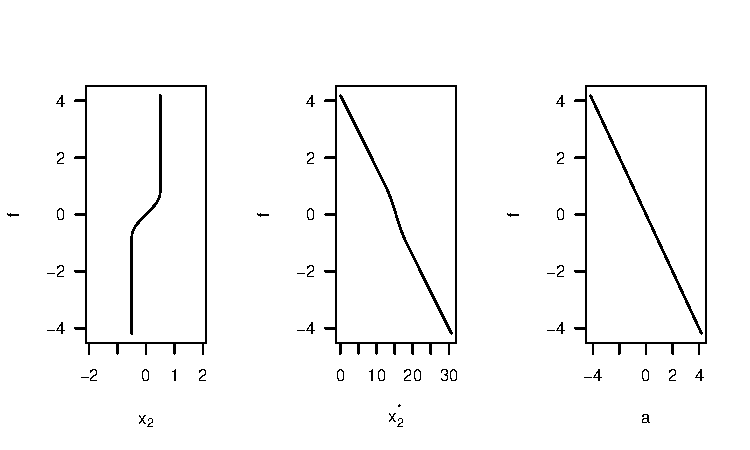
\includegraphics[trim=0in 0in 0in 0in]{sc/figs/centrelinelineplots.pdf} \\
\caption{Plots of the horseshoe function against the $y$ axis for (left) the untransformed horseshoe, (middle) the shape under the \sch transform and, (right) the function evaluation against the major axis.}
\label{centrelinelineplot}
% generated by /phd-smoothing/ramseysim/nullspace.test.R 
\end{figure}


\Fig{altcentrelinelineplot} shows analogous plots to \fig{centrelinelineplot} and backs up this hypothesis. The second panel shows the mapping of the $y$ component of the centreline against the response and the third panel shows the same in the horseshoe's own domain. The two plots appear to be indistinguishable.

\begin{figure}
\centering
% trim order l b r t
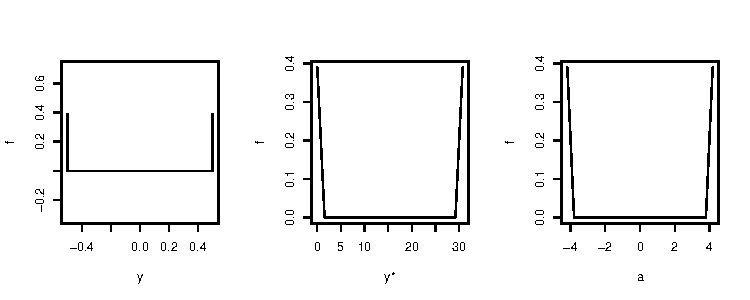
\includegraphics[trim=0in 0in 0in 0in]{sc/figs/altcentrelinelineplots.pdf} \\
\caption{Plots of the alternate horseshoe function against the $y$ axis for (left) the untransformed horseshoe, (middle) the shape under the \sch transform and, (right) the function evaluation against the major axis.}
\label{altcentrelinelineplot}
% generated by /phd-smoothing/altramsaysim/nullspace.test.R 
\end{figure}



\section{Conclusions \& Analysis}

This brief foray into conformal mapping has provided plenty of insights into how smoothers will act under mapping schemes. It also gives insight into which criteria are useful for a transformation-based method. For example, the angle-preserving properties of the \sch transform are of little use in a smoothing context. It is also clear that a method that does not produce crowding-type phenomena is desirable. These examples show the serious disadvantages of the approach, the ability of the transform to clearly split the domain and truly separate those parts interfering with one another is very useful.

Although the \sch transform is rather disappointing in practice, it does show that a mapping-type technique can produce some reliable results, even if it is on a limited number of domains. In essence the main downfall of the \sch transform is that it re-maps the domain too rigidly. There is no flexibility to the domain into which one is mapping, it must be one of those detailed above. It is now clear that such an inflexible strategy will not yield good results in all situations and, indeed, there are a limited number of situations in which such an approach will be useful.



\chapter{Multidimensional scaling for domain-dependent finite area smoothing}

% MDS stuff

\label{chap-mds}

\section{Introduction}

Following the work of the previous chapter, the objective is now to find a mapping of the data into a new space which causes minimum distortion to the points in that new space. At the same time the mapping must also effectively separate those parts of the original domain which are subject to leakage. This balance (between making sure the model overcomes leakage whilst at the same time does not cause artefacts in the smooth) is essential to the success of the approach. The \sch\ transform approach, of dictating the transformed domain from the outset is clearly not flexible enough for general use, however a method that depends on the shape of original domain may have more promise.

\subsection{Proposition}

Multidimensional scaling (MDS) or, as it is often referred to, principle coordinates (PCO) (\cite{gower1966}) is a method used in multivariate analysis. It is closely related to techniques such as PCA (\cite{chatfieldcollins}, p. 200) and canonical correspondence analysis (\cite{terbraak}). The starting point for MDS is a matrix of distances, representing some kind of dissimilarity between observations. This distance could be calculated from the data, for example ideological distance between politicians measured using NOMINATE scores (\cite{quantss}, p. 225), or could instead be distances that occur in the data naturally through experimental setup,  for example comparative distances between stimuli response in a psychophysical experiment (\cite{torgerson}). Here we concentrate on geographical distances.

MDS takes this matrix of distances and projects the data in such a way that Euclidean inter-point distances in the projection are approximately the same as the distances in the matrix (\cite{chatfieldcollins}, p. 187). If the matrix of distances is of rank $m$ then the projection can be in $m-1$ or less dimensions; a projection into 2 dimensions is a typical choice, since it is easily visualised. For this reason one can also think of MDS as a dimension reduction technique, finding a projection of a data cloud into lower dimensional space, while still retaining information about the dissimilarities between the points.

When MDS is performed on some categorised set of dissimilarities (as is often the case in social science and psychology) it is referred to as non-metric MDS, where as on a continuous scale it is known as metric MDS. Though they have different names, the calculations are identical (aside from the method of finding the distances). Discussion here will focus on metric MDS.

Multidimensional scaling offers a framework for finite area smoothing over a region with a complex boundary. Given the set of distances between points in a domain, we can project those points into a configuration such that the distances between those points are approximately preserved. Now, if the Euclidean metric were to be used to calculate the distances between the points then the result from the projection would be identical to the starting point configuration (provided that we projected back into the same number of dimensions). However, if it were possible to use a metric that took into account the distance within the boundary (a within-area distance) then the resulting configuration of points would (approximately) respect the boundary of the domain.

Justification for this approach is as follows. In many applications within-area distances is meaningful, given that there is some reasoning behind why certain parts of the domain should not affect one another. Biological populations respect the intrinsic structure of these domains and in general do not respect Euclidean geometry in their movement patterns (for example, they move around obstacles, avoid predators and track prey). When within-area distances are meaningful, it makes sense to use this information about the structure of the domain rather than somewhat arbitrarily choose Euclidean geometry and discard this extra informaton. However, as literature on smoothing is firmly based in a Euclidean context, it would be preferable to perform the smoothing in Euclidean space. In this case the approximation to Euclidean space afforded by an MDS projection of the within-area distances offers a bridge between these two requirements.

\subsection{Procedure}
\label{mdsproc}
Given a sample $\{\bm{x}_i, z_i : i=1\dots n\}$, the set of points in the domain over which smoothing is to be performed, $\bm{x}_i$ is the location (a $k$-vector, although here 2-vectors are assumed throughout) of the $i^\text{th}$ point with response $z_i$ (assumed to be univariate). Here, finding an MDS configuration of a set of points consists of: $i$) calculating the within-area distances between the points, $ii$) forming the distance matrix and, $iii$) actually performing the MDS projection.

The whole proposed procedure is as follows:

\begin{enumerate}
\item Obtain the MDS configuration for the domain using some representative set of points over the area in question. The only use of the MDS locations obtained in this step is to find the initial MDS configuration; they are discarded afterward. Representative points could be a sparse grid over the domain or a subset of $\{\bm{x}_i : i=1\dots n\}$. More detail and justification is provided in \secref{grids}, below.

\item Using the MDS configuration obtained above along with Gower's interpolation (see \secref{gowers}) to obtain the location of the sample in the MDS configuration: $\{\bm{x}_i^*, z_i : i=1\dots n\}$.

\item Smooth $\{\bm{x}_i^*, z_i : i=1\dots n\}$ using a penalised regression spline.

\item To predict at a location $\bm{x_j}$ in the original domain, use Gower's interpolation to obtain the point's location in the MDS space: $\bm{x}_j^*$. Predict $\hat{z}_j$ at $\bm{x}_j$ using the smooth at $\bm{x}_j^*$.
\end{enumerate}

This approach is referred to as \mdsap\ (MultiDimensional Scaling with Regression Splines) throughout the chapter.

The rest of this chapter is structured as follows: in \secref{MDStechdet} a technical overview of MDS is given, along with technical details of how the MDS configuration is calculated; \secref{mdsdist} focuses on how the within-area distances are found; \secref{mdssims} shows some examples of this method on simulated data. \Secref{MDSimprov} shows some improvements to the initial method and further simulations, \secref{mds-problems} details remaining problems and \secref{mds-prac} gives some notes for practitioners wishing to use \mdsap. Finally, \secref{mds-conc} draws the topic to a conclusion and lays out areas of further work and interest.


\section{Technical details}
\label{MDStechdet}

The basic concept behind MDS as used here is to take the data, calculate their within-area inter-point distances and then find their points in a new coordinate system based on those inter-point distances. Their new positions are determined by finding the eigen-decomposition of the (centred) matrix of distances between points. First a description of the MDS procedure when Euclidean distances are used is given, followed by the justification for the use of the same procedure when using within-area distances. 

\subsection{Finding the new point configuration}

First define $d_{ij}$ as the distance between the points $i$ and $j$. These are used to form a (symmetric) matrix, $D$, with \ijth element $d^2_{ij}$. For the moment let us assume that $D$ is known and $d_{ij}$ is the Euclidean distance between points $i$ and $j$. 

\cite{diaconis08} gives a clear definition of the algorithm (due to \cite{schoenberg35} and \cite{torgerson}) for finding the new locations of points, which is outlined below. Further detail is given in \cite{principlesofMA}, pp. 104-108 and \cite{chatfieldcollins}, pp. 189-200.

First, suppose that the $n$ unknown new locations (in $n$ dimensions) in our MDS configuration are rows of an $n \times n$ matrix, $\tilde{X}^*$. Now let $S=\tilde{X}^{*} \tilde{X}^{*\text{T}} $, so $S$ is a matrix of scalar products of the point vectors, \emph{ie.} the \ijth element of $S$ is:
\begin{equation}
s_{ij} = \bm{x}_i\tr{\bm{x}_j},
\label{selem}
\end{equation}
$S$ is an $(n\cross n)$ matrix. Note that we may only find $\tilde{X}^*$ up to a translation and rotation, so it is assumed that the values in $\tilde{X}^*$ have been centred about the origin.

We now wish to relate $D$ to $S$. First, note that that \ijth element of D is 
\begin{equation}
d_{ij}^2 = (\bm{x}_i-\bm{x}_j)\tr{(\bm{x}_i-\bm{x}_j)} = \bm{x}_i\tr{\bm{x}_i} + \bm{x}_j\tr{\bm{x}_j}  -2 \bm{x}_i\tr{\bm{x}_j}.
\label{dij}
\end{equation}
Using \eqn{selem}, we can re-write \eqn{dij} as
\begin{equation}
D=\bm{s}_\text{diag}\tr{\bm{1}} + \bm{1}\tr{\bm{s}_\text{diag}} -2S.
\label{dijmat}
\end{equation}
where $\bm{1}$ is an $n \cross 1$ vector of 1s and $\bm{s}_\text{diag}$ is the $n \cross 1$ vector of diagonal elements of $S$.

Define:
\begin{equation}
H = I-\frac{1}{n}\bm{1}\tr{\bm{1}},
\end{equation}
where $I$ is the identity matrix, as usual, and $\bm{1}\tr{\bm{1}}$ is an $n \cross n$ matrix of 1s.

By pre- and post-multiplying any matrix by $H$ the matrix is double centred (such that row and column means are 0). Pre- and post-multiplying \eqn{dijmat} by $H$ yields:
\begin{equation}
HDH = -2HSH.
\end{equation}
The first two terms in on the right hand side of \eqn{dijmat} are zero since the rows of $\bm{s}_\text{diag}\tr{\bm{1}}$ and the columns of  $\bm{1}\tr{\bm{s}_\text{diag}}$ are constant. Since $S$ is already centred so $HSH=S$. Rearranging, the following relation between $S$ and $D$ holds:
\begin{equation}
S = -\frac{1}{2}HDH.
\end{equation}

Now there is a relation between $D$ and $S$, we can concentrate on dealing with $S$. In order to find $\tilde{X}^{*}$ we must factor $S$. There are many options for matrix decomposition. One option for factoring $S$ is to use the Cholesky decomposition, however, with MDS we are looking to decompose the space based on the directions of largest variation, \emph{ie.} those that have the largest contribution to $s_{ij}$. For that reason we use the eigen-decomposition.

Finding the eigen-decomposition of $S$, we obtain $S=U\Lambda\tr{U}$. Here $U$ is the $n \cross n$ orthogonal matrix of eigenvectors and $\Lambda$ is the $n \cross n$ diagonal matrix of eigenvalues. Then an $\tilde{X}^*$ satisfying \eqn{selem} may be computed as:
\begin{equation}
\tilde{X}^*=U\Lambda^{\frac{1}{2}}.
\end{equation}

Following these steps $\tilde{X}^*$ is an $n \cross n$ matrix. The aim here is to smooth in two dimensions, and in general multidimensional scaling is performed to reduce the dimensionality of the data, so we must now reduce the dimensionality of $\tilde{X}^*$. To represent the space using two dimensions the directions with the two largest eigenvalues are chosen and the others discarded. These two largest eigenvalues and their associated eigenvectors constitute the two largest sources of variation in distance (since they are the two largest contributions to $S$) this gives the two dimensional representation of the data. 

Defining $X^*$ to be the $n \cross 2$ dimensional matrix obtained from truncating the full new coordinate set to the first two columns in decreasing eigenvalue order, a 2-dimensional representation has been obtained. More generally, we can find the $k$-dimensional MDS representation of the space by just taking the first $k$ columns of $\tilde{X}^*$.

In summary, to calculate the MDS configuration of a set of points (given their inter-point distances) we merely need to double centre the matrix of distances, perform an eigen-decomposition on the resulting matrix, and finally truncate that matrix to the first $k$ columns.

For finite area smoothing, $d_{ij}$ should be the shortest distance between the points, given the path between any pair of points remains within the domain. Calculation of the inter-point distances is covered in \secref{mdsdist}, however it is important to first justify the use of these steps when non-Euclidean distances are used. 

One can think of the justification in the following way: given that the distances in $D$ obey the triangle inequality, all of the points in $D$ ($n$ of them if $D$ is $n \cross n$) may be represented by MDS in $n$ dimensional Euclidean space (at worst). Hence, in the case where the $d_{ij}$ are Euclidean distances in 2 dimensions, the smallest dimensional space in which they can be represented is 2, but they may still reside in $n$-dimensional space with no loss of information about the distances. So, in the case when the distances in $D$ are shortest within-area distances, one can think of the points in $D$ as residing in a higher number of dimensions in such a way that the distances between them are Euclidean.

Note that an additive constant can be computed and added to the non-diagonal entries of $D$ to ensure that the eigenvalues of $S$ are non-negative. However, this does not occur in any of the examples shown here.

\subsection{Gower's interpolation} 
\label{gowers}
Given the setup in \secref{mdsproc}, once the MDS configuration has been found further points will need to be inserted into our MDS representation. For example when further data is collected, or in order to predict over points not in the initial grid. In this case we would like to insert those new points into the configuration given by MDS. A number of methods have been developed over the past 40 years; Gower's interpolation (\cite{gower1968}) is covered here.

Say we have some point, $x_{\text{new}}$ and we wish to find its location, $x^*_{\text{new}}$ in the MDS configuration. The position of $x^*_{\text{new}}$ is at a Euclidean distance from the points in $X^*$ which is approximately the same as the within-area distance between $x_{\text{new}}$ and the points in the non-transformed space, $X$. 

Note that here we are assuming that a 2 dimensional projection has been used in the initial MDS configuration, Gower's interpolation remains valid for the case in which the initial MDS projection is $k$-dimensional.

\subsubsection{Gower's interpolation formula}

We may find the position in the transformed space, $x^*_{\text{new}}$ , of some new datum $x_{\text{new}}$ in the original space using:
\begin{equation}
x^*_{\text{new}} = \frac{1}{2} \Lambda^{-1} \tr{(X^*)} \mathbb{D}.
\label{gower}
\end{equation}
Here $\Lambda$ ($2 \cross 2$) and $\tr{(X^*)}$ ($2 \cross n$) are as above, $\mathbb{D}$ ($n \cross 1$) is the vector of centred within-area distances from the points in the original configuration to $x_{\text{new}}$.

% Thesis fact: this paragraph infact represents about 3 months of work :(
In Gower's paper, he defines the $i^\text{th}$ element of $\mathbb{D}$ as $-(d^2_{i,\text{new}}-\text{diag}(\tilde{X}^* \tilde{X}^{*\text{T}})_{ii})$, with $d^2_{i,\text{new}}$ being the squared distance from the $i^\text{th}$ point to the new point. The centring is given by the diagonal elements of $\tilde{X}^*\tilde{X^{* \text{T}}}$ \emph{ie}. the squared distances from the original points to the centroid of the MDS configuration. To avoid confusion (and to emphasise that the full $\tilde{X}^*$ matrix is used, rather than its truncated version), it may be easier to think of the expression for the $i^\text{th}$ element of $\bm{d}$ as:
\begin{equation}
d_{i} = -(d^2_{i,n+1}-\text{diag}(S)_{ii}).
\end{equation}
Since $S$ is already known, this expression is more sensible to use for computation as it doesn't imply any extra matrix multiplication.

Gower's interpolation extends simply to the case when $m$ new points are inserted by making $x^*_{\text{new}}$ as $2 \cross m$ matrix and $\mathbb{D}$ an $n \cross m$ matrix.


\subsection{Practical considerations}

Gower's paper shows that performing MDS on a dataset is equivalent to performing MDS on a reduced set of points and then inserting the remaining points, when the Euclidean metric is used to calculate the distances between the points. Extensive testing on a number of different domains has confirmed this.

Before performing any analysis we must test that the method will be reliable and that the mapping that MDS produces is smooth (in terms of the spatial coordinates that it produces). I first motivate the need for using a grid as a start point for the MDS configuration, and then show that the mapping produces smooth lines when within-area distances are used.

\subsubsection{Using grids as a starting point}
\label{grids}
Given that both the finding of the MDS configuration of the points and Gower's insertion rely on the eigenvalues of the original MDS configuration, obtaining representative eigenvalues is important. If those points used to create the initial MDS configuration are not representative of the whole domain, the eigenvalues and eigenvectors may fail to represent the space correctly and, as such, the new point(s) may be inserted incorrectly. This could happen if the initial MDS configuration is created using only points from one half of the domain or, more pathologically, there were a very uneven distribution of points within the domain, in this case only a portion of the full information about the domain would be included in the model. This would lead to the unrepresentative eigenvalues being calculated. Indeed, Gower points this out at the end of his 1968 paper.

When Euclidean distances are used to calculate $D$ the eigenvalues are found correctly given that there is one more point than there are dimensions in the space, provided that the points are not collinear (\cite{landmark}). However, it is not clear what a similar criteria would be for the shortest paths used here. 

A simple example of this problem is show in \fig{tshape}. Here, a regular grid has been generated inside a T -shape (top left panel). The point configuration found by using the full set of points and within-area distances is given in the top right panel. In the pathological case when either only the ``head'' or ``tail'' of the T are sampled and used to generate the MDS and the other half inserted (bottom left for head (red) inserted from tail (black), bottom right of tail (red) inserted from head (black)), one can see that those points inserted into the configuration become warped. 

% showing the the grid is necessary using the T shape
\begin{figure}
\centering
% trim order l b r t
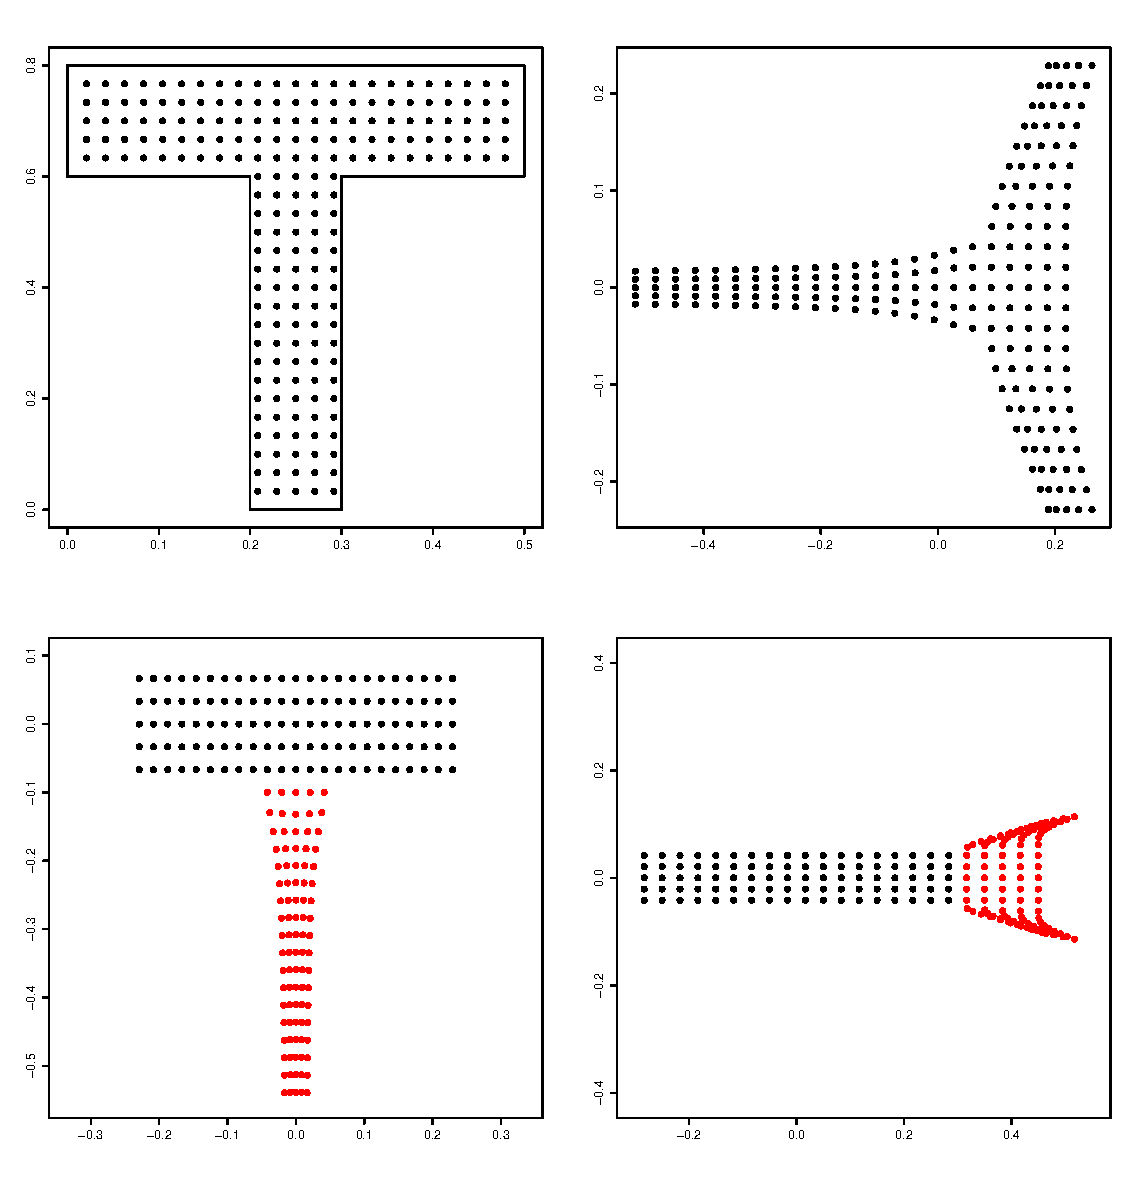
\includegraphics[width=3.5in]{mds/figs/tshape.pdf} \\
\caption{Data generated inside a T-shape (top left) is fed into MDS at once (top right). When either the head or tail of the T is used for the original MDS configuration and the other points inserted, the shape produced is distorted.}
\label{tshape}
% generated using figs/gridtest.R
\end{figure}

Although the cases show in \fig{tshape} are somewhat pathological, looking at more reasonable situations still leads to wildly different results. In \fig{tshaperand} the black and green points make up the original MDS configuration; the five green points are chosen at random. The red points are then inserted. As can be seen in these four typical realisations, the shape of the MDS space is dependent on those points used to create the initial MDS configuration.

% showing the the grid is necessary using the T shape (random samples
\begin{figure}
\centering
% trim order l b r t
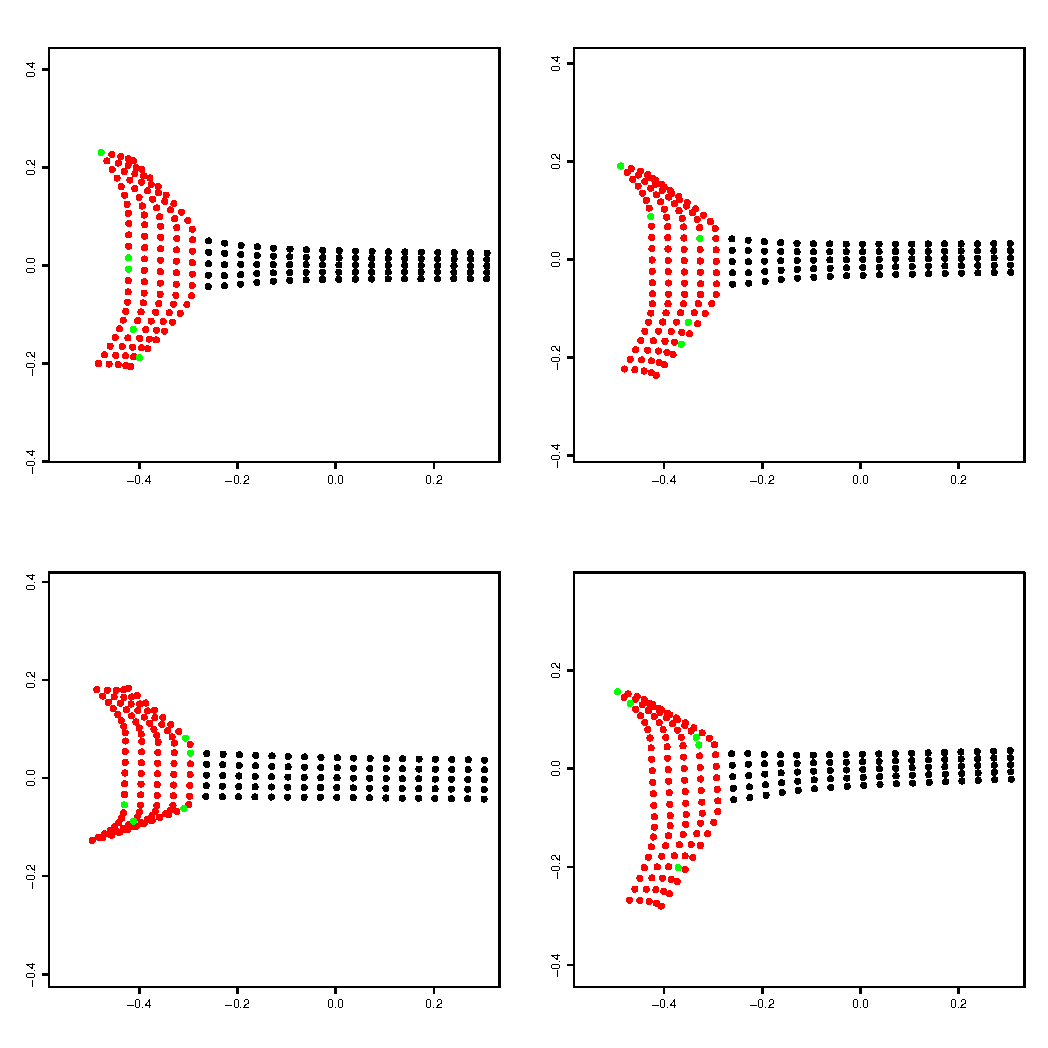
\includegraphics[width=3.5in]{mds/figs/tshaperand.pdf} \\
\caption{Using the T-shape in \fig{tshape} (top left), the tail (black points) of the T was used with 5 randomly sampled (green) points in the head. The head (without the 5 green points) was then inserted into the MDS configuration (red). As can be seen from these four realisations, the output varies greatly depending on the points sampled.}
\label{tshaperand}
% generated using figs/gridtest.R
\end{figure}

Hence, although there are the usual problems with predicting outside of the data, the added problem of the instability of MDS insertion can only confound results further. (Again, this is mentioned at the end of Gower's paper).

This problem can be rectified by using an appropriately spaced grid on the domain to calculate the eigen-decomposition, thus ensuring that the whole domain is covered. The base MDS configuration is then stable, provided that the grid is fine enough to catch all of the important features in the boundary of the domain.

\subsubsection{Smoothness of mapping}
\label{mds-smoothness}

Following from this, it is important to make sure that the MDS space is smooth in the sense that a grid of smooth lines over the domain are mapped to a series of smooth lines without discontinuities or sudden changes in direction. Taking the evenly spaced 50 by 50 point grid in \fig{wt2-grid-orig}, first MDS is performed on a dense point set of size 1253, and then a less dense grid is inserted using the method of Gower. The grid produced under the insertion can be seen in \fig{wt2-grid-full}. Taking a sample of 250 points from the 1253, an MDS configuration was also found and the same grid inserted (see \fig{wt2-grid-samp}). From this it is clear that those points mapped into the domain are smooth but in the sample case the features in the far right of the shape (the less pronounced peninsulae) are slightly squashed.

% grid to map
\begin{figure}
\centering
% trim order l b r t
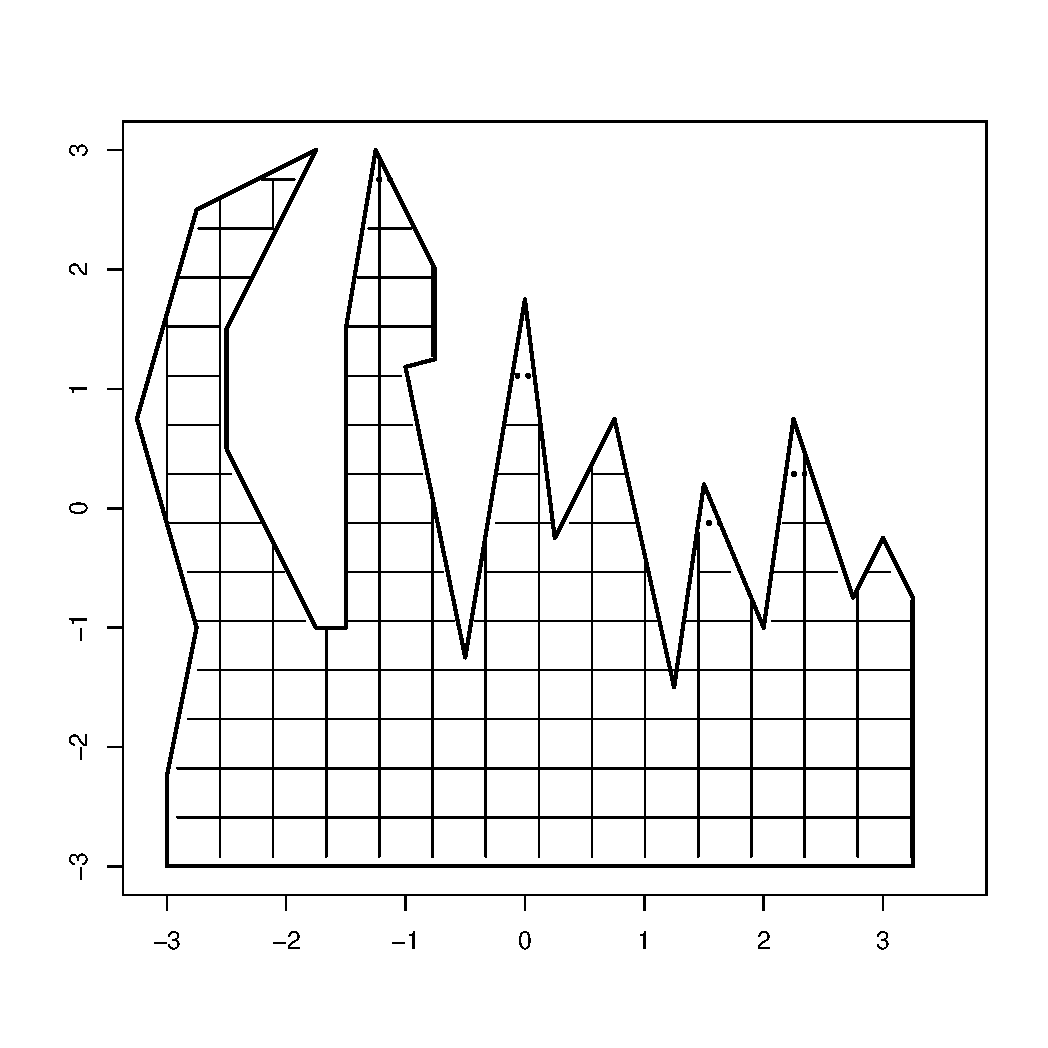
\includegraphics[width=4in]{mds/figs/wt2-grid-orig.pdf} \\
\caption{The grid to be inserted into the MDS configuration over the peninsula domain to test the smoothness of the mapping.}
\label{wt2-grid-orig}
% generated using wt2-grid.R
\end{figure}

% mapped grid (full)
\begin{figure}
\centering
% trim order l b r t
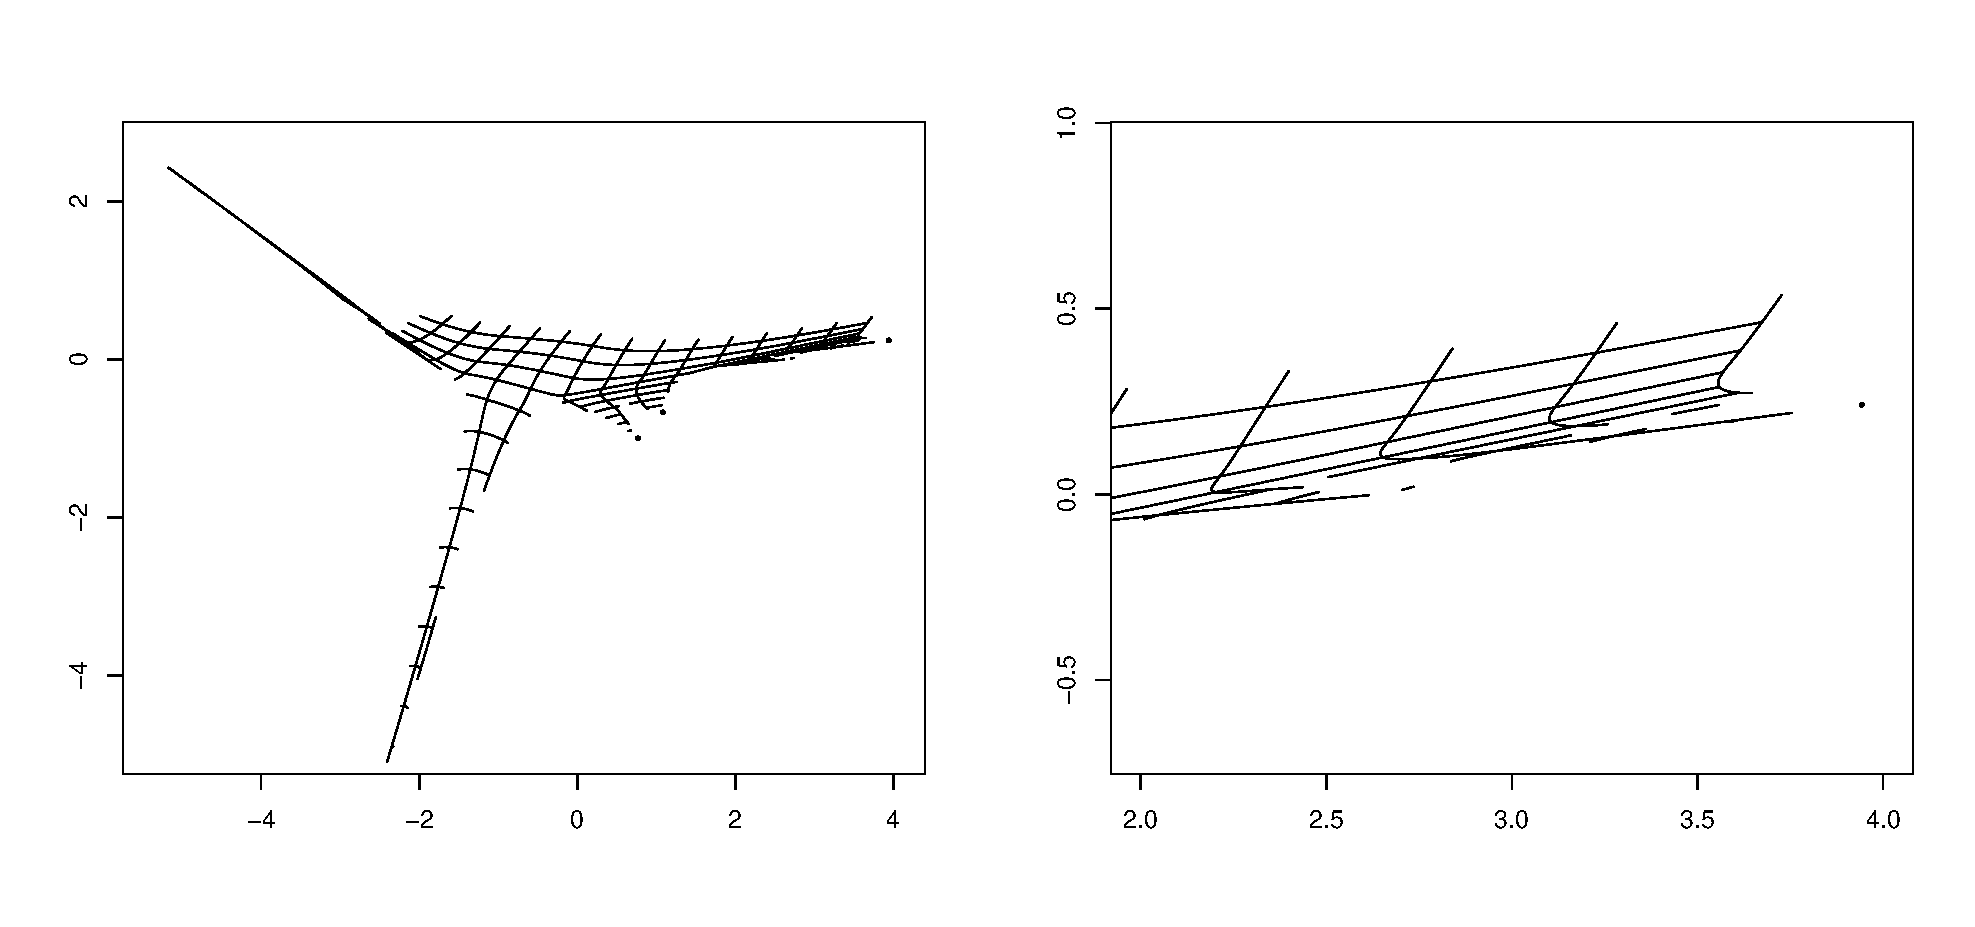
\includegraphics[width=5in]{mds/figs/wt2-grid-full.pdf} \\
\caption{Inserted grid when 1253 points are used to create the initial MDS configuration. The right panel shows a zoom of the far right part of the configuration.}
\label{wt2-grid-full}
% generated using wt2-grid.R
\end{figure}

% mapped grid (samp)
\begin{figure}
\centering
% trim order l b r t
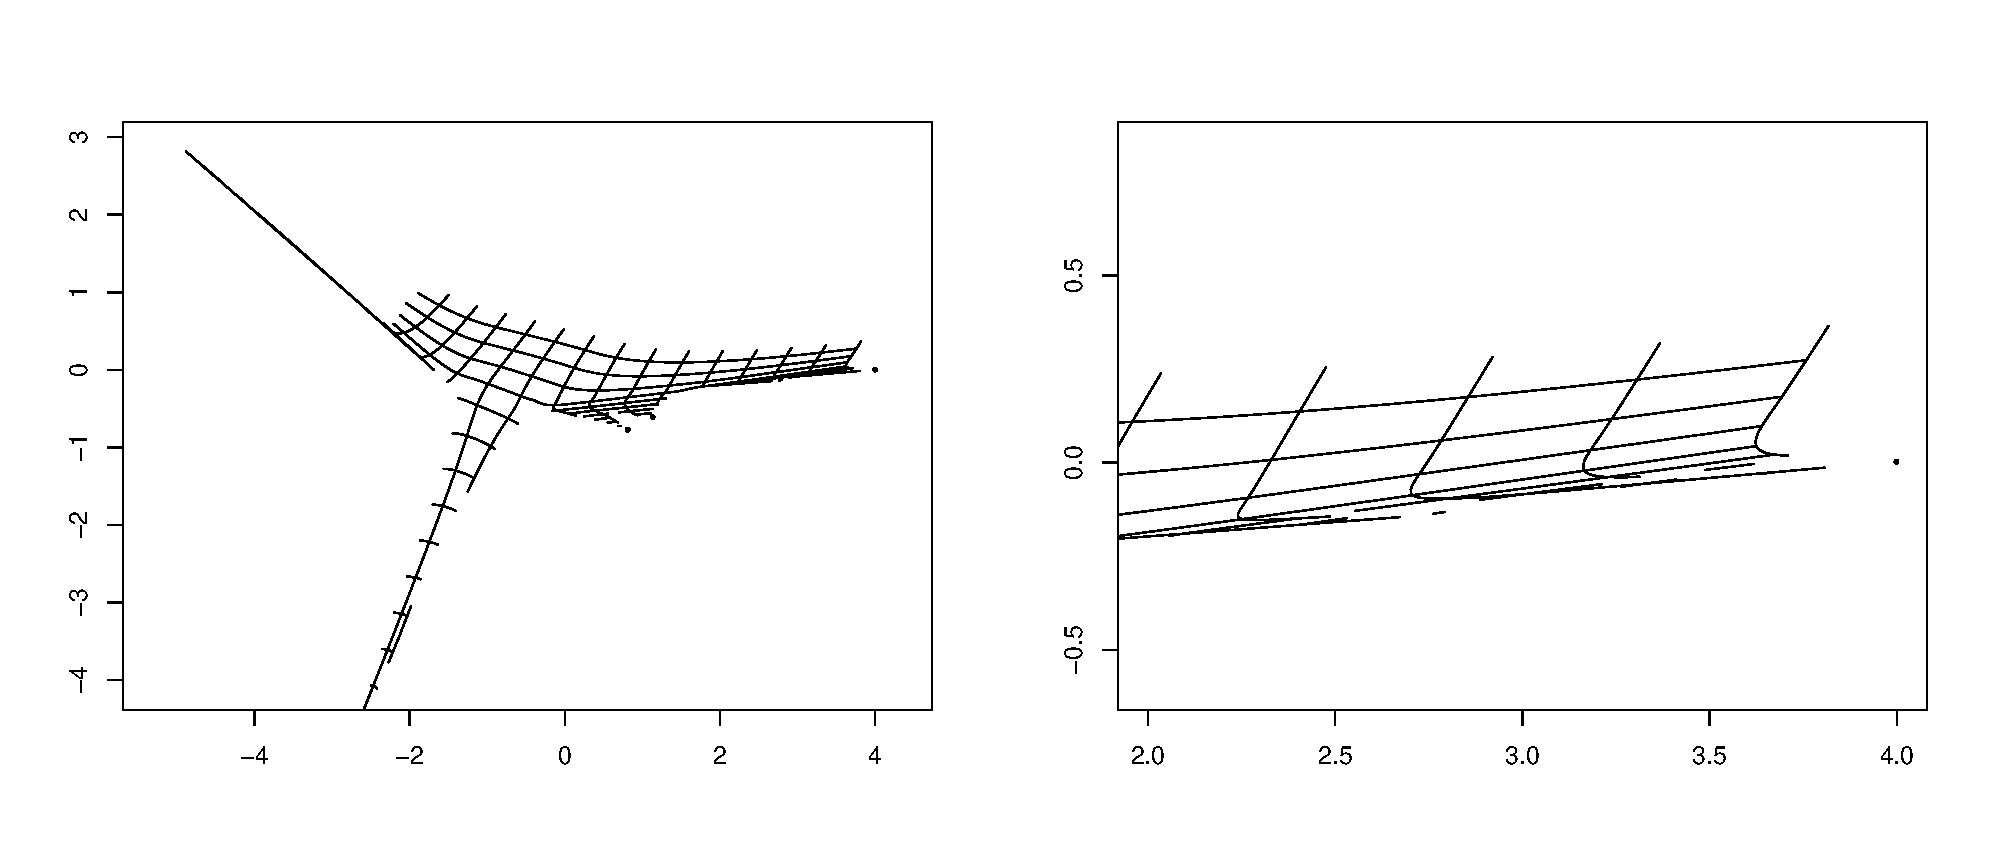
\includegraphics[width=5in]{mds/figs/wt2-grid-samp.pdf} \\
\caption{Inserted grid when 250 randomly chosen points are used to create the initial MDS configuration. The right panel shows a zoom of the far right part of the configuration. Comparing this to that of \fig{wt2-grid-full}, one can see that the features on the right have been squashed together.}
\label{wt2-grid-samp}
% generated using wt2-grid.R
\end{figure}

In conclusion, the mapping can be both reliable and also produces a smooth configuration of points provided that the initial MDS configuration covers the space in sufficient detail.


\section{Finding the within-area distances}
\label{mdsdist}
In order to perform multidimensional scaling the matrix of distances must be found. This section describes a novel algorithm to find the within-area distances.

Let the domain boundary be some polygon, $\Gamma$. Given that there is no direct path within the domain between two points ($p_1$ and $p_2$, say), the algorithm proceeds as follows to create a path (ie. an ordered set of edges and vertices), $\mathcal{P}$:

\begin{enumerate}
\item (INIT) Start by drawing a line between $p_1$ and $p_2$ (\fig{wdia}, ($i$)). Start the path as the lines from $p_1$, $p_2$ to their nearest intersection with the boundary of $\Gamma$ ($p_1^1$, $p_2^1$, say). Then form two paths. The first path from $p_1^1$ to $p_2^1$ ($\mathcal{P}_1$) contains the vertices of $\Gamma$ found moving along the boundary from $p_1^1$ to $p_2^1$. The second ($\mathcal{P}_2$), is found by taking the path from $p_1^1$ to $p_2^1$ in the other direction around the boundary, ie. the vertices of $\Gamma$ not in the first path. It is easy to see that $\{\mathcal{P}_1 \cup \mathcal{P}_2\} \setminus \{p_1^1, p_2^1\} = \Gamma$. The DELETE step (below) is then performed on $\mathcal{P}_1$ and $\mathcal{P}_2$, removing any superfluous vertices. Finding the length of $\mathcal{P}_1$ and $\mathcal{P}_2$ and choosing the shorter ($\mathcal{P^*}$), the initial path is formed as $\mathcal{P}=(p_1,p_1^1,\mathcal{P}^*,p_2^1,p_2)$. 

In \fig{wdia}, ($iii$), $\mathcal{P}_1$ is marked in green and is chosen to form the initial path, $\mathcal{P}=(p_1,p_1^1,\mathcal{P}_1,p_2^1,p_2)$, as $\mathcal{P}_1$ is shorter than $\mathcal{P}_2$, in red.

\item (DELETE) Given a triple of vertices, $(v_i, v_{i+1}, v_{i+2}) \in \mathcal{P}$ , if the line between $v_i$ and $v_{i+2}$ is shorter than the path $(v_i, v_{i+1}, v_{i+2})$ and the line between $v_i$ and $v_{i+2}$ lies inside $\Gamma$ then delete $v_{i+1}$ (\fig{wdia}, ($iv$) and ($vi$)). The entire path is iterated over deleting all superfluous vertices until there are no changes in successive runs. 

For example in \fig{wdia} ($iii$), $v_2$ is deleted from $\mathcal{P}$ because the path straight between $v_1$ and $v_3$ is shorter, and within $\Gamma$.

\item (ALTER) Given a triple of vertices $(v_i, v_{i+1}, v_{i+2}) \in \mathcal{P}$, if the path $\mathcal{P}_{ID}$ is shorter than the path $(v_i, v_{i+1}, v_{i+2})$ then replace $(v_i, v_{i+1}, v_{i+2})$ with $\mathcal{P}_{ID}$ (\fig{wdia}, ($v$)). The candidate replacement path, $\mathcal{P}_{ID}$, is calculated by running INIT with $p_1$ and $p_2$ replaced by $v_i$ and $v_{i+2}$, producing $\mathcal{P}_I$, and then using DELETE on $\mathcal{P}_I$ to remove superfluous vertices, giving $\mathcal{P}_{ID}$.

For example in \fig{wdia} ($iv$), the path $(v_1, v_2, v_3)$ is longer than the path $\mathcal{P}_{ID}=(v_1, v^1_2, v_3)$ (green dashed line in ($iv$)) so the former is replaced with the latter in $\mathcal{P}$. The path created by INIT is marked as $\mathcal{P}_{I}$ in  ($iv$) in red.

\item (ITER) We then iterate further DELETE and ALTER steps until there has been no change in $\mathcal{P}$ from one run to the next (ie. convergence) (\fig{wdia}, ($vi$)).
\end{enumerate}

% diagram for finding the shortest path in W
\begin{sidewaysfigure}
\centering
% trim order l b r t
\psfrag{exp1}[]{$\mathcal{P}_1$}
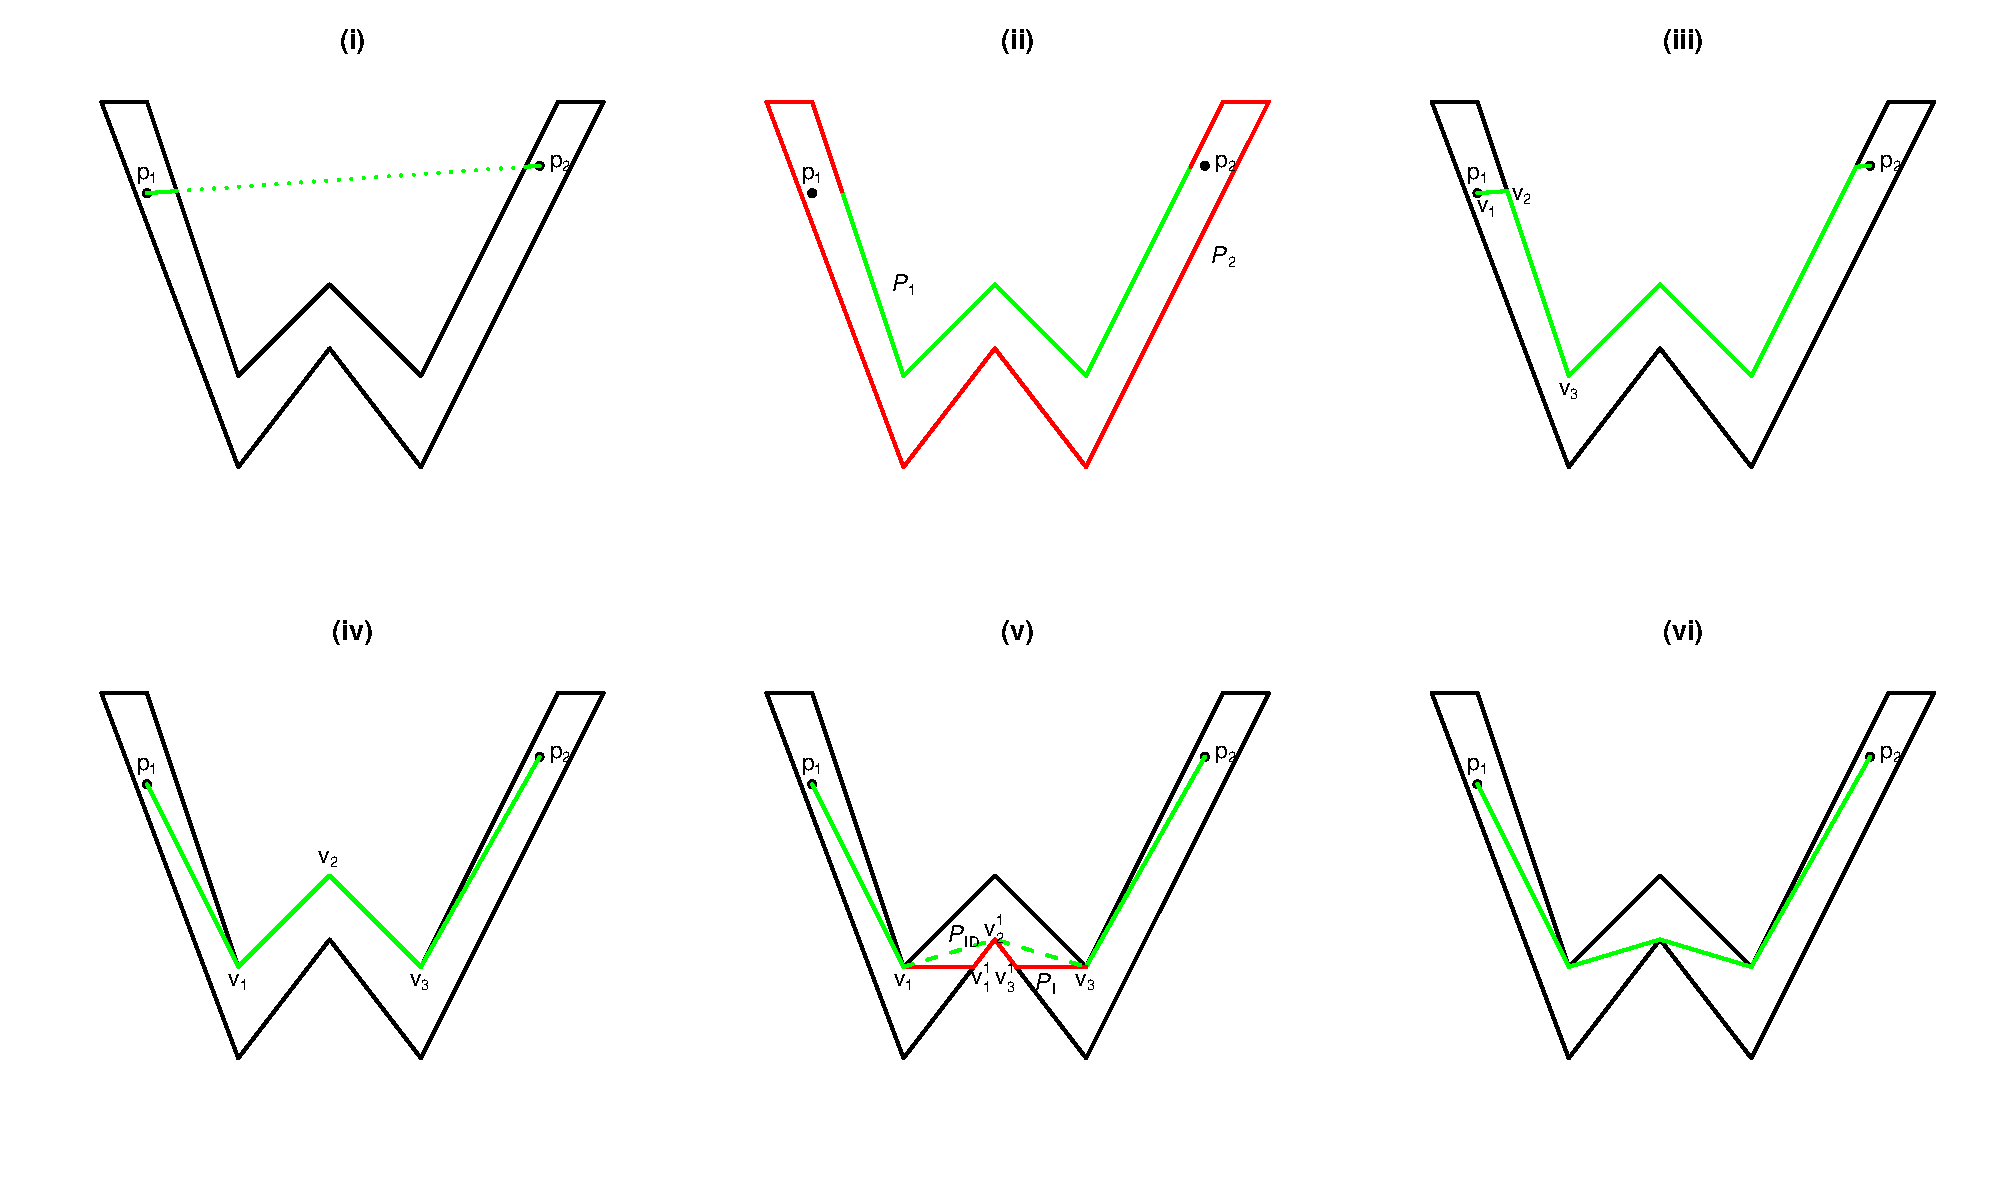
\includegraphics[trim=0in 0.5in 0in 0.25in, width=9.5in]{mds/figs/wdia.pdf} \\
\caption{The green lines in ($i$) to ($vi$) show the steps forming the shortest path as the algorithm progresses from initial state to final, shortest path (bottom right). See \secref{mdsdist}.}
\label{wdia}
% generate /phd-smoothing/mds-writeup/figs/distanceexplanation.R
\end{sidewaysfigure}

Of course, if there is a direct path between $p_1$ and $p_2$ then the Euclidean distance between the points can be used.

\section{Simulation experiments}
\label{mdssims}

In order to investigate the efficacy of \mdsap, a series of simulation experiments were performed. In all cases the results for \mdsap\ were compared to those of the current best method (the soap film smoother) and the standard approach of a {\tprs\} was used (which will not account for leakage).

The \textsf{R} packages \texttt{mgcv} and \texttt{soap} with additional bespoke software for finding the within-area distances were used. In all cases smoothing parameter estimation was performed using GCV (see \secref{GAMGCV}).

\subsection{The Ramsay horseshoe}

Again, we start with the modified Ramsay horseshoe since it clearly illustrates the problem of leakage; if a general method is to be useful it must first perform well on even a simple case such as this.

\subsubsection{Setup}

For the horseshoe, samples of 250 points with normal errors (at 3 levels:  $\sigma= $ 0.1, 1 and 10) were taken. (These are the settings used in \cite{soap}.) Using these samples, three models were fitted to the data. Predictions were then made over 718 points (including the sample locations). 200 realisations were generated and the EDF and MSE recorded for each replicate. The three models fitted were as follows:

\begin{enumerate}
\item \emph{Thin plate spline}: bivariate \tprs\  with basis size 100.
\item \emph{Soap film smoother}: 32 knots evenly spread over a grid over the domain, cyclic spline on the boundary was of basis size 39.
\item \emph{\mdsap}: Used a thin plate spline of basis dimension 100. The initial MDS grid was 20 points wide by 10 points tall.
\end{enumerate} 

Note that due to time and computational restrictions, the boundary was reduced from the 160 vertex polygon in the \texttt{fs.boundary()} function in \texttt{soap} to a 21 vertex polygon by only using every 8$^\text{th}$ vertex. This should not cause a major difference in results even if the soap film used the full boundary and \mdsap\ used only the reduced set of edges, since objective is to allow the smoother to get a broad idea of the topology of the domain, rather than the minutiae of the boundary features.

\subsubsection{Results}

Predictions from a typical realisation can be seen from \fig{mds-ramsay-fit-1}, where $\sigma=1$ with a sample size of 250. Both the soap film smoother and \mdsap\ are able to reproduce the main features of the true horseshoe function due to their ability to respect the boundary (in the case of the soap film) or the geometry of the domain (in the case of \mdsap). The \tprs\ shows leakage as expected. This is reflected in table \ref{ramsayresultstable} where we see that the soap film smoother and \mdsap\ have significantly smaller average MSE. When the noise level is high the \mdsap\ outperforms the soap film smoother in MSE terms (and is less variable).

\begin{table}[ht]
\centering
\begin{tabular}{c c c c}
 & & MSE & \\ 
$\sigma$ & \mdsap & Soap film & Thin plate\\ 
\hline
0.1  & 0.0032 (3$\cross10^{-5}$) & 0.0022 (3$\cross10^{-5}$) & 0.0402 (0.0008) \\ 
1  & 0.0436 (0.0015) & 0.0482 (0.0014) & 0.2306 (0.0024) \\ 
10  & 2.0652 (0.1215) & 3.0702 (0.2382) & 3.3713 (0.1133) \\ 
\end{tabular}
\begin{tabular}{c  c c c }
&  & EDF & \\ 
$\sigma$ & \mdsap & Soap film & Thin plate\\ 
\hline
0.1 & 47.613 (0.3497) & 39.164 (0.26) & 92.5996 (0.1020)\\ 
1  & 8.3828 (0.3452) & 11.868 (0.4010) & 46.607 (0.4238)\\ 
10 & 5.0577 (0.3324) & 5.5863 (0.2876) & 5.9786 (0.2511)\\ 
\end{tabular}
\caption{Mean MSE and estimated degrees of freedom (EDF) for the three models fitted to the modified Ramsay horseshoe function with standard errors (in brackets) over 200 realisations. Sample size was 250 with error levels given in the column marked $\sigma$.}
\label{ramsayresultstable}
\end{table}

The EDFs in table \ref{ramsayresultstable} show that \mdsap\ fits a less complex model than the thin plate spline on average, and for the two higher error situations, has a lower EDF than the soap film. Given that this is coupled with a lower MSE, it appears that \mdsap\ simultaneously yields both a more accurate and less complex model than the soap film for the horseshoe when there is a high level of noise. When noise is lower, the soap film and \mdsap\ MSEs are still of the same order. \Fig{mds-ramsay-boxplot} shows the logarithm of the per-realisation average MSE for each of the models at each error level.

% boxplot for Ramsay
\begin{figure}
\centering
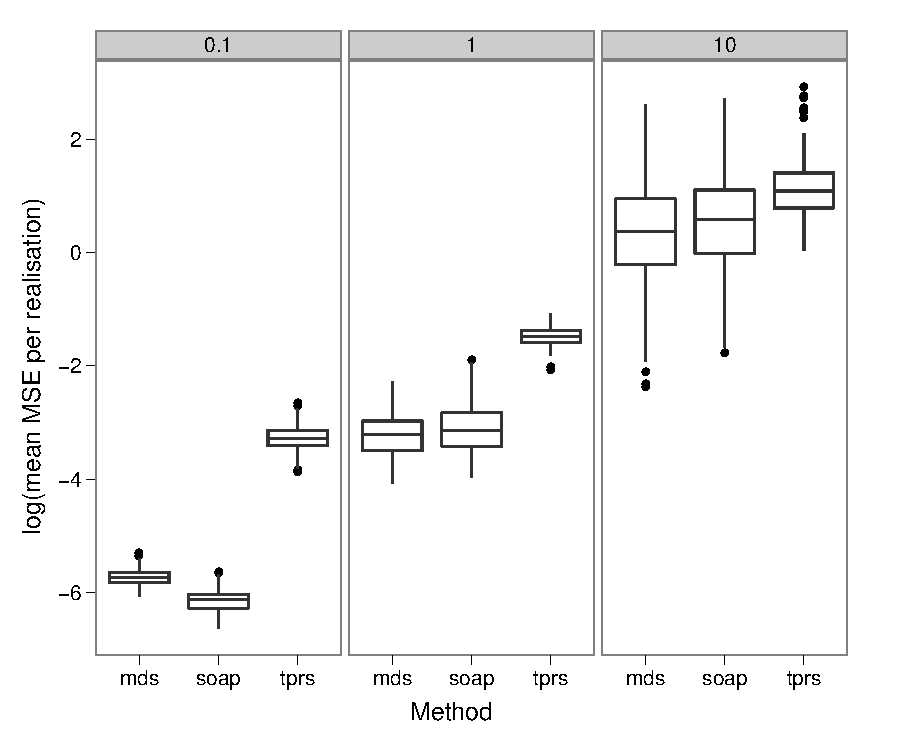
\includegraphics[width=6in, trim=0in 0.5in 0in 0in]{mds/figs/mds-ramsay-boxplot.pdf} \\
\caption{Boxplots of the logarithm of the MSE per realisation of the Ramsay horseshoe for \mdsap\, the soap film smoother and \tprs\ for error levels $\sigma=$ 0.1, 1 and 10 (left to right, respectively). In all cases, a Wilcoxon signed rank test showed that MSEs for \mdsap\ and \tprs\ were significantly different from the soap film smoother ($\text{p-value} < 10^{-2}$).}
\label{mds-ramsay-boxplot}
% generated using phd-smoothing/mds/sim/ramsay-boxplots.R
% Wilcoxon test in phd-smoothing/mds/sim/ramsay-wilcox.R
\end{figure}

% Ramsay fit with error=1 
\begin{figure}
\centering
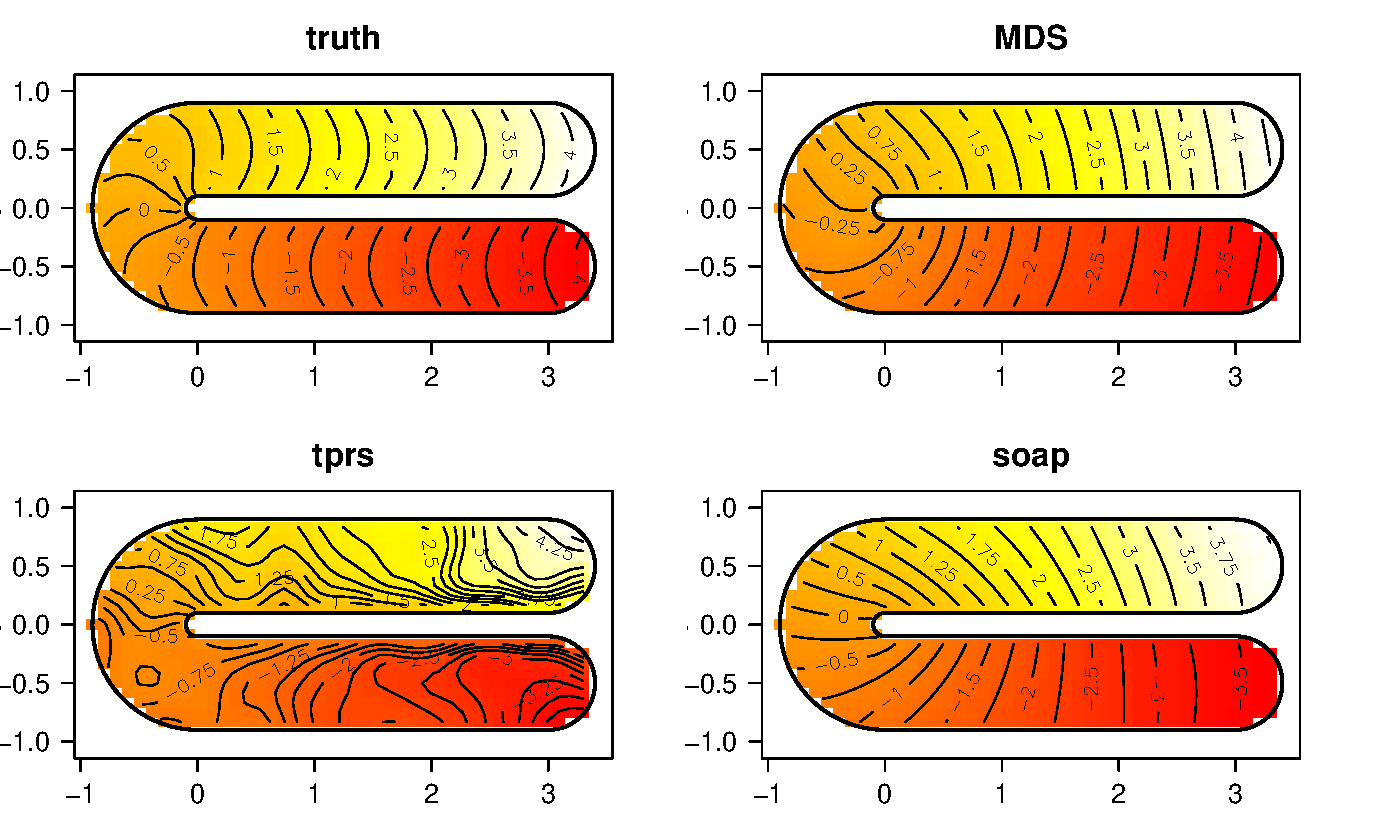
\includegraphics[width=6in]{mds/figs/ramsay-fit-1.pdf} \\
\caption{Top left: truth for the (modified) Ramsay horseshoe. Others: a typical realisation of fits from the three models when 250 points are sampled with noise set to $\sigma=1$.}
\label{mds-ramsay-fit-1}
% generated (roughly) using ramsay-smooth-test.R
\end{figure}

Just as when the \sch\ transform was used to morph the domain, it is interesting to see what has happened to the distribution of points in space. \Fig{mdsrampoints} shows the effect of the transform on a regular grid of points (left) when they are projected into MDS space (right). The projection has also succeeded in parting the two arms of the horseshoe, reducing leakage (as can be seen in the realisations in \fig{mds-ramsay-fit-1}).

\begin{figure}
\centering
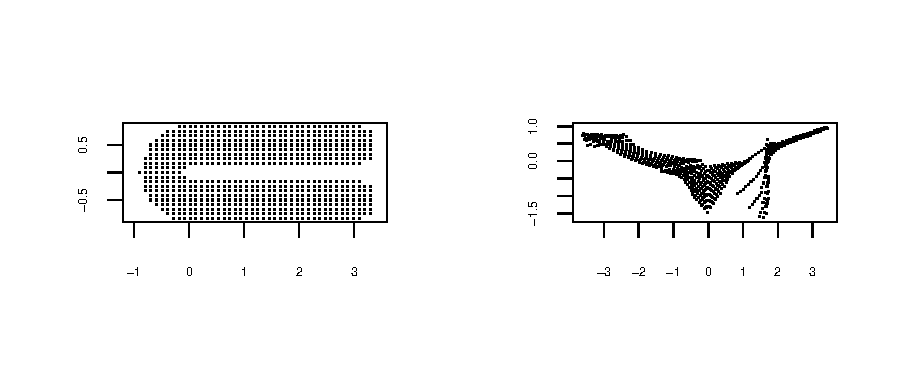
\includegraphics[width=6in,trim=0.5in 0.5in 0in 0.5in]{mds/figs/mdsrampoints.pdf} \\
\caption{A regular grid over the Ramsay horseshoe (left) and its projection into MDS space (right).}
\label{mdsrampoints}
% generated using thesis/mds/figs/mdsrampoints
\end{figure}


\subsection{Peninsula domain}
\label{mds-wt2-sim}

The Ramsay horseshoe is an easy domain to smooth over since it is clear that a transformation should be parting the two arms of the domain. In practise however, there may be ambiguity over which parts of the domain should be separated the most. For this reason a more realistic, complex domain would provide a better insight into the efficacy of the method. The domain shown in \fig{wt2-truth} is an approximation to a coastline with a strong trend along both peninsulae (in a manner similar to that of the horseshoe) but with the added complication of a further peak in the lower right corner.

\subsubsection{Setup}

The simulations consisted of 200 realisations of 250 samples from the surface in \fig{wt2-truth}. Normal errors were added at three levels $\sigma=$ 0.35, 0.9, and 1.55 (corresponding to signal-to-noise ratios (SNRs) of 0.95, 0.75 and 0.5, respectively. SNRs were calculated as the mean squared correlation between true function value and the truth with error added). Mean squared error over 1253 prediction points (including those points in the sample) was calculated and recorded, along with EDF for each model. The models fitted were:

% wt2 truth 
\begin{figure}
\centering
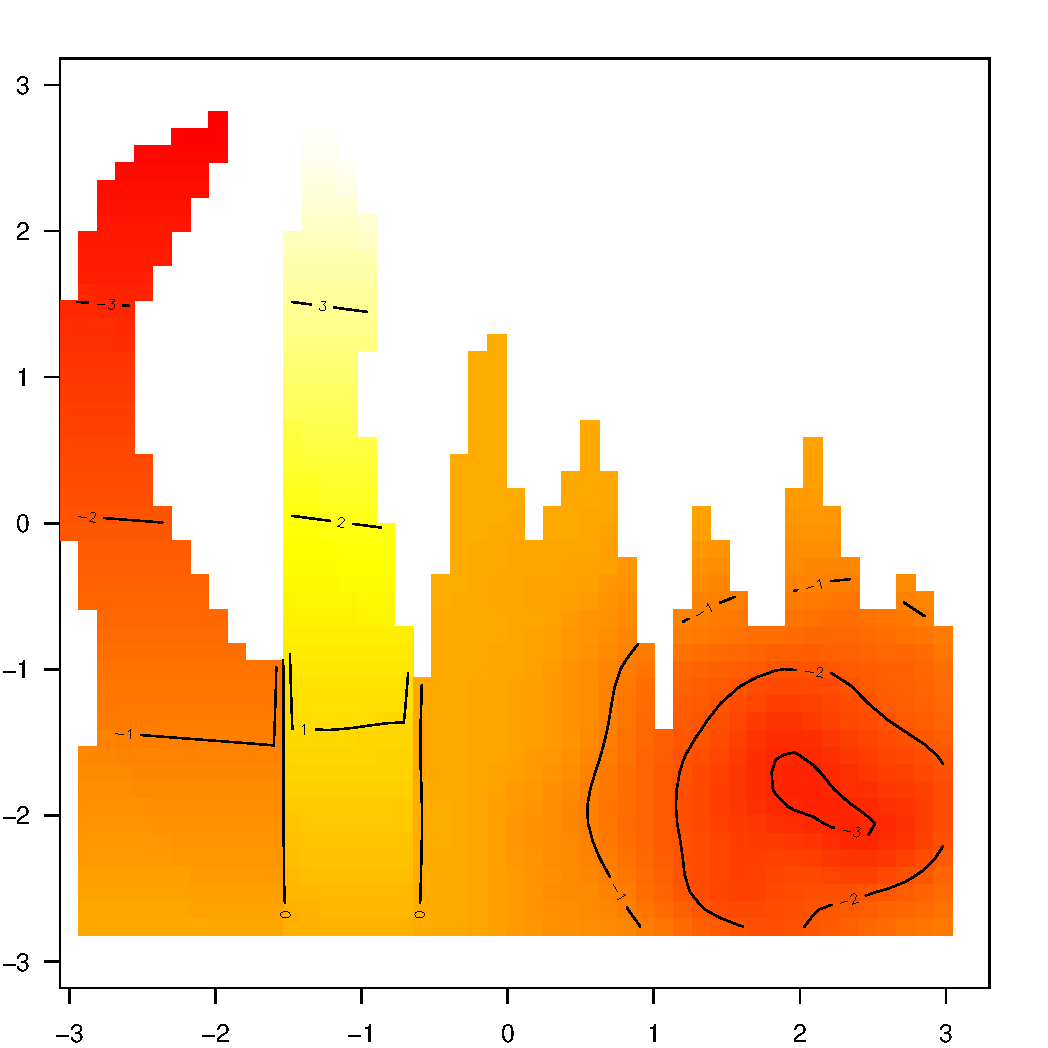
\includegraphics[width=3in]{mds/figs/wt2-truth.pdf} \\
\caption{True function for the domain with multiple peninsulae.}
\label{wt2-truth}
% generated (roughly) using wt2-smooth-test.R
\end{figure}

\begin{enumerate}
\item \emph{Thin plate spline}: bivariate thin plate spline with basis size 100. 
\item \emph{Soap film smoother}: cyclic spline on boundary of basis size 60, 109 internal knots evenly spaced on a grid over the domain.
\item \emph{\mdsap}: after transform a bivariate thin plate spline with basis size 100 was fit. The initial MDS grid was 10 by 10 points square (48 points were inside).
%\item \emph{MDS with tensor product}: tensor product of two thin plate splines, each of basis dimension 12. The initial MDS grid was 74 points square.
\end{enumerate} 

\subsubsection{Results}

% wt2 fit with error=0.9
\begin{figure}
\centering
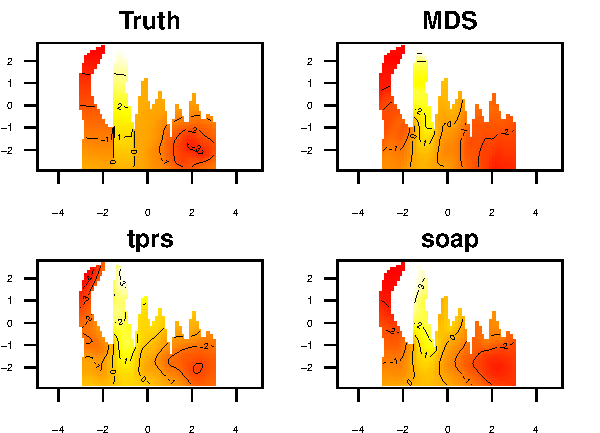
\includegraphics[width=6in]{mds/figs/wt2-comp-09.pdf} \\
\caption{A typical realisation of fits from the multiple peninsulae domain when $\sigma$ is set to 0.9 (SNR = 0.75) and sample size is 250. Prediction grid was of size 1253. Clockwise from top left: the true function, prediction from: MDS projection smoothed with \tprs, the soap film smoother and \tprs.}
\label{wt2-comp-0.9}
% generated (roughly) using wt2-smooth-test.R
\end{figure}

Looking at a typical realisation in \fig{wt2-comp-0.9} ($\sigma=$ 0.9, SNR = 0.75, sample size 250), the \tprs\ can be seen showing signs on leakage across the two main peninsulae, whereas \mdsap\ and the soap film do not show this. However the \tprs\ does reproduce the peak in the lower right much more faithfully, the other two smoothing over it. In this realisation, \mdsap\ deals with the values inside the peninsula a little better than the soap film smoother (the contour lines are closer to those in the true function). On the other hand, the soap film captures the shape of the lower right peak slightly more accurately.

Table \ref{wt2resultstable} gives the MSE and EDF for the models above averaged over 200 realisations. There is not a massive difference between the results in MSE terms, the soap film smoother consistently has a lower MSE, although not by much. The soap film also tends to fit simpler models than the other two approaches. The boxplots of the logarithm of the per-realisation MSEs are shown in \fig{mds-wt2-boxplot}.

% boxplot for wt2
\begin{figure}
\centering
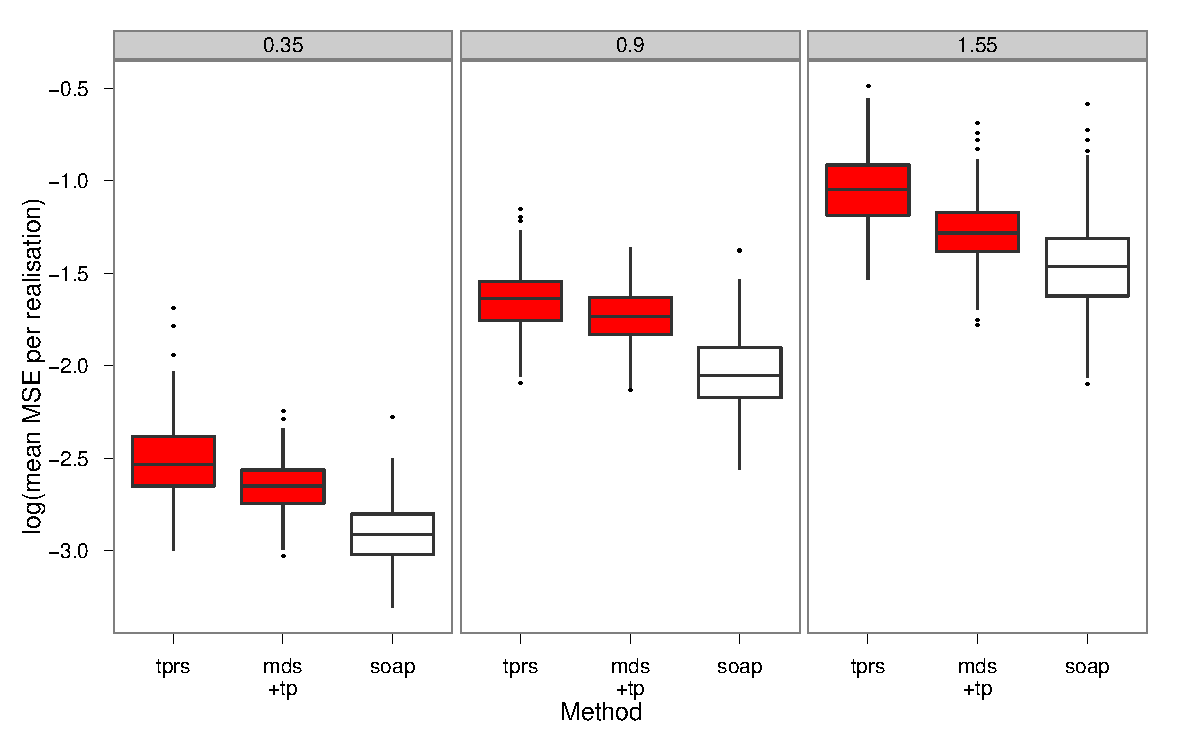
\includegraphics[width=6in, trim=0in 0.5in 0in 0in]{mds/figs/mds-wt2-boxplot.pdf} \\
\caption{Boxplots of the logarithm of the MSE per realisation of the peninsula domain for the MDS approach, soap film smoother and \tprs\ for error levels $\sigma=$ 0.35, 0.9 and 1.55 (left to right, respectively). A Wilcoxon signed rank test shows that the MSEs for \tprs\ were significantly different from those of the soap film smoother ($\text{p-value} < 10^{-2}$) at all noise levels. For \mdsap\ the two lower noise cases were significantly different from the soap film smoother, but not when $\sigma=1.55$ ($\text{p-value} = 0.023951$).}
\label{mds-wt2-boxplot}
% generated using phd-smoothing/mds/sim/wt2-boxplots.R
\end{figure}

\begin{table}[ht]
\centering
\begin{tabular}{c c c c c}
 &  & MSE  & &\\ 
$\sigma$ & \mdsap & Soap film & Thin plate\\ 
\hline
0.35  & 0.07 (0.00062) & 0.0539 (5e-04) &0.082 (0.00104)\\
0.9  & 0.177 (0.00184) & 0.1308 (0.00197) &0.1938 (0.00241)\\
1.55  & 0.2859 (0.00438) & 0.2362 (0.00434) &0.3509 (0.00471)\\
\end{tabular}
\begin{tabular}{c c c c c}
 &  & EDF  & &\\ 
$\sigma$ & \mdsap & Soap film & Thin plate\\ 
\hline
0.35 &80.9039 (0.57103) & 55.6979 (0.51448) & 77.9619 (0.46726)\\ 
0.9 &35.0185 (0.76449) & 29.7171 (0.57477) & 48.0508 (0.47636)\\ 
1.55 &19.4625 (0.57265) & 20.2918 (0.36634) & 32.2715 (0.47961)\\ 
\end{tabular}
\caption{Mean MSE and EDF for the four models fitted to the peninsula domain with standard errors (in brackets) over 200 realisations.}
\label{wt2resultstable}
\end{table}

As with the Ramsay horseshoe, it is interesting to see what the projection into MDS space has done to the distribution of the points in the domain. \Fig{wt2-2d-proj} shows points in the domain in Euclidean space and MDS space. There appears to be some high concentrations of points in the far left peninsula and in the right side in the MDS space. This is due to the projection from $n$-dimensional space into 2-dimensional space, which can be easily seen in \fig{wt2-3d-proj} where the points have been projected into 3-dimensional space. This shows that there is separation between the smaller peninsulae in higher dimensions that cannot be seen in the 2-dimensional projection.

This high point density in the right side of the MDS space could be the reason for the poor reproduction of the function in that region, seen in \fig{wt2-comp-0.9}. In this portion of space (and in the left peninsula) there is a breakdown in isotropy, which the \tprs\ does not handle well. This must be accounted for in the smooth if accurate models are to be built.

% how the points are projected for wt2
\begin{figure}
\centering
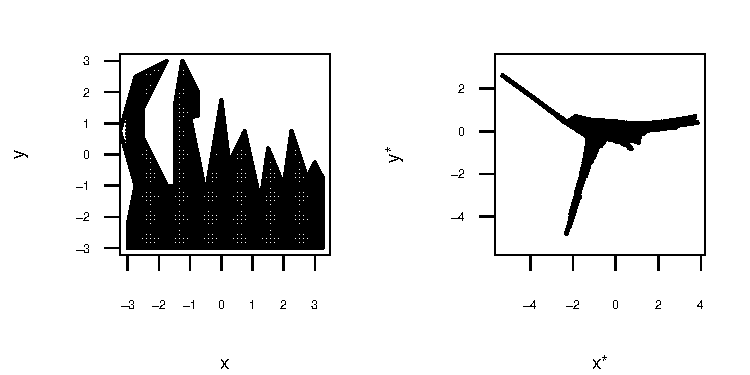
\includegraphics[width=6in]{mds/figs/wt2-2d-proj.pdf} \\
\caption{A regular grid over the peninulae domain (left) and its projection into MDS space (right).}
\label{wt2-2d-proj}
% generated using thesis/mds/figs/wt2-mds.R
\end{figure}

% how the points are projected for wt2 in 3D!
\begin{sidewaysfigure}
\centering
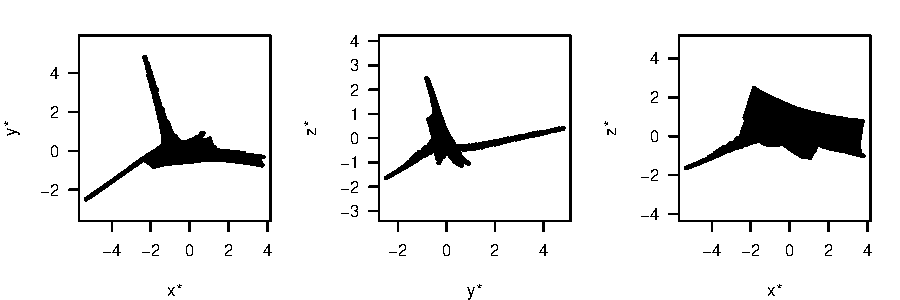
\includegraphics[width=9in]{mds/figs/wt2-3d-proj.pdf} \\
\caption{The peninsula domain projected into 3-dimensional MDS space. The plots show combinations of axes, note that the $x^*,y^*$ combination is the same as the 2-dimensional projection in \fig{wt2-2d-proj}.}
\label{wt2-3d-proj}
% generated using thesis/mds/figs/wt2-mds.R
\end{sidewaysfigure}

\subsection{Areas for improvement}

From this set of simulations areas for improvement to \mdsap\ can be seen. First, the above problem of the accuracy of the model (in terms of faithfully reproducing the function) needs to be addressed. Second, running the model is actually quite slow, the calculation of the within-area distances by the algorithm given in \secref{mdsdist} has considerable computational cost, even in comparison to the soap film smoother basis setup. Table \ref{wt2time} shows the average timings for running \mdsap, \tprs\ and soap film smoothers over the peninsula domain

\begin{table}[ht]
\centering
\begin{tabular}{c || c c c c c c}
 & \mdsap & Soap film & Thin plate\\ 
\hline
Fit & 84.85242 & 24.6783 & 0.4022\\ 
Prediction &  53.5105 & 29.3946 & 0.1249\\
\end{tabular}
\label{wt2time}
\caption{Average time (in seconds) to fit and predict on a realisation of the peninsula domain for the four models considered above. Times are averaged over 100 realisations and were found using the elapsed time provided by \textsf{R}'s built-in \texttt{system.time} function. For each realisation a sample of size 250 was taken, then a 1253 values were predicted.}
\end{table}

In order to make \mdsap\ worthwhile for a practitioner to use the method, it would be preferable for it not only to have a sensible physical model, but also outperform the soap film smoother in either (or both) of accuracy and speed.

\section{Improvements}
\label{MDSimprov}

This section focuses on strategies to improve the above method in terms of speed and accuracy. The first part looks at the speed of \mdsap, the latter on the accuracy. 

\subsection{Making \mdsap\ faster}
\label{mds-faster}

\subsubsection{Calculating MDS by Lanczos iteration}

The \textsf{R} command used to perform the multidimensional scaling, \texttt{cmdscale}, uses the routine \texttt{eigen} in order to perform the requisite matrix eigen-decomposition. This routine will calculate a full eigen-decomposition of the matrix, even if only the first $k$ eigenvalues and/or eigenvectors are required. Using Lanczos iteration, only the first $k$ eigenvalues (in numeric or algebraic size order) will be calculated.

The  Lanczos procedure works by iteratively building a symmetric $i\cross i$ tridiagonal matrix (at the $i^{\text{th}}$ iteration) which has eigenvalues approximately the same as the $i$ largest eigenvalues of the original matrix. Further detail is given in \cite{simonbook}, pp. 335-337.

The \texttt{igraph} library for \textsf{R} provides an interface to the C++ package \texttt{ARPACK++} which implements the Lanczos procedure. Replacing the \texttt{cmdscale} command with one that uses the \texttt{ARPACK++} interface provided by \texttt{igraph} will decrease the number of computations needed, thus making the calculation of the eigenvalues and vectors faster.

A quick benchmark shows that \texttt{ARPACK++} can compute the first two eigenvalues and vectors faster than just using \texttt{eigen} when the eigen-decomposition to be computed is of a large matrix. Generating a 1000 by 1000 symmetric matrix of Normal random variates with mean 0 and variance 1000, then performing an eigen-decomposition takes 1.68 seconds using \texttt{ARPACK++} and 3.26 seconds using \texttt{eigen} (averaged over 100 runs). This advantage drops once the matrix is around 100 by 100 and the cost of calling the C++ code begins to dominate; in this case \texttt{ARPACK++} takes 0.037 seconds and \texttt{eigen} takes 0.034 (over 100 runs). Given that the disadvantage is in the order of hundredths of a second and the advantage is a two-fold decrease in computational time, it makes sense to use the \texttt{ARPACK++} code in all cases.

% sim code is at ~/phd-smoothing/mds/lanczos/time-arpack.R

\subsubsection{Partial path calculation}

Many of the distances stored in $D$ are calculated by simply using the Euclidean metric since for the corresponding point pairs, there is no part of the path between them that lies outside of the domain. It is often the case that the paths that need to be calculated are on a grid (for example, when doing prediction). This leads us to believe that there are many sets of paths that are rather similar. These paths may perhaps only differ in their final vertex. Given that, in this case, there is a lot of wasted computational time spent calculating similar paths, it would be useful to exploit this problem, and use it to increase the speed of the path calculation.

The idea here is to use a sparse grid to first calculate a set of paths that are then saved. These saved paths are then form the base of the other paths that need to be calculated. Finally, these paths are optimised in the same manner as the algorithm given in \secref{mdsdist}. This removes the expensive calculation in the middle of the path, where perhaps the bulk of the interactions with the boundary take place.

The algorithm is as follows, with notation and routines (INIT, DELETE, ALTER and ITER) identical to those in \secref{mdsdist}. 

Again, taking points $p_i$ and $p_j$ in the set of points in the domain that we wish to find the shortest paths for and drawing a path between them, finding within-area distance with respect to the boundary of $\Gamma$.

\begin{enumerate}
 \item Begin by creating a sparse grid of within $\Gamma$ and calculate the ($M$, say) non-Euclidean within-area paths between all pairs of points exactly as in \secref{mdsdist}. Store these paths as $\mathcal{P}_1,\ldots, \mathcal{P}_M$.
\item For each unique pairing of $p_i$ and $p_j$ in the full data set, calculate the path using one of the following:
	\begin{enumerate}
	\item Find a $\mathcal{P}_k$ such that the path between $p_i$ and one end of $\mathcal{P}_k$ and $p_j$ and the other end of $\mathcal{P}_k$ is Euclidean within $\Gamma$. Join $p_i$ and $p_j$ onto the appropriate ends of $\mathcal{P}_k$ and run ITER (ie. alternate between DELETE and ALTER) until convergence.
	\item If there is no Euclidean path between $p_i$ and $p_j$, and no $\mathcal{P}_k$ can be found, then calculate the path between $p_i$ and $p_j$ as in \secref{mdsdist}. 
	\end{enumerate}
\end{enumerate}

Note that those paths between points in the sparse grid which are Euclidean are not stored since it is always at least as expensive to store, add and optimise those paths then calculating them from scratch. An argument towards why is this is true is as follows: if the path we want to calculate is Euclidean anyway, then retrieving a Euclidean path, adding in $p_i$ and $p_j$, and then iterating over ALTER and DELETE steps to make it both the shortest and a Euclidean path will take longer than just creating a Euclidean path to begin with. If the path between $p_i$ and $p_j$ is non-Euclidean then the non-Euclidean part of the path must lie outside $\mathcal{P}_k$ (by definition) and therefore will take the same number of operations to find the boundary crossing points and calculate the shortest path around the feature locally as it will to calculating the whole path from scratch.


\subsubsection{Simulation - Lanczos and partial path calculation improvements}

Taking both the Lanczos procedure and the partial path calculation together, a simulation was run to find the improvements in terms of computational time for the double peninsulae domain. Average time for both model fitting and prediction are given in \tabref{wt2itime} for 100 realisations. 

The differences between the first two columns are striking. The partial path calculation has dramatically reduced the computational time for the calculation of the entries of the distance matrix, making it faster than the soap film smoother for the model fitting, and reducing the prediction time to a third of its previous value. The \tprs\ times are shown to give a comparison for the time actually taken to fit the model, the remaining time for \mdsap\ is taken up by calculating the distances and performing the MDS.

\begin{table}[ht]
\centering
\begin{tabular}{c || c c c c c c}
%  no speedup           speedup
 & \mdsap & \mdsap (\textit{pp}) & Soap film & Thin plate\\ 
\hline
Fit & 84.85242 & 18.6526 & 24.6783 & 0.4022\\ 
Prediction & 155.4004 & 53.5105 & 29.3946 & 0.1249\\
\end{tabular}
\label{wt2itime}
\caption{Average time (in seconds) to fit and predict on a realisation of the peninsula domain for the four models considered above. Times are averaged over 100 realisations and were found using the elapsed time provided by \textsf{R}'s built-in \texttt{system.time} function. For each realisation a sample of size 250 was taken, then a 1253 values were predicted. For the \mdsap\ columns \textit{pp} indicates the cases where the partial paths were pre-calculated, those not marked use the algorithm given in \secref{mdsdist}.}
\end{table}


\subsection{Improving the accuracy of \mdsap\ by adjusting the penalty}
\label{mds-penadjust}

The higher MSEs shown in \tabref{wt2resultstable} at lower noise levels might be explained by the change in density of points in the domain after it has been transformed into MDS space and the way in this changes the measure of smoothness. In this case it makes sense to adjust the penalty in order to take into account the change in point density in MDS space.

\cite{wood2000} shows that given some transform of a variable, $y$ say, such that $y_i^\prime=y_i/k$, then $f(x,y^\prime k)$ will give the same fit as $f(x,y)$ (ie. the fit will be the same under the new coordinates). In this case the penalty will change to:
\begin{equation}
\int\int_\Omega \Big( \frac{\partial^2 f}{\partial x^2} \Big)^2 + 2k\Big( \frac{\partial^2 f}{\partial x \partial y} \Big)^2 + k^3\Big( \frac{\partial^2 f}{\partial y^2} \Big)^2 \text{d}x \text{d}y,
\label{adjustedintegral}
\end{equation}
from the usual \tprs\ penalty (see \secref{GAMtprspenalty}).

This approach will only handle a linear rescaling in one dimension; in the case of the MDS distortions, non-linear re-scalings in two dimensions must be addressed. To generalise \eqn{adjustedintegral} to the non-linear two-dimensional case a function must be found, $\mathcal{L}^*(x,y)$ say, which evaluates to the change in density for each point in the domain. 

Such a function should allow the smoothness to be adapted according to the degree to which space has been squashed, thus getting around the spatial heterogeneity which appears to be affecting the model. The calculation of $\mathcal{L}^*(x,y)$ is elaborated on below.

Given that the function $\mathcal{L}^*(x,y)$ is known, the penalty is given as:
\begin{equation}
\int\int_\Omega \mathcal{L}^*(x,y) \Big( \Big(\frac{\partial^2 f(x,y)}{\partial x^2}\Big)^2 + 2\Big(\frac{\partial^2 f(x,y)}{\partial x \partial y}\Big)^2 + \Big(\frac{\partial^2 f(x,y)}{\partial y^2}\Big)^2\Big) \text{d}x\text{d}y.
\label{kdeadjust}
\end{equation}
Note the change of integration domain from $\mathbb{R}^2$ to $\Omega$ (the transformed domain), as well as the pre-multiplication by the density function.

\subsection{Penalty adjustments in one dimension}

Before implementing this approach in full a a test was run in one dimension. The function:
\be
g(x)=0.2x^{11}(10(1-x))^6+10(10x)^3(1-x)^{10},
\label{hardfcn}
\ee
was used and contracted by factors of $20,1,0.05,1$ over the regions $[0,0.4], (0.4,0.6],(0.6,0.8],(0.8,1]$, respectively. The function and its squashed form are shown in the top left and right panels (respectively) of \fig{1dadjust}. Evaluating 100, equally spaced, points over the interval $[0,1]$ using a \tprs\ and then predicting back onto the same points yielded the blue lines in the lower two plots. The left of these shows the prediction in the transformed space and the right in the original space. The green line was produced using a \tprs\ with the adjusted penalty matrix. As can be seen from the plot, the fit has been improved greatly. We now look at the calculation of the adjustment to the penalty.

% 1d adjustment 2x2 diagram
\begin{figure}
\centering
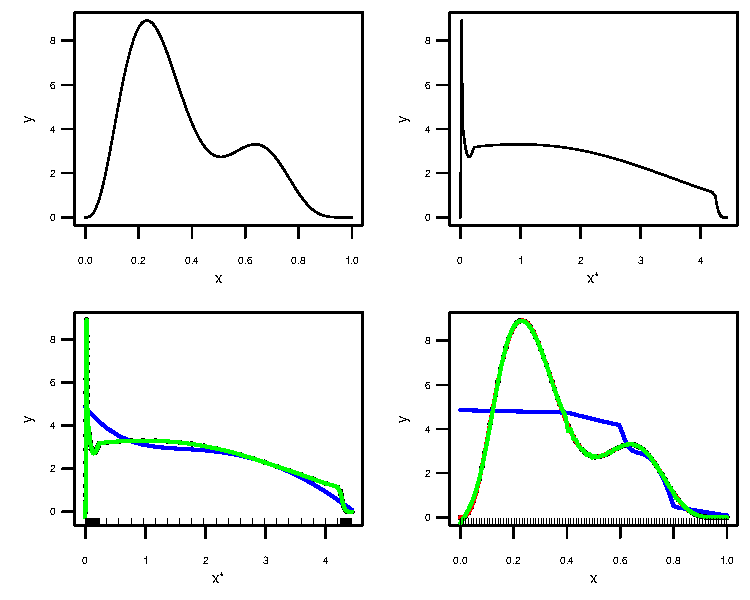
\includegraphics[width=6in]{mds/figs/1dadjust.pdf} \\
\caption{Using penalty adjustments to fit a regression spline to \eqn{hardfcn} after it has been squashed. The function in the top left is squashed to the form in the top right. The bottom left plot shows the fit from a \tprs\ (blue) and a \tprs\ with adjusted penalty (green) in the transformed space. The bottom right shows the same fit in the untransformed space. Clearly, the penalty adjustment improves the fit.}
\label{1dadjust}
% generated by thesis/mds/figs/tpintexp.R
\end{figure}

\subsubsection{Penalty adjustment calculation}

For the moment let us take $\hat{f}$ to be a one dimensional smooth function. It may be decomposed into its basis functions and coefficients in the usual way:
\be
\hat{f}(x)=\sum_{j=1}^J \hat{\beta}_j b_j(x) = \tr{\hat{\bm\beta}}\bm{b}(x).
\ee
The $ij^\text{th}$ element of the penalty matrix (see \secref{GAMpenalties}) is given as:
\be
S_{ij}= \int_a^b \mathcal{L}^*(x) \frac{\partial^2 b_i(x)}{\partial x^2}\frac{\partial^2 b_j(x)}{\partial x^2} \text{d}x = \int_a^b \mathcal{L}^*(x) b^{\prime\prime}_i(x) b^{\prime\prime}_j(x) \text{d}x,
\ee
in one dimension (letting a prime indicate differentiation with respect to $x$). The integral can then be approximated by the midpoint rule as:
\be
S_{ij}= \frac{b-a}{K}\sum_{k=1}^K \mathcal{L}^*(x_k) b^{\prime\prime}_i(x_k) b^{\prime\prime}_j(x_k) \quad \text{for} \quad x_k=a+\frac{(k-0.5)(b-a)}{K},
\label{midpointS}
\ee
for $k=1,\dots, K$. Second derivatives are evaluated by finite differences in the usual manner:
\be
\label{bfinitediff}
b^{\prime\prime}_i(x) = \frac{ b_i(x+2\epsilon) - 2b_i(x+\epsilon) + b_i(x)}{\epsilon^2}.
\ee
For the sake of efficiency, we in fact calculate a $K\cross J$ matrix $D$ with $kj^\text{th}$ element:
\be
D_{kj}=\sqrt{\mathcal{L}^*(x_k)} b^{\prime\prime}_j(x_k),
\label{oneDD}
\ee
for $x_k$ as above. Then $S$ may be calculated as:
\be
S=\frac{b-a}{K}\tr{D}D.
\ee

In this example $\mathcal{L}^*(x)$ was simply calculated using the inverse of the cube of the factor by which the relevant part of the domain (given above) was squashed. 

\subsubsection{Checking that the adjustment works}

\Fig{1dadjust} shows that the adjustment faithfully repdroduces $g(x)$ for the zero error case, fitting a much more sensible model than the standard \tprs. To check that this is true more generally, $\lambda$ was specified (rather than being automatically selected) so that the models with modified and unmodified penalties would have the same EDF. \Fig{1dedfdia} shows such an experiment. Using \eqn{hardfcn} with Normal(0, 0.4) noise added the smoothing parameter was set so that the EDF would be 71, 19 and 42 (working down the diagram). The plots show that the adjustment deviates from truth at most as badly as the vanilla \tprs\ but overall corrects some of the departures from the truth, even in presence of error with a restricted basis.

% 1d adjustment EDF comparison diagram
\begin{figure}
\centering
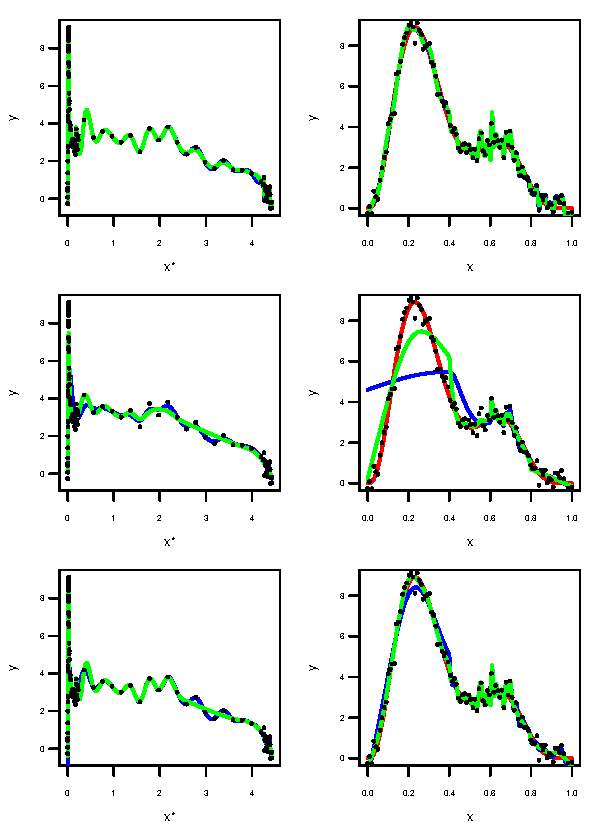
\includegraphics[width=5.5in]{mds/figs/1dedfdia.pdf} \\
\caption{Predictions in transformed and untransformed (left and right columns respectively) for \tprs\ (blue line) and penalty adjusted \tprs\ (green line) fits to the function in \eqn{hardfcn} when the smoothing parameter was pre set to give EDF of 71, 19, and 42 (top to bottom).}
\label{1dedfdia}
% generated by thesis/mds/figs/tpintexp.R
\end{figure}


\subsection{Penalty adjustments in two dimensions}

Using a similar procedures as for one dimension, the two dimensional case can be addressed. Again looking at the $ij^\text{th}$ element of $S$, for the two dimensional case we have:
\begin{equation}
S_{ij}=\int\int_\Omega \mathcal{L}^*(x,y) \Big( \frac{\partial^2 b_i(x,y)}{\partial x^2}\frac{\partial^2 b_j(x,y)}{\partial x^2}+2\frac{\partial^2 b_i(x,y)}{\partial x \partial y}\frac{\partial^2 b_j(x,y)}{\partial x \partial y}+\frac{\partial^2 b_i(x,y)}{\partial y^2}\frac{\partial^2 b_j(x,y)}{\partial y^2} \Big) \text{d}x\text{d}y.
\end{equation}
Matrices analogous to \eqn{oneDD} can be constructed using the finite differences from \eqn{bfinitediff} for differentials $x$ and $y$ individually and
\be
\frac{\partial^2 b_i(x,y)}{\partial x \partial y} = \frac{ b_i(x+\epsilon,y+\epsilon) - b_i(x+\epsilon,y) - b_i(x,y+\epsilon) + b_i(x,y)}{\epsilon^2},
\ee
for the cross term. The matrices then take the form:
\be
[D_x]_{kj}=\sqrt{\mathsf{K}(x_k,y_k)} \frac{\partial^2 b_j(x_k,y_k)}{\partial x^2},
\ee
\be
[D_y]_{kj}=\sqrt{\mathsf{K}(x_k,y_k)} \frac{\partial^2 b_j(x_k,y_k)}{\partial y^2},
\ee
\be
[D_{xy}]_{kj}=\sqrt{\mathsf{K}(x_k,y_k)} \frac{\partial^2 b_j(x_k,y_k)}{\partial x \partial y}.
\ee
So we may then express $S$ as:
\be
S=\tr{D_x}D_x + \tr{D_{xy}}D_{xy} + \tr{D_y}D_y.
\ee
Where the partial derivative evaluation points ($x_k$ and $y_k$) now form a grid for the integration to be calculated. First defining $x^\dagger_k$ and $y^\dagger_k$ analogously to \ref{midpointS}, we have:
\be
x^\dagger_k=a_x+\frac{(k-0.5)(b_x-a_x)}{K},\\
y^\dagger_k=a_y+\frac{(k-0.5)(b_y-a_y)}{K},
\ee
for $k=1,\dots,K$. The integration grid may then be constructed as:
\be
\{x_k : k=1,\dots,K\} = \{x^\dagger_1,x^\dagger_1,x^\dagger_1,\dots, x^\dagger_2, x^\dagger_2, x^\dagger_2,\dots, x^\dagger_K, x^\dagger_K, x^\dagger_K\},
\ee
\be
\{y_k : k=1,\dots,K\} = \{y^\dagger_1,y^\dagger_2, y^\dagger_3,\dots, y^\dagger_K,y^\dagger_1,y^\dagger_2, y^\dagger_3,\dots, y^\dagger_K,\dots\}.
\ee
Finally, those $(x_k,y_k)$ that do not lie inside the boundary in MDS space are removed leaving only those points that lie inside.

\subsubsection{Finding $\mathcal{L}^*$}

Calculating $\mathcal{L}^*(x,y)$ in two dimensions is more tricky than in the one dimensional case. Since the two-dimensional case is to be used in practise, the method for finding $\mathcal{L}^*(x,y)$ must depend on the MDS configuration, as the stretch factors will not be known \emph{a priori} (as was the case in the previous example).

The general idea is to make $\mathcal{L}^*(x,y)$ a function of the change in density of points caused by projecting the original space into MDS space. However, if we assume that the density in the untransformed space is $1$ everywhere, we merely need to calculate the density in MDS space. Having calculated the point density in MDS space, $\mathcal{L}^*(x,y)$ is just some function of this density.

In order to find calculate the point density in MDS space, the following steps are performed:

\begin{enumerate}
\item A grid in the original space is mapped into the MDS space. Ideally, this grid would be dense enough for it to be possible to just count the number transformed points in each square of a regular mesh. However, it would be computationally demanding to project a dense grid into MDS space, so instead a sparse grid is used and then interpolated. This consisted of taking 10 equally spaced points on each side of the square and drawing lines between points on opposing sides. Where the lines crossed were the extra points (along with those points lying on the boundary of the square itself).
\item The interpolated points are then used to estimate the overall point density in MDS space by simply counting the number of points there were in each of a set of squares made from the integration grid, call is $\mathcal{L}(x,y)$. This is shown in \fig{densgrid} for the double peninsulae domain. 
\item Then define $\mathcal{L}^*(x,y)$ as the function
\be
\mathcal{L}^*(x,y)=\frac{1}{(1+\mathcal{L}(x,y))^{3/2}}.
\ee
The $+1$ in the denominator ensures that we do not divide by zero when evaluating $\mathcal{L}^*(x,y)$. The fact that $\mathcal{L}^*(x,y)$ is then a piecewise function should not be too worrying since the aim here is to address the broader problems with the change in spatial density, not the fine-gained details.
\end{enumerate}

Note that the power is now $\frac{3}{2}$. This is since we do not know the contraction/expansion in each direction individually, but rather the overall change in area. As such we use $\frac{3}{2}$ rather than the cubic on $x$ and $y$ and unitary on the cross term.

\begin{figure}
\centering
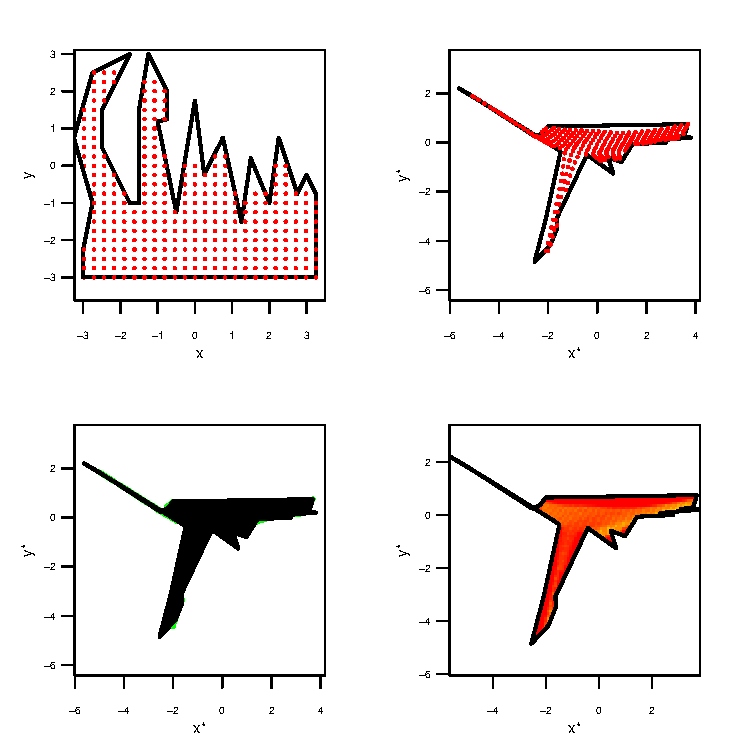
\includegraphics{mds/figs/densgrid.pdf} \\
\caption{The grids used to calculate $\mathcal{L}^*(x,y)$ for the double peninsulae domain. The red grid in the top left figure is mapped to the red grid in the top right panel. The red points in the top right are then used as the basis for the interpolation in the bottom left. The number of green points in each of the squares made from the black points in the bottom left plot are used to calculate the spatial density in that square. The heat map in the bottom right shows the values of $\mathcal{L}(x,y)$ (ie. the density of the green points), here red is low density, yellow is high. Note that some of the points lie outside of the boundary in the MDS projections. This is due to the boundary in MDS space being the straight line interpolant of the vertices of the boundary in the original space.}
\label{densgrid}
% generated by phd-smoothing/mds/wt2-intexp.R and intexp/smooth2.c.R with comments removed
\end{figure}

\subsubsection{Checking that the adjustment works}

In order to make sure that the adjustment works in both the known and unknown contraction/expansion case, a small simulation was run. In this case a surface consisting of two bivariate Normal distributions (mean vectors $(0,-0.5)$ and $(0,0.5)$, covariance matrix diagonal entries $(0.2,0.1)$) were sampled from (sample size 300) and then noise added from a $\text{Normal}(0,0.05)$ distribution. The surface was then divided into its four constituent quadrants about the origin and squashed according to the following factors (in $(x,y)$ pairs, in order top left, top right, bottom left, bottom right): ((0.3,5),(1,5),(0.3,1),(1,1)).

The samples were then used to fit a standard \tprs\ model, \tprs\ with adjusted penalty with known stretch factors and a \tprs\ with $\mathcal{L}^*(x,y)$ estimated from the data. The mean squared error between the truth and prediction over a dense (50 by 50) grid was then calculated.

The simulation results show that there is a decrease in MSE when the expansion/contraction of the space is taken into account (MSEs were: $2.355, 2.300 \text{and} 2.305$ for \tprs, known stretch and estimated stretch, respectively). Unfortunately this didn't offer the same visual improvement as the 1-dimensional case, so heat maps are not shown here.

The next section puts the adjusted penalty approach to the test on a number of domains and compares it to other possible models.

\section{Wider simulations and real data}

\subsection{Peninsulae domain}
\label{wt2bigsim}

Using the same setup as in \secref{mds-wt2-sim}, for each error level (0.35, 0.9 and 1.55), 200 realisations were generated. From these 250 samples were drawn to fit the model, predictions were over a grid of 1253 points with MSE and EDF recorded per model for each simulation. 

The models that were fitted were:
\begin{enumerate}
\item \emph{Thin plate spline}:  with basis size 140.
\item \emph{\mdsap}: using a \tprs\ with basis size 140.
\item \emph{\mdsap}: using a tensor product (see \secref{GAMtensor}) of cubic splines, each dimension of which had a basis size of 12.
\item \emph{\mdsap}: using a 3-dimensional \tprs\ with basis size 140. Here MDS was used to project the data into three dimensions rather than two.
\item \emph{\mdsap}: using a \tprs\ with basis size 140, with penalty adjustments.
\item \emph{Soap film smoother}: using 109 internal knots evenly spaced on a grid over the domain, with boundary basis size 60.
\end{enumerate}

As can be seen in \tabref{bigwt2resultstable}, the results from \mdsap\ with the adjustments are actually worse than those from just \mdsap. In all cases the \mdsap\ with adjusted penalty has a worse MSE than any of the other models; even the \tprs\ has a lower MSE in the two higher noise cases. \Fig{big-wt2-mses} shows box plots of these results.

However, all is not lost, the models using \mdsap\ with either 3-dimensional projection or the cubic regression spline are competitive across the board. In the case of the cubic regression spline, this is probably due to the tensor setup of the spline. Having a different smoothing parameter for each direction will allow the model to take care of the anisotropic space into which the data has been projected. In the high noise case the \tprs\ basis coupled with \mdsap\ has a lower and less variable MSE than the cubic regression spline, this may well be due to the \tprs\ enforcing the isotopy in a high-noise case and this constraint has lead to a less variable model being fitted, which happens to be closer to the truth in this case. As for the 3-D projection, the plots in \fig{wt2-3d-proj} show that the additional dimension allows for further separation of both a large and small peninsulae, which should help with the spatial heterogeneity as well as leakage.

A Wilcoxon signed rank test, matching pairs between realisations showed that there was a significant difference between the MSE each model and the soap film smoother. As can be seen from \fig{big-wt2-mses}, soap outperforms all of the other methods on this domain, with \mdsap\ (with 3-D projection) coming in second. 

Finally, note that there were three realisations omitted (for all models) in \tabref{bigwt2resultstable} and \fig{big-wt2-mses}. In these realisations the soap film smoother failed to fit the model due to knot placement. These can be safely removed as, in practise, the computer would inform the user that the knot placement was not appropriate and the knot layout could be altered.

\begin{sidewaystable}[p]
\centering
\begin{tabular}{c c c c c c c}
 & &  & MSE  & & &\\ 
$\sigma$  & tprs & mds+tp & mds+cr & mds+tp 3D & mds+tp+adj & soap\\ 
\hline
0.35  & 0.0832 (1e-04) & 0.0713 (5e-05) & 0.0633 (8e-05) & 0.058 (5e-05) & 0.0759 (6e-05) & 0.0598 (0.00032)\\ 
0.9  & 0.1957 (0.00017) & 0.1788 (0.00013) & 0.1652 (0.00025) & 0.1479 (0.00014) & 0.2413 (0.00022) & 0.1616 (0.00201)\\ 
1.55  & 0.3576 (0.00035) & 0.285 (0.00027) & 0.3198 (0.00063) & 0.2765 (0.00032) & 0.4778 (0.00048) & 0.245 (0.00034)\\ 
\end{tabular}
\begin{tabular}{c c c c c c c}
 & &  & EDF  & & &\\ 
$\sigma$  & tprs & mds+tp & mds+cr & mds+tp 3D & mds+tp+adj & soap\\ 
\hline
0.35  & 77.8675 (0.03803) & 80.5571 (0.04098) & 53.9331 (0.03577) & 61.3881 (0.05365) & 84.1456 (0.04092) & 55.2464 (0.04684)\\ 
0.9  & 47.0214 (0.0378) & 34.3451 (0.05633) & 31.9288 (0.03523) & 30.5663 (0.04034) & 50.6702 (0.04171) & 29.6874 (0.04514)\\ 
1.55  & 31.8803 (0.03843) & 18.3473 (0.03846) & 20.5101 (0.04256) & 19.7879 (0.03128) & 31.1969 (0.05291) & 20.3529 (0.03171)\\ 
\end{tabular}
\caption{Mean MSE and EDF for the six models fitted to the peninsula domain with standard errors (in brackets) over 200 realisations.}
\label{bigwt2resultstable}
\end{sidewaystable}

% big wt2 sim MSEs
\begin{sidewaysfigure}
\centering
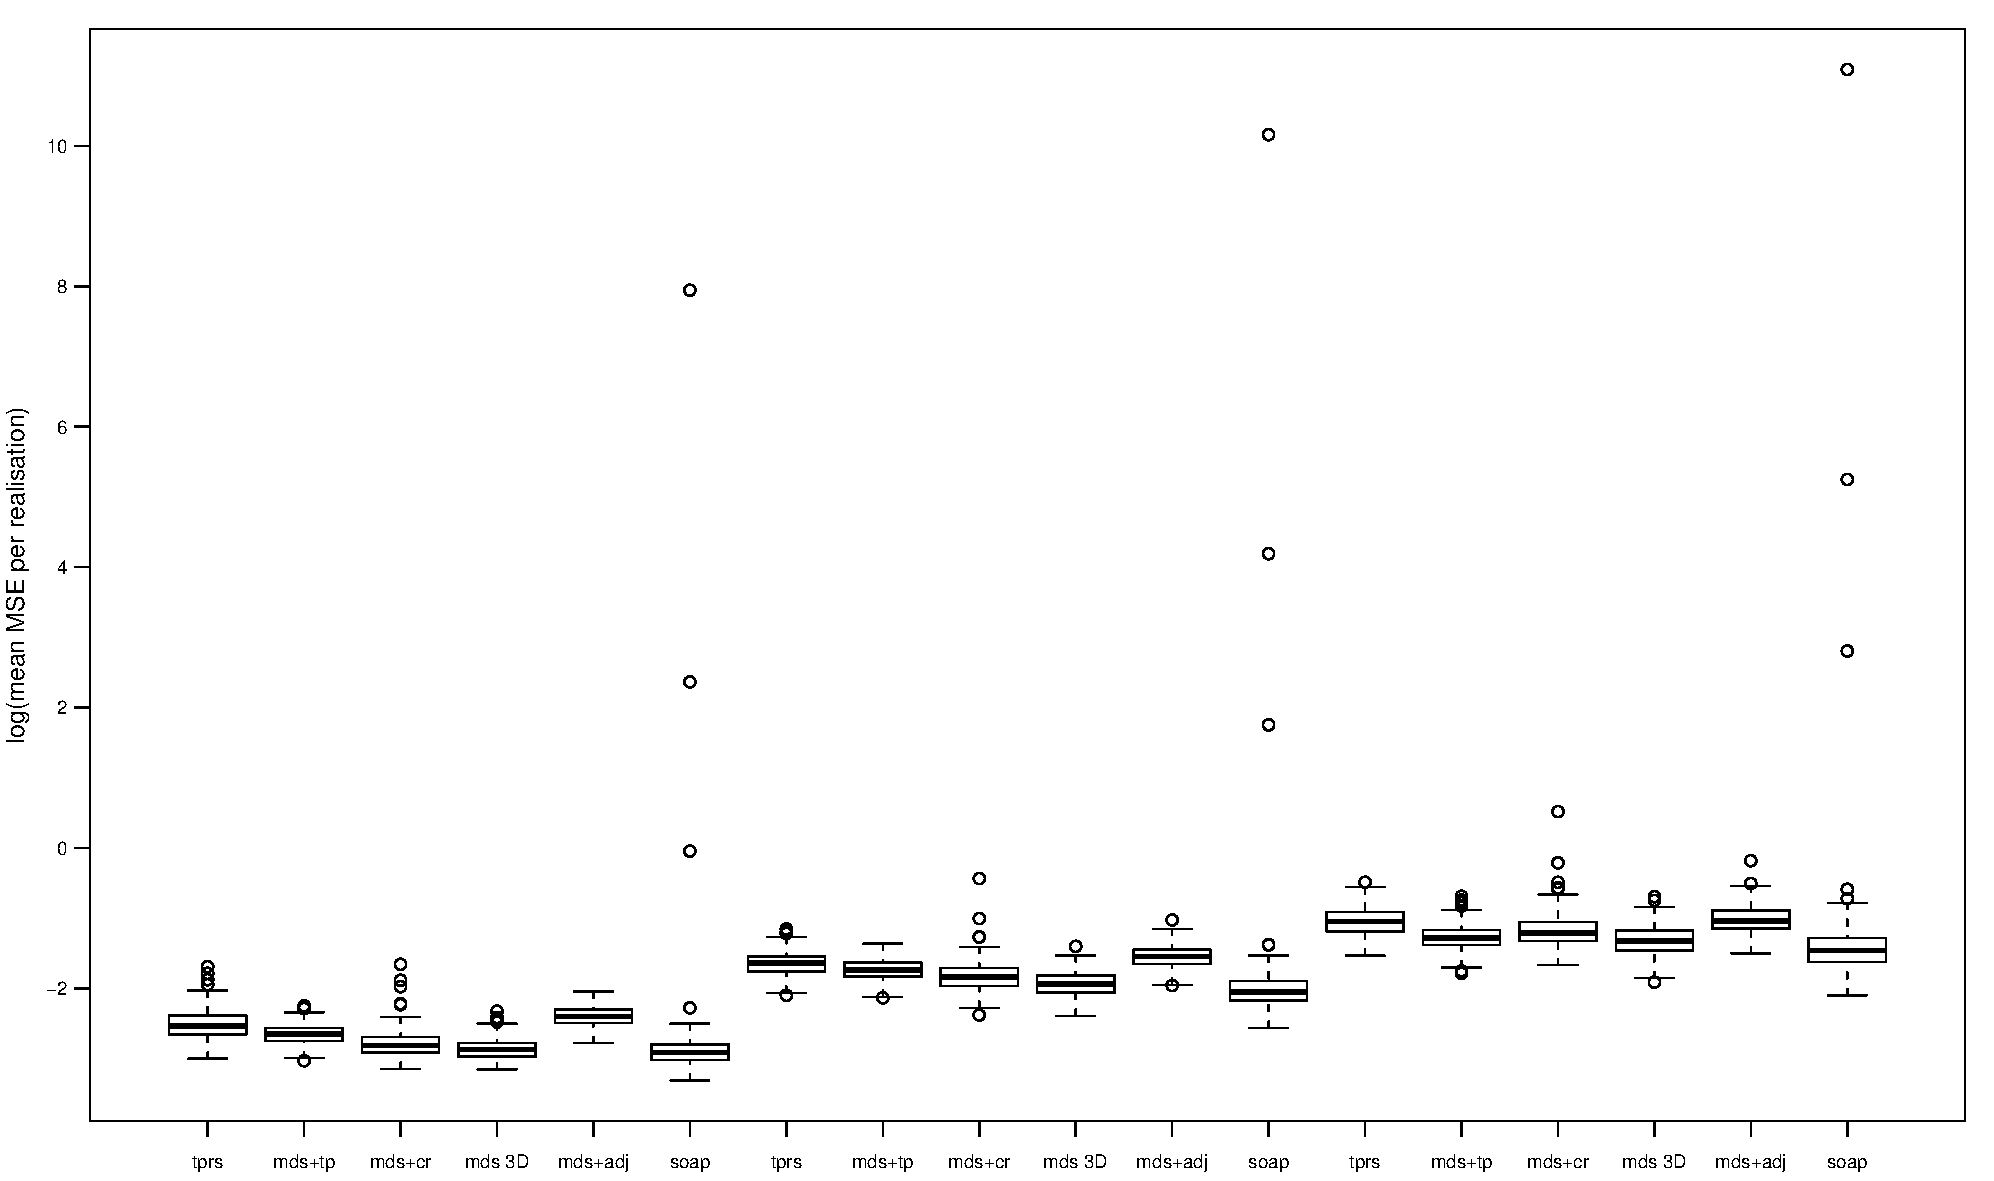
\includegraphics[width=9.5in]{mds/figs/big-mds-wt2-boxplot.pdf} \\
\caption{Logarithm of per realisation average mean squared error for the double peninsulae domain. Models are in groups of six for each error level (0.35,0.9,1.55). In all cases, a Wilcoxon signed rank test showed that MSEs for all models were significantly different from the soap film smoother ($\text{p-value} < 10^{-6}$).}
\label{big-wt2-mses}
% generate /phd-smoothing/mds/sim/boxplot-wt2.R
\end{sidewaysfigure}


\subsection{Aral sea}

The Aral sea is located between Kazakhstan and Uzbekistan. It has been steadily shrinking since the Soviet government diverted the sea's two tributaries in order to irrigate the surrounding desert in the 1960s. The NASA SeaWifs satellite collected data on chlorophyll levels in the Aral sea (\cite{soap}). The 496 data are averages of the $38^\text{th}$ 8 day observation period over the years 1998 to 2002. Smooths were fitted to the spatial coordinates with the logarithm of chlorophyll concentration (with Gamma errors) as the response.

A \tprs, \mdsap\ and soap film were all fitted to the data. In summary the setup for each model was:

\begin{enumerate}
\item \emph{Thin plate spline}:  with basis size 70.
\item \emph{Soap film smoother}: using a 12 by 12 grid of knots (74 were inside) and a boundary smooth with basis size 49.
\item \emph{\mdsap}: with basis size 70.
\end{enumerate}

\begin{figure}
\centering
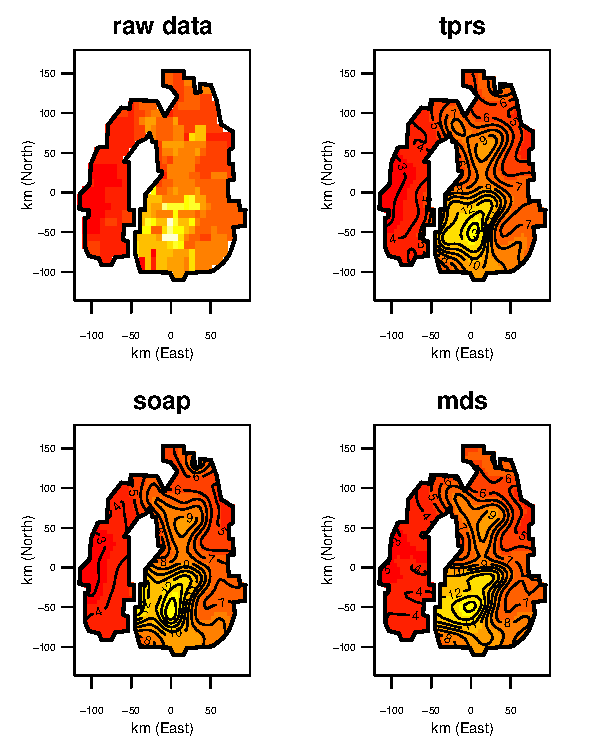
\includegraphics{mds/figs/aral-fit.pdf} \\
\caption{Raw data and predictions from the models fitted to the Aral sea chlorophyll data. Clockwise from top left: raw data, \tprs, soap film smoother, and \mdsap.}
\label{aral-fit}
% generated by phd-smoothing/mds/wt2-intexp.R and intexp/smooth2.c.R with comments removed
\end{figure}

The models were then used to predict over a grid of 496 points to create the heat maps shown in \fig{aral-fit}. The fits are broadly similar, with the \tprs\ showing some signs of leakage around (-50,-50). Both \mdsap\ and the soap film smoother combat this problem. The contour lines for all of the models look roughly the same in the main part of the sea, but in the smaller lobe, \mdsap\ is rather different from both the soap film and \tprs. 

Although the leakage is avoided, there appear to be some strange artefacts in the smooth. Ovals of higher chlorophyll appear in the smaller lobe when the \mdsap\ is fitted to the data, along with contours close to the far left of the smaller lobe. Looking at a point plot in MDS space (\fig{aral-pp}) reveals why this might be happening. As can be seen from the figure, the smaller lobe has been squashed to a line which clearly has an adverse effect on the smoother.

\begin{figure}
\centering
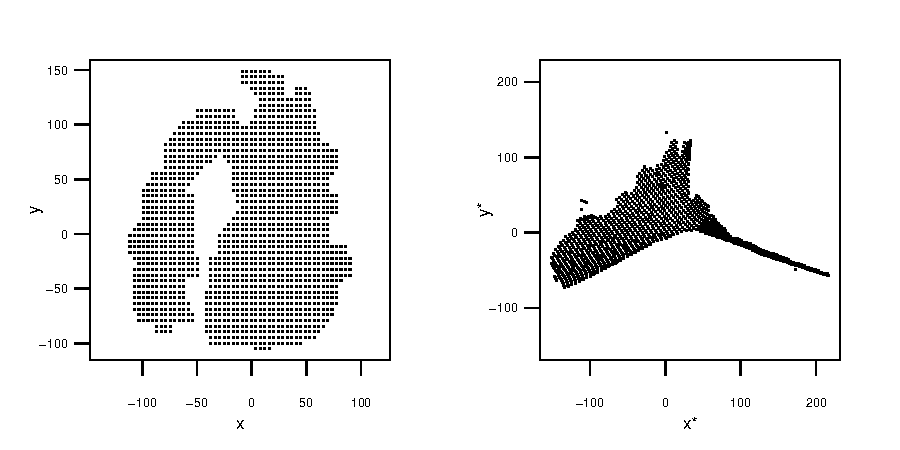
\includegraphics[width=6.25in]{mds/figs/aral-pp.pdf} \\
\caption{The prediction points for the Aral sea data set (left), with their projection into MDS space (right).}
\label{aral-pp}
% generated by phd-smoothing/mds/aral/pointplot.R
\end{figure}

The \mdsap\ with adjusted penalty was also used to fit the model, using the same settings as above. The predicted surface given by the model is shown in \fig{aral-adj-fit}. Again, the same artefacts are clearly visible in the smaller lobe of the region.

\begin{figure}[t]
\centering
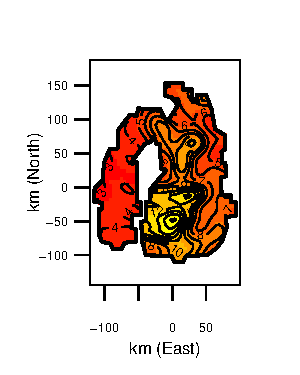
\includegraphics[width=3in]{mds/figs/aral-adjfit.pdf} \\
\caption{Predictions for the Aral sea using \mdsap\ with adjusted penalty.}
\label{aral-adj-fit}
% generated by phd-smoothing/mds/wt2-intexp.R and intexp/smooth2.c.R with comments removed
\end{figure}

Using a 3-D \tprs\ the artefacts are less prominent and the surface looks much more like the one given by the soap film smoother. Again, the three-dimensional projection shows much promise especially given the minimal extra cost to running the additional model (if the within-area distances are already calculated, only the MDS projection needs to be calculated, and the \tprs\ fitted).

\begin{figure}
\centering
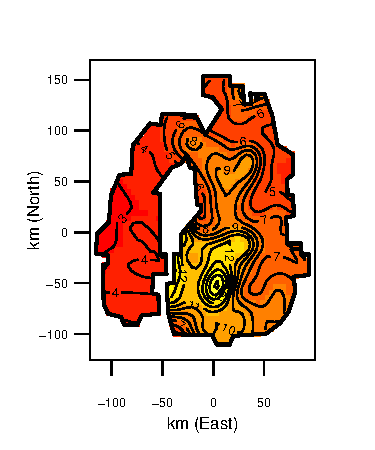
\includegraphics[width=3in]{mds/figs/aral-3d.pdf} \\
\caption{Predictions for the Aral sea using a 3 dimensional projection into MDS space for \mdsap.}
\label{aral-fit-3d}
% generated by phd-smoothing/mds/wt2-intexp.R and intexp/smooth2.c.R with comments removed
\end{figure}

\subsubsection{Aral sea simulation}

The results above show that \mdsap\ does not fit an unreasonable model, but that some artefacts do occur in the predictions. In order to further test \mdsap, a simulation was setup. Truth was set as the predictions given by fitting a kernel regression (using the \textsf{R} package \texttt{np}) to the raw data in \fig{aral-fit}. Bandwidth was selected by expected Kullback-Leibler cross-validation (\cite{hurvich}) using adaptive nearest-neighbours. A local-linear kernel regression estimator was used. 

Taking this kernel estimate as truth (see \fig{aral-np}), samples of size 100, 250 and 500 were taken and noise added from the Gamma distribution with signal-to-noise ratios 0.95, 0.75 and 0.5 (dispersion equal to 6.666,1.265 and 0.9523, and scale equal to  0.4077, 2.495 and 5.748, respectively). Predictions were then made on a grid 1498 points, from this MSEs were calculated and EDFs recorded for each model over 100 realisations.

\begin{figure}
\centering
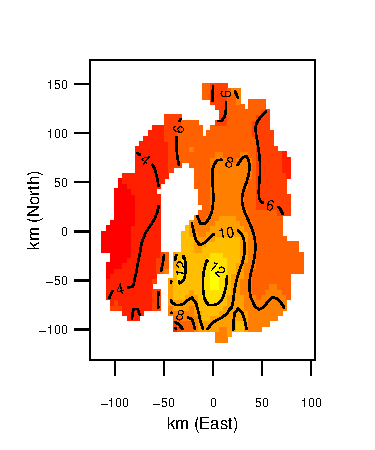
\includegraphics[width=3in]{mds/figs/aral-np.pdf} \\
\caption{The fit given by the kernel regression for the Aral sea, used as truth for simulations}
\label{aral-np}
% generated by thesis/mds/figs/aral-np.R
\end{figure}

The models fitted were as in \secref{wt2bigsim} (but with different basis sizes):

\begin{enumerate}
\item \emph{Thin plate spline}:  with basis size 70.
\item \emph{\mdsap}: using a \tprs\ with basis size 70.
\item \emph{\mdsap}: using a tensor product (see \secref{GAMtensor}) of cubic splines, each dimension of which had a basis size of 9.
\item \emph{\mdsap}: using a 3-dimensional \tprs\ with basis size 70. Here MDS was used to project the data into three dimensions rather than two.
\item \emph{\mdsap}: using a \tprs\ with basis size 70, with penalty adjustments.
\item \emph{Soap film smoother}: using 74 internal knots evenly spaced on a grid over the domain, and a cyclic spline on the boundary of basis size 25.
\end{enumerate}

% big aral sim MSEs
\begin{figure}
\centering
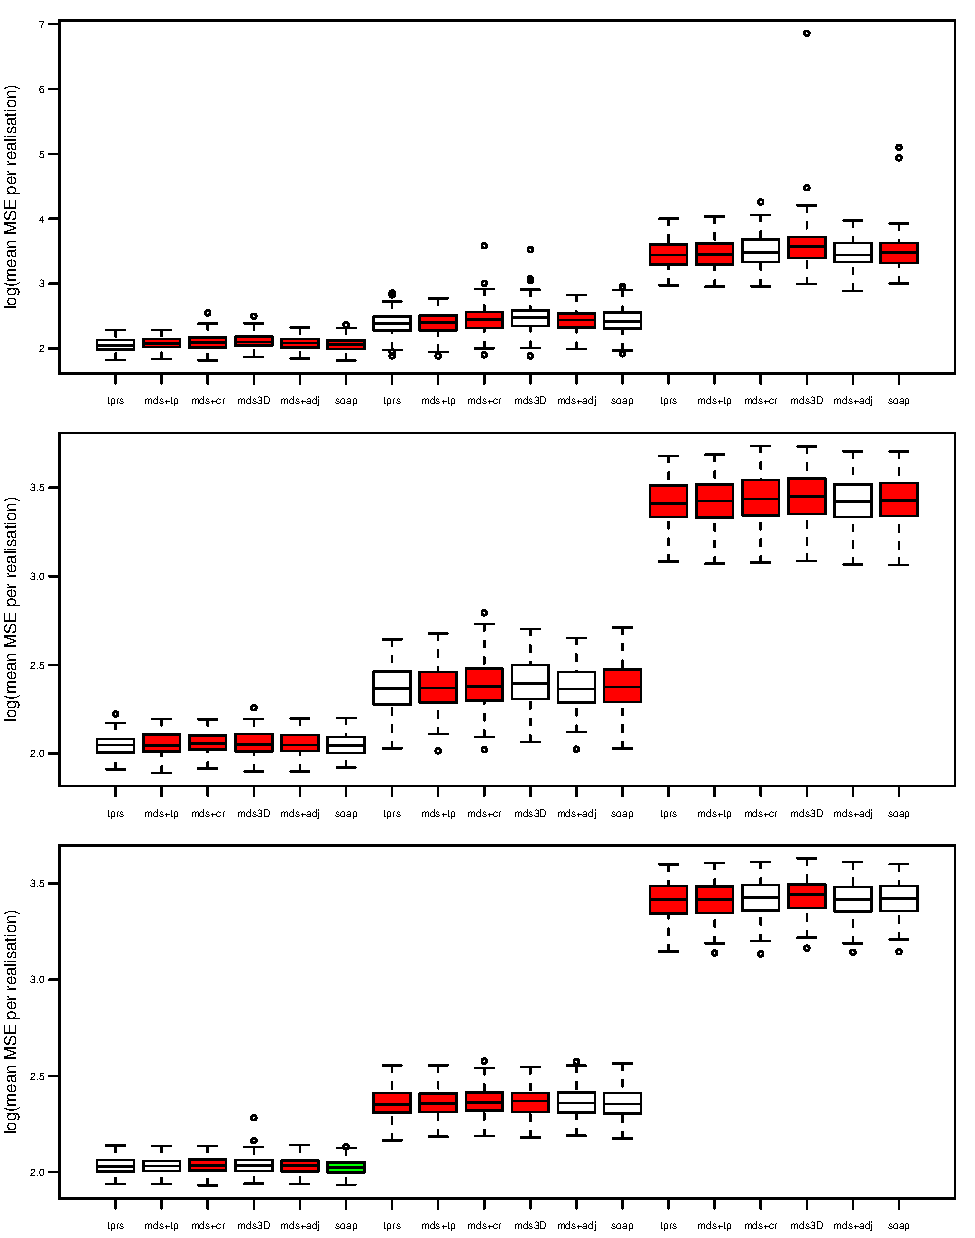
\includegraphics{mds/figs/big-aral-boxplot.pdf} \\
\caption{Box plots of the logarithm of per realisation average mean squared error for the Aral sea simulation. Top to bottom sample sizes: 100, 250, 500. Models are in groups of six for each signal-to-noise ratio (0.95,0.0.75,0.5). The shaded boxes indicate that a Wilcoxon signed rank test showed that there was a significant difference between the model and soap film smoother's MSEs ($\text{p-value} < 10^{-2}$).}
\label{big-aral-mses}
% generate /phd-smoothing/mds/aral/boxplots.R
\end{figure}

\Fig{big-aral-mses} and \tabref{bigaralresultstable} show the results of the simulations. Looking at these, there does not appear to be a clear reason to choose one of the \mdsap\ methods over the others on MSE grounds alone. Perhaps surprisingly, the \tprs\ does rather well in MSE terms, having slightly lower MSE than other models in all situations (although not significantly different from the soap film smoother ($\text{p-value} < 10^{-2}$). This is perhaps to be expected given the leakage was rather slight and localised, this combined with the \tprs\ also fitting a consistently more complex model (see EDFs, \tabref{bigaralresultstable}) may account for the superior MSE. However, we still must prefer the soap film smoother, since it does not allow any leakage. Given the evidence, above, of possible artefacts in \mdsap\ models, the soap film is looking like the best option for smoothing over regions with complex boundaries.

\begin{sidewaystable}[p]
\centering
\begin{tabular}{c c c c c c c c}
 & & &  & MSE  & & &\\ 
 $n$ & SNR & tprs & mds+tp & mds+cr & mds+tp 3D & mds+tp+adj & soap\\ 
\hline
100  &  0.95  & 7.9015 (0.08013) & 7.959 (0.07539) & 8.142 (0.09235) & 8.3365 (0.09319) & 7.9099 (0.07207) & 7.9862 (0.08923) \\ 
100  &  0.75  & 11.1357 (0.20472) & 11.2689 (0.20631) & 11.9138 (0.25673) & 12.2517 (0.24506) & 11.1778 (0.20201) & 11.5665 (0.21725) \\ 
100  &  0.5  & 32.3312 (0.71517) & 32.8335 (0.74064) & 36.3542 (1.82936) & 44.9118 (3.94612) & 32.5586 (0.67499) & 34.7731 (1.59728) \\ 
250  &  0.95  & 7.5986 (0.04417) & 7.698 (0.04591) & 7.7376 (0.04951) & 7.8235 (0.09169) & 7.8895 (0.05065) & 7.6292 (0.04719) \\ 
250  &  0.75  & 10.3526 (0.11208) & 10.5199 (0.11666) & 10.7282 (0.12681) & 10.7975 (0.13027) & 10.9595 (0.12346) & 10.5495 (0.11691) \\ 
250  &  0.5  & 31.1509 (0.4722) & 31.3645 (0.48343) & 32.2298 (0.60102) & 32.6544 (0.54744) & 30.966 (0.40946) & 31.6147 (0.50458) \\ 
500  &  0.95  & 7.6029 (0.03234) & 7.6871 (0.03205) & 7.7303 (0.03395) & 7.6631 (0.03548) & 7.6909 (0.03071) & 7.6072 (0.03209) \\ 
500  &  0.75  & 10.2918 (0.08406) & 10.4119 (0.08297) & 10.5134 (0.08788) & 10.6015 (0.11156) & 10.6991 (0.08454) & 10.373 (0.08497) \\ 
500  &  0.5  & 30.4475 (0.26024) & 30.6894 (0.26375) & 31.0089 (0.26704) & 31.3011 (0.2788) & 30.6516 (0.27123) & 30.8032 (0.26491) \\ 
\end{tabular}
\begin{tabular}{c c c c c c c c}
 & &  & EDF  & & &\\ 
$n$ & SNR & tprs & mds+tp & mds+cr & mds+tp 3D & mds+tp+adj & soap\\ 
\hline
100  &  0.95  & 29.552 (0.87023) & 21.9038 (0.67106) & 18.7032 (0.53711) & 23.254 (0.72225) & 17.3514 (0.45505) & 24.6145 (0.7117) \\ 
100  &  0.75  & 19.491 (0.98279) & 12.8962 (0.56278) & 12.0983 (0.52548) & 13.7002 (0.43143) & 10.6921 (0.34023) & 14.9221 (0.68537) \\ 
100  &  0.5  & 16.5053 (0.91097) & 11.9996 (0.94359) & 11.4546 (0.70547) & 13.7607 (0.51774) & 8.4233 (0.57631) & 12.9575 (0.69218) \\ 
250  &  0.95  & 40.9612 (0.51131) & 33.658 (0.51015) & 28.0043 (0.5445) & 37.5377 (0.63347) & 31.8296 (0.62748) & 38.2715 (0.67473) \\ 
250  &  0.75  & 24.6507 (0.68571) & 19.0361 (0.58564) & 17.6928 (0.64489) & 20.3174 (0.72174) & 17.2911 (0.74521) & 23.2137 (0.76245) \\ 
250  &  0.5  & 19.296 (0.89548) & 14.987 (0.67186) & 12.9415 (0.46289) & 15.3412 (0.6208) & 11.6872 (0.61843) & 18.3504 (1.03563) \\ 
500  &  0.95  & 50.1375 (0.39114) & 43.9809 (0.40286) & 36.0768 (0.57957) & 49.2601 (0.48478) & 42.8032 (0.44318) & 49.6045 (0.76866) \\ 
500  &  0.75  & 31.6271 (0.6354) & 26.8581 (0.72752) & 23.1292 (0.76395) & 29.2308 (0.69282) & 24.762 (0.92098) & 30.0555 (0.7023) \\ 
500  &  0.5  & 25.1535 (0.81385) & 20.7569 (0.89395) & 16.7635 (0.71303) & 20.9786 (0.91157) & 15.8003 (0.79458) & 23.2793 (1.01832) \\ 
\end{tabular}
\caption{Mean MSE and EDF for the six models fitted for the Aral sea simulation with standard errors (in brackets) over 100 realisations.}
\label{bigaralresultstable}
\end{sidewaystable}

\section{Problems with \mdsap}
\label{mds-problems}

\subsection{Why the penalty adjustment sucks}
\label{pensuck}

The simulations show that there is no big advantage of using the adjusted penalty scheme for \mdsap\ over the non-adjusted penalty. Before running the simulations, several different functions of the MDS point density were tried out. All were worse than the function that was finally settled on.

An explanation for why the penalty adjustment doesn't offer much improvement can be found by investigating the good performance of the 3-D projection model. 

Looking at the plots of the prediction points in MDS space for the peninsulae domain (\fig{wt2-2d-proj} and \fig{wt2-3d-proj}) it is easy to see that in two dimensions, the first peninsula has been squashed to a line. This is a result of the truncation performed in the MDS procedure; when we look at the 3-D projection, the peninsula clearly has width, just not in the two dimensional projection. The adjusted penalty attempts to account for this squashing of the points by allowing a more flexible model to be fit in that area. However, what is not taken into account is that some of the points in the peninsula are projected on top of each other or on the wrong side of one another. In other words, the MDS projection makes the points lose their ordering. 

As a simple, unidimensional example, take three points, $a, b, \text{and}\ c$ in the top line of \fig{linedia}. The projection could squash them in the way shown on the second line, in this case the penalty adjustments as described in \cite{wood2000} could be used to correct the model. However, with MDS we can have a situation occurring which is similar to that shown in the bottom line of \fig{linedia}, changing the order of $a, b, \text{and}\ c$. 

In the MDS projection we can see this happening in the peninsula described above. The projection takes a side-on view of the peninsula, making the points lose their ordering. In this case, the penalty adjustment can't save the model. If even the ordering of the points is not guaranteed, then the smoother's job is potentially impossible, especially once these ideas are put into two-dimensions.

\begin{figure}
\centering
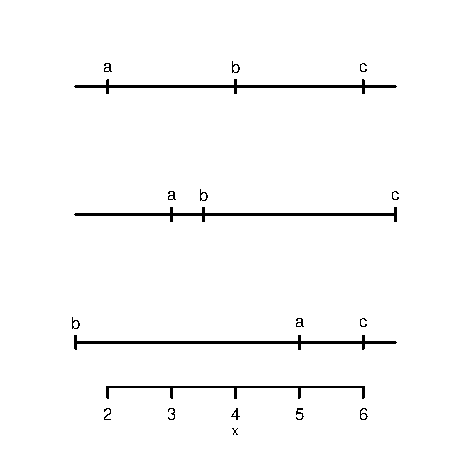
\includegraphics[width=3in]{mds/figs/linedia.pdf} \\
\caption{An illustration of how spatial mappings can squash points (middle line) and reorder them (bottom line) from their original configuration (top line).}
\label{linedia}
% generated by thesis/mds/figs/linedia.R
\end{figure}

\subsection{Why higher dimensions are not the solution}
\label{nohigherdim}

In the two cases above, moving into three dimensions allowed \mdsap\ more accurately reproduce the true function. Counteracting the phenomenon above (where the ordering of the points is lost), the extra dimension allows us to see the ``width'' of part of the domain that we take a side view of the in the 2-dimensional projection.

It seems then that there is some milage to take a 3-dimensional projection to solve this problem without the need for penalty adjustments. However, unfortunately, this is not the case. \Fig{mds-comb} shows a long domain with three peninsulae at each end. The MDS projection of the domain in two dimensions gives the points in \fig{mds-comb-2d}. There are only four peninsulae in this figure, not the six which were in the original. Using the colours in \fig{mds-comb} and \fig{mds-comb-2d}, we can see that the larger peninsulae are separated but not the smaller ones. Assuming that there is some information in the smaller peninsulae and there is reason to believe that leakage would be undesirable, this looks rather bad from a smoothing perspective.

\begin{figure}
\centering
\includegraphics[width=3in]{mds/figs/comb.pdf} \\
\caption{A domain with multiple peninsulae.}
\label{mds-comb}
% generated by thesis/mds/figs/comb.R
\end{figure}

\begin{figure}
\centering
\includegraphics[width=3in]{mds/figs/comb-2d.pdf} \\
\caption{Two-dimensional MDS projection of the domain in \fig{mds-comb}, note that there are only four ``legs'' here not the six that should be there, as in \fig{mds-comb}.}
\label{mds-comb-2d}
% generated by thesis/mds/figs/comb.R
\end{figure}

So, in this case it is not unreasonable to think that an extra dimension could help. Taking a 3-dimensional projection, \fig{mds-comb-3d} is produced, however there is still no separation of the smaller peninsulae. Moving into four dimensions (\fig{mds-comb-4d}) we begin to see separation in the smaller peninsulae. However, the separation is not particularly large and leakage could still happen.

\begin{figure}
\centering
\includegraphics[width=5in]{mds/figs/comb-3d.pdf} \\
\caption{The MDS projection of the domain in \fig{mds-comb} into three dimensions. Note that there is still no separation in for the smaller peninsulae.}
\label{mds-comb-3d}
% generated by thesis/mds/figs/comb.R
\end{figure}

\begin{figure}
\centering
\includegraphics[width=5in]{mds/figs/comb-4d.pdf} \\
\caption{The MDS projection of the domain in \fig{mds-comb} in four dimensions.}
\label{mds-comb-4d}
% generated by thesis/mds/figs/comb.R
\end{figure}

To get a better handle on how well adding dimensions separates the peninsulae, we can use a simple quantitative measure. By comparing the mean square difference between the matrix of within-area distances and matrix of Euclidean distances in the MDS space, we can assess the amount of variation in the within-area distance being accounted for by moving into further dimensions. The criterion is calculated by taking the element-wise difference between the two matrices, squaring them and then taking the mean.

% Results here are in mds/counter/run-DRcomp.R
Looking at this measure for the domain considered in this section (the ``comb''), the Ramsay horseshoe, peninsulae domain and the Aral sea as dimension of projection is increased yields some interesting results. These are summarised in \tabref{increasek}. The table indicates that there is an optimum number of dimensions ($k$) to project into, such that adding a further dimension causes the mean squared difference between the two sets of distances to increase. However, the value of $k$ is not common to all of the domains. Indeed, the Ramsay horseshoe appears to only require two dimensions, where as the peninsulae domain appears to need five. However, we can see that this is by no means definitive, given that for the ``comb'' domain, four dimensions appears to be optimal but \fig{mds-comb-3d} shows that this doesn't offer much separation in the peninsulae.

\begin{table}[htb]
\centering
\begin{tabular}{c c c c c}
$k$ & Comb & Ramsay & Peninsulae & Aral\\ 
\hline
2 & 13.17745 & 0.04260265 & 0.3107145 &  72.4272\\ 
3 & 2.305754 & 0.09755574 & 0.06593825 & 18.87854\\
4 & 2.300667 & 0.1384483  & 0.02818498 & 14.38068\\ 
5 & 2.306849 & 0.1678546  & 0.02293624 & 14.96354\\ 
6 & 2.317045 & 0.2031276  & 0.02439487 & 15.56185 \\ 
\end{tabular}
\caption{Mean squared difference between the matrix of within-area distances and Euclidean distance in a $k$-dimensional MDS projection of the points for each of the domains detailed in \secref{nohigherdim}.}
\label{increasek}
\end{table}

Moving into continually higher dimensions seems appealing, but practically it is rather more taxing. As the dimension of the problem is increased, the order of the penalty in the GAM increases too(see \secref{GAMpenalties}). As this happens, the dimension of the nullspace of the penalty increases, meaning that more functions are unpenalised in the model. This will not lead to a simple model being fitted to the data, the real aim of \mdsap.

\section{\mdsap\ in practise}
\label{mds-prac}

Although \mdsap\ has problems, there may be some cases in which it is useful. For this reason, some practical tips on using the method are given here.

As has been seen in the previous sections, \mdsap\ does have potential pitfalls for the practitioner. Key to the whole method is that the starting grid, used to project the data into MDS space is dense enough so that the features of the domain which cause leakage are captured. In order to make sure that the initial grid is dense enough, a sparse grid over the boundary could be created and gradually made more dense grids until there are only very small changes in the plot of the grid in MDS space. Automation could be achieved by following a similar process (starting with a sparse grid and increasing the density) and at each stage checking to see if the the eigenvalues of the distance matrix have converged.

Choosing a suitable boundary is also essential to making sure that a model can be fitted in reasonable time. The more complex the boundary, the longer the shortest paths will take to calculate. Simplifying the boundary to only include those boundary vertices that are essential to combatting leakage will improve the speed of the fit.

From the analyses above, it is apparent that looking at the plots of the points in MDS space is vital to understanding whether transformation is useful and, in some cases, deciding whether a higher-dimensional projection is necessary.

\section{Conclusion}
\label{mds-conc}

This chapter has investigated the utility of using a combination of multidimensional scaling and penalised regression splines to combat the phenomenon of leakage in spatial smoothing. This was with a view to \mdsap\ being a less complex, faster, alternative to soap film smoothing, with an equally interesting motivating physical model.

As we have seen over the last two chapters, although domain transformation methods are appealing from a mathematical and physical point of view, in practise they do not appear to offer a significant advantage over existing methods and tend to produce artefacts in the resulting smooths.

\mdsap\ has the disadvantage of not calculating a fixed mapping function, as the \sch\ approach did. This leads to a large computational burden when performing prediction over a dense grid. Such an encumbrance is not desirable in a model that gives perfect predictions, let-alone one which has issues with artefacts.

Drawing together what has been learnt from the previous chapters, one can at least begin to create a list of desirable properties which would be required for a domain mapping technique to be useful for finite area smoothing. If a domain morphing technique is ever to work for smoothing over complex regions, the mapping used must have the following properties:

\begin{enumerate}
\item The mapping of points must be smooth, there should be no sudden jumps or gaps. Points that are near one-another in the original space must be near one-another in the transformed space. See (\secref{mds-smoothness}).
\item The transformation must not squash space too much. Squashing points so they are numerically indistinguishable (crowding) must be absolutely avoided, but less severe compressions of space can also cause problems. See (\secref{sch-crowding}) and (\secref{mds-penadjust}).
\item Ordering of points must be maintained. If one thinks of the points in the original space as lying on a grid, the lines joining the points may change length and orientation under the mapping, but must not cross (\secref{pensuck}).
\item A function to map one space into the other must be found. To make the method competitive in terms of computational time, the method must be able to quickly map points from the data space into the smoothing space. This, realistically, can only be achieved by using some kind of functional mapping (\secref{mds-faster}).
\end{enumerate}

Overall, it seems that \mdsap\ is simply not reliable enough to be used in practise. A method that produces artefacts could cause major problems for practitioners, incorrect inference can be extremely damaging in real world situations. The landscape of finite area smoothing over complex regions remains unchanged on the whole, the soap film smoother remains the fastest, most consistent method for performing smoothing in such situations. However, hopefully the criteria above provide some insight for those thinking of using a transformation-type approach in the future.







\chapter{Generalized distance smoothing}
%\begin{quotation}
%The three virtues of a programmer:
%\begin{enumerate}
%\item Laziness - The quality that makes you go to great effort to reduce overall energy expenditure. It makes you write labor-saving programs that other people will find useful, and document what you wrote so you don't have to answer so many questions about it. Hence, the first great virtue of a programmer. Also hence, this book. See also impatience and hubris.
%\item Impatience - The anger you feel when the computer is being lazy. This makes you write programs that don't just react to your needs, but actually anticipate them. Or at least pretend to. Hence, the second great virtue of a programmer. See also laziness and hubris.
%\item Hubris - Excessive pride, the sort of thing Zeus zaps you for. Also the quality that makes you write (and maintain) programs that other people won't want to say bad things about. Hence, the third great virtue of a programmer. See also laziness and impatience.
%\end{enumerate}
%-- Larry Wall, Randal L. Schwartz and Tom Christiansen. 
%\end{quotation}
%\begin{quotation}
%``The three virtues of a programmer: laziness, impatience and hubris.''
%
%-- Larry Wall, Randal L. Schwartz and Tom Christiansen. 
%\end{quotation}


\label{chap-gds}


\section{Introduction}


   what the problems are
   why do it this way (why not use other smoothers)
   

In the previous chapter multidimensional scaling was used to project the points within some geographical area into a new space in which smoothing can be performed without the problem of leakage. However, it has become clear that we face a trade-off in using this method: if the ordering of the points in space is to be maintained (\secref{pensuck}), a sufficiently high dimensional projection of the data must be obtained. Increasing the projection dimension causes the nullspace of the thin plate spline penalty (\secref{GAMtprspenalty}) to become large, causing a large space of wiggly functions to be used without being penalised, leading to unreliable smoothing results (\secref{nohigherdim}). To resolve this issue a smoother which can deal with high dimensional data must be used. 

Smoothing reliably in high dimensions is a difficult problem, however it has been approached in several different ways previously. It is worth quickly covering here other smoothers that could be used to solve this problem and their relative advantages and disadvantages.

WHY DO THESE METHODS SUCK?
\begin{itemize}
   \item Without straying too far from thin plate splines, one could consider using tensor products of splines of any basis (\secref{GAMtensor}). For example, marginal smooths of cubic or P-splines could be combined using a tensor product to create a mutlidimensional smooth in the requisite number of dimensions. Although this approach is appealing conceptually, in practice several problems arise. First is the problem of knot placement (which the thin plate spline neatly avoids, see \secref{GAMtprs}), TKTKTK more here. Second is that tensor product smooths are non-isotropic so the ammount of smoothing in each direction is variable, mutliple smoothing paramater estimation adds further computational burden to the fitting process (TKTKTK cite). Finally, although the marginal functions in a tensor product smooth can be simple, the combination of the functions can turn out to require many evaluations.
   \item Rather than using a fixed basis, one could use LOESS (TKTKTK cite Cleveland 79) which smooths the data using a low-degree local polynomial. 
         as above, in multidimensional case: expensive 
         backfitting only way to integrate with other smoothers
         smoothing selection
   \item GSS
         ???
   \item kriging ???
         covariance matrix stuff -- curriero
   \item kernel smoothing ???
\end{itemize}



If thin plate splines are to continue to be used, the requirement we seek is clear: we wish to smooth in as many dimensions as necessary; but while doing this we must also limit the nullspace of the penalty in order to avoid the side effects of having complicated, unpenalised functions in the resulting smooths. 

In the paper in which thin plate splines are proposed for the first time (\cite{duchon77}) a much more general set of interpolation methods are proposed, of which thin plate splines are a particular example. This chapter illustrates how a more general version of the thin plate spline (henceforth referred to as Duchon splines) can be used for high dimensional smoothing whilst avoiding an overly big penalty nullspace.

The next section goes into the technical detail of how Duchon splines work and how they can be used in the finite area smoothing case. \Secref{gds-wad-examples} shows how this can be useful in the within-area distance case discussed in chapters \ref{chap-sc} and \ref{chap-mds}. \Secref{gds-gds-examples} expands the methodology to look at any problems where distances can be considered, taking the MDS projection of these distances and then smoothing in the projected space. \Secref{gds-software} illustrates the software implementation of these methods. Finally, \secref{gds-conclusion} concludes the chapter.

\section{Using Duchon splines for reliable high dimensional smoothing}

As mentioned above \cite{duchon77} initially proposed a more general version of the thin plate spline penalty and the thin plate spline is just one example of a resulting interpolator. Given that up to this point we have mainly concerned ourselves with thin plate splines and that \secref{GAMtprs} gives explanation of how the thin plate spline works, the following explanation of how Duchon splines operate works from the thin plate spline back to the more general version of the penalty given in \cite{duchon77}. For a more rigorous technical explanation of the construction of such splines, Duchon's paper is recommended.

Beginning with a recap of the physical analogy of the thin plate spline penalty working up to the Duchon spline, the section continues to show how (once reliable high dimensional smoothing can be performed) the size of the MDS projection dimension can be selected.


\subsection{From thin plate splines to Duchon splines}
\label{gds-tprstoduchon}

Going back to the general GAM objective function given in \secref{GAMobjfcn}, we can examine the penalty term. The thin plate penalty in $d$ dimensions with penalty order $m$ is given as:
\begin{equation}
J_{m,d} = \int \ldots \int_{\mathbb{R}^n} \sum_{\nu_1 + \dots + \nu_d=m} \frac{m!}{\nu_1! \dots \nu_d!}\Big( \frac{\partial^m f(x_1,\dots,x_d)}{\partial x_1^{\nu_1} \ldots  \partial x_d^{\nu_d}} \Big)^2 \text{d} x_1 \ldots  \text{d} x_d,
\label{tprs-pen}
\end{equation}
where the summation index generates all of the possible combinations of derivative orders such than their sum is still $m$ (thereby finding all the correct cross-terms). The technical restriction $2m>d$ is also imposed to ensure that $f$ remains continuous.

The thin plate spline is then split into two sets of bases:
\begin{equation}
f(\mathbf{x}) = \sum_{i=1}^n \delta_i \eta_{md}(\mathbf{x}-\mathbf{x_i}) + \sum_{j=1}^M \alpha_j \phi_j(\mathbf{x}),
\label{tprs-basis}
\end{equation}
where the first summation is a series of (local) radial basis functions ($i$ indexing the $n$ data) and the second summation are a set of (global) linearly independent polynomials of degree less than $m$. The terms in the second summation are unpenalised and therefore like in the nullspace of the penalty (\cite{wood2003}). There are $M$ of these polynomials where $M$ is given by:
\begin{equation*}
M=\begin{pmatrix} m+d-1 \\ d  \end{pmatrix}.
\end{equation*}
In the cases presented so far, $d$ (in our the MDS projection dimension) is known and $m$ is dictated by $d$. Increasing $d$ increases $m$ (by the continuity condition that $2m>d$) and hence increases $M$ in the manner above. Therefore $M$ increases very quickly with the number of dimensions used; this is shown in figure \ref{nullspace-dim} (blue line). As more functions are included in the nullspace, the more and more complex (because of their linear independence) the functions are. Having very wiggly functions in the nullspace is certainly undesirable, having many of them will be extremely problematic for model parsimony. 

\begin{figure}
\centering
\includegraphics[width=3in]{gds/figs/nullspace-dim.pdf} \\
\caption{Relationship between smoothing dimension ($d$) and the nullspace dimension ($M$) for thin plate regression splines (blue) and Duchon splines (red).}
\label{nullspace-dim}
% generated by thesis/mds/figs/nullspace-dim.R
\end{figure}

A top-down rigorous proof and treatment of Duchon splines is given in \cite{duchon77}; below is an informal explanation of how from (\ref{tprs-pen}) one can reach the penalty given by Duchon. 

The usual thin plate regression spline penalty given in (\ref{tprs-pen}) can be thought of as a measure of ``wigglyness'' or ``roughness'', taking higher values when $f$ is particularly rough or wiggly (the penalty prevents the spline from interpolating). Integrating the square of the derivatives over the whole of $\mathbb{R}^d$ allows us to consider the fitting procedure as minimizing the objective function in such a way that reduces the wigglyness across the whole of $f$ whilst being as close to the data as possible. 

The penalty in (\ref{tprs-pen}) is only one example of a more general kind of penalty proposed in \cite{duchon77}. Starting from (\ref{tprs-pen}), the first step toward this more general penalty is to consider taking the Fourier transform of the derivatives before squaring and integrating them. The Fourier transform allows us to consider the penalty as an infinite sum of frequencies; decomposing functions defined in space into their frequency domain representations. Mathematically, the Fourier transform of some function of $d$-dimensional space ($\mathbf{x}$), $g$, is defined as:
\begin{equation*}
\mathfrak{F} g(\boldsymbol{\tau}) = \int \ldots \int_{\mathbb{R}^d} e^{2 \pi \sqrt{-1} \mathbf{x}^\text{T} \boldsymbol{\tau}} g(\mathbf{x}) \text{d}\mathbf{x}.
\end{equation*}
Here $\mathfrak{F}$ is an operator applied to $g$, so $\mathfrak{F}g$ may be considered as a function of $\boldsymbol{\tau}$ (a $d$-vector of continuous frequencies). More detail on Fourier transforms can be found in (for example) \cite{bracewell}, \cite{chu-ft} and \cite{beerends}. 

Taking the Fourier transform of the penalty allows us to think of how the penalty is calculated in a different way. Rather than thinking about measuring the wigglyness over the whole of $f$, point by point, instead the measure is based on the frequencies of $f$, the higher the frequency components contribute more to the integral than the lower ones. Intuitively this makes sense, since the low frequency components of the derivatives of $f$ are likely performing a similar task to those functions in the nullspace of the penalty, where as the more complicated, high frequency components are more likely to represent $f$ attempting to interpolate parts of the smooth where consecutive dissimilar values occur.

Taking the Fourier transform of the derivative terms in (\ref{tprs-pen}) yields the following penalty:
\begin{equation}
J_{m,d} = \int \ldots \int_{\mathbb{R}^d} \sum_{\nu_1 + \dots + \nu_d=m} \frac{m!}{\nu_1! \dots \nu_d!}\Big( \mathfrak{F} \frac{\partial^m f}{\partial x_1^{\nu_1} \ldots  \partial x_d^{\nu_d}}(\boldsymbol{\tau}) \Big)^2 \text{d} \boldsymbol{\tau}.
\label{tprs-pen-ft}
\end{equation}
The penalties (\ref{tprs-pen}) and (\ref{tprs-pen-ft}) are in fact equivalent by Plancherel's theorem (\cite{vretblad}, p. 180), so one can take either view and obtain the same numerical value for the penalty.

Since taking the Fourier transform of the derivatives has allowed us to think of the derivatives as made up of frequencies, it then follows to exploit this interpretation by introduing a weighting into the penalty: 
\begin{equation}
\int \ldots \int_{\mathbb{R}^d} w(\boldsymbol{\tau}) \sum_{\nu_1 + \dots + \nu_d=m} \frac{m!}{\nu_1! \dots \nu_d!}\Big( \mathfrak{F} \frac{\partial^m f}{\partial x_1^{\nu_1} \ldots  \partial x_d^{\nu_d}}(\boldsymbol{\tau}) \Big)^2 \text{d} \boldsymbol{\tau},
\label{duchon-penalty-general}
\end{equation}
the function $w$ could then be used to pick out particularly high frequencies and penalise those more than the lower frequency ones. Setting $w(\boldsymbol{\tau})=1, \forall \boldsymbol{\tau}$ allows us to recover (\ref{tprs-pen}).

Duchon shows that if $w(\boldsymbol{\tau})= \lvert \boldsymbol{\tau} \rvert^{2s}$ is used then the thin plate spline functions in (\ref{tprs-basis}) arise. In this case the above penalty becomes:
\begin{equation}
\breve{J}_{m,d} = \int \ldots \int_{\mathbb{R}^d} \lvert \boldsymbol{\tau} \rvert^{2s} \sum_{\nu_1 + \dots + \nu_d=m} \frac{m!}{\nu_1! \dots \nu_d!}\Big( \mathfrak{F} \frac{\partial^m f}{\partial x_1^{\nu_1} \ldots  \partial x_d^{\nu_d}}(\boldsymbol{\tau}) \Big)^2 \text{d} \boldsymbol{\tau}.
\label{duchon-penalty}
\end{equation}
Again, (\ref{tprs-pen}) can be recovered from this penalty (by setting $s=0$). When $s>0$ higher frequencies are penalised more than lower ones. In order to obtain smooth functions it is required that $m+s>d/2$. So $s$ can be used to allow high dimensional smoothing, while still using lower-order penalties without yielding discontinuous functions. One can therefore think of $s$ as a kind of ``fudge factor'' that allows the conditions on $m$ and $d$ to be relaxed; given some fixed combination of $m$ and $d$, an $s$ can be found (by simply calculating $s=d/2-m$).

In a sense, the new penalty allows the radial basis functions in (\ref{tprs-basis}) to fill the gaps left by using a reduced set of global polynomials. Using such a penalty allows us to avoid the problem of having too many complex functions in the nullspace of the penalty while not sacrificing the continuity of $f$. 

Looking back to figure \ref{nullspace-dim} (where the blue line showed the increasing numbers of functions in the nullspace of the conventional thin plate penalty), the red line gives the number of functions in penalty (\ref{duchon-penalty}). In this case $m=2$ has been chosen to remain constant as the dimensionality increases, leading to a linear increase in nullspace size with the smoothing dimension.

\textbf{SIMON} : If I can construct some kind of proof that the MDS projection of within-area distances always leads to a manifold then I'll say something here about how that leads to the following \ldots In any small region a 2-dimensional manifold will look like $\mathbb{R}^2$, in the same small region the smoother's behaviour will closely approximate a regular thin plate regression spline with $m=2$ on the tangent space of the manifold (as the smoothing parameter tends to zero, at least).

These splines have been largly neglected in statistical smoothing literature with the exception of \cite{girosi} which discusses the connections between neural networks and GAMs with the more general form of this type of penalty (ie. (\ref{duchon-penalty-general})). \cite{elements} p. 168 also discuss Girosi's work briefly.

\subsection{Duchon splines with \mdsap\ -- \mdsds}

With the addition of Duchon splines to the \mdsap\ we are now in a position to project data into larger numbers of dimensions and smooth over the response without having to worry about the high dimensional nullspaces causing problems. The use of Duchon splines along with \mdsap\ and the projection dimension selection techniques below will be known as \mdsds\ (Multidimensional Scaling for GAMs) from here on.

\subsection{Choosing MDS projection dimension}

With Duchon's basis, it is now possible to smooth a space of any dimension using a second order derivative penalty, simply by picking $s$ appropriately. Picking the dimension of the MDS projection is now a concern since there is no reason to believe that simply going to higher and higher dimensions will yield better and better results. Keeping in mind the desire for a parsimony, it would be preferable to keep the dimension of the projection as small as possible, whilst avoiding leakage.

\subsubsection{Using proportion of variation explained}

It is clear that as higher and higher projections are used, a larger and larger proportion of the variation in the distance matrix is explained. It therefore seems reasonable to base the choice of dimension on the proportion of the variation explained in the initial grid. However, what proportion should be used? 80\%? 90\%? 99\%? There is no reason to choose any one of these over the others. Setting the proportion of variation to be explained generally is surely a bad idea, since what works for one domain may well be a disaster for another (see also \secref{nohigherdim}).

\subsubsection{Using scores}

Since fitting a GAM with a Duchon spline basis is relatively cheap compared to the cost of finding the within-area distances, the GCV score can be used to find an optimal dimension for the MDS projection. A series of (increasing dimensional) projections can be tried, their GCV scores calculated, and the best selected as the projection to use for the model.

In particular, starting from a 2-dimensional projection, the dimensionality is increased and models fitted, until there is an increase in GCV score. The upper bound is the number of dimensions that explain 95\% (say) of the variation in the distance matrix of the initial grid (see section \ref{grids}).  This favours simpler models (in dimensionality terms), although of course a larger set of dimensions could be considered if there is some prior belief that the dimensionality should be higher or that no clear minima has been found (indeed there is no reason to believe that the GCV score should be unimodal in dimension). It might be considered preferable to take the first minima in the score anyway as we would generally prefer a simpler model. Throughout the following all dimensions between the limits given are assessed to avoid any problems with local optima.

Simulations show that the minima in the GCV score and MSE are in agreement. Figure \ref{wt2-gcv-projdim-boxplot} shows a plot of GCV score and mean squared error for 60 simulations from the peninsula domain, for each of the 60 realisations \mdsds\ was fitted using a 2 through 20 dimensional projection. The boxplots are grouped according to the dimension of the MDS projection used. The graph shows that there is a minima in the score when the dimension is four which corresponds with the minimum MSE.

\begin{figure}
\centering
\includegraphics[width=6in]{mds/figs/wt2-gcv-projdim-boxplot.pdf} \\
\caption{MSE and GCV score for the peninsula domain when different dimensional projections are used. Here a 4-dimensional projection gives a minimum GCV score and MSE.}
\label{wt2-gcv-projdim-boxplot}
% generated by mds/duchon/wt2-gcvml.R
\end{figure}

If smoothing parameter selection is to be performed via ML (\cite{remlpaper}), the ML score can be adapted into an AIC-like score to be used in place of the GCV score, provided there is appropriate penalisation to take into account the increase in the dimension of the projection space. Following score was used:
\begin{equation*}
\text{ML}_p = -2 \hat{l} + 2P
\end{equation*}
where $\hat{l}$ is the log-likelihood at the MLE and $P$ is a penalty which is the nullspace dimension (ie. $M$ from above with $m=2$ and $d$ set to the MDS projection dimension):
\begin{align*}
P =& \begin{pmatrix} 2+d-1 \\ d  \end{pmatrix},\\
=& \begin{pmatrix} d+1 \\ d  \end{pmatrix},\\
=& d+1.
\end{align*}
So the score used to select dimension is:
\begin{equation*}
\text{ML}_p = -2 \hat{l} + 2(d+1)
\end{equation*}
Since the maximum basis is kept constant, but the dimension of the problem changes, this penalty attempts to stop small increases in the likelihood by increasing dimension. This allows the ML score to be used to fit each individual GAM and then comparisons to be made between models of different dimensions. Note the similarity to the AIC.

There is, of course, no guarantee that there will always be a minimum to find and as with all automated methods, practitioners should be mindful of what could potentially go wrong. However, in the situations tested (see below for examples), both of these methods appeared to be satisfactory.

\section{Within-area distance examples}
\label{gds-wad-examples}
\subsection{Simulations}

Returning to the simulation study in section \ref{wt2bigsim}, the same set of simulations (250 samples at three error levels) was re-run using \mdsds, selecting MDS dimension based on both GCV and $\text{ML}_p$ scores (maximum spline basis dimension was set at 100). The results are shown for the original simulations (for thin plate splines and the soap film smoother) along side those for the new model.

Figure \ref{wt2-boxplot-duchon} shows the boxplots for these simulations, \mdsds\ with GCV dimension selection does better than the soap film smoother when the noise is low and was indistinguishable (via a paired Wilcoxon signed rank test) from the soap film smoother at higher noise levels. Using $\text{ML}_p$ gave roughly similar results, becoming significantly different from the soap film smoother at high noise levels.

\begin{figure}
\centering
\includegraphics[width=6in]{mds/figs/wt2-boxplot-duchon.pdf} \\
\caption{Boxplots of logarithm of per realisation average mean squared error from simulations on the peninsula domain. The boxplots are in groups of four for each error level $(\sigma = 0.35, 0.9, 1.55)$. Colours indicate the result of a Wilcoxon paired signed rank test of whether the MSE was significantly (p$<10^{-2}$) different from the soap film smoother. Red indicates different and worse, green different and better.}
\label{wt2-boxplot-duchon}
% generated by mds/duchon/bigsim/boxplot-wt2.R
\end{figure}


\subsection{Revisiting the Aral sea}

Going back to the Aral sea example from section \ref{aral-sec}, we can fit a model using the optimal dimension. Figure \ref{mds-aral-5d-duchon} shows the raw data and a smoothed version, using a 5-dimensional projection (given by minimising the GCV score). The plot does not contain any of the artefacts that were present in the previous smooths of the data.

\begin{figure}
\centering
\includegraphics[width=6in]{mds/figs/aral-5d-duchon.pdf} \\
\caption{The Aral sea chlorophyl levels smoothed using \mdsds, when a 5-dimensional MDS projection is employed. Note the lack of artefacts in comparison to previous \mdsap\ models.}
\label{mds-aral-5d-duchon}
% generated by duchon/aral-evolve.R
\end{figure}

Using the $\text{ML}_p$ statistic to select the MDS projection dimension resulted in a 19-dimensional smooth, significantly greater than the dimension selected by GCV. An image plot is shown in figure \ref{gds-aral-19d}; the produced plot does not look that different from the GCV selected on in figure \ref{mds-aral-5d-duchon}, although it perhaps overfits to the data slightly (for example in the $(-50,100)$ and $(80,-20)$ areas). Figure \ref{gds-aral-dim-select} shows plots of score (both GCV and $\text{ML}_p$) against MDS projection dimension. The GCV plot shows a clear minima where as $\text{ML}_p$ does not. Given this plot and the marginally worse performance in the simulations above, it doesn't seem like $\text{ML}_p$ is a particularly good choice for projection dimension selection when using within-area distances.


\begin{figure}
\centering
\includegraphics[width=4in]{gds/figs/aral-19d.pdf} \\
\caption{Image plot of the smoothed surface fitted by \mdsds\ for the Aral sea when $\text{ML}_p$ is used to select the MDS projection dimension.}
\label{gds-aral-19d}
% generated by duchon/aral-scoreplots.R with liberal use of commenting
\end{figure}


\begin{figure}
\centering
\includegraphics[width=6in]{gds/figs/aral-dim-scores.pdf} \\
\caption{Plots of score against MDS projection dimension for the Aral sea data when GCV (left) and $\text{ML}_p$ are used for dimension selection.}
\label{gds-aral-dim-select}
% generated by duchon/aral-scoreplots.R
\end{figure}

\textbf{SIMON}: do you think I should put some more examples in here? Perhaps a new set of simulations (based on the ``comb'' in section 3.7.2, fig 3-24)?

\section{Generalized distance smoothing}
\label{gds-gds-examples}

Duchon splines are able to smooth in high dimensions without the usual problems that come from such situations. Multidimensional scaling allows the projection of any arbitrary distance matrix into Euclidean space. The combination of these two methods has been successful in the within-area distance case above, but also allows for smoothing using any set of distances.

Data are often collected on scales that are not necessarily physically meaningful (for example in psychological studies or attitude surveys) but the data are used as if the scale was absolute in some sense (\cite{cox2007}, \cite{torgerson}). In such cases the distances between the observations may be meaningful but the actual ordinal values may not be.

Taking data which is either already distances or distances calculated from data, the MDS projection can be found and then a smooth over those data can be used to model some response. Situations where \mdsds\ might be useful fall into three classes: 
\begin{enumerate}
\item Those in which distances are intrinsically meaningful, where distances between the subjects in a study represent some obviously meaningful physical quantity (for example within-area distances in kilometers between observations of whales).
\item Those in which the combinations of variables in the MDS configuration are not meaningful physically but come together to give a measure of dissimilarity between subjects. In this case all of the variables could be of the same ``kind'' (for example, a repeated measure like voting) or could be combinations of measurements of different phenomena (similar to constructed indices used by econometricians from a series of socio-economic variables (household income, education level, state benefit elligability, etc)).
\item Finally, similar to the above class, situations where there are too many variables to be reasonably used in a conventional additive model and therefore using MDS could be used as a variable ``reduction'' technique similar to principle components regression (\cite{elements}, p. 79--80).
\end{enumerate}
The latter two situations pose two interrelated problems. First is that of measurement error: if there are large errors in the variables which are used in the MDS projection, these could unduly influence the result (we usually assume that geographical locations are accurate). For example if there is one very large (erroneous) observation in one of the variables, this could dominate the eigenvalues and cause the variable to have undue prominence in the MDS projection. A thorough treatment of measurement error in non-linear models is given in \cite{measurementerror}. Second is the issue of variable selection; since all variables are used in finding the distances, we have made the assumption that they all affect the response in some way and that the degree to which they have an effect is somehow related to the degree of their variation (or rather, their contribution to the eigenvalues). This is, of course, an unfounded assumption.

Below, the hope is that a combination of appropriate distance metric, projection dimension selection and usual model checking will work around the above issues.

\subsection{Examples}

Data where distances between observations are meaningful can come from many different disciplines. Here two (TKTKTK more?!) examples are given, one from political science and one from biology, however the choice of data here does not indicate any limitation of fields of study to which \mdsds\ can be applied, any discipline in which distances can be measured or calculated \textit{a posteriori} may well benefit from this approach.


\subsubsection{MP data}


The website Public Whip (\url{http://www.publicwhip.org.uk/}) provide data from the Hansard on the votes of 676 MPs in the 1997--2001 Westminster parliament. During this time the House took 1273 divisions. Each vote is coded according to table \ref{voting-code}. Also available from Public Whip are the party allegiances of each MP. 

\begin{table}  
\begin{centering}
\begin{tabular}{ccc}
    Value & Description & Code \\ 
    \hline
    Missing & MP did not vote in this division & 0 \\ 
    Tell aye & MP voted for the motion and was a teller & 1 \\ 
    Aye & MP voted for the motion & 1 \\ 
    Both & MP voted both for  and against the motion & 0 \\ 
    No & MP voted against the motion & -1 \\ 
    Tell no & MP voted against the motion and was a teller & -1 \\ 
  \end{tabular}
\caption{Coding of UK MP voting data. For the purposes of the analysis here the teller's votes are counted as if they voted since we are interested in how voting can be used to predict part affiliation. Note that ``both'' is perfectly possible, and occurs when the MP walks through both the ``Aye'' and ``No'' gates, this can correspond to the MP abstaining (as with ``Missing'') or no nullify a mis-cast vote.}
\end{centering}
\label{voting-code}
\end{table}

Taking the matrix of votes, Euclidean distances between the MPs (rows) were found and used to form the distance matrix. Multidimensional scaling was then used to project these distances into MDS space (dimension selection was performed by optimizing the GCV or $\text{ML}_p$ score). The party affiliation (simplified to Labour party versus not Labour party) was then predicted using a logit link.

Of the 1273 divisions in the 1997--2001 parliament, 17 of them were declared  as ``free votes'' (\cite{freevotes}), where MPs were not ``whipped'' (pressured to take the party line). Predicting affiliation based on whipped votes is relatively easy since MPs are likely to vote along party lines (since they presumably want to keep their leaders happy). Using free votes makes the classification much more difficult. The free votes are summarised in table \ref{free-vote-description}; most of these are ``conscience'' votes.

\begin{table}  
\begin{centering}
\begin{tabular}{cc}
	Date & Bill name \\
    \hline
22 March 2001    &   Election of a Speaker \\
17 January 2001  &   Hunting Bill \\
17 January 2001  &   Hunting Bill \\
17 January 2001  &   Hunting Bill\\
20 December 2000 &   Hunting Bill \\
19 December 2000 &   Human Fertilisation and Embryology\\
31 October 2000  &   Stem Cell Research \\
14 April 2000    &   Medical Treatment (Prevention of Euthanasia) Bill \\
28 February 2000 &   Sexual Offences (Amendment) Bill \\
10 February 2000 &   Sexual Offences (Amendment) Bill \\
28 January 2000  &   Medical Treatment (Prevention of Euthanasia) Bill\\
25 January 1999  &   Sexual Offences (Amendment) Bill\\
22 June 1998     &  Crime and Disorder Bill \\
22 June 1998     &  Crime and Disorder Bill \\
28 November 1997 &  Wild Mammals (Hunting with Dogs) Bill\\
  \end{tabular}
\caption{Free votes in the 1997-2001 parliament (see \cite{freevotes}).}
\end{centering}
\label{free-vote-description}
\end{table}

Using these votes, MPs were selected at random, the model fit to the data and the party affiliation was predicted for those MPs not in the sample. This was repeated for 200 realisations with sample sizes of 200, 300, 400 and 500.

The usual approach for such problems would be to use either a linear model or a variation on the linear model such as the lasso (\cite{elements} pp. 68--69) both using logistic link functions. The built-in function \texttt{glm()} is suitable in the first case and the \textsf{R} package \texttt{glmnet} provides a lasso implementation for the latter.

\textbf{SIMON}: Need to add more detail on the lasso?

The four models tested were:
\begin{enumerate}
	\item \mdsds\ (GCV): MDS projection of the data, selected by minimum GCV score over the full range of 2 to the number of dimensions that account for 85\% of the variation in the sample. Spline basis size maximum was 100.
	\item \mdsds\: ($\text{ML}_p$): as above but using $\text{ML}_p$ score to select the MDS projection dimension.
	\item Lasso: as implemented in \texttt{glmnet}, cross-validation (using deviance as a loss function) was used to select amount of shrinkage per realisation.
	\item GLM: as implemented in \texttt{glm()}.
\end{enumerate}
For all models the error distribution was binomial and a logit link was used.

To compare the results two metrics were used. First the MSE (as defined in \secref{DEFN-MSE}) and second the Brier score (\cite{brier50}). The Brier score is defined as:
\begin{equation}
\text{BS} = \frac{1}{N} \sum_{i=1}^N (\hat{f}_p(\mathbf{x})-y_i)^2
\end{equation}
where subscript $p$ indicates the probability, rather than the prediction on the response scale. The Brier score therefore has the advantage of offering a more granular measure of the accuracy of a model.

\begin{figure}
\centering
\includegraphics[width=6in]{gds/figs/mp-mse.pdf} \\
\caption{Boxpot of MSE per model for the free vote data set at varying sample sizes.}
\label{gds-mps-mse}
% generated by duchon/mps/analyse-mps.R
\end{figure}

\begin{figure}
\centering
\includegraphics[width=6in]{gds/figs/mp-brier.pdf} \\
\caption{Boxplot of Brier score per model for the free vote data set at varying sample sizes.}
\label{gds-mps-brier}
% generated by duchon/mps/analyse-mps.R
\end{figure}

Figures \ref{gds-mps-mse} and \ref{gds-mps-brier} show boxplots of the MSE and Brier scores respectively at the varying sample sizes. The picture painted by the results is consistent across sample sizes, that is that the lasso out-performs other methods. Interestingly, using the $\text{ML}_p$ score rather than the GCV score for the MDS projection dimension yields both a lower median MSE and a smaller standard error. Looking at the plots of score against dimension per simulation (figure \ref{gds-mps-dimselect}), we can see that per simulation (the black lines) the GCV score appears to be much more volatile than the $\text{ML}_p$ criterion. Both scores appear to have a fair spread of selection dimension projections (red dots). Smooths through the full data (blue lines, green confidence bands) do not show that there is any particular, definite minima of the scores in dimension.

\begin{figure}
\centering
\includegraphics[width=6in]{gds/figs/mps-dimselect.pdf} \\
\caption{Plots of MDS projection dimension against score (GCV and $\text{ML}_p$) for the MP voting simulation per sample size. Each line represents one round of cross-validation (some lines are broken due to convergence failure in the GAM), red dots indicate the selected projection dimensions (score minima) per simulation, blue lines are smooths through the full data set and the green bands are confidence bands.}
\label{gds-mps-dimselect}
% generated by duchon/mps/analyse-scoredim.R
\end{figure}

\mdsds\ does not appear to be useful in predicting MPs allegiance using the free vote data. This may be due to there not being enough information in the distances to predict the party; since the data were trinary (votes were coded only $-1$, $0$ or $1$) there would be many distances that were similar. This theory is supported by looking at distance matrix for all MPs for the free votes, in that matrix there are only 63 unique values out of a possible 228150 ($(676*676)-676)/2$ since the matrix is symmetric). Also worth noting is potential confounding between Labour MPs (which made up 429 out of the 676) and other ideologically similar parties (such as Plaid Cymru, SDLP and the Liberal Democrats (at that time)) which might cause potential problems when classifying. This, second, theory is less likely (given how well the lasso and GLM do) but in combination with the first seems plausible.

\subsubsection{Breast cancer microarrays}

Microarrays consist of small silicone or glass chips on which thousands of strands of RNA (which can be thought of as carrying instructions from DNA about how to create proteins) are stuck. These strands are known as \textit{targets} or \textit{probes}. When RNA from the sample comes into contact with that on the chip \textit{hybridisation} occurs (hydrogen bonds between matching parts). The targets are have a fluorescent die applied to them before hybridisation and can be scanned afterward to quantify the number of strands from the sample which have attached themselves to the chip, this is known as the \textit{expression level}.

\cite{ernstbook} (pp. 7--9) describe a data set where both microarray and non-genetic data were collected on 62 patients with breast cancer. Rather than using RNA on the microarray, the experiment used DNA from cancer tissue and measured the differences between the genomic DNA of patients with breast cancer as compared to controls; the theory predicting that cancer causes loss of genetic material or additonal copies of genes to be obtained. The microarray contains expression data on 59 genes. Among the non-genetic data collected was the Nottingham Prognostic Index (NPI) (\cite{Haybittle1982} and \cite{Todd1987}), thought to be a good general measure of prognosis for patients with primary breast cancer (ie. cancer that has not spread beyond the breast). The NPI combines 3 pieces of information in a simple equation
\begin{equation}
\text{NPI} = 0.2(\text{size of index lesion in cm}) + \text{number of lymph nodes} + \text{tumour grade}.
\end{equation}
Further information can be found in the references above; it suffices to say that high values of NPI are bad, identifying those patients with very poor prognoses.

\cite{ernstbook} (pp. 240-245) attempt to predict survival based on microarray data, controlling for other factors. Instead here the NPI is to be predicted based on the microarray data. This is not an unreasonable proposal since if one believes that there is some genetic mechanism behind breast cancer (or at least an individuals vulnerability/resistance to it) then the factors making up the NPI could be considered proxies. 

\cite{spang2002} propose that rather that considering a large number individual genes, combinations are used. \cite{spang2002} use a singular value decomposition of the microarray data to perform dimension reduction. The quantities resulting being referred to as ``super-genes''. In a similar way, using distances between patients and then taking the MDS projection, we can consider ``eigen-genes''.

In section \ref{gds-gds-examples}, above, it was noted that both errors and non-standardised columns in the data matrix can cause issues with MDS since those variables with the greatest degree of variation do not necessarily inform the model the most. One can easily imagine the case in which a completely unrelated gene was measured with huge error and then made up a huge proportion of the first eigenvalue in the decomposition of the distance matrix, this would dominate the projection but contain no information about the prediction (see also \cite{ernstbook} pp. 220-221). To get around this problem, rather than use the Euclidean distance between patients, the Mahalanobis distance (\cite{mahalanobis}) can be used.

The Mahalanobis distance is easily calculated in the following way. If $x_{i.}$ is a single row from the microarray matrix $X$, this represents a single subject. Imagining that subjects are drawn from some multivariate distribution some mean and covariance matrix $\Sigma$, the Mahalanobis distance $d_m$, between subjects $i$ and $j$ is then defined as:
\begin{equation}
d_m = (x_{i.} - x_{j.})^\text{T} \Sigma^{-1} (x_{i.} - x_{j.}),
\end{equation}
where $\Sigma^{-1}$ is replaced with the inverse of the sample covariance matrix of $X$. The calculated distance takes into account that the data may be more variable in some directions than in others. \cite{gentleman2005} suggest using the Mahalanobis distance in a microarray setting.

Calculating the Mahalanobis distance for each pair of patients and putting this into a distance matrix, we can then obtain the MDS projection in the same way as we would with a set of within-area or Euclidean distances.

Of the 62 patients in the study, 45 had non-missing values for NPI and out of the 59 genes in the microarray, 27 did not have missing values. This lead to a vector of 45 NPI measurements and a 45 by 27 matrix for the microarray data. A number of different \mdsds\ models were fitted, with various error distributions. Using standard checks (eg. \texttt{gam.check()} in \texttt{mgcv}, fitting to residuals etc) two were deemed most promising. Those were a model with normal errors and one using a quasi-likelihood (\cite{quasi}, \cite{wood2008}) with a square root link function and variance proportional to the square of the mean. For comparison the lasso (as provided in the \textsf{R} package \texttt{glmnet}) was used. The implementation of the lasso does not allow for quasi-likelihood error distributions to be used, so the normal model for \mdsds\ is a fairer comparison. 

Since the sample size is rather small, it was not possible to reasonably split the data into training and validation sets as with the MP data. Instead, leave-one-out cross-validation (LOOCV) (see section \ref{DEFN-LOOCV}) was used to assess the sensitivity of the models to changes in the data, as well as overall prediction. Table \ref{breast-cancer-cv-results} and figure \ref{breast-cancer-cv-plot} show the results. Both the table and plot show that although \mdsds\ has a lower CV score than the lasso across the board, the variability in the models is about the same.

\begin{table}  
\begin{centering}
\begin{tabular}{cccc}
    Model & Mean & Median & Standard error \\ 
    \hline
lasso                 & 1.67  & 1.021  & 1.837 \\
\mdsds\ (GCV) - normal & 1.41  & 0.695  & 1.759 \\
\mdsds\ (ML) - normal  & 1.426 & 0.629  & 1.873 \\
\mdsds\ (GCV) - quasi  & 1.427 & 0.654  & 1.739 \\
\mdsds\ (ML) - quasi   & 1.419 & 0.575  & 1.857 \\
  \end{tabular}
\caption{LOOCV results for the breast cancer microarray data. Summary statistics are over 45 rounds of cross-validation.}
\end{centering}
% generated by duchon/breast/analyse-cv.R
\label{breast-cancer-cv-results}
\end{table}

\begin{figure}
\centering
\includegraphics[width=6in]{gds/figs/breastcancer-cv-plot.pdf} \\
\caption{Histograms of the CV score per round for the LOOCV of the breast cancer microarray data.}
\label{breast-cancer-cv-plot}
% generated by duchon/breast/analyse-cv-plot.R
\end{figure}

Looking within the \mdsds\ models, we can again look at plots of the MDS projection dimension selection. These are show in figure \ref{breastcancer-dimselect}, where each line represents one round of cross-validation (some lines are broken due to convergence failure in the GAM), red dots indicate minima in the score per simulation (the selected projection dimensions) and the blue lines are smooths through the full data set to give a general idea of what is going on (with green confidence bands). Both error distributions show a similar relationship between dimension and score, however the $\text{ML}_p$ appears again to select high dimensional solutions (in fact all selections were either 19 or 20 dimensions). The GCV score appears to have a fairly clearly defined minima. 

\begin{figure}
\centering
\includegraphics[width=6in]{gds/figs/breastcancer-dimselect.pdf} \\
\caption{Plots of MDS projection dimension against score (GCV and $\text{ML}_p$) for both normal (left) and quasi-likelihood (right) models for the breast cancer microarray LOOCV. Each line represents one round of cross-validation (some lines are broken due to convergence failure in the GAM), red dots indicate the selected projection dimensions (score minima) per simulation, blue lines are smooths through the full data set and the green bands are confidence bands.}
\label{breastcancer-dimselect}
% generated by duchon/breast/analyse-dimselect.R
\end{figure}

In this example we have seen that \mdsds\ is capable of being used for generalized distance smoothing in a microarray setting when Mahalanobis distances are used in place of Euclidean. It would be interesting to investigate the behaviour of the $\text{ML}_p$ score further on larger data sets (since although it picks very high dimensional solutions, their CV scores are lower). The study here is rather small and specialized, therefore it is hard to draw a conclusion about how \mdsds\ will perform in other situations, although its performance here against the lasso (technique that has been in development for considerably longer) is encouraging.

\subsubsection{Leukemia microarrays}

\cite{yeoh2002} investigate expression data from 327 patients with acute lymphoblastic leukemia (ALL), collected on 12626 genes. The orginal purpose of the study was attempting to classify patients into one of ten prognostically important ALL subtypes (since treatment is dependent on subtype), based on looking at the expression data. \cite{yeoh2002} used heirarchical clustering to find groupings of genes in the data and then found those groups corresponded to particular ALL subtypes. Genes were ranked per subtype according a $\chi^2$ statistic (based on the expected value per cluster) to find the most relevant genes for each subtype (more information may be found at \url{http://www.stjuderesearch.org/data/ALL1}).

To simply the analysis here, a binary response was used (of a particular subtype versus not that subtype). Two subtypes were used in the simulation, TEL (the largest group, with 79 patients) and T-ALL (a smaller group with 43 patients). For each subtype two simulations were ran, one using the 40 genes selected by $\chi^2$, and a second that used an additional 500 genes which were chosen at random (but were kept the same over realisations). The two scenarios show the difference between an idealised situation where the best predictors are already know versus a more realistic situation in which there is a lot of noise from non-relevant genes. In each of the simulations 100 realisations were generated and in each of these 100 samples were taken and models fit using their data. Models were then used to predict the classes of the remaining patients, Brier scores and MSEs were recorded. Models using both ML and GCV dimension selection were used and as above, the lasso was used for comparison using the same settings as in the MP example. 


one with just the 40 genes found by chisq


RESULTS

TKTKTK OTHER STUFF
   unlikely given that using correlations alone 96\% accuracy ! that's just linear
   remove linear models


\section{Software implementation - \mdspack}
\label{gds-software}

The methods detailed in this section, namely the use of Duchon splines along with MDS to perform smoothing are provided in the \textsf{R} package \mdspack\ which is available at\ldots

TKTKTK writeup once properly integrated with mgcv and user interface is nicer.

TKTKTK write documentation in the package


\section{Conclusion}
\label{gds-conclusion}

TKTKTK sum up, say what else could be done. Show path SC->MDS+RS->MSG, improvements along the way.

TKTKTK write about interpretability of GDS results, mainly data mining rather than inference (cite Breiman two cultures paper?). IS IT EVEN GOOD AT THIS??!



\chapter{Conclusion}
\label{chap-fasend}

This chapter draws to a close the smoothing part of the thesis. It first compares the methods set forth here with the kriging methods alluded to in \secref{intro-leakageapproaches}, it then goes on to give information about the software implementation of the models discussed so far. Finally, the work from the last five chapters is summarized and further work proposed.

\section{Comparison with MDS-based kriging\\methods}
\label{gds-krig}

Kriging is focused on the explicit modelling of the correlations between points in space as a function of the distance between them via the estimation of the semivariogram. It is therefore logical that in, say, a river system the distances between points are calculated along the river's course rather than the Euclidean distance. 

For the semivariogram to be a valid covariance function, it must be positive definite or conditionally negative definite (see \cite[p. 47]{diggle} for more information). However when non-Euclidean distances are used the semivariogram may no-longer fulfil either of these conditions (\cite{curriero}). The work of \citeb{mdskrig} attempts to solve this problem by using multidimensional scaling to project water distances into Euclidean space. Distances are not found exactly: a series of approximations are used rather than directly calculating the distances between the data. First the domain in question is triangulated, then the ``river distance'' between all of the notes in the triangulation are calculated via Dijkstra's algorithm. The river distances are then projected using MDS. Finally, the data locations are mapped into the MDS space by interpolating between the grid points from the triangulation in MDS space.  The Euclidean distances in MDS space are then used in the estimation of the semivariogram. There are a number of issues with this approach. 

Most prominently, the authors only consider ordinary kriging (where the mean process is treated as constant). In this case spatial variation only enters the model through the semivariogram.The effect of using the MDS projected points for a spatially varying mean process (in addition to the estimation of the semivariogram) has not been investigated. Prevailing opinion is that only polynomial trends should be used for the mean process (\cite[p. 57]{diggle}), how such an approach would perform in higher dimensions is not clear.

Although the approximations used undoubtedly decrease the computational time, the validity of the approximations is not tested (especially on the fitting of the semivariogram, \cite{crabkrig}). The discretisation of the domain necessary to compute the graph distance via Dijsktra's algorithm has similar pitfalls to \citeb{wangranalli}. \citeb{crabkrig} suggest using the proportion of variation explained or the Bayesian criterion of \citeb{ohraftery} as possible metrics to perform projection dimension selection but do not full address the issue, resorting to 2-dimensional projections. Neither of the proposed selection methods take into account the effect that the dimension of the MDS projection has on the overall model (as discussed in \secref{gds-dimselect}).  \citeb{boisvert} suggest that to best approximate the distances, an $n-1$ dimensional projection of the distance matrix (if there are $n$ data, or triangulation nodes) be used (which is of course true) however they go on to point out that the use of such a high-dimensional projection could lead to numerical issues. Interpolating to find the distances in higher dimensions may also have it's own issues and so the approximations may run into further problems. In all of these works the MDS projection is being used to approximate the within-area distances by a set of distances obeying the rules of a Euclidean metric (the criterion given by \cite{curriero} to ensure valid semivariograms). Unlike in the material presented here, the MDS point configuration itself is not being used except to obtain the distances to estimate the semivariogram.

In general kriging methods suffer from having developed as an \textit{ad hoc} set of tools used in the mining industry (\cite[preface]{diggle}). Although much work has been done to improve the mathematical basis of kriging, models are not as flexible as GAMs, in particular the incorporation of other covariates, temporal effects and random effects is not straight forward as it is for additive and generalized additive models (in both theory and practise).

\section{Software implementation - \mdspack}
\label{gds-software}

The methods detailed in this first part of the thesis: the combination Duchon splines and MDS to perform smoothing (along with the within-area distance algorithm) are provided in the \textsf{R} package \mdspack\ (MultiDimensional Scaling for GAMs) which is available at \url{http://www.github.com/dill/msg}. Documentation is provided in the package and has been designed to be familiar to users of \texttt{mgcv} (\mdspack\ implements the methods detailed here as an extra basis for \texttt{mgcv} so minimal code changes are needed to try \mdsds\ on existing problems).

\section{Finite area smoothing conclusion}
\label{gds-conclusion}

This part of the thesis started by introducing additive and generalized additive models and the problem presented when smoothing in a finite area when the boundary is a complex shape: leakage. Current approaches to the problem were then reviewed. Chapter \ref{chap-it} then illustrated the methods of the first in practise. Based on the work in \citeb{miller2011}, the first application of the soap film smoother to model spatiotemporal data (via a tensor product formulation) was presented.

Chapters \ref{chap-sc}, \ref{chap-mds} and \ref{chap-gds} developed two transformation-based methods to combat leakage. At each stage of the work presented in this thesis the models became more refined and a more nuanced view of how the problem should be addressed was developed. Moving from a strictly functional mapping based on the boundary (the \sch\ transform) to one that preserves within-area distances (MDS) was key to finding a reliable transformation that avoided the artefacts caused by the squashing of space. The discovery that the point configurations produced by MDS can cause the ordering of the points to be lost in 2-dimensions explained the poor performance of the model up to that point. The final breakthrough was understanding that by projecting into higher dimensions, the ordering problem can be avoided and that by using Duchon splines reliable high dimensional can take place. This final model, \mdsds, performed very well in simulation, rivalling the soap film smoother.

As well as developing a method which is competitive with the current ``best'' (the soap film smoother), the investigations in the previous chapters have also revealed a set of essential and a set of disirable properties for transformation methods if they are to be used to perform spatial smoothing. The essential properties are:
\begin{enumerate}
\item The mapping of points must be smooth, there should be no sudden jumps or gaps. Points that are near one-another in the original space must be near one-another in the transformed space (\secref{sc-conclusions}).
\item The transformation must not squash space too much. Squashing points so they are numerically indistinguishable (crowding) must be absolutely avoided, but less severe compressions of space can also cause problems (\secref{sch-crowding} and \secref{mds-penadjust}).
\item Ordering of points must be maintained. If the response values are mis-ordered then modelling becomes impossible (\secref{pensuck}).
\end{enumerate}
As well as the above, there are other non-essential but desirable properties:
\begin{enumerate}
\item To make the method competitive in terms of computational time, the mapping of points from the domain of interest into the transformed space must be fast. This can be achieved by using some kind of functional mapping (chapter \ref{chap-it}) or by a sufficiently optimizing the procedure (\secref{mds-faster}).
\item Being able to integrate the spatial smooth into a larger model incorporating covariates, temporal interactions and random effects is extremely useful in practise (chapter \ref{chap-it} and \secref{gds-krig}).
\item Creating a method which appears to be familiar to the practitioner, will make the model building process much more streamlined. Combining this with a software implementation in a standard environment with a well-known paradigm can only help users (\secref{it-conc}).
\end{enumerate}

The methods proposed in chapters \ref{chap-sc} and \ref{chap-mds} do not fully achieve all of these goals, however the work in developing them did help to form the above lists. 

Moving on to further work, the speed of the algorithm for finding the within-area distances is still an issue, although there are several relatively simple tweaks that would make it faster. Finding schemes for the layout of starting grids and perhaps adapting the methods described in \citeb{mdskrig} to approximate the distances using a triangulation, would certainly increase performance (although perhaps at the price of accuracy).

As it stands distance generation is seen as a black box procedure to the model. This means that any procedure that can generate a distance matrix can be used. Aside from the discrete space approximation algorithms mentioned in \secref{mdsdist}, other measures can be used while still keeping in a roughly spatial context. One interesting approach would be to use distances in three dimensions, finding the shortest path over say a mountain range, which would include minimizing changes in altitude as well as avoiding obstactles. Alternatively, a cost based distance approach that takes into account fuel cost or taking into account difficult conditions (e.g. a bog or ford that can be crossed but at additional cost in terms of effort or time). One issue with such general cost-distance approach might be that the ``distance'' measure could turn out to be non-metric. That is, that the distance from A to B is not the same as the distance from B to A (for example going against versus going with the flow of a river). In this case non-metric MDS must be used, this relies only on the rankings of the data and discards other information, which is probably undesirable.

The examples presented here only consider smoothing inside of simple polygons since the within-area distance algorithm given in \secref{mdsdist} can only find shortest paths inside such shapes. This excludes domains with islands in them, which obviously occur in ship-board studies. This could be worked-around using other shortest path algorithms, however the behaviour of MDS (especially in higher dimensions) in such situations is unknown.

Even given its limitations, \mdsds\ does still show an improvement over the soap film smoother in MSE terms, as well as producing reasonable-looking maps in situations with real data. Only further testing on more data sets will show the limitations and the strengths of \mdsds, for now the method appears to be a useful addition to a practitioner's toolkit.

\section{Generalised distance smoothing conclusion}
\label{fasend-gds-conc}

The last chapter discussed smoothing in a more general setting, using MDS to project a matrix of dissimilarities that were not spatial in nature. Using general distances is appealing since most measurements have an arbitrary zero point (with the exception of some physical quantities like temperature). What is really of interest in most situations is the differences between the observations and using these quantities directly makes sense. This is especially true in medical studies since there is evidence that those who are genetically similar are at risk of the same diseases, even if it is not known which genes in particular are indicators of the disease.

Despite the appeal of such a modelling strategy, problems arose. These centred on the choice of distance measure to be used. Choosing certain metrics gave better results than others, so the selection of the metric was down to trying many different options and seeing which was best (in the cases considered here, in terms of MSE, LOOCV or Brier score). The lack of any kind of continuum for the various possible distance measures means that a combination subject specific knowledge and trial and error must be used (rather than automation) to find the appropriate distance measure.

Even if a ``correct'' distance measure can be found, there is no guarantee that the resulting model will capture the key features of the data. This is due to the nature of MDS, as touched in section \ref{gds-gds-examples}. MDS is based on taking the eigen-decomposition of the distance matrix, then using those eigenvectors with the largest eigenvalues to represent the points. Those directions with the largest eigenvalues are not necessarily those with the best predictive power. Using scores to select the number of dimensions overcomes this to some degree but because of the hierarchical nature of the projection only the number of dimensions can be selected. Of course, one could imagine the situation where the full MDS projection was found (in, say $n-1$ dimensions) and then variable selection could be performed on all of the possible combinations. This is not appealing if only because the computational burden of performing the necessary subset selection. Using a full projection also rather subverts the point of the MDS, it would surely be easier to use a more traditional variable selection technique in that case.

In the examples in the previous chapter, the aim of using general distance smoothing has been to perform dimension reduction. However, in the finite area case the idea is to embed further information (about the boundary) into the distances, two approaches are rather different. In the finite area case the MDS projected coordinates not only contain information about the position of the points in space in relation to one another, but also their position with respect to the boundary: the within-area distance algorithm and MDS procedure have imbued the points with extra information. However, in the general distance case the idea is to discard the data which is not useful, a rather different objective and one that \mdsds\ does not appear to excel at.

Finally, the issue of interpretability arises. Even if \mdsds\ in the general distance setting were able to outperform the lasso in MSE terms, the model would be able to do only that. Interpretability is not \mdsds's strong suit, even plotting the results is difficult. It could however be used as in the finite area case, as a smoother to remove some kind of autocorrelation in the data (perhaps if genetic data could be used in a similar way to spatial data in a larger model), as a smooth that is not of main scientific interest but is never-the-less useful to the process of model building. A simple interpretation of these smooths however, seems out of reach.

\section{Conclusion}

This first part of the thesis has developed a transformation-based method for dealing with the problem of leakage in finite area smoothing. The physical model behind \mdsds\ is appealing since it does what one would intuitively want to do with a domain with a complex boundary: pull apart those areas of the domain that unduly influence one another. The final model presented in chapter \ref{chap-gds} performs at least as well in a spatial setting as the soap film smoother.

The key developments in this parts of the thesis are:
\begin{enumerate}
\item First application of the soap film smoother as part of a spatiotemporal model (chapter \ref{chap-it}).
\item Rejection of the \sch\ transform as a method for domain transformation, due to its propensity to overly squash together points in the resulting domain (chapter \ref{chap-sc}).
\item A new algorithm for finding distances between points in simple polygons (chapter \ref{chap-mds}).
\item Development of a domain transformation method to avoid leakage in finite area smoothing based on preserving within-area distances using multidimensional scaling. Subsequently that when using multidimensional scaling in this context that low dimensional projections of points can cause a loss of order which is detrimental to smoothing (chapter \ref{chap-mds}).
\item Application of Duchon splines to avoid the problems associated with thin plate regression splines when performing high dimensional smoothing and use of GCV and REML scores to determine the necessary multidimensional scaling projection dimension in a spatial setting (chapter \ref{chap-gds}).
\item A general method for smoothing dissimilarities using multidimensional scaling to project the data (chapter \ref{chap-gds}).
\end{enumerate}

Further work includes adapting \mdsds\ to work in more complex domains (like non-simple polygons), applications to a wider set of domains and an investigation of utility of the method in larger models. The further development of the generalized distance smoothing ideas in the last chapter may prove extremely useful provided that the issues surrounding the choice of metric can be addressed (particularly in a medical setting). For now it is hoped that \mdsds\ becomes a useful tool for those performing spatial modelling in complex domains.



\part{Distance sampling}

\chapter{Introduction to distance sampling}
\label{chap-intro-ds}

\label{intro-DS}

Distance sampling (\cite{IDS}, \cite{ADS}) is a popular method for estimating the abundance of biological populations. It has been used by researchers across the globe to assess the abundance of everything from birds nests to marine mammals. Surveys are cheap to run since they do not require many observers (unlike a census) or multiple site visits (unlike mark-recapture). Distance sampling is also rather different from methods like mark-recapture (\cite{ruthbook}) as it does not explicitly include the abundance in the likelihood, as shall be seen below. The popularity of distance sampling is in part due to the software Distance (\cite{distance-software}) which makes it easy to record and analyse distance sampling data. 

\section{From quadrat sampling to distance sampling}
\label{quad2ds}

One can think of distance sampling as the logical extension of quadrat and strip transect sampling. In quadrat sampling a series of squares (quadrats) are laid out at random over the sample area and the number of objects of interest within each is counted. It is assumed that within each quadrat a census is performed. From the per-quadrat abundance the density is estimated and multiplied-up to find the total abundance. For quadrat sampling to be efficient the quadrats need to be large and hence it is almost impossible to ensure that all objects in the quadrat are seen, this can be further hindered by animals moving between the quadrats during the survey (\cite[p. 2]{IDS}).

% evolution to DS from quadrat and strip
\begin{figure}
\centering
% trim order l b r t
\includegraphics{intro/figs/quadrat-to-ds.pdf}\\
\caption{An example of quadrat sampling (left), strip transect sampling (middle), and distance sampling (right). Dots indicate individuals, red dots are observed individuals, black those missed. In the first two cases, the grey boxes represent the sampling units. Note that there are many observations just outside of the boxes, which cannot be recorded by survey staff. In the distance sampling case, the solid vertical lines represent the transects and the dashed line gives the effective strip width. Distances are shown by the solid horizontal lines.}
\label{quad-to-ds}
\end{figure}

To make the task of counting the objects within the quadrat easier, one could modify the square design to be a long strip, so that the observer could walk down the centreline of the strip, observing those objects within the strip. Mathematically, if we let the each strip be of width $2w$ ($w$ either side of the line the observer walks down) and the sum of all strip lengths be $L$, if $n$ objects are observed we have a simple estimator of the density, $D$:
\begin{equation}
\hat{D}=\frac{n}{2wL}.
\label{ds-simpleD}
\end{equation}

The problem with both quadrat and strip sampling is that there may well be many objects just outside of the covered area. Clearly this is a waste of survey effort, since observers must ignore objects that they have seen but that are not within the strip. It would be preferable to include as many observations as possible and leverage the maximum amount of data that can be collected to assess the abundance of the population.

Distance sampling is based on this principle; if the objects of interest are seen, then their presence should be recorded. Instead of using fixed-area sampling units, distance sampling requires that only centrelines are specified. The observers should walk (or swim, ride, drive, sail, etc) down the centrelines recording the distances ($x_i$) to the observed objects as they go. Once the survey is complete, the distances are used to estimated the effective area that was sampled. Figure \ref{quad-to-ds} shows the evolution from quadrat to strip to distance sampling.

In equation (\ref{ds-simpleD}) one can think of replacing $w$ with an estimate of $\mu$, the \textit{effective strip (half-)width}. This is the distance at which as many animals were detected beyond as there were missed inside. Further explanation of $\mu$ is given in \secref{gtoD}, but it serves for now to say that by replacing $w$ with $\mu$ an estimate of the area that was effectively surveyed can be found. (\ref{ds-simpleD}) can then be modified to:
\begin{equation}
\hat{D}=\frac{n}{2\hat{\mu}L}.
\label{ds-D}
\end{equation}
We could also consider that a certain proportion ($\hat{p}$, the probability of detection) of the objects in a fixed-area ($2wL$) were sampled, so the above can also be expressed as:
\begin{equation*}
\hat{D}=\frac{n}{2wL\hat{p}}.
\end{equation*}
Here $w$ is the point after which observations are discarded and is referred to as the \textit{truncation} distance. Truncation is used to discard outliers that make the estimation process tricky (\cite[pp. 15-16]{IDS}). From these two expressions we can see that the relationship between $p$ and $\mu$ is $p=\mu/w$, these quantities will be investigated further below.

A typical example of line transect data is shown in figure \ref{ds-lt-example}. The figure shows a histogram of perpendicular distances. Note how, as distance increases the number of detections decreases. This characteristic will be exploited later.

% example of line transect data
\begin{figure}
\centering
\includegraphics{intro/figs/ds-golftee.pdf}\\
\caption{A histogram of line transect data. In this case from an experiment conducted at the University of St Andrews. 760 golf tees were randomly distributed over a 1680m$^2$ area, then observed in 11 transects by 8 independent surveys. Further detail may be found in \citeb[p. 140]{ADS} and \citeb{yellowbook}.}
\label{ds-lt-example}
\end{figure}

\subsection{Point transects}
Line transects are not the only way of collecting data for a distance sampling analysis; point transects may also be used. When using point transects the observer stands at one of a series ($m$, say) of points and observes the objects surrounding him/her. Again, distances to the objects ($r_i$) are recorded. An \textit{effective radius} ($\rho$) is then calculated (analogously to $\mu$) and then object density can be estimated by\label{cor-7s1}:
\begin{equation*}
\hat{D}=\frac{n}{m \pi \hat{\rho}^2}=\frac{n}{m\pi w^2\hat{p}}.
\end{equation*}
The relation between these quantities will be explained below in \secref{gtoD}.

An example of point transect data is given in figure \ref{ds-pt-example}. In contrast to the line transect case, there are very few observations near 0, they increase to a point and then fall off beyond that. Note that as the distance, $r$, from the observation point increases the area surveyed increases as $r^2$. Rescaling this histogram by the distance to the midpoints of each bin will give a histogram that has a similar shape to that of figure \ref{ds-lt-example} (i.e. the rescaling accounts for the increasing area available to the observer as the distance from the point increases).

% example of point transect data
\begin{figure}
\centering
\includegraphics{intro/figs/pt-data-example.pdf}\\
\caption{A histogram of point transect data of Hawaiian amakihi (\textit{Hemignathus virens}) taken from \citeb{amakihi}.}
\label{ds-pt-example}
\end{figure}


\section{Assumptions}
\label{ds-assumptions}
\label{cor-7s2}In order to ensure that estimation is unbiased several assumptions are made. It is first assumed that the objects are distributed throughout the survey region according to some stochastic process. Line or point placement must be random with respect to the distribution of objects; given that this is done, it can be safely assumed that the objects are distributed uniformly (i.e. the process is stationary; see \citeb[p. 49]{ADS}) from the point or line. (\cite[p.  29]{IDS})\label{cor-7s12}. 

In order to obtain reliable estimates of the density from the point or line, the following three assumptions must hold:
\begin{itemize}
	\item Objects on the line (or point) are detected with probability 1.
	\item Objects are observed in their initial location, not after movement in response to the observer.
	\item The recorded distances are accurate.
\end{itemize}
Further assumptions regarding field procedure may be found in \citeb{IDS}, chapter 2. 

\section{The detection function}
\label{intro-ds-detfct}

One would expect that the probability of observing an object\label{cor-7s3} would decrease as the distance from the observer increased (as in figure \ref{ds-lt-example}\label{cor-7s4}). This is the relationship captured by the detection function ($g(x)$) which is defined as (\cite[p. 10]{IDS}):
\begin{equation}
g(x)=\mathbb{P} (\text{object detected} | \text{object was at distance } x).
\label{ds-wordyeqn}
\end{equation}
The goal in distance sampling is to accurately model the detection function and through this estimate the effective strip width (or effective radius), see \secref{gtoD} below. Before talking about models for $g(x)$, we look at the desirable properties.

First, as stated in the assumptions above, objects on the line (or point) are detected with certainty, so $g(0)=1$. Second, it is preferable to have a model where detection is almost certain near zero distance, i.e. that the function has a \textit{shoulder}. This is physically realistic since the observer should see most things close to him/her (not just those directly under/in front of him/her). Third, it is also desirable that the model for the detection function is robust, in the sense that it is a general, flexible model that can take many plausible shapes (see \cite[p. 41]{IDS}). Finally, it is desirable to have a model that is efficient, in the sense that estimates have a relatively small variance, however this is only of use when the other criteria are met.

\label{cor-7s5}\citeb{buckland92} gives a ``key function plus adjustment terms'' formulation for the detection function. In this formulation the key function (denoted $k$) is used as a starting point for the basic shape of the detection function (it has certain detection at zero distance and has a shoulder). The adjustment terms (each denoted $s_j$) consist of a series expansion that improve the fit of the model. The model is written as:
\begin{equation*}
g(x; \bm{\theta}) = \frac{k(x; \bm{\theta}_k) \{1+\sum_j s_j(x; \bm{\theta}_s)\}}{k(0; \bm{\theta}_k) \{1+ \sum_j s_j(0; \bm{\theta}_s)\}},
\end{equation*}
where $\bm{\theta}$ is a vector of all of the parameters ($\bm{\theta}=(\bm{\theta}_k,\bm{\theta}_s)$) and the index of summation depends on the form of adjustments. The denominator ensures the detection function is 1 at zero distance. 

The key function, $k$, is usually selected as one of:
\begin{align*}
k(x,\bm{\theta}_k) = \begin{cases} 1/w &\qquad \text{(uniform)}\\
\exp \left( -\frac{x^2}{2\sigma^2}\right) &\qquad \text{(half-normal)}\\
1- \exp \left( -\left[ \frac{x}{\sigma}\right]^b\right) &\qquad \text{(hazard-rate)}.
\label{ds-detfct}
\end{cases}
\end{align*}
In each of the above cases $\bm{\theta}$, the parameter(s) to estimate is/are: non-existant (no parameters are estimated for uniform key), $\sigma$ (known as the \textit{scale parameter} and $(\sigma,b)$ respectively ($b$ is known as the \textit{shape parameter}). The adjustment terms are then one of:
\begin{equation*}
s_j(x,\bm{\theta}) = \begin{cases} 0 & \qquad \forall j \text{ (no adjustments)}\\
a_j \left( \frac{x}{w}\right)^{2j} &\qquad j=1,\dots,J \text{ (simple polynomial)}\\
a_j \cos\left( \frac{j \pi x}{w}\right) & \qquad j=2,\dots,J \text{ (cosine)}\\
a_j H_{2j}(x)& \qquad j=2,\dots,J \text{ (Hermite polynomial)}.\\
\end{cases}
\end{equation*}
In each case we wish to estimate the $a_j$s (so $\bm{\theta}$ is a vector of $a_j$s). More information on the formulation can be found in \citeb[p. 47--48]{IDS} and \citeb{buckland85}. Figure \ref{ds-detfct-examples} shows some possible detection functions. 

% Possible detection functions
\begin{figure}
\centering
\includegraphics{intro/figs/detfct-examples.pdf}\\
\caption{Three possible detection functions. The first is a half-normal distribution, the second a hazard-rate function and the third the same half-normal as the first but with a cosine adjustment term. The hazard-rate function has a controllable ``shoulder''.}
\label{ds-detfct-examples}
\end{figure}

This formulation leads to a class of highly flexible models. Data analysis usually consists of running models made up of various combinations of key functions and adjustment terms. Model parameters are found using maximum likelihood (see \secref{gtoD}). Model selection is performed via AIC (\cite[p. 69]{IDS}), that is:
\begin{equation}
\text{AIC} = -2 \hat{l} + 2P,
\label{DEFN-AIC}
\end{equation}
where $\hat{l}$ is the value of the log-likelihood at the MLE and $P$ is the number of parameters in the model. Models with many parameters are penalized more heavily than those which are more parsimonious.\label{cor-5s8}

\section{From $g(x)$ to $D$}
\label{gtoD}
Equation (\ref{ds-D}), above shows that in order to estimate the density of the population in question, we must find an estimator of $\mu$, the effective strip width (or, equivalently for point transects, $\rho$). To do this the detection function is used.

\subsection{Line transects} 
As mentioned above, $\mu$ is defined to be the distance from the lines for which as many objects are detected beyond $\mu$ as are missed within $\mu$ (\cite{eenviron}). Looking at figure \ref{ds-mu-explanation}, the shaded area above the detection function represents those objects that the observer missed up to a distance $\mu$ from the line. The shaded area below the curve represents those objects that were observed beyond a distance $\mu$. By moving $\mu$ to the left or to the right, it is possible to find a point at which the two shaded areas are of equal size. This fulfils the criterion for $\mu$.

% explanation of mu
\begin{figure}
\centering
\includegraphics{intro/figs/muexplanation.pdf}\\
\caption{A detection function $g(x)$ with the effective strip width $\mu$ marked as well as the truncation distance $w$. The shaded regions have equal area, this means that the area under the curve has the same size as the rectangle with base length $\mu$. Figure taken from \citeb{IDS}.\label{cor-7s6}}
\label{ds-mu-explanation}
\end{figure}

Now the question is: how is $\mu$ calculated and how does this relate to the detection function? Note that the rectangle with side $0$ to $1$ on the $y$ axis and $0$ to $\mu$ on the $x$ axis has area $\mu$ and that this is the same as the area under the detection function (by the argument above). So $\mu$ can be defined as:
\begin{equation}
\mu = \int_0^w g(x) \text{d}x,
\label{ds-lt-mu-def}
\end{equation}
where $w$ is again the truncation distance and ignoring the exact form of $g(x)$. Hence $p$ is defined as:
\begin{equation*}
p = \frac{\int_0^w g(x) \text{d}x}{w}.
\end{equation*}
\label{cor-r59}So, an estimator of density may be written as:
\begin{equation*}
\hat{D}=\frac{n}{2 w\hat{p} L}=\frac{n}{2\hat{\mu}L}.
\end{equation*}
That is, the density is estimated by the number of observations divided by the effective area that was surveyed. Since $\hat{\mu}$ gives the distance to which as many objects were observed as missed, the area can be treated like a strip transect where everything was observed out to $\hat{\mu}$, the strip is $2\hat{\mu}$ wide (since we are only estimating the half-width), and $L$ long.

The detection function is one of the functions described in \secref{intro-ds-detfct} and so only its parameter(s) must be estimated. However to first form the likelihood, the probability density function of the distances\label{cor-r59-1} must be defined. Note that the expected number of objects at a distance $x$ from the transect line (including those not observed) is independent of $x$. This then implies (for line transects) that the shape of the density functions is the same as that of the detection function and can therefore be obtained by rescaling (\cite[p. 38]{IDS}). So, the PDF of the perpendicular distance data, conditional on the object being observed is then:
\begin{equation*}
f(x;\bm{\theta}) = \frac{g(x;\bm{\theta})}{\int_0^w g(x;\bm{\theta}) \text{d}x} = \frac{g(x;\bm{\theta})}{\mu},
\end{equation*}
where $\bm{\theta}$ is a vector of all of the parameters of $g$.

Now we have obtained an expression for the PDF, we can form a likelihood:
\begin{align}
\mathcal{L}(\bm{\theta}; \bm{x}) &= \prod_{i=1}^n f(x_i;\bm{\theta}),\notag \\
&= \prod_{i=1}^n \frac{g(x_i;\bm{\theta})}{\mu},
\label{ds-lt-likelihood}
\end{align}\label{cor-7s7}
where $\bm{x}$ is an $n$-vector of the observed distances.

The log-likelihood can then be used as an objective function in an optimization procedure in order to find the maximum likelihood estimators of the parameters.

\subsection{Point transects} 

For point transects, instead\label{cor-7s8} of effective strip width, we look at effective radius. This effective radius, $\rho$ is defined in the same way as $\mu$: that there are as many objects missed up to $\rho$ as observed beyond. Related to the effective radius is the \textit{effective area of detection}, $\nu=\pi \rho^2$.

For line transects, an infinitesimal strip has area $l\text{d}x$ (the length of the line multiplied by an infinitesimal distance perpendicular to the line) and this value is independent of $x$. However, in the point transect case an incremental annulus depends on $r$ (the distance from the point), such an annulus has area $2\pi r \text{d}r$. So, the effective area of detection is therefore defined as:
\begin{equation*}
\nu = 2 \pi \int_0^w r g(r) \text{d}r.
\end{equation*}
Then, following through the arguments above, we can define the PDF as:
\begin{equation*}
f(r) = \frac{r g(r)}{\int_0^w r g(r) \text{d}r},
\end{equation*}
and hence: 
\begin{equation*}
f(r) = \frac{2 \pi r g(r)}{\nu}.
\end{equation*}
A more rigorous proof of this is given in \citeb[p. 54]{IDS}.

By analogy to the line transect case, the relation between $\nu$ and $p$ in the point transect case is
\begin{equation*}
p=\frac{\nu}{\pi w^2},
\end{equation*}
so:
\begin{equation*}
f(r) = \frac{2 \pi r g(r)}{\pi w^2 p}.
\end{equation*}
Again, a likelihood can be formed:
\begin{align*}
\mathcal{L}(\bm{\theta}; \bm{r}) &= \prod_{i=1}^n f(r_i;\bm{\theta}),\\
&= \prod_{i=1}^n \frac{2 \pi r_i g(r_i;\bm{\theta})}{\nu},
\end{align*}
where $\bm{r}$ is an $n$-vector of the observed distances. 

As above, the log of this expression can then be used in an optimization procedure to find the MLEs of the parameters.

\section{Multiple covariate distance sampling}
\label{intro-ds-covar}

One can very easily think of the case in which one or more factors (as well as distance) affect the detectability of objects in the survey. A typical example might be the sex or size of the object or weather conditions at the time of observation. When available this information can be very useful in handling heterogeneity in the detectability (\cite[p. 88]{IDS}). Covariates are included in detection function models by using a link function (\cite{davidbthesis}; \cite{covpaper}\label{cor-7s10-2}\label{cor-8s3-1}). Figure \ref{ds-covarex} shows the effect of both continuous and factor covariates on a hazard-rate detection function.

\label{cor-r62}Non-covariate distance sampling, as in the previous section, is commonly referred to as CDS (conventional distance sampling) and covariate distance sampling as MCDS (multiple covariate distance sampling).

% example covariates and how they effect the detection function
\begin{figure}
\centering
% trim order l b r t
\includegraphics{intro/figs/amakihi-detfct.pdf}\\
\caption{The influence of covariates on the detection function (taken from \cite{amakihi}). The detection functions are for Hawaiian amakihi (\textit{Hemignathus virens}). The left panel shows the effect of a factor covariate (observer), while the right shows the effect of a continuous covariate (time). In each case the other covariate is held constant (time at $0900$ and observer as ``TJS'', respectively) while the other is varied.}
\label{ds-covarex}
\end{figure}

\label{cor-7s10}\label{cor-8s3-2}Referring back to the detection functions given in \secref{intro-ds-detfct}, the covariates affect the scale parameters ($\sigma$) of the hazard-rate and half-normal detection functions only. It is also assumed that the distributions of the distances and covariates are independent (\cite{covpaper}). Since the distribution of the covariates is unknown, the conditional distribution of the distances, given the observed covariates is modelled.

\label{cor-7s9}\label{cor-r60}Say that for observation $i$ a set of $K$ covariates are collected and denote them store them in the $K$-vector $\mathbf{z}$ (containing $z_{i1}, \dots, z_{iK}$). The definition of the detection function in (\ref{ds-wordyeqn}) is now:
\begin{equation*}
g(x,\mathbf{z})=\mathbb{P} \left(\text{object detected} \vert \text{object was at distance } x \text{ with covariates } \mathbf{z} \right).
\end{equation*}
So then defining the scale parameter on a per-observation basis, we have:
\begin{equation}
\sigma_{i} = \exp( \beta_{0} + \sum_{k=1}^K \beta_k z_{ik}).
\label{intro-ds-covar-model}
\end{equation}
Now, rather than estimating the scale parameter, we estimate the $\beta_k$s. This covariate formulation can be thought of as a generalisation of the non-covariate model, the latter simply being the case where there is only an intercept term. Note that it may be necessary to standardize the distances by dividing them by either the scale parameter or the truncation distance, guidance on when to use which standardization is given in \cite{covpaper}.

This formulation fits nicely into the likelihood expressions above (although note that for line transects $f(x_i;\bm{\theta})$, is replaced by $f(x_i\vert\mathbf{z}_i; \bm{\theta})$ and similarly for point transects), the evaluations of the detection function are as above, but the calculation of $\mu$ (and therefore $p$) changes. 


%The for each observation, $i$, the corresponding covariates, $\mathbf{z}_i$, are stored as rows of the $n \cross K$ matrix $\mathbf{Z}$.


%Now, say that two covariates have been collected, $z_{i,\text{sex}}$ and $z_{i,\text{Beau}}$ indicating the sex of animal $i$ and the Beaufort sea state (which measures the roughness of the sea) when animal $i$ was observed. Also recorded are the distances $x_i$. Covariates can be included in the analysis by considering $\sigma$ as a linear combination of these covariates:
%\begin{equation}
%\sigma_i = \exp( \beta_0 + \beta_1 z_{i,\text{sex}} + \beta_2 z_{i,\text{Beau}}).
%\label{intro-ds-beaufort-covar-model}
%\end{equation}
%The objective is now the estimation of $(\beta_0, \beta_1, \beta_2)$ (again, by maximum likelihood).


The effective strip width, $\mu_i$ is now expressed as:
\begin{equation}
\mu_i = \int_0^w g(x ; \sigma_i) \text{d}x,
\label{intro-ds-mu-covar}
\end{equation}
that is, that the effective strip width depends on the covariate values. So in the covariate case there is no single probability of detection, instead the per observation (equivalently, per unique covariate combination) probability of detection can be calculated for line transects:
\begin{equation*}
p_i = \frac{\int_0^w g(x ; \sigma_{i}) \text{d}x}{w}.
\end{equation*}
For point transects, the probability of detection and effective area are given as:
\begin{equation*}
p_i =\frac{2}{w^2}\int_0^w r g(r; \sigma_i) \text{d}r, \qquad \nu_i = 2\pi \int_0^w r g(r; \sigma_i) \text{d}r.
\end{equation*}
\label{cor-7s11}

\subsection{Estimating population size}
\label{intro-ds-pop-size}
\label{cor-r61}

Population size can be found either by multiplying $D$ by the survey area or from a Horvitz-Thompson-like estimator (\cite[pp. 53-56]{thompson}, \cite[p. 23]{ADS}).

For the covariate models the population size may be estimated by:
\begin{equation}
\hat{N} = \sum_{i=1}^n \frac{1}{c_i \hat{p}_i},
\label{HT-ds-est}
\end{equation}
where $c_i$ is the \textit{coverage probability} (the probability of an individual lying within the surveyed area), and $\hat{p}_i$ is the probability of the $i\text{th}$ observation being detected given it is within the sampled area (\cite[p. 7 and 38]{ADS}). For the analyses presented here it is assumed that the probability of being in the sampled area is constant across the observations ($c_i=c$) and that:
\begin{equation*}
c=\frac{2wL}{A},
\end{equation*}
where $A$ is the area of the surveyed region. For non-covariate models, this simplifies to:
\begin{equation*}
\hat{N} =  \frac{n}{2 w L \hat{p}}A,
\end{equation*}
for line transects and
\begin{equation*}
\hat{N} =  \frac{n}{m \pi w^2 \hat{p}}A,
\end{equation*}
for point transects.

A standard summary statistic is the \textit{average detection probability} for an animal within the covered region, $\hat{P}_a$, which is given by:
\begin{equation*}
\hat{P}_a = n/\hat{N}.
\end{equation*}

\subsection{Plotting covariate models}
\label{ds-covplot}

\label{cor-8s12-1}In both this and the next chapter it will be necessary to plot the detection function for a covariate analysis. There are (at least) two ways of plotting the detection function in a covariate analysis. The first is as shown in figure \ref{ds-covarex}, where all but one of the covariates are held at a particular level and the other is varied (over say it's levels or quantiles). The other approach (which will be adopted from here) is to consider a covariate analysis as effectively fitting a detection function to each unique covariate combination, so averaging over the detection functions point-wise should give an indication of the overall shape of the detection function. In this case we evaluate the detection function at each unique covariate combination over distances ranging from 0 to $w$, then simply average their values at each distance to create an overall average detection function. To plot levels or quantiles, the requisite covariate is fixed to that level if there is only one covariate. If there is more than one covariate, the average performed as before fixing the covariate to its chosen value. This approach is useful here since the analyses are designed to highlight the possible shapes of the detection function, rather than to discover ecologically useful or informative covariates. 

From here on, when the phrase ``average detection function'' is used, this refers to a point-wise average of the possible detection functions (i.e. all of the unique values of the scale parameter) over the range $(0,w)$. When quantile/level plots are shown, it is the case that the quantile is fixed and the detection function is averaged over the other values. In each case the detection functions are normalised so that $g(0\vert\cdot)=1$.

\section{Other considerations}

\subsection{Line and point placement}
In \secref{ds-assumptions}, the placement of the lines and points above is said to be ``random'' with respect to the distribution of objects. In practice randomly placing and orientating lines can be expensive and time-consuming (in particular in shipboard surveys where one wishes to minimize off-effort time). The solution to this is simply randomly placing and orientating a grid of lines or points (\cite[p. 2]{IDS}). For shipboard surveys ``zigzag'' designs can be used to minimize off-effort time (\cite{strindberg04}). It is also important to ensure that transects to not run parallel to geographical features as doing this will incur bias. For example using roads as transects (as was done in the US breeding bird survey) leads to bias since animals may be compelled to move away from the road and toward neighbouring hedgerows (\cite[p. 18]{IDS}).

\subsection{Clusters}
If animals are observed in clusters (for example pods for whales or packs for wolves) then it might be more convenient to estimate the abundance of clusters and use them as the fundamental unit to estimate. The cluster size can also be estimated and the abundance of clusters ``multiplied up'' to give the overall abundance (\cite[p. 13]{IDS}). It is assumed throughout that individuals rather than clusters are being addressed but the method developed here should also work on clusters.

\subsection{Goodness of fit testing}
Although AIC is a good measure of relative fit of a model, some formal absolute measure of goodness of fit is also useful (the best of a bad lot is still bad). $\chi^2$ testing has been suggested (\cite[pp. 69-71]{IDS}), however the choice of interval is subjective. As a replacement, Kolmogorv-Smirnov and Cramer-von Mises tests (\cite[pp. 385-389]{ADS}) are suggested. Both are used to compare empirical to cumulative distribution functions (EDFs and CDFs, respectively). The Kolmogorov-Smirnov test uses the largest difference between the fitted CDF and the EDF as a test statistic, with the null hypothesis that the functions are the same. The Cramer-von Mises test has the same null hypothesis but the test statistic is instead based on the differences between the CDF and EDF over their entire range. The Kolmogorov-Smirnov test is used in the analyses in the next chapter.

\section{Monotonicity}
\label{intro-ds-mono}
One potential pitfall of both CDS and MCDS is that  it is possible to formulate models which are not physically realistic. In particular it is possible to create models for the detection function which are non-monotonic functions of distance. Data with a mode away from zero distance may occur when there has been heaping (when observers ``eyeball'' distances and round to convenient numbers like 5, 10, 20m etc, \cite[pp. 34-35]{IDS}), when objects move prior to observation. Fitting models to such ``bumps'' can cause bias in abundance estimates (\cite[p. 132]{IDS}). To get around this problem the software package Distance (\cite{distance-software})\label{cor-7s14-2} constrains the detection function to be monotonic. This is done by taking 10 equally spaced distances from $0$ to $w$ and checking that when the detection function is evaluated at each of these points they are less than the last ($g(x_i)\geq g(x_{i+1})$ for distances $x_1 \dots x_{10}$ where $x_1=0$). This is referred to as \textit{strong monotonicity}. Alternatively, \textit{weak monotonicity} may be enforced, where each point is checked only against the value of $g$ at the origin ($g(0)\geq g(x_i)$).

Constraining the shape of the detection function does not necessarily always lead to monotonic detection functions since the constraints can only be applied at a finite number of points. This can lead to constraints missing the non-monotonic points in the function. An example from \citeb{williams} is shown in the first plot of figure \ref{fig1}. Here a half-normal detection function with one second order cosine adjustment term was fitted to humpback whale sightings. In the MCDS case, \citeb{distance-software} do not constrain the detection function. The second and third panels in figure \ref{fig1} show a detection function when covariate data was included in the model. In this case for long-finned pilot whales (\cite{pike}) the Beaufort sea state was added as a covariate, the first plot shows that the detection function, when averaged over the covariate values, shows some non-monotonic behaviour. However, in the third panel shows the detection function the covariate is fixed to the values 1.5, 2 and 3 (from bottom to top) and here the non-monotonicity is particularly pronounced. 

Although constrained optimization is appealing, it is obviously always preferable to perform unconstrained optimization if possible. Using a class of functions to model the detection function which were both flexible and did not exhibit the undesirable property of non-monotonicity could offer a more  convincing and physically realistic alternative to the conventional way of performing distance analyses.

\begin{figure}
\centering
\includegraphics[width=\textwidth]{mix/figs/figure1.pdf}
\caption{Two examples of detection functions which are not monotone. The first panel is data from humpback whale (reproduced from data in \citeb{williams}), a half-normal detection function with cosine adjustments provided the best fit to the data, even with constraints in place, the detection function is non-monotonic. The second and third panels show plots of a half-normal detection function with cosine adjustments for the long-finned pilot whale data taken from \citeb{pike}\label{cor-e14}. The second panel shows the average detection function (as described in \secref{ds-covplot}) and the third shows the detection function when the covariate values for the Beaufort sea \label{cor-e13}state are set to the values 1.5, 2 and 3 (from light to dark), showing that the non-monotonicity gets worse at higher levels of the covariate.\label{cor-r64}\label{cor-e15}}
\label{fig1}
\end{figure}

\label{cor-7s14}Aside from the monotonicity constraints that can be used in a CDS analysis in the Distance software, the problem of monotonicity has not been directly addressed in the literature to date. In practice, it is often the case that non-monotonicity is ignored in the hope that the resulting bias incurred is not too high. It is also possible that those analysing the data are unable to observe the non-monotonic nature of the detection function (for example in a complex covariate model). \citeb{innes2} avoid a non-monotonic detection function by aggressively truncating the data (i.e. reducing $w$); this approach is rather wasteful, particularly when most surveys are expensive to set up and run. Using all of the data, whilst maintaining monotonicity is certainly preferable.

\section{Mixture models}

Recent developments, particularly in mark-recapture (\cite{pledger2000}, \cite{dorazio03}, \cite{pledger2005} and \cite{morgan08}), have shown that mixture models can be an extremely useful and flexible method of modelling heterogeneity in biological populations. Their main utility has been in better accounting for between-individual heterogeneity which can cause severe bias if unmodelled (\cite{Link2003}). 

In distance sampling bias due to unmodelled heterogeneity is not severe unless the heterogeneity is extreme (\cite[pp. 389-392]{ADS}), provided that the detection at zero distance is certain and a flexible detection function model is used. So called \textit{pooling robustness} allows abundance estimates of the whole population to have low bias (although abundance estimates of subpopulations, e.g. males or females alone, may be biased). 

Mixture models offer the potential for flexible modelling of the detection function. They also have the appealing property that if the individual parts of the mixture model (the \textit{mixture components}) are each monotonic decreasing then a sum of these functions will also be monotonic decreasing. Each constituent component of the mixture model is simple but the combinations yield a great many possible shapes (see figure \ref{sim-detfcts}). Using such a set of models avoids constrained optimization.

%Covariates provide some information on those factors which may effect the detectability of individuals, modelling some of the heterogeneity in the detection process. Adjustment terms attempt to perform a similar task (though in an admittedly blunter fashion) by smoothing the function of distance in a semi-parametric way. A combination of the two approaches is possible although some have philosophical opposition to it (Jeff Laake, personal communication). One would like to both handle heterogeneity with both the data at hand (in the form of covariates) whilst also ``smoothing away'' residual effects of unobserved states in the population (while maintaining monotonicity).

Finally, the approach is also interesting for its own sake. There is no current literature on the use of mixture models as detection functions for distance sampling. Many detection function forms have been proposed (\cite{buckland92} and  \cite{gammadetfct}), each having their own merits and pitfalls. Therefore, there may be useful and unexplored properties of using a mixture model for the detection function that have not been previously considered.

A mixture model approach to distance sampling detection functions is developed further in the next chapter.

\section{Summary}
\label{cor-7s13}
Distance sampling is unlike many statistical methods, in that the quantity which we wish to find, abundance, is not given explicitly in the likelihood we wish to optimize. Instead we wish to find the parameters for the detection function, to then estimate of $\mu$, in order to estimate density (and hence the abundance). Full likelihood methods for distance sampling require that probabilistic models for the animal distribution be specified which may well be very tricky. CDS and MCDS specify probability models only for the distance parts of the data and then assume that the density is $\log$-normally\label{cor-r63} distributed to obtain variances and confidence intervals. Although this means that estimators do not have  properties such as asymptotic efficiency, they do avoid the specification of the animal distribution or, for MCDS, the joint distribution of the covariates and distances (see \cite[p. 6 and pp. 31-33]{ADS}). 

Distance sampling benefits from a relatively simple field procedure, a wealth of literature and easy to use software for analysis. Distance sampling has also been adapted for many different scenarios, including analysing data which were\label{cor-r1-7} not initially part of a survey (incidental data).

Other variants of distance sampling exist, for example mark-recapture distance sampling (MRDS, \cite{mrdspaper}) and spatial distance sampling models (\cite[chapter 4]{ADS}), although these are not addressed here.

In the next chapter, a mixture model approach for distance sampling detection functions will be proposed and applied to both simulated data and to case studies.



\chapter{Mixture model distance sampling detection functions}
% "it's another laser in your intergalactic battle cruiser" - Len Thomas

\label{chap-mmds}

\section{Introduction}
\label{s:intro}

 As was shown in chapter \ref{intro-DS}, distance sampling (\cite{IDS}, \cite{ADS}) is a suite of methods for estimating the size and/or density of biological populations. The most common approach, referred to as conventional distance sampling (CDS), is based on methods developed by \citeb{buckland92}. A commonly used extension to this methodology allows for the probability of detection to vary with covariates as well as just distance from the observer (multiple covariate distance sampling, MCDS, \cite[chapter 3]{ADS}).

Estimating the detection function is key to distance sampling. Standard distance sampling methods use the ``key function plus adjustment series'' formulation for the detection function. This can lead to unrealistic functions being fitted to the data, in particular non-monotone detection functions (as seen in \secref{intro-ds-mono}), in particular in figure \ref{fig1}.

In this chapter, a new class of distance sampling detection function models based on mixtures of simple parametric key functions is introduced. In the next section the models are described and following from that \secref{s:optimization} gives details of the optimization procedure and parametrization. Sections \ref{mmds-sims} and \ref{s:data} show the results of a simulation study and then analysis of real data, respectively. The final section gives some concluding remarks.

\section{Finite mixture model detection functions}

Following on from the definitions of the detection functions given in chapter \ref{intro-DS}, this section shows how from the definition of a mixture model detection function, the likelihood can be found for covariate and non-covariate models of both line and point transect data.

\subsection{Formulation}
\label{s:detfcts}

Denoting the detection function $g$, as before, consider a sum of $J$ mixture (detection function) components $g_j$, scaled by some mixture proportions $\phi_j$:
\begin{equation}
g(x,\mathbf{Z}; \bm{\theta}, \bm{\phi}) = \sum_{j=1}^J \phi_j g_j(x,\mathbf{z}_i; \bm{\theta}_j),
\label{mix-detfct}
\end{equation}
where $\sum_{j=1}^J \phi_j = 1$, $\bm{\phi}$ is a $J$-vector of the $\phi_j$s. As in chapter \ref{intro-DS}, the distance is denoted $x$, the $\bm{\theta}_j$s are vectors of parameters for function $g_j$, $\bm{\theta}$ is a vector of all of the $\bm{\theta}_j$s and $\mathbf{Z}$ is an $n\times K$ matrix of covariates with rows $\mathbf{z}_i$.

Here all of the $g_j$s are chosen to be half-normal functions, although other monotonic functions such as hazard-rate could be chosen (and the $g_j$s need not all have the same form). A non-covariate, $J$-point, half-normal mixture model would then be written as:
\begin{equation*}
g(x; \bm{\theta}, \bm{\phi}) = \sum_{j=1}^J \phi_j \exp \Big( - \frac{x^2}{2\sigma_j^2} \Big).
\end{equation*}
So here $\bm{\theta} = (\sigma_1, \ldots, \sigma_J)$ and there are no covariates so $\mathbf{Z}$ and $\mathbf{z}_i$ are removed.

\subsubsection{Covariates}

Covariates can be included in a similar way to MCDS (\secref{intro-ds-covar}, \cite[Chapter 3]{ADS}). Here it is assumed that each mixture component has a different scale parameter, but that the covariates affect those scale parameters in the same way. This means that the ``intercept'' term in the covariate model is different for each mixture component but the other covariates are estimated jointly for all components. Other more complex models with different covariates in each mixture component may be possible, but only the simplest model is considered here.

Analogously to \secref{intro-ds-covar}, using $i$ to subscript each observation, the formulation for the scale parameter $\sigma_{ij}$, is therefore:
\begin{equation*}
\sigma_{ij} = \exp( \beta_{0j} + \sum_{k=1}^K \beta_k z_{ik}),
\end{equation*}
where $z_{ik}$ is the $k^\text{th}$ covariate for the $i^\text{th}$ observation. As an example, for a 2-point mixture with 1 covariate, the scale parameters then have the form:
\begin{equation*}
\sigma_{i1} = \exp( \beta_{01} + \beta_1 z_{i1}) \quad \text{and} \quad \sigma_{i2} = \exp( \beta_{02} + \beta_1 z_{i1}) \text{ for } i=1,\ldots,n,
\end{equation*}
and then $\bm{\theta}_j = (\beta_{0j}, \beta_1)$ and $\bm{\theta} = (\beta_{01}, \beta_{02}, \beta_1)$. Note the similarity to (\ref{intro-ds-covar-model}).

\subsection{Likelihood}

\subsubsection{Line transects}

For line transects, given an $n$-vector of perpendicular distances $\mathbf{x}=\left ( x_1,\ldots,x_n \right )$ and associated covariate vectors $\bm{z}_i$ (the rows of $\mathbf{Z}$), the likelihood is given by:
\begin{align}
\mathcal{L}(\bm{\theta},\bm{\phi}; \mathbf{x},\mathbf{Z}) &= \prod_{i=1}^n f(x_i,\bm{z}_i; \bm{\theta},\bm{\phi}) \notag \\
&= \prod_{i=1}^n \frac{g(x_i,\bm{z}_i; \bm{\theta},\bm{\phi})}{\mu_i} \notag \\
&= \prod_{i=1}^n \frac{\sum_{j=1}^J \phi_j g_j(x_i,\bm{z}_i; \bm{\theta}_j)}{\mu_i} \label{lt-lik}
\end{align}
where $\mu_i$, the effective strip width for an observation with the same covariates as observation $i$, is given by substituting (\ref{mix-detfct}) into (\ref{intro-ds-mu-covar}):
\begin{align*}
\mu_{i} &= \int_0^w  g(x,\bm{z}_i; \bm{\theta}) \text{d}x,\\
& =  \int_0^w  \sum_{j=1}^J \phi_j g_j(x,\bm{z}_i; \bm{\theta}_j) \text{d}x,\\
& = \sum_{j=1}^J \phi_j \int_0^w  g_j(x,\bm{z}_i; \bm{\theta}_j) \text{d}x.
\end{align*}

\subsubsection{Point transects}

For point transects, with radial distances $\mathbf{r}=\left (r_1,\ldots,r_n \right )$ and associated covariate vectors $\bm{z}_i$, the likelihood is:
\begin{align}
\mathcal{L}(\bm{\theta},\bm{\phi}; \mathbf{r},\mathbf{Z}) &= \prod_{i=1}^n f(r_i,\bm{z}_i; \bm{\theta},\bm{\phi}) \notag \\
&= \prod_{i=1}^n \frac{2 \pi r_i g(r_i,\bm{z}_i; \bm{\theta},\bm{\phi})}{\nu_i} \notag \\
&= \prod_{i=1}^n \frac{2 \pi r_i \sum_{j=1}^J \phi_j g_j(x_i,\bm{z}_i; \bm{\theta}_j)}{\nu_i} \label{pt-lik}
\end{align}
where the effective area of detection for an observation with covariate vector $\mathbf{z}_i$, $\nu_i$ is defined as:
\begin{align*}
\nu_i &= 2\pi \int_0^w  r g(r,\bm{z}_i; \bm{\theta}) \text{d}r,\\
& = 2\pi  \int_0^w  \sum_{j=1}^J \phi_j r g_j(r,\bm{z}_i; \bm{\theta}_j) \text{d}r,\\
& = 2\pi \sum_{j=1}^J \phi_j \int_0^w  r g_j(r,\bm{z}_i; \bm{\theta}_j) \text{d}r.
\end{align*}

Parameters are estimated using maximum likelihood. In practice maximization is performed on the $\log$-likelihood (see \secref{s:optimization}) with analytic gradients (given in appendix \ref{app-mixderivs}).



\subsection{Estimating population size}

As in \secref{intro-ds-pop-size}, estimates of population size can be found from a Horvitz-Thompson-like estimator, all that is needed is the $p_i$s, then (\ref{HT-ds-est}) can be used. For line transects the $p_i$s are given by:
\begin{equation*}
p_i = \frac{1}{w} \sum_{j=1}^J \phi_j \int_0^w  g_j(x,\mathbf{z}_i; \bm{\theta}_j) \text{d}x,
\end{equation*}
and for point transects:
\begin{equation*}
p_i = \frac{2\pi}{w^2} \sum_{j=1}^J \phi_j \int_0^w  r g_j(r,\mathbf{z}_i; \bm{\theta}_j) \text{d}r.
\end{equation*}
Again, average detection probability for an animal within the covered region, $P_a=n/N$ can be used as a summary statistic.

%[[[Variances in both $N$ and $P_a$ were found for both non-covariate models (\cite[Appendix C]{yellowbook} TKTKTK) and covariate models (\cite[pp. 38-43]{ADS}) using standard methods set out in the literature. TKTKTK DO SOMETHING ABOUT THIS!!!]]]

\section{Optimization}
\label{s:optimization}

As noted in the literature (for example, \cite[463-480]{BDA}, \cite{robert}), mixture model likelihoods are notoriously multimodal. This multimodality can cause serious problems when finding MLEs of the parameters. To combat this a mix of optimization routines was to attempt to explore the parameter space as  much as possible.

First, simulated annealing (\cite[pp. 549-554]{numrec}) was used to explore the parameter space (for 500 iterations) then after that a quasi-Newton method (BFGS, \cite{bfgs}) was used to find the maxima (the implementations in the \textsf{R} function \texttt{optim()} were used). These two steps were run 5 times and the model with the lowest AIC was selected as the final model. This two step approach appears to be satisfactory in most cases. To aid the optimization, analytic derivatives were used by BFGS; these can be found in appendix \ref{app-mixderivs}.

\subsection{Parametrization of the mixture proportions}
\label{ds-mixpar}

When using 2-point mixtures, the constraint that the mixture proportions must sum to unity is enforced by definition (since $\phi_2=1-\phi_1$). However, in $J$-point mixtures in general, it is not guaranteed that the proportions sum to 1. The obvious way to get around this would be to add a penalty to the likelihood, should the optimization procedure propose values for the $\phi_j$s that are not in accordance with this condition. This approach is not appealing since the point of using mixtures here is to avoid penalizing or constraining the likelihood if possible. Given the problems inherent in optimizing mixture likelihoods in general, adding penalization only further complicates matters. Instead, a parametrization is used for the mixture proportions which yields $\phi_j$s that comply.

Rather than estimating the $\phi_j$s, estimate $\alpha_p$s, where the relationship between the two is:
\begin{equation*}
\phi_j = F(\sum_{p=1}^j e^{\alpha_p}) - F(\sum_{p=1}^{j-1} e^{\alpha_p}) \qquad \text{for } 1\leq j \leq J-1
\end{equation*}
and
\begin{equation*}
\phi_J = 1-\sum_{j=1}^{J-1} \phi_j
\end{equation*}
where $F$ is any continuous CDF on $(0,\infty]$. Exponentiation ensures that $e^{\alpha_p}\geq0$, so $\alpha_p$ may lie anywhere on the real line, allowing unconstrained optimisation. Summing these orders the $\phi_j$s, since only offsets are estimated. Finally, using the cumulative density function ensures that the $\phi_j$s sum to $1$. In practice the $\text{Gamma}(3,2)$ CDF is (somewhat arbitrarily) used. Figure \ref{mmds-phifig} illustrates the relationship.

\begin{figure}
\centering
\includegraphics[width=3.5in]{mix/figs/phidia.pdf}
\caption{Illustration of the relationship between the mixture proportions, $\phi_j$ and the quantites estimated in the optimization procedure $\alpha_p$.}
\label{mmds-phifig}
\end{figure}

To transform from the $\phi_j$s back to the $\alpha_p$s by simply re-arranging the above expression.
\begin{equation*}
\phi_j = \log_e \Big(F^{-1}\Big(\phi_j + F(\sum_{p=1}^{j-1} e^{\alpha_p})\Big) - \sum_{p=1}^{j-1} e^{\alpha_p}\Big).
\end{equation*}
Note that only as many $\alpha_p$s are needed as $\phi_j$s, so no additional parameters are required.

\subsection{Starting values}

\citeb{beavers98} give a method for estimating starting values for the scale parameter of a half-normal detection function. In the non-covariate case, the estimate is given as the intercept parameter from intercept only regression on $\log(x+\frac{w}{1000})$ (where $w$ denotes the truncation distance, as above). For covariate models, the equation used for the scale parameters is used in the regression and the estimated parameters from the linear regression are used as the starting values for the $\beta$s.

A similar approach can be use in the mixture case by dividing the sorted distances into $J$ equal parts. For each of these parts a Beavers and Ramsay-type estimate is used for the $\beta_{0j}$s. The standard Beavers and Ramsay estimate using the full data was used on the other parameters. The $\phi_j$ had starting values of $1/J$ since there is no reason \textit{a priori} to believe anything else.

\section{Simulations}
\label{mmds-sims}

Extensive simulations were carried out to ensure that both parameters could be recovered and that abundance estimates were unbiased. The latter is more important than the former since our primary interest is estimating abundance. Since (as has been illustrated in \secref{intro-ds-pop-size}) the abundance depends only on the probability of detection, this was used as a target quantity to estimate and compare the results. Each simulation involved generating 200 replicate datasets from a specified mixture model using rejection sampling, fitting each dataset with 1-, 2-, and 3-point mixture models for the detection function, and in each case recording estimated (average) probability ($\hat{p}$ for non-covariate situations, $\hat{P}_a$ for covariates) of detection from the model with the lowest AIC. Rejection sampling was used to generate the observed distances (although direct simulation is also possible by rescaling the $\phi_j$s).

%\subsection{Rejection sampling scheme to simulate distances}
%
%Before going into the details of the simulation a method for generating distance data from mixture detection functions needed to be found. The cumulative distribution function of the mixture model cannot be inverted so rejection sampling (also known as the accept-reject algorithm, \cite[pp. 51-53]{montecarlostats}) was used. This is rather wasteful computationally since the proposal distribution used here is only a uniform on $(0,w)$, a proposal closer to the target could be used to increase the speed (however, this is not a major concern here). Note that direct simulation from half-normals is not possible since it is the detection functions which are mixtures rather than the PDFs. The rejection sampling scheme for $n$ samples from a mixture model detection function is as follows. 
%
%Until there are $n$ samples, perform the steps:
%\begin{enumerate}
%\item Generate $X \sim \text{Uniform}(0,w)$. 
%\item Generate $U \sim \text{Uniform}(0,1)$.
%\item Accept $X$ as coming from the PDF of distances, $f$, if 
%\begin{equation*}
%U \leq \frac{f(X,\mathbf{z}_i; \bm{\theta}, \bm{\phi})}{(1/w) M}\\
%\end{equation*}
%where $M$ is the maximum of $f$ and $1/w$ is the PDF of the proposal for $X$. Acceptance means that $X$ is within the ``envelope'' of $f$.
%\end{enumerate}
%
%In the line transect case, it is known that that the maximum value of $f$ is $1/\mu$ (since $\mu=1/f(0)$ and f(0) is the maximum of $f$), so $M=1/\mu$ (or $1/\mu_i$ in the covariate case). For point transects the maximum value of $f$ is unknown, so for each simulation the maximum was found via numerical optimization (using the \textsf{R} function \texttt{optimize()}). 

\subsection{Simulation settings}

Clearly there are many possible simulation settings that could be used. Four sets of simulations were run, which give a fairly broad range of possible scenarios.
\begin{enumerate}
	\item \textit{Non-covariate 2-point detection functions for line transect data}. Four different detection functions were tested, and are shown in the first row of figure \ref{sim-detfcts}. The first two are deliberately fairly easy to fit. The third should be harder, testing the behaviour of the model when one of the parameters is hard to estimate (the scale parameter of one of the mixture components is very large relative to the truncation distance). Finally, the fourth detection function has a large spike, which is similar to that in some of the data analysed in section \ref{s:data}.
	\item \textit{Non-covariate 2-point detection functions for point transect data}.  The detection functions were as above, with data generated as if it came from point transects. The PDFs are given in the second row of figure \ref{sim-detfcts}; the dotted lines indicate the component PDFs scaled such that the area under each curve is one.
	\item \textit{Non-covariate 3-point detection functions for line transect data}. Two different models for the detection functions were used. They are shown in the third row of figure \ref{sim-detfcts}. The first is much like the second line transect detection function, enabling us to investigate the efficacy of model selection. The second is a more complex shape that could only be created using a 3-point mixture; it has the added complication (as with the third line transect simulation) that one of the components may be non-identifiable.
	\item \textit{Covariate 2-point detection functions for line transect data}. Two different models were tested, the first of which has a binary factor covariate: half of the observations had covariate value 1 and half had covariate value 0. The second model had a continuous covariate, whose values were generated from a standard normal distribution function. Detection functions are shown in the fourth row of figure \ref{sim-detfcts}, along with the marginal detection functions for the levels/quantiles of the covariates. One goal was to test the properties of the estimator in the presence of covariates, and for these runs covariates were included in all models.  However, it is also interesting to evaluate the performance of the mixture model formulation in cases where a covariate affects detectability but the covariate is not available to the observer. Therefore the same simulated datasets were fit with mixture models that did not include covariates, and compared the resulting estimates to their with-covariate counterparts.
\end{enumerate}

\begin{figure}
\centering
\includegraphics[width=\textwidth]{mix/figs/sim-detfct.pdf}
\caption{Plots of the models used in the simulation study. Top row: detection functions for the line transect simulations with no covariates (solid lines) and their constituent mixture components (dashed lines). Second row: PDFs for the point transect simulations with no covariates (bold lines), with associated component PDFs (dashed lines) rescaled so the area under each curve is one; the detection functions are as in the top row. Third row: two 3-point mixtures for non-covariate line transect data, again with components (dashed lines). Fourth row, two covariate models, the first two panels are for a binary covariate, the second two for a continuous covariate; the first panel in each pair shows the detection function averaged over the covariates (along with the mixture components, similarly averaged; dashed lines) and the second panels show marginal detection functions with the levels (dashed) or quantiles (grey lines) of the detection function.}
\label{sim-detfcts}
\end{figure}

\subsection{Results}

Results from the simulation study are shown in figure \ref{sim-boxplots}, the boxplots therein are of the estimated detection probability ($\hat{p}$) for non-covariate models and average detection probability ($\hat{P}_a$) for covariate models. The number under each boxplot gives the proportion of AIC best models that were of the same form as the true model (i.e. same number of mixture components and the same covariates). For the first row (line transects with no covariates) we can see that in scenarios 1 and 3, both the true model and true probability of detection were recovered, even at low sample sizes. Whereas in scenarios 2 and 4 there was a positive bias in the estimates of the probability of detection as well as a lower proportion of ``correct'' models being selected by AIC. In scenario 2 and 4 most of the weight (0.7 and 0.6, respectively) is given to the larger mixture component, thus the smaller component is swamped; this would make the simulated data look as if it were generated from a 1-point mixture.

This effect can also be seen in the point transect simulations, but more severely. In this case one can see from the second row of figure \ref{sim-detfcts} that the PDFs of the distances look very much like only one of the components of the mixture. Fitting only a 1-point mixture to data from a 2-point mixture has lead to a positive bias in the detection probabilities, however this is only to expected given that data generated from such models would look like a 1-point mixture.

The 3-point mixtures show that detection function specified in scenario 1 can be easily represented using a smaller number of mixture terms. At sample sizes of 120 and lower, a 1-point mixture model dominated (around 150 of the AIC selected models were 1-point mixtures) then at the two higher sample sizes, 2-point mixtures dominated. Scenario 2 seemed more like a ``true'' 3-point data set, although only at the two larger sample sizes was a 3-point model selected more than half of the time. Interestingly at the lower sample sizes, a 2-point mixture was selected more often than 1-point (137, 173 and 182 times for the lowest three sample sizes). This effect may be due to the large, potentially non-identifiable, scale parameter being confounded with the other parameters, although this did not appear to be problematic in the scenario 2 of the line transect non-covariate models, above.

The covariate models again show an initial positive bias in $\hat{P}_a$ but do still converge to the true value at higher sample sizes. The numbers beneath the boxplots mask rather more than in the other models, since model selection was performed on not only the number of mixtures but also as to whether covariates were included in the model. Further analysis shows that at the larger two sample sizes we see that the ``true'' model is selected almost all of the time. However,  at smaller sample sizes we see more interesting behaviour. For scenario 1, at the two lowest sample sizes a 1-point non-covariate model dominates, followed by 1-point with covariates, then 2-point covariate and 2-point non-covariate. So, as one would expect, the simplest two models are selected most, but the added information from the covariates means that the 2-point covariate is selected ahead of the 2-point non-covariate. At sample size 120, the 1- and 2-point covariate models are both selected about 70 times, and the non-covariate 1- and 2-point models about 30 times. Contrary to expectations the 3-point mixtures are barely selected at all (with or without covariates) leading to the conclusion that the covariates cannot simply be substituted for further mixture terms, even in the binary covariate case. Scenario 2 shows a slightly different picture; the non-covariate models are selected less, even at lower sample sizes (the 1-point covariate model was selected 90 times a the lowest sample size) which might be expected given that scenario 2 included a continuous covariate. As was the case for scenario 1, the 3-point models were barely selected at all. In both scenarios there seems to be a bite point between a sample size of 120 and 480 where the correct model is selected almost every time.
	

\begin{figure}
\centering
\includegraphics[width=6.5in]{mix/simulations/pa-plot.pdf}
\caption{Simulation results: boxplots of the estimated detection probabilities for the best model (by AIC score). Layout is as in figure \ref{sim-detfcts}. Grey lines indicate the true value of the average detection probability. Numbers underneath each boxplot give the proportion of AIC best models that were of the same form as the model that the data was simulated from (e.g. in covariate case 1 the proportion of AIC best models that were two point mixtures that included the covariate in the model).}
\label{sim-boxplots}
\end{figure}


\section{Real data}
\label{s:data}

Given the performance of the method in simulation, four data sets were analysed using the method. They were chosen because either they exhibited non-monotonicity (\cite{williams}, \cite{pike}), were particularly spiked (\cite{ants}) or were sufficiently big that it was though they might support a mixture with many components (\cite{amakihi}). Between them they cover both covariate and non-covariate data from line and point transect surveys on boats and on foot.

\subsection{Williams and Thomas (2007) cetacean survey}

\citeb{williams} study several species of cetaceans off the coast of British Columbia. Here data for three of the species are re-analysed: harbour seal (\textit{Phoca vitulina}) in water, harbour porpoise (\textit{Phocoena phocoena}) and humpback whale (\textit{Megaptera novaeangliae}) (with truncation at 500m, 500m and 2000m respectively). Results are summarised in table \ref{williams-table} and detection functions for the models selected by AIC are shown in figure \ref{williams-detfcts}.

\begin{table}
\centering
\begin{tabular}{c c c c c c}
Species & Model & AIC & $\hat{P_a}$ & K-S $p$\\
\hline
Harbour seal & Hn+$\cos(2)$ (W\&T) & 2771.05 & 0.425 & 0.515\\
(in water) & Hn 2-pt  & 2769.86 & 0.335 & 0.945\\
Harbour porpoise & Hr (W\&T) & 690.66 & 0.212 & 0.99\\
 & Hn 2-pt & 692.09 & 0.254 & 0.99\\
Humpback & Hn+$\cos(2)$ (W\&T) & 1033.06 & 0.386 & 0.672 \\
 & Hn 2-pt & 1035.94 & 0.381 & 0.649 \\
\end{tabular}
\caption{Comparison of the results for the \citeb{williams} data. W\&T indicates the results reported in \citeb{williams}, other results are from mixture models where the number of mixture components was selected by AIC. $\cos(x)$ indicates a Cosine adjustment of order $x$.}
\label{williams-table}
\end{table}

In each case a 2-point mixture was selected by AIC to be the best model. The mixture models for the harbour porpoise and the humpback both did not perform as well as the models selected in \citeb{williams}. However, for the harbour porpoise the AIC is only different by 2, the detectability is very similar so it does not appear that much is lost by using the mixture model. In the case of the humpback, the fitted detection function is monotone, which was not the case in \citeb{williams}; this added to the fact that there is again not a huge difference in results, leads us to believe that mixture models for the detection function can be useful. Finally, for the harbour seal data, the mixture model had a better AIC than the half-normal with cosine adjustments of order 2 which was selected in the paper. 

\begin{figure}
\centering
\includegraphics[width=\textwidth]{mix/analyses/williamsplots.pdf}
\caption{Plots of the detection functions fit to the \citeb{williams} data. In each case the model selected by AIC was a 2-point mixture. Dashed lines show the mixture components.}
\label{williams-detfcts}
\end{figure}


\subsection{Wood ants in the Abernethy forest}

\citeb{ants} analyse data on two species of wood ant (\textit{Formica aquilonia} and \textit{Formica lugubris}) in the Abernethy Forest in Strathspey Scotland over the period of August--September 2003. The number of nests sighted was 150 out to a distance of 72.04m from the track line, although 45\% of the nest sightings lay within 4m of the line. As part of their analysis several different truncation distances were used and larger truncation distances led to large variance in the encounter rate estimates and hence in overall abundance estimates. This is due to the spike caused by the large number of detections close to the line.

As well as distances, three covariates were recorded: habitat type (\texttt{habitat}, a four level factor, the size (calculated as half-width of the nest multiplied by its height) of each nest (\texttt{nest.size}, continuous variable) and whether \textit{Formica aquilonia} or \textit{Formica lugubris} were observed (\texttt{species}, a two level factor). In order to avoid numerical problems due to large values of the nest size, the variable was standardised.

As can be seen from table \ref{big-results-table}, the best model by AIC was a 2-point mixture with nest size and habitat as covariates. This is not that surprising given the best CDS model (selected by AIC) in Distance was a hazard-rate with the same covariates. What is rather surprising is that the best mixture model had a better AIC than the hazard-rate, even though it has 1 more parameter (hazard-rate models have two parameters, shape and scale). This is particularly encouraging since one might expect that mixtures would give good fits but would not achieve lower AIC scores due to the number of parameters required.

\begin{figure}[t]
\centering
\includegraphics[width=\textwidth]{mix/analyses/ants-nesthab.pdf}
\caption{Plot of the detection functions for the AIC best model for the ants data set (2-point mixture with nest size and habitat as covariates). The first panel shows the average detection function (dashed lines are the two mixture components of the detection function, averaged over covariate values). The second and third panels show the quantiles (25\%, 50\% and 75\%) of nest size and the levels of habitat type respectively.}
\label{ants-nesthab}
\end{figure}

\subsection{Long-finned pilot whales}
\label{mix-pilotwhales}

\citeb{pike} analyse data on long-finned pilot whales (\textit{Globicephala melas}). There were 84 pods sighted as part of the NASS-2001 survey (of which the pilot whale was not a target). Here the data are analysed as if there were 84 individuals. The Beaufort sea state was recorded as a covariate during the survey and enter the model as either a continuous variable (\texttt{BSS}), 6 level factor (\texttt{BSS}, as a factor), a 2 level factor (\texttt{BSS3}) or a 3 level factor (\texttt{BSS2}).

A model was fit with each of these covariates, as well as a model with no covariates. A summary of the results is given in table \ref{big-results-table} and the detection function for the best model is shown in figure \ref{danpike-detfct}.

\begin{figure}[t]
\centering
\includegraphics[width=0.75\textwidth]{mix/analyses/danpike-bss2.pdf}
\caption{The (AIC) best model for the long-finned pilot whale data -- a 2-point mixture model detection function with Beaufort sea state. Left: the average detection function, right: the marginal detection function with the levels of \texttt{BSS2}.}
\label{danpike-detfct}
\end{figure}

The best model by AIC score was a 2-point mixture with \texttt{BSS2} as a covariate. Figure \ref{danpike-detfct} shows the average detection function and the marginal detection function with the levels of \texttt{BSS2}. The plot looks significantly better than the one shown in figure \ref{fig1}.

\subsection{Amakihi}
\citeb{amakihi} analyse data on the Hawaii Amakihi (\textit{Hemignathus virens}). The data consist of 1485 observations on the bird ($n=1243$ after truncation at 82.5m), collected at 41 point transects from July 1992 to April 1995. Data was also collected on three covariates: the observer (\texttt{obs}, a three level factor), minutes after sunrise (\texttt{mas}, continuous) and hours after sunrise (\texttt{has}, a six level factor).

\begin{figure}[t]
\centering
\includegraphics[width=\textwidth]{mix/analyses/amakihi-om.pdf}\\
\includegraphics[width=0.4\textwidth]{mix/analyses/amakihi-om-pdf.pdf}
\caption{Plots of the (AIC) best model for the amakihi data. Top row: detection function averaged over covariates (dashed lines are each mixture component averaged over covariates), marginal detection function showing the levels of observer (averaged over the values of minutes after sunrise) and marginal detection function for the quantiles minutes after sunrise (averaged over the levels of observer). Bottom row: PDF of distances averaged over the covariate values.}
\label{amakihi}
\end{figure}

AIC selected a two point mixture with observer and minutes after sunrise as covariates (shown in figure \ref{amakihi}), closely followed by the model with only observer as a covariate (see table \ref{big-results-table}). In this case a CDS analysis with a hazard-rate detection function using observer and minutes after sunrise as covariates beat the mixtures in AIC terms. This is not too surprising given that the mixtures use one more parameter than a hazard-rate in this situation. It is encouraging that there is such a small difference in AIC, and that covariate mixture models were selected despite the large number of parameters that such models entail.


\begin{table}
\centering
\begin{tabular}{c l c c c}
Model & Covariates & AIC & $\hat{P_a}$ & K-S $p$\\
\hline
 & ($i$) \textit{Ants} & & &  \\
Hn 2-pt & None & 754.61 & 0.183 & 0.96 \\
Hn 2-pt & \texttt{habitat} & 751.27 & 0.150 & 0.97 \\ 
Hn 2-pt & \texttt{species} & 756.59 & 0.184 & 0.94 \\  
Hn 2-pt & \texttt{nest.size} & 741.64 & 0.214 & 0.76 \\   
Hn 2-pt & \texttt{habitat} + \texttt{species} & 749.05 & 0.152 & 0.94\\ 
Hn 2-pt & \texttt{habitat} + \texttt{nest.size} & \textbf{737.27} & 0.179 & 0.72\\
Hn 2-pt & \texttt{nest.size} + \texttt{species} & 741.92 & 0.210 & 0.77\\
Hn 2-pt & \texttt{nest.size} + \texttt{species} + \texttt{habitat} & 739.77 & 0.178 & 0.68 \\
Hr & \texttt{habitat} + \texttt{nest.size} & 745.2 & 0.194 & 0.95\\
 & ($ii$) \textit{Long-finned pilot whales} & & & \\
Hn 2-pt & None & 1298.42 & 0.295 & 0.95 \\
Hn 2-pt & \texttt{BSS} & 1286.6 & 0.209 & 0.82 \\
Hn 2-pt & \texttt{BSS2} & \textbf{1284.99} & 0.211 &  0.95\\
Hn 2-pt & \texttt{BSS3} & 1296.27 & 0.27 & 0.99 \\
Hn 2-pt & \texttt{BSS} (cont.) &  1286.26 & 0.152 & 0.84\\
Hn 1-pt + $\cos(2)$& \texttt{BSS} (cont.) & 1296 & 0.37 & 0.319 \\
 & ($iii$) \textit{Amakihi} & & & \\
Hn 2-pt & None & 10805.48 & 0.283 & 0.12 \\
Hn 2-pt & \texttt{obs} & 10778.69 & 0.289 & 0.04\\
Hn 2-pt & \texttt{has} & 10807.19 &  0.282 & 0.33\\
Hn 2-pt & \texttt{mas} & 10805.11 &  0.284 & 0.31\\
Hn 2-pt & \texttt{obs} + \texttt{has} & 10782.53 & 0.283 &  0.23\\
Hn 2-pt & \texttt{obs} + \texttt{mas} & 10778.07 & 0.289 &  0.14\\
Hn 2-pt & \texttt{has} + \texttt{mas} & 10809.17 & 0.282 &  0.43 \\
Hn 2-pt & \texttt{obs} + \texttt{has} + \texttt{mas} & 10784.5 & 0.282 &  0.35\\
Hr & \texttt{obs} + \texttt{mas} & \textbf{10777.72} & 0.30 & 0.036 \\
\end{tabular}
\caption{Results for the three data sets with covariates. Bold indicates lowest AIC for each set. In each set the final model is the lowest AIC model reported in the original analysis (in Distance). Kolmogorov-Smirnov test $p$-values (KS $p$) are also given. Results are from ($i$) the wood ant data from \citeb{ants} with truncation at 25m; ($ii$) the long-finned pilot whales \citeb{pike} with truncation at 3000m, (cont.) denotes that the covariate was included in the model as continuous, otherwise covariates entered the model as factors; ($iii$) the amakihi data from \citeb{amakihi} with truncation at 82.5m. ``Hn $j$-pt'' indicated an $j$-point mixture was used. ``Hr'' indicates a hazard-rate models was used.}
\label{big-results-table}
\end{table}


\section{Software implementation - \texttt{mmds}}

All the models discussed in this article are available as an \textsf{R} package, \texttt{mmds} (Mixture Model Distance Sampling) which is available from \url{http://github.com/dill/mmds} along with documentation. Mixture model detection functions will be available in the next version of the software package Distance (\cite{distance-software}) as an additional option for modelling the detection function.

\section{Conclusion}
\label{s:discuss}

This chapter has investigated and demonstrated the utility of detection functions constructed from mixtures of half-normal functions for both line and point transect distance sampling. The method was also extended to include covariates. The formulation presented here for mixture detection functions can be simply ``dropped in'' to the existing theory and make a handy additional approach when there are issues with non-monotonicity.

It has been shown that the method performs well on both simulated and real data. In many cases the proposed model outperforms the existing CDS and MCDS models, which is surprising given that the mixture models in question often had more parameters than the CDS/MCDS models. It should be noted however, that models do not tend fit data particularly well at small sample sizes (as was found via simulation). This problem can be avoided in practice by using AIC forward selection for the number of mixtures, ensuring the simplest model is found.

In simulation 3-point mixtures did not appear to be good surrogates for missing covariate structure in the model. In general 2-point mixtures were chosen by AIC as good models. In the examples in \secref{s:data}, 2-point mixtures consistently provided the best fit, even in the case of the amakihi (which was a very large data set). Only examination of further data will show whether 3-point and higher mixtures can be supported in real data, however in CDS analyses when the key function with adjustment series formulation is used, detection functions with 5 or more parameters are rarely selected by AIC and a 3-point mixture with no covariates requires 5 parameters.

A possible extension the methodology would be to allow continuous mixtures. In that case the detection function can be modelled as:
\begin{equation*}
g(x) = \int_\mathbb{R} \varphi(\kappa) g_\kappa(x,\mathbf{Z}; \theta, \kappa) \text{d}\kappa
\end{equation*}
where $\varphi(\kappa)$ is some function which controls the mixing of $g_\kappa$. Such an approach may present significant computation issues. However, the benefits for model fitting may be considerable. Provided that an appropriate function can be chosen for $\varphi$, more flexible models could be used whilst keeping the number of parameters low. In addition, a finite mixture of both finite and continuous mixtures could be used, echoing the work of \citeb{morgan08} in capture-recapture.

Mixture model detection functions present an appealing alternative to the adjustment term approach of \citeb{buckland92} that are currently popular in the distance sampling literature. The nested nature of the models is much more elegant than adjustment terms, and using only half-normal functions as the components of the mixtures makes model choice an easier process for the investigator. As has been seen in the analysis of the long-finned pilot whales in figure \ref{fig1}, combining covariates and adjustment terms in the current MCDS formulation does not yield monotonic detection functions in the current setup. Mixture model detection functions present a way of having both flexible functional forms and including parametric effects without these problems.

In all, the methodology set out here presents a useful addition to the family of possible functions that can be used for distance sampling detection functions. The fact that the method includes the standard 1-point half-normal model as a sub-case only makes it more appealing to practitioners. Additionally, its seamless integration into the current framework (allowing goodness of fit and other statistics to be calculated relatively easily) makes it easy to include it in analyses. Hopefully, because of these factors, mixture model detection functions will be seen as one of the standard tools for those analysing distance sampling data.

\section{Acknowledgement}

This chapter of the thesis is based on the paper ``Mixture models for distance sampling detection functions'' by the author and Len Thomas of the Centre for Ecological and Environmental Modelling at the University of St Andrews and is in preparation to submit to \textit{Biometrics}. A mixture model approach to line transect detection functions without covariates was developed as part of the author's MMath thesis at the University of St Andrews under the supervision of Len Thomas. The material detailed here is a significant development from the methods developed in that thesis. 

The author would like to thank David Borchers in particular for the suggestion of the parametrization in \secref{ds-mixpar}.





% start the appendices
\appendix

%\chapter{Properties of the within-area distance algorithm}
%
%%%
\label{chap-WAD}


Here some properties of the algorithm given in \secref{mdsdist} are given.

\section{Preliminaries}

To begin with some preliminaries. Notation is as in \secref{mdsdist}, but is refreshed here. In this section a proof of the uniqueness of the shortest path in a simple polygon is given.

\subsection{Notation}

DEFINE everything here: COMBINE!

$p_1$ and $p_2$ always refer to the two points that we want to find the shortest path between

$\Gamma$ is the polygon that we are interested in

$v_i$ refers to a point in a path within the domain, it may or may not be a vertex of $\Gamma$.

$\mathcal{P}_1$ and $\mathcal{P}_2$ are the initial paths between $p_1$ and $p_2$ that trace the boundary.

$\mathcal{P}$ is the working path between $p_1$ and $p_2$.


$\mathcal{S}_{i}$ is a section of a path.

\subsection{Terminology}

The word triangle here is used to refer to the case in which three points, $(v_i,v_{i+1},v_{i+2})$ are vertices of a triangle all the adges of which lie within $\Gamma$. These are the cases in which the DELETE would simplify $(v_i,v_{i+1},v_{i+2})$ to $(v_i,v_{i+2})$.


\subsection{Uniqueness of shortest path}
\label{app-unique-sp}
Propostition: here is one, unique shortest path in a simple polygon (ie. the polygon has no holes).
This is simple to see since if the shortest path were non-unique then there would exist $\mathcal{P}_A$ and  $\mathcal{P}_B$ which were both shortest paths between $p_1$ and $p_2$. It would then be the case there there would be two points $v_1^*$ and $v_2^*$ say where the paths started to differ and ended differing (these could be $p_1$ and $p_2$): the points at which $\mathcal{P}_A$ and  $\mathcal{P}_B$ become disjoint. Call the two paths that lie between $v_1^*$ and $v_2^*$ $\mathcal{S}_{AB}$ and $\mathcal{S}_{BA}$. 

Joining up $\mathcal{S}_{AB}$ and $\mathcal{S}_{BA}$ at $v_1^*$ and $v_2^*$ forms a loop, $\mathcal{L}$, say. There is nothing in the middle of $\mathcal{L}$ (since $\Gamma$ has no holes), in which case there must be a kink in at least one of the paths (since they are not identical, at least one of them must not be a straight line between $v_1^*$ and $v_2^*$), this means that there is a triangle in (at least) one of the paths, which can be straightened ($\mathcal{L}$ does not contain any obstacle stopping this) so the path is not a shortest path and can be shortened. This is a contradiction, therefore the shortest path must be unique.

This proof was adapted from the one given in lecture notes by Leonidas Guibas available at \url{http://graphics.stanford.edu/courses/cs268-09-winter/}.


\section{Properties}

\subsection{The algorithm terminates}

The condition to be fulfilled for the algorithm to terminate is that in two consecutive runs the path does not change, so the first step is to check that it is possible for this to happen, then to move on to show that it always happens. 

Since the ALTER step can act as (a less efficient) DELETE step (since $\mathcal{P}_{ID}$ could just be the straight line between two points, the DELETE substep of the ALTER just removing all of the unecessary vertices and $(v_i,v_{i+1},v_{i+2})$ is then replaced with $(v_i,v_{i+2})$), we only need to consider the ALTER step.

For the algorithm to fail to terminate, the ALTER step would have to create a situation in which one ALTER step would take the path $\mathcal{P}_1^*$ (say) and alter it to be $\mathcal{P}_2^*$ such that the next ALTER step would revert $\mathcal{P}_2^*$ back to $\mathcal{P}_1^*$, these two steps would then continue indefinitely.

If this were to happen it would imply that both $\mathcal{P}_2^*$ was shorter than $\mathcal{P}_1^*$ and $\mathcal{P}_1^*$ was shorter than $\mathcal{P}_2^*$ and since in the ALTER step the $\mathcal{P}_{ID}$ must be shorter than $(v_i,v_{i+1},v_{i+2})$ (not equal in length) then this cannot happen.

Clearly the algorithm cannot continue shortening the path forever, at some point there will be no more shorter routes proposed by the ALTER step and hence it will terminate.


\subsection{The algorithm terminates at the shortest path}

Consider the two initial paths following the boundary, $\mathcal{P}_1$ or $\mathcal{P}_2$ above. Without loss of generality, let $\mathcal{P}_1$ be the shorter of the two initial paths. The DELETE and ALTER steps can be thought of as refining one of these starting paths.

We can think of $\mathcal{P}_1$ as traversing a series of features of the boundary and we would like to include as few of them as possible to obtain the shortest path. The features fall into two classes, they are concave and convex. The names are given as they would appear to one traversing them from inside the domain, so they appear to be opposite to the definitions as used to describe polygons. Concave features extrude from the polygon (ie. they would look like ``caves'' to those traversing the boundary) and convex features intrude into the polygon (ie. they would look like ``mountains'' to those traversing the boundary).




Concave features consist of a set of vertices $(v_i, v_{i+1},\cdots,v_{i+k})$, where all of the vertices between $v_i$ and $v_{i+k}$ can be removed without any of the path falling outside of the domain, one can think of this as capping the top of a hole. Convex features consist of a series of vertices where  only some of the 


The shortest path through a concave section can always be found in a series of DELETE steps: if the concave section alone is taken and triangulated, the DELETE step will always be able to remove all of the vertices in the concave section (since it can be triangulated). This leaves only the starting and ending vertices. Figure \ref{app-WAD-concave} shows how the triangulation removes the vertices.


TKTKTK diagram

Having removed all of the concave parts of the path, this leaves only convex features. In order to find the shortest path around them we can simply trace them (they cannot be reduced any further since they are already convex). It might then be the case that by tracing these convex features further convex and concave features are introduced, however these can be addressed in the next iteration.

The only thing it remains to consider is the points at which the convex segment joins the rest of the path, these may be shortened by using the DELETE step if necessary.

Given that the initial path many consist of only these two elements and that they are removed by the consecutive steps of DELETE and ALTER (obviously there may need to be micro steps of these within each step due to the aforementioned embeddding of caves-within-mountains and mountains-within-caves) we can conclude that the path is the shortest path.

CAN WE?!?!?!?!?!

\subsection{The computational complexity of the algorithm}






%

\chapter{Derivatives of the likelihood for mixture model detection functions}

% mixture derivatives!
\label{app-mixderivs}

% error function
\newcommand{\erf}{\text{Erf}}
% derivative shortcuts
\newcommand{\palphaj}{\frac{\partial}{\partial \alpha_{j*}}}
\newcommand{\pbetajk}{\frac{\partial}{\partial \beta_{j*k*}}}
%nu_j shortcut + starred
\newcommand{\nuj}{\nu_j(\bm{z}^{(j)})}
\newcommand{\nujs}{\nu_{j*}(\bm{z}^{(j*)})}
% z_ik^j shortcut + with starts
\newcommand{\zijk}{z_{ik}^{(j)}}
\newcommand{\zijkss}{z_{ik*}^{(j*)}}
% z^(j) shortcut + with starts
\newcommand{\zj}{\bm{z}_j}
\newcommand{\zjs}{\bm{z}_{j*}}
% z^(J) shortcut + with starts
\newcommand{\zJ}{\bm{z}_J}

\section{Line transects - likelihood and derivatives}

The likelihood and its derivatives for the covariate case are derived fully below, along with summary results for the non-covariate case (since this is just a special case of the covariate model anyway).

\subsection{The likelihood}

In its full ``natural'' parameterisation (i.e. in terms of $\sigma$s and $\pi$s) the likelihood is given as:
\begin{align*}
\mathcal{L}(\bm{\sigma},\bm{\pi}; \bm{x}, Z) &= \prod_{i=1}^n \sum_{j=1}^J \pi_j \frac{g_j(x_i; \sigma_j(Z;\bm{\beta}_j))}{\mu_j(Z)}.
\end{align*}
That is, the product of the PDF evaluated at each datum, where the PDF is a scaled sum of detection functions divided by the effective strip width (see below). 

The $\log$-likelihood is then:
\begin{align*}
l(\bm{\sigma},\bm{\pi}; \bm{x}, Z) &= \sum_{i=1}^n \log\Big(\sum_{j=1}^J \pi_j \frac{g_j(x_i;\sigma_j(Z;\bm{\beta}_j))}{\mu_j(Z)}\Big)
\end{align*}
The effective strip (half-)width, $\mu_j(\bm{z})$, is defined as:
\begin{align*}
\mu_j(\bm{z})=& \int_0^w g_j(x;\sigma_j(\bm{z};\bm{\beta}_j)) \text{d}x.
\end{align*}
where $w$ is the truncation distance (after which recorded distances are discarded). $\mu_j(\bm{z})$ is an $n$-vector. In the case where there are no covariates we can write:
\begin{align*}
\mu_j=& \int_0^w g_j(x;\sigma_j) \text{d}x.
\end{align*}
$\mu_j$ is a scalar.
In order to be as general as possible, the covariate case is considered throughout.

As mentioned above, we consider the case in which we only have one observation and associates covariates. We can then write the $\log$-likelihood as:
\begin{align*}
l(\bm{\sigma},\bm{\pi}; x, \bm{z}) &= \log\Big(\sum_{j=1}^J \pi_j \frac{g_j(x;\sigma_j(\bm{z};\bm{\beta}_j))}{\mu_j(\bm{z})}\Big),
\end{align*}
using exactly the same notation as above. This is used as the starting point for all derivative calculations below.


\subsubsection{Mixture proportions}


To find the derivatives with respect to the mixture proportions, first reparameterise in terms of $\alpha_j$s (for simplicity $\bm{\sigma}$ is left as-is). The derivative of $l(\bm{\sigma},\bm{\alpha};x, \bm{z})$ with respect to some $\alpha_{j*}$ is given as
\begin{align*}
\frac{\partial l(\bm{\sigma},\bm{\alpha}; x, \bm{z})}{\partial \alpha_{j*}} &= \palphaj \log\Big(\sum_{j=1}^J \pi_j \frac{g_j(x;\sigma_j)}{\mu_j(\bm{z})}\Big),\\
&= \frac{\palphaj \Big(\sum_{j=1}^J \pi_j \frac{g_j(x;\sigma_j)}{\mu_j(\bm{z})}\Big)}{\Big(\sum_{j=1}^J \pi_j \frac{g_j(x;\sigma_j)}{\mu_j(\bm{z})}\Big)}.
\end{align*}
Letting
\begin{align*}
\mathcal{F}(x, \bm{z};\bm{\sigma},\bm{\pi})=\sum_{j=1}^J \pi_j \frac{g_j(x;\sigma_j)}{\mu_j(\bm{z})}
\end{align*}
we can write:
\begin{align*}
\frac{\partial l(\bm{\sigma},\bm{\alpha};x,\bm{z})}{\partial \alpha_{j*}} &= \frac{1}{\mathcal{F}(x,\bm{z} ;\bm{\sigma},\bm{\alpha})} \palphaj \Big(\sum_{j=1}^J \pi_j \frac{g_j(x;\sigma_j)}{\mu_j(\bm{z})}\Big)\\
&= \frac{1}{\mathcal{F}(x, \bm{z};\bm{\sigma},\bm{\alpha})} \palphaj \Big( \sum_{j=1}^{J-1}\pi_j \frac{g_j(x; \sigma_j)}{\mu_j(\bm{z})} + \Big(1-\sum_{j=1}^{J-1}\pi_j \Big) \frac{g_J(x;\sigma_J)}{\mu_J(\bm{z})}\Big)
\end{align*}
Now, we know that the relation between $\pi_{j*}$ and $\alpha_{j*}$ is
\begin{align*}
\pi_j = F(\sum_{k=1}^j e^{\alpha_k}) - F(\sum_{k=1}^{j-1} e^{\alpha_k}),
\end{align*}
so, substituting this in we obtain
\begin{align*}
\frac{\partial l(\bm{\sigma},\bm{\alpha};x,\bm{z})}{\partial \alpha_{j*}} &= \frac{1}{\mathcal{F}(x, \bm{z};\bm{\sigma},\bm{\alpha})} \palphaj \Big\{ \sum_{j=1}^{J-1} [F(\sum_{k=1}^j e^{\alpha_k}) - F(\sum_{k=1}^{j-1} e^{\alpha_k})] \frac{g_j(x;\sigma_j)}{\mu_j(\bm{z})} +\\
& \qquad \Big[1-\sum_{j=1}^{J-1}(F(\sum_{k=1}^j e^{\alpha_k}) - F(\sum_{k=1}^{j-1} e^{\alpha_k})) \Big] \frac{g_J(x_i;\sigma_J)}{\mu_J(\bm{z})}\Big\}\\
&= \sum_{i=1}^n \frac{1}{\mathcal{F}(x, \bm{z};\bm{\sigma},\bm{\alpha})} \Big\{ \sum_{j=1}^{J-1} \Big[\palphaj F(\sum_{k=1}^j e^{\alpha_k}) - \palphaj F(\sum_{k=1}^{j-1} e^{\alpha_k})\Big] \frac{g_j(x;\sigma_j)}{\mu_j(\bm{z})} \\
&\qquad -\Big[\sum_{j=1}^{J-1} (\palphaj F(\sum_{k=1}^j e^{\alpha_k}) - \palphaj F(\sum_{k=1}^{j-1} e^{\alpha_k})\Big] \frac{g_J(x;\sigma_J)}{\mu_J(\bm{z})}\Big\}.
\end{align*}
Looking at the derivative terms in the above expression:
\begin{equation*}
\palphaj F(\sum_{k=1}^j e^{\alpha_k})=A_{j}=\begin{cases}
e^{\alpha_{j*}}f(\sum_{k=1}^j e^{\alpha_k})& \text{for $j\geq j*$},\\
0 & \text{for $j<j*$}.
\end{cases}
\end{equation*}
and
\begin{equation*}
\palphaj F(\sum_{k=1}^{j-1} e^{\alpha_k})=A_{(j-1)}=\begin{cases}
e^{\alpha_{j*}}f(\sum_{k=1}^{j-1} e^{\alpha_k})& \text{for $j-1\geq j*$},\\
0 & \text{for $j-1<j*$}.
\end{cases}
\end{equation*}
\begin{align*}
\frac{\partial l(\bm{\sigma},\bm{\alpha}; x,\bm{z})}{\partial \alpha_{j*}} &= \frac{1}{\mathcal{F}(x, \bm{z};\bm{\sigma},\bm{\alpha})} \Big\{ \Big[\sum_{j=1}^{J-1} (A_{j}-A_{(j-1)}) \frac{g_j(x;\sigma_j)}{\mu_j(\bm{z})}\Big] - \sum_{j=1}^{J-1}\Big[ (A_{j}-A_{(j-1)})\frac{g_J(x;\sigma_J)}{\mu_J(\bm{z})} \Big]\Big\},\\%.
&= \frac{1}{\mathcal{F}(x, \bm{z};\bm{\sigma},\bm{\alpha})} \sum_{j=1}^{J-1} (A_{j}-A_{(j-1)}) \frac{g_j(x;\sigma_j)}{\mu_j(\bm{z})}-(A_{j}-A_{(j-1)})\frac{g_J(x;\sigma_J)}{\mu_J(\bm{z})},\\
&= \frac{1}{\mathcal{F}(x, \bm{z};\bm{\sigma},\bm{\alpha})} \sum_{j=1}^{J-1} (A_{j}-A_{(j-1)}) \Big(\frac{g_j(x;\sigma_j)}{\mu_j(\bm{z})}-\frac{g_J(x;\sigma_J)}{\mu_J(\bm{z})} \Big).
\end{align*}
Finally, when there are multiple observations (summing over $i$) and writing out the likelihood in full, we have:
\begin{align*}
\frac{\partial l(\bm{\sigma},\bm{\alpha}; \bm{x},Z)}{\partial \alpha_{j*}} &= \sum_{i=1}^n \frac{1}{\mathcal{F}(x_i, Z;\bm{\sigma},\bm{\alpha})} \sum_{j=1}^{J-1} (A_{j}-A_{(j-1)}) \Big( \frac{g_j(x_i;\sigma_j(Z;\bm{\beta_j}))}{\mu_j(Z)} - \frac{g_J(x_i;\sigma_J(Z;\bm{\beta_J}))}{\mu_J(Z)} \Big).
\end{align*}

Note that we never take derivatives with respect to $\alpha_J$.


%%%%%%%%%%%%%%%%%%%%%%%%%%%%%%%%%%%%%%%%%%%%%%%%%%%%%%%%%%%
\subsubsection{Detection function parameters}

Now to find derivatives with respect to $\beta_{j*k*}$, using the expression for the log-likelihood and adopting the same approach of not using the parametrisation until absolutely necessary, as above...
\begin{align*}
\frac{\partial l(\bm{\sigma},\bm{\pi};x, \bm{z})}{\partial \beta_{j*k*}} &= \pbetajk \log\Big(\sum_{j=1}^J \pi_j \frac{g_j(x;\sigma_j)}{\mu_j(\bm{z})}\Big),\\
&= \frac{1}{\mathcal{F}(x,\bm{z};\bm{\sigma},\bm{\pi})} \pbetajk \sum_{j=1}^J \pi_j \frac{g_j(x;\sigma_{j})}{\mu_j(\bm{z})},\\
&= \frac{1}{\mathcal{F}(x,\bm{z};\bm{\sigma},\bm{\pi})} \pbetajk \pi_{j*} \frac{g_{j*}(x;\sigma_{j*})}{\mu_{j^*}(\bm{z})},\\
&= \frac{\pi_{j*}}{\mathcal{F}(x,\bm{z};\bm{\sigma},\bm{\pi})} \frac{\pbetajk g_{j*}(x,\bm{z};\sigma_{j*}) \mu_{j^*}(\bm{z}) - g_{j*}(x;\sigma_{j*}) \pbetajk \mu_{j^*}(\bm{z})}{[\mu_{j^*}(\bm{z})]^2}.\\
\end{align*}
Taking this expression bit-by-bit and finding the derivative terms that we need, first: $\frac{\partial g_{j*}(x;\sigma_{j*})}{\partial \beta_{j*k*}}$:
\begin{align*}
\frac{\partial g_{j*}(x;\sigma_{j*})}{\partial \beta_{j*k*}} &= \pbetajk \exp\Big( -\frac{x_i^2}{2\sigma_{j*}^2} \Big)
\end{align*}
Applying the chain rule, since $\sigma_{j*}$ is a function of the $\beta_{jk}$s:
\begin{align*}
\frac{\partial \sigma_{j*}(\bm{z};\bm{\beta}_{j*})}{\partial \beta_{j*k*}} &= \pbetajk\exp \Big( \beta_{0j} + \sum_{k\in K_j} z_k \beta_{j*k}\Big),\\
&= z_{k*} \exp \Big( \beta_{0j} + \sum_{k \in K_j} z_{k} \beta_{j*k}\Big),\\
&= z_{k*}\sigma_{j*}(\bm{z};\bm{\beta}_{j*}) = z^{(j*)}_{ik*}\sigma_{j*}.
\end{align*}
Hence:
\begin{align*}
 \frac{\partial}{\partial \beta_{j*k*}} \exp\Big( -\frac{x^2}{2\sigma_{j*}^2} \Big) &=  \pbetajk \exp\Big( -\frac{x^2}{2\sigma_{j*}^2} \Big)  \frac{\partial \sigma_{j*}}{\partial \beta_{j*k*}}\\
&= z_{k*} \Big( \frac{x}{\sigma_{j*}}\Big)^2 \exp \Big(-\frac{x^2}{2 \sigma_{j*}^2}\Big) 
\end{align*}
$\mu_{j*}(\bm{z})$ can be expressed in terms of the error function...
\begin{align*}
\frac{\partial \mu_{j*}(\bm{z})}{\partial \beta_{j*k*}} &=\pbetajk \Big( \sqrt{\frac{\pi}{2}} \sigma_{j*} \erf\Big(\frac{w}{\sqrt{2\sigma_{j*}^2}}\Big) \Big)\\
&= \erf\Big(\frac{w}{\sqrt{2\sigma_{j*}^2}}\Big) \pbetajk \Big( \sqrt{\frac{\pi}{2}} \sigma_{j*} \Big) + \sqrt{\frac{\pi}{2}} \sigma_{j*} \pbetajk \Big(\erf\Big(\frac{w}{\sqrt{2\sigma_{j*}^2}}\Big) \Big)
\end{align*}
To find $\frac{\partial}{\partial \beta_{j*k*}} \erf\Big(\frac{w}{\sqrt{2\sigma_{j*}^2}}\Big)$, note that we can write:
\begin{align*}
\frac{\partial}{\partial \beta_{j*k*}} \erf\Big(\frac{w}{\sqrt{2\sigma_{j*}^2}}\Big) = \frac{\partial}{\partial \beta_{j*k*}} S(u(\sigma_{j*}(\bm{z};\bm{\beta}_{j*})))
\end{align*}
where $\bm{\beta}_{j*}$ contains all the necessary coefficients for that mixture part. Turning the handle on the chain rule sausage machine gives:
\begin{align*}
\frac{\partial}{\partial \beta_{j*k*}} S(u(\sigma_{j*}(\bm{z};\bm{\beta}_{j*}))) = \frac{\partial S(u)}{\partial u} \frac{\partial u(\sigma_{j*})}{\partial \sigma_{j*} } \frac{\partial \sigma_{j*}(\bm{z};\bm{\beta}_{j*})}{\partial \beta_{j*k*}}
\end{align*}
where 
\begin{align*}
S(u) = \int_0^{u} \exp(-t^2) \text{d}t \quad \text{and} \quad u(\sigma_{j*})=\frac{w}{\sqrt{2\sigma_{j*}^2}}.
\end{align*}
Their derivatives being
\begin{align*}
\frac{\partial S(u)}{\partial u} = \frac{2}{\sqrt{\pi}} \exp(-u^2) \text{,} \quad \frac{\partial u(\sigma_{j*})}{\partial \sigma_{j*}} = -\frac{w}{\sqrt{2}}\sigma_{j*}^{-2},
\end{align*}
and $\frac{\partial \sigma_{j*}}{\partial \beta_{j*k*}}$ from above.

Given these terms, it's just a case of multiplying them:
\begin{align*}
\frac{\partial S(u)}{\partial u} \frac{\partial u(\sigma_{j*})}{\partial \sigma_{j*} } \frac{\partial \sigma_{j*}(\bm{\beta}_{j*})}{\partial \beta_{j*k*}} = - \sqrt{\frac{2}{\pi}} \frac{w z_{k*}}{\sigma_{j*}} \exp\Big( -\frac{w^2}{2\sigma_{j*}^2} \Big)
\end{align*}
Rolling that up:
\begin{align*}
\frac{\partial \mu_{j*}(\bm{z})}{\partial \beta_{j*k*}} &= \sqrt{\frac{\pi}{2}} \erf\Big(\frac{w}{\sqrt{2\sigma_{j*}^2}}\Big) z_{k*} \sigma_{j*}  +  \Big( - \frac{w z_{k*} }{\sigma_{j*}} \exp\Big( -\frac{w^2}{2\sigma_{j*}^2} \Big) \Big)\\
&= \mu_{j*}(\bm{z}) z_{k*} - w z_{k*} \exp\Big( -\frac{w^2}{2\sigma_{j*}^2} \Big)\\
&= z_{k*} \Big(\mu_{j*}(\bm{z}) - w \exp\Big( -\frac{w^2}{2\sigma_{j*}^2} \Big)\Big)
\end{align*}
Finally, putting that all back into the quotient rule,
\begin{align*}
\frac{\partial l(\bm{\sigma},\bm{\pi}; x, \bm{z})}{\partial \beta_{j*k*}} &= \frac{\pi_{j*}}{\mathcal{F}(x,\bm{z};\bm{\sigma},\bm{\pi})} \frac{\frac{\partial}{\partial \beta_{j*k*}} g_{j*}(x;\sigma_{j*}) \mu_{j^*}(\bm{z}) - g_{j*}(x;\sigma_{j*})\frac{\partial}{\partial \beta_{j*k*}} \mu_{j^*}(\bm{z})}{(\mu_{j^*}(\bm{z}))^2},\\
&= \frac{\pi_{j*}}{\mathcal{F}(x,\bm{z};\bm{\sigma},\bm{\pi})} \frac{ z_{k*} \Big( \frac{x}{\sigma_{j*}}\Big)^2 \exp \Big(-\frac{x^2}{2 \sigma_{j*}^2}\Big)  \mu_{j^*}(\bm{z}) - \exp \Big(-\frac{x^2}{2 \sigma_{j*}^2}\Big) z_{k*} \Big(\mu_{j*}(\bm{z}) - w \exp\Big( -\frac{w^2}{2\sigma_{j*}^2} \Big)\Big) }{(\mu_{j^*}(\bm{z}))^2},\\
&= \frac{\pi_{j*} z_{k*}}{(\mu_{j^*}(\bm{z}))^2\mathcal{F}(x,\bm{z};\bm{\sigma},\bm{\pi})} \exp \Big(-\frac{x^2}{2 \sigma_{j*}^2}\Big) \Big[\Big( \frac{x}{\sigma_{j*}}\Big)^2 \mu_{j^*}(\bm{z}) - \mu_{j*}(\bm{z}) + w \exp\Big( -\frac{w^2}{2\sigma_{j*}^2}\Big)\Big],\\
&= \frac{\pi_{j*} z_{k*}}{\mu_{j^*}(\bm{z})\mathcal{F}(x,\bm{z};\bm{\sigma},\bm{\pi})} \exp \Big(-\frac{x^2}{2 \sigma_{j*}^2}\Big) \Big[\Big( \frac{x}{\sigma_{j*}}\Big)^2  + \frac{w}{\mu_{j^*}(\bm{z})} \exp\Big( -\frac{w^2}{2\sigma_{j*}^2}\Big) -1\Big].
\end{align*}

Now writing this out in full, for multiple observations, as in the mixture proportion case:
\begin{align*}
\frac{\partial l(\bm{\sigma},\bm{\pi}; \bm{x}, Z)}{\partial \beta_{j*k*}} &= \sum_{i=1}^n \frac{\pi_{j*} z_{ik*}}{\mu_{j^*}(Z)\mathcal{F}(x_i,Z;\bm{\sigma},\bm{\pi})} \exp \Big(-\frac{x_i^2}{2 \sigma_{j*}(Z,\bm{\beta}_{j*})^2}\Big) \Big[\Big( \frac{x_i}{\sigma_{j*}(Z,\bm{\beta_}{j*})}\Big)^2\\
&  + \frac{w}{\mu_{j^*}(Z)} \exp\Big( -\frac{w^2}{2\sigma_{j*}(Z,\bm{\beta}_{j*})^2}\Big) -1\Big].
\end{align*}

Note that for the non-covariate case, $z_{ik*}=1 \text{ } \forall i, k^*=1$ and $\mu_{j^*}(\bm{z})$ is replaced with $\mu_{j^*}$. Other than that, the expressions are identical.

%%%%%%%%%%%%%%%%%%%%%%%%%%%%%%%%%%%%%%%%%%%

\section{Point transects - likelihood and derivatives}

As above, the likelihood and its derivatives for the covariate case are derived fully below, along with summary results for the non-covariate case (since this is just a special case of the covariate model anyway).

\subsection{The likelihood}

Again looking at the likelihood in its ``natural'' parameterisation, we have:
\begin{align*}
\mathcal{L}(\bm{r}, \bm{z} ;\bm{\sigma},\bm{\pi}) &= \prod_{i=1}^n \sum_{j=1}^J \pi_j \frac{2 \pi r_i g_j(r_i, \zijk;\sigma_j)}{\nuj}.
\end{align*}
So, the $\log$-likelihood is:
\begin{align*}
l(\bm{r}, \bm{z};\bm{\sigma},\bm{\pi}) &= \sum_{i=1}^n \log\Big(\sum_{j=1}^J \pi_j \frac{r_i g_j(r_i,\zijk;\sigma_j)}{\nuj}\Big)
\end{align*}
Again,the $\bm{\sigma}$ and $\bm{\pi}$ vectors are only proxies for $\bm{\beta}$ and $\bm{\alpha}$, used in the optimisation parameterisation.

Here $\nuj$ is defined similarly to $\mu_j(\bm{z}^{(j)})$, above,
\begin{align*}
\nuj=& \int_0^w 2 \pi r g_j(r,\bm{z}^{(j)};\sigma_j) \text{d}r,\\
&= 2 \pi \sigma_j^2 \Big[1-\exp\Big( -\frac{w^2}{2\sigma_j^2}\Big)\Big],
\end{align*}

Note that the likelihood is essentially the same as the line transect case, but the detection function is multiplied by a factor of $2 \pi r$.


\subsubsection{Mixture proportions}

The derivatives with respect to the mixture proportions, are exactly as above, aside from the additional $r_i$ term as above.


\subsubsection{Detection function parameters}

As above, assume that we have a covariate model and that the non-covariate case is just a special case of that.
\begin{align*}
\frac{\partial l(\bm{r}, \bm{z};\bm{\theta},\bm{\pi})}{\partial \beta_{j*k*}} &= \pbetajk \sum_{i=1}^n \log\Big(\sum_{j=1}^J \pi_j \frac{2 \pi r_i g_j(r_i,\zj;\sigma_j)}{\nuj}\Big),\\
&= \sum_{i=1}^n \pbetajk \log\Big(\sum_{j=1}^J \pi_j \frac{2 \pi  r_i g_j(r_i,\zj;\sigma_j)}{\nuj}\Big),\\
&= \sum_{i=1}^n \frac{1}{\mathcal{F}(r_i,\bm{z};\bm{\sigma},\bm{\pi})} \pbetajk \sum_{j=1}^J \pi_j \frac{2 \pi r_i g_j(r_i,\zj;\sigma_{j*})}{\nuj},\\
&= \sum_{i=1}^n \frac{2 \pi  \pi_{j*}}{\mathcal{F}(r_i,\bm{z};\bm{\sigma},\bm{\pi})} \pbetajk \frac{r_i g_{j*}(r_i,\zjs;\sigma_{j*})}{\nujs},\\
\end{align*}
since there is a closed form for $\nuj$ we can write:
\begin{align*}
\frac{\partial l(\bm{r}, \bm{z};\bm{\theta},\bm{\pi})}{\partial \beta_{j*k*}} &= \sum_{i=1}^n \frac{2 \pi \pi_{j*}}{\mathcal{F}(r_i,\bm{z};\bm{\sigma},\bm{\pi})} \pbetajk \frac{r_i \exp( -\frac{r_i^2}{2\sigma_{j*}^2})}{2 \pi \sigma_{j*}^2 (1-\exp( -\frac{w}{2\sigma_{j*}^2}))}.\\
\end{align*}
Then using the quotient rule:
\begin{align*}
\frac{\partial l(\bm{r}, \bm{z};\bm{\theta},\bm{\pi})}{\partial \beta_{j*k*}} &= \sum_{i=1}^n \frac{2 \pi \pi_{j*}}{\mathcal{F}(r_i,\bm{z};\bm{\sigma},\bm{\pi})}\frac{1}{(\nujs)^2} \Big\{  [2 \pi\sigma_{j*}^2(1-\exp( -\frac{w^2}{2\sigma_{j*}^2}))] \pbetajk (r_i \exp( -\frac{r_i^2}{2\sigma_{j*}^2}))\\
&\qquad -r_i \exp( -\frac{r_i^2}{2\sigma_{j*}^2}) \pbetajk [2 \pi\sigma_{j*}^2(1-\exp( -\frac{w^2}{2\sigma_{j*}^2}))]\Big\}.\\
\end{align*}
Taking this bit-by-bit...
\begin{align*}
\pbetajk (r_i \exp( -\frac{r_i^2}{2\sigma_{j*}^2}))&= r_i \exp( -\frac{r_i^2}{2\sigma_{j*}^2})\pbetajk \Big(-\frac{r_i^2}{2\sigma_{j*}^2} \Big),\\
&= r_i \exp( -\frac{r_i^2}{2\sigma_{j*}^2}) \Big(-\frac{r_i^2}{2} \Big) \pbetajk \sigma_{j*}^{-2}.
\end{align*}
Since we are assuming that we can decompose the scale parameter as $\sigma_j = \exp ( \sum_{k=0}^{K} z^{(j)}_{ik} \beta_{jk})$, 
\begin{align*}
\pbetajk \sigma_{j*}^{-2} &= \pbetajk \Big(\exp ( \sum_{k=0}^{K} \zijk \beta_{j*k})\Big)^{-2},\\
&= -2 \zijkss \Big(\exp ( \sum_{k=0}^{K} \zijk \beta_{j*k})\Big)^{-2},\\
&= -2 \zijkss \sigma_{j*}^{-2}.\\
\end{align*}
So,
\begin{equation*}
\pbetajk (r_i \exp\Big( -\frac{r_i^2}{2\sigma_{j*}^2} \Big)) = \zijkss \frac{r_i^3}{\sigma_{j*}^2} \exp\Big( -\frac{r_i^2}{2\sigma_{j*}^2} \Big).
\end{equation*}
Next, $\pbetajk (2 \pi \sigma_{j*}^2(1-\exp( -\frac{w^2}{2\sigma_{j*}^2})))$. Using the product rule,
\begin{equation*}
2 \pi \pbetajk \Big( \sigma_{j*}^2(1-\exp( -\frac{w^2}{2\sigma_{j*}^2})) \Big) = 2\pi \Big[(1-\exp( -\frac{w^2}{2\sigma_{j*}^2}))\pbetajk \sigma_{j*}^2 +  \sigma_{j*}^2 \pbetajk (1-\exp( -\frac{w^2}{2\sigma_{j*}^2}))\Big]
\end{equation*}
Then,
\begin{equation*}
\pbetajk \sigma_{j*}^2=2 \zijkss \sigma_{j*}^2,
\end{equation*}
and the other bit:
\begin{align*}
\pbetajk (1-\exp( -\frac{w^2}{2\sigma_{j*}^2}))&= - \pbetajk \exp( -\frac{w^2}{2\sigma_{j*}^2})\\
&= - \exp( -\frac{w^2}{2\sigma_{j*}^2}) \pbetajk \Big( -\frac{w^2}{2\sigma_{j*}^2}\Big)\\
&= z_{ik*} \Big(\frac{w}{\sigma_{j*}}\Big)^2 \exp( -\frac{w^2}{2\sigma_{j*}^2})
\end{align*}
Putting it all together:
\begin{align*}
2\pi \pbetajk (\sigma_{j*}^2(1-\exp( -\frac{w^2}{2\sigma_{j*}^2})))&= 2\pi \Big[(1-\exp( -\frac{w^2}{2\sigma_{j*}^2})) 2 \zijkss \sigma_{j*}^2 +  \sigma_{j*}^2 \zijk \Big(\frac{w}{\sigma_{j*}}\Big)^2 \exp( -\frac{w^2}{2\sigma_{j*}^2})\Big]\\
&=\zijkss \Big( 2  \nujs +  2\pi w^2 \exp( -\frac{w^2}{2\sigma_{j*}^2})\Big)\\
\end{align*}
Putting all that into the quotient rule:
\begin{align*}
\pbetajk \frac{r_i \exp( -\frac{r_i}{2\sigma_{j*}^2} )}{\sigma_{j*}^2(1-\exp\{ -\frac{w^2}{2\sigma_{j*}^2}\})} &= \frac{1}{[\nujs]^2} \Big\{  \Big[ 2 \pi\sigma_{j*}^2(1-\exp( -\frac{w^2}{2\sigma_{j*}^2}))\Big] \zijkss \frac{r_i^3}{\sigma_{j*}^2} \exp( -\frac{r_i^2}{2\sigma_{j*}^2} )\\
&\qquad -r_i \exp( -\frac{r_i^2}{2\sigma_{j*}^2}) \zijkss \Big[ 2  \nujs +  2\pi w^2 \exp( -\frac{w^2}{2\sigma_{j*}^2})\Big]\Big\},\\
&= \frac{\zijkss r_i \exp(-\frac{r_i^2}{2\sigma_{j*}^2})}{[\nujs]^2} \Big(  \nujs \Big(\frac{r_i}{\sigma_{j*}}\Big)^2 - 2  \nujs +  2\pi w^2 \exp( -\frac{w^2}{2\sigma_{j*}^2})\Big)\\
&= \frac{\zijkss r_i \exp\{ -\frac{r_i^2}{2\sigma_{j*}^2}\}}{\nujs} \Big[ \Big(\frac{r_i}{\sigma_{j*}}\Big)^2 - 2 +  2\pi \frac{w^2}{\nujs} \exp( -\frac{w^2}{2\sigma_{j*}^2})\Big].
\end{align*}
Finally obtaining:
\begin{align*}
\frac{\partial l(\bm{r}, \bm{z};\bm{\sigma},\bm{\pi})}{\partial \beta_{j*k*}} &= \sum_{i=1}^n \frac{2 \pi \pi_{j*}}{\mathcal{F}(r_i,\bm{z};\bm{\sigma},\bm{\pi})} \frac{\zijkss r_i \exp( -\frac{r_i^2}{2\sigma_{j*}^2})}{\nujs} \Big[ \Big(\frac{r_i}{\sigma_{j*}}\Big)^2 - 2 +  2\pi \frac{w^2}{\nujs} \exp( -\frac{w^2}{2\sigma_{j*}^2})\Big].
\end{align*}



\bibliographystyle{chicago}
\bibliography{bib-hell}

\end{document}
